\documentclass[PhD]{dukethesis2006}
%\UseRawInputEncoding
%preamble here for options
\usepackage[left=1.5in, top=1in, right=1in, bottom=1in]{geometry}
\usepackage[numbers,compress]{natbib}
\setcitestyle{square}
\usepackage[T1]{fontenc}
\usepackage{lmodern}
\usepackage{bbold}
\usepackage{wrapfig}
\usepackage{mathtools}
\usepackage{appendix}
\usepackage{amsmath}
\usepackage{amssymb}
\usepackage{amsfonts}
\usepackage{tabularx}
\usepackage{booktabs}
\usepackage{color}
\usepackage{xcolor}
\usepackage{multirow}
\usepackage{verbatim}
\usepackage[inline]{enumitem}
\usepackage{slashed}
\usepackage{enumerate}
\usepackage{mfirstuc}
\usepackage{array}
\usepackage{epsfig}
\usepackage{graphicx}
\graphicspath{{images/}{images/LBT/}{images/Feynman/}{images/Lido/}{images/New-analysis/}{images/Citing/}}
\usepackage{xy}

%----  macros to save typing; added by hartley, 2002 ----
\newcommand{\fig}{\begin{figure}[htbp]\centering}
\newcommand{\pic}[1]{\includegraphics[width=#1]}
\newcommand{\efig}{\end{figure}} 
%\newcommand{\efig}{\end{figure} \clearpage}
% Use \clearpage to cure ``too many floats'' problem (1 fig. per page).
\newcommand{\fr}[1]{Figure \ref{fig:#1}}
\newcommand{\FR}[1]{Figure \ref{fig:#1}}
\newcommand{\er}[1]{equation \ref{eq:#1}}
\newcommand{\ER}[1]{Equation \ref{eq:#1}}
\newcommand{\eq}{\begin{equation}}
\newcommand{\eeq}{\end{equation}}
\newcommand{\eqa}{\begin{eqnarray}}
\newcommand{\eeqa}{\end{eqnarray}}
\newcommand{\etal}{\nobreak\mbox{\it et al.}}



\newcommand{\singlespacing}{%
  \let\CS=\small\renewcommand{\baselinestretch}{1.0}\CS}
\newcommand{\doublespacing}{%
  \let\CS=\small\renewcommand{\baselinestretch}{1.6}\CS}
\newcommand{\normalspacing}{\doublespacing}

%\newcommand{\singlespacingplus}{%
%  \let\CS=\@currsize\renewcommand{\baselinestretch}{1.25}\tiny\CS}
%\newcommand{\realdoublespacing}{%
%  \let\CS=\@currsize\renewcommand{\baselinestretch}{2}\tiny\CS}
%\newcommand{\footnotespacing}{\singlespacing}
%\newcommand{\changespacing}[2]{%
%  \renewcommand{#1}{%
%    \let\CS=\@currsize\renewcommand{\baselinestretch}{#2}\tiny\CS}%
%}
%\newcommand{\changenormalspacing}[1]{\renewcommand{\normalspacing}{#1}}




%---- units ----
\newcommand{\days}{\nobreak\mbox{$\;$days}}
\newcommand{\hrs}{\nobreak\mbox{$\;$hrs}}
\newcommand{\mins}{\nobreak\mbox{$\;$min}}
\newcommand{\s}{\nobreak\mbox{$\;$s}}
\newcommand{\ms}{\nobreak\mbox{$\;$ms}}
\newcommand{\us}{\nobreak\mbox{$\;\mu$s}}
\newcommand{\inch}{\nobreak\mbox{$\;$in}}
\newcommand{\meter}{\nobreak\mbox{$\;$m}}
\newcommand{\cm}{\nobreak\mbox{$\;$cm}}
\newcommand{\mm}{\nobreak\mbox{$\;$mm}}
\newcommand{\um}{\nobreak\mbox{$\;\mu$m}}
\newcommand{\nm}{\nobreak\mbox{$\;$nm}}
\newcommand{\cmpers}{\nobreak\mbox{$\;$cm\,s$^{-1}$}}
\newcommand{\mmpers}{\nobreak\mbox{$\;$mm\,s$^{-1}$}}
\newcommand{\umpers}{\nobreak\mbox{$\;\mu$m\,s$^{-1}$}}
\newcommand{\g}{\nobreak\mbox{$\;$g}}
\newcommand{\kg}{\nobreak\mbox{$\;$kg}}
\newcommand{\hz}{\nobreak\mbox{$\;$Hz}}
\newcommand{\mhz}{\nobreak\mbox{$\;$mHz}}
\newcommand{\uhz}{\nobreak\mbox{$\;\mu$Hz}}


%---- oft-used complicated symbols ----
\newcommand{\rms}{\nobreak\mbox{$\sigma_{rms}$}}
\newcommand{\sat}{\nobreak\mbox{$\sigma_{\textrm{sat}}$}}
\newcommand{\DG}{\nobreak\mbox{$\Delta G^2$}}
\newcommand{\DS}{\nobreak\mbox{$\Delta\sigma$}}
\newcommand{\DQ}{\nobreak\mbox{$\Delta\theta$}}
\newcommand{\DSDQ}{\nobreak\mbox{$\Delta\sigma/\Delta\theta$}}
\newcommand{\dq}{\nobreak\mbox{$d\theta$}}
\newcommand{\ds}{\nobreak\mbox{$d\sigma$}}
\newcommand{\dsdq}{\nobreak\mbox{$d\sigma/d\theta$}}
\newcommand{\YY}{$\curlyvee\curlywedge$}
\newcommand{\GG}{\nobreak\mbox{$G^2$}}

\newcommand{\fmc}{\ensuremath{\text{fm}/c}}
\newcommand{\sqrts}{\sqrt{s_\mathrm{NN}}}
\newcommand{\sigmann}{\sigma^\text{inel}_\mathrm{NN}}
\newcommand{\nch}{N_\text{ch}}
\newcommand{\ntrk}{N_\text{trk}^\text{offline}}
\newcommand{\Np}{N_\text{part}}
\newcommand{\Nc}{N_\text{coll}}
\newcommand{\np}{n_\text{part}}
\newcommand{\nc}{n_\text{coll}}
\newcommand{\avg}[1]{\langle #1 \rangle}
\newcommand{\vnk}[2]{v_{#1}\{#2\}}
\newcommand{\order}[1]{\ensuremath{\mathcal{O}(#1)}}
\newcommand{\del}{\nabla}
\newcommand{\mn}{^{\mu\nu}}
\newcommand{\trento}{T\raisebox{-0.5ex}{R}ENTo}
\newcommand{\T}{\tilde{T}}
\newcommand{\dmin}{d_\text{min}}
\newcommand{\tfs}{\tau_\text{fs}}
\newcommand{\Tsw}{T_\text{switch}}
\newcommand{\dv}{\mathbf d}
\newcommand{\kv}{\mathbf k}
\newcommand{\vv}{\mathbf v}
\newcommand{\xv}{\mathbf x}
\newcommand{\yv}{\mathbf y}
\newcommand{\zv}{\mathbf z}
\newcommand{\tran}{^\mathrm{T}}
\newcommand{\note}{[{\color{deepred} ?}]}

\newcommand{\paddedhline}{\noalign{\smallskip}\hline\noalign{\smallskip}}
\newcommand{\dnchdy}{dN_\text{ch}/d\eta}
\newcommand{\dndypP}{dN_\text{pPb}/d\eta}
\newcommand{\dndyPP}{dN_\text{PbPb}/d\eta}
\newcommand{\x}{\mathbf x}
\newcommand{\y}{\mathbf y}
\newcommand{\z}{\mathbf z}
\newcommand{\trans}{^\intercal}

\newcommand{\Raa}{R_{AA}}
\newcommand{\vvv}{v_3\{2\}}
\newcommand{\vnv}{v_n\{2\}}
\newcommand{\ppi}{\frac{\partial}{\partial p_i}}
\newcommand{\ppj}{\frac{\partial}{\partial p_j}}
\newcommand{\ppl}{\frac{\partial}{\partial p_l}}
\newcommand{\Kpara}{\kappa_{\|}}
\newcommand{\Kperp}{\kappa_{\perp}}
\newcommand{\Ppara}{\hat{P}^{\|}}
\newcommand{\Pperp}{\hat{P}^{\perp}}

\DeclareFontFamily{OMS}{oasy}{\skewchar\font48 }
\DeclareFontShape{OMS}{oasy}{m}{n}{%
         <-5.5> oasy5     <5.5-6.5> oasy6
      <6.5-7.5> oasy7     <7.5-8.5> oasy8
      <8.5-9.5> oasy9     <9.5->  oasy10
      }{}
\DeclareFontShape{OMS}{oasy}{b}{n}{%
       <-6> oabsy5
      <6-8> oabsy7
      <8->  oabsy10
      }{}
\DeclareSymbolFont{oasy}{OMS}{oasy}{m}{n}
\SetSymbolFont{oasy}{bold}{OMS}{oasy}{b}{n}

\DeclareMathSymbol{\smallleftarrow}     {\mathrel}{oasy}{"20}
\DeclareMathSymbol{\smallrightarrow}    {\mathrel}{oasy}{"21}
\DeclareMathSymbol{\smallleftrightarrow}{\mathrel}{oasy}{"24}
\newcommand{\tensor}[1]{\overset{\scriptscriptstyle\smallleftrightarrow}{#1}}


\DeclareMathOperator{\expi}{Ei}
\DeclareMathOperator{\acosh}{acosh}
\DeclareMathOperator{\diag}{diag}
\DeclareMathOperator{\cov}{cov}
\DeclareMathOperator{\SC}{SC} 
%\usepackage{sectsty}
%\allsectionsfont{\singlespacing\raggedright\Large}
% This is where the shortened versions of Latex environments like figure, equation, etc 
% are defined. See the file for the shortcuts.


\author{Weiyao Ke}
\advisor{Steffen Bass}
\member{Berndt M\"uller}
\member{Christopher Walter}
\member{Robert Wolpert}
\member{Thomas Sch\"afer}

\department{Department of Physics}
%\subject{xxx} If this is used, "subject" has to be un-commented in the cls file in several places
\title{Partonic Transport Model Application to Heavy Flavor}

%end of preamble, beginning of printable document

\begin{document}


\maketitle

\makeabstract

\Copyright

\abstract
\doublespacing
Heavy-flavor particles are excellent probes of the properties of the hot and dense nuclear medium created in the relativistic heavy-ion collisions.
Heavy-flavor transport coefficients in the quark-gluon plasma (QGP) stage of the collisions are particularly interesting, as they contain important information on the strong interaction at finite temperatures.
Studying the heavy-flavor evolution in a dynamically evolving medium requires a comprehensive multi-stage modeling approach of both the medium and the probes, with an accurate implementation of the physical ingredients to be tested.
For this purpose, I have developed a new partonic transport model (Linear-Boltzmann-plus-Diffusion-Transport-Model) LIDO and applied it to heavy quark propagation inside a QGP.
The model has an improved implementation of parton in-medium bremsstrahlung and a flexible treatment of the probe-medium interactions, combining both large angle scatterings and diffusion processes.
The model is then coupled to a high-energy event-generator, a hydrodynamic medium evolution and a hadronic transport model.
Finally, applying a Bayesian analysis, I extract the heavy quark transport coefficients from a model-to-data comparison.
The results, with uncertainty quantification, are found to be consistent with earlier extraction of the light-quark transport coefficients at high momentum and with first-principle calculations of the heavy flavor diffusion constant at low momentum.

\acknowledgements
This work was supported by the U.S. Department of Energy (DOE) grant number DE-FG02-05ER41367 and by National Science Foundation (NSC) grant number OAC-1550225.
The computational resources were provided by the Open Science Grid (OSG) funded by DOE and NSF, and by the National Energy Research Scientific Computing Center (NERSC), which is the primary scientific computing facility for the Office of Science in the DOE.


%A table of contents file is automatically generated in the same folder as the .tex file when
%the \tableofcontents is used
\singlespacing
\tableofcontents
\listoffigures
\listoftables

%-----------------------------------------------------------------------------%
% replace FILE in \input{FILE} with name of tex file
% containing the given chapter, eg. for the introduction one could
% have FILE = intro if stored in intro.tex (.tex extension is assumed!).
%-----------------------------------------------------------------------------%

\doublespacing
\chapter{Introduction}
\label{chapter:introduction}
The fundamental theory of strong interaction -- Quantum chromodynamics (QCD) -- leads to rich phenomena, from low energy vibrations of atomic nuclei to the production of energetic jets of particles with over trillion electron volts of energy on the Large Hadron Collider (LHC).
Its force binds over 99\% of the mass in the visible universe, yet its complexity has made it a subject very hard to approach both experimentally and theoretically.
To understand its dynamics, people look for simplify scenario to do experiments and examine our understandings.
One such limit is the high energy limit, where the coupling constant of the strong interaction $\alpha_s$ becomes relatively small, known as asymptotic freedom \cite{Gross:1973id,Politzer:1973fx}. 
Theoretical tools such as perturbative QCD (pQCD) can be applied.
Observations from high energy collisions has confirmed the success use of perturbative tools at high energy \cite{RevModPhys.59.465}.
Another interesting aspect is to understand physical systems in the ``many'' (thermodynamic) limit.
Instead of excite a few fundamental particles and observe their evolution, one deposits a huge amount of energy into a tiny region, for example, by colliding heavy nuclei targets that excites a medium with thousands of particles. 
In this limit, one is more interested in the collective features of the strong force.
Questions such the equation-of-state (EoS), the medium transport coefficients, and the medium stopping power (opacity), etc, are also fundamental properties of the strong interaction.
Applying tools from many body physics such as the finite temperature theory, kinetic transport theory, and hydrodynamics, another facet of QCD has been revealed on the particle colliders.

I shall briefly review the basic concepts of QCD and the current picture of the nuclear matter, in particular, the quark-gluon plasma (QGP). 
Then key experimental discoveries on relativistic heavy-ion collisions are reviewed and I will show how different probes can be used to characterize the different transport properties of the QGP through a model-to-data comparison.
This dissertation is an example of such practice: I developed a heavy-flavor transport model and combined it with and advanced statistical method to reverse engineer one of QGP transport properties (stopping power) from experimental data.

\section{Nuclear matter and Quantum chromodynamics}
QCD describes the interaction of objects that carries ``color'' charges.
Quarks (fermions) and gluons (bosons) are the elementary degrees of freedom. 
The QCD Lagrangian (with one flavor of quark) is,
\begin{eqnarray}
\mathcal{L} = \bar{\psi_i} \left(i\gamma_\mu D^\mu_{ij} -m \delta_{ij} \right)\psi_j - \frac{1}{4}G_{\mu\nu}^a G^{\mu\nu,a},
\end{eqnarray}
where $\psi_i$ the Dirac spinor of the quark field with $i$ the color index.
\begin{eqnarray}
D_{ij}^\mu = \partial^\mu - i g T_{ij}^a A^{\mu, a}
\end{eqnarray}
is the covariant derivative, containing the interaction between quark field and the gluon field with coupling strength $g$.
Here $T_{ij}^a$ are the generators of the SU(3) group in the fundamental representation and they satisfy the commutation relation,
\begin{eqnarray}
[T^a, T^b] = i f^{abc} T^c
\end{eqnarray}
where $f^{abc}$ are known as the structure constants of SU(3).
The field tensor of the gluon field with color $a$ is,
\begin{eqnarray}
G^{\mu\nu,a} = \partial^\mu A^{\nu, a} - \partial^\nu A^{\mu, a} + g f^{abc} A^{\mu,b}A^{\mu,c}
\end{eqnarray}
The first term is the kinetic term, and the second term is the gluon field self-interation (also with strength $g$), which is a unique feature of the non-Abelian gauge field.

\subsection{Asymptotic freedom and confinement}
Due to quantum fluctuations, the effective coupling constant $g$ changes with the energy scale of a process. 
The rate of change of $g$ with respect to the scale parameter is called the $\beta$-function,
\begin{eqnarray}
\frac{\partial g}{\partial \ln\mu} = \beta(g),
\end{eqnarray}
which can be evaluated as a perturbation series of $g$.
At leading order, the QCD $\beta$ function with number of colors $N_c$ and $n_f$ flavors of fermion is,
\begin{eqnarray}
\beta(g) = - \left( \frac{11}{3}N_c - \frac{2}{3}n_f \right) \frac{g^3}{16\pi^2}.
\end{eqnarray}
This $\beta$ function is negative for QCD ($N_c=3$) using realistic numbers of quark flavors $n_f = 2\cdots 6$, meaning the effective coupling constant decreases with increasing energy scale.
This property is known as the asymptotic freedom of QCD because the interaction becomes small at asymptotically high energy, which also makes possible the use of perturbation theory at high energy.

Often, the strong coupling constant is defined as $\alpha_s = g^2/4\pi$.
Using the leading order $\beta$-function, its scale dependence is
\begin{eqnarray}
    \alpha_s(Q^2) = \frac{4\pi}{\left(\frac{11}{3}N_c - \frac{2}{3}n_f\right)\ln\left(\frac{Q^2}{\Lambda^2}\right)}.
\end{eqnarray}
The integration constant has been absorbed into the QCD scale parameter $\Lambda$.
Therefore, at least in perturbation theory, $\Lambda$ becomes the only parameter of QCD. 
Its value is determined by anchoring $\alpha_s(\mu)$ to the experimental measurement at a fixed scale, for example, $\alpha_s(M_z) = 0.1185$ at the scale equal to the $Z$ boson mass.
The leading order $\Lambda$ is then around $200$ MeV.

The decrease of $\alpha_s(Q)$ is logarithmically slow at high energy, but it rises quickly with $Q$ approaching $\Lambda$ from above.
Even before reaching this scale, the coupling constant is already too large for a reliable perturbative calculation.
Near the $\Lambda$ scale, QCD enters the non-perturbative region,
and at the long distances only hadrons exist as colorless bound states of quarks and gluons.
The fact that color is not directly observed at large distances is knowns as ``color confinement'' of QCD. 
To pull a quark out of the hadron, the color field becomes so strong that eventually more quark-anti-quark pairs populate the space in-between the pulled quark and the remnant and form new colorless hadrons.

Depending on its valence quarks (quarks that carry the net quantum number of the hadron) content, hadrons are generally categorized as baryons and mesons.
Baryons have three valence quarks or anti-quarks, such as neutrons and protons.
Mesons have a valence quark and an anti-quark, such as pions and kaons.
Hadrons are also populated with sea-quarks and gluons that are constantly produced and annihilated as quantum fluctuations.
The momentum of a hadron is mostly carried by the valence quarks.
The sea quarks and gluons together share the remaining fraction of the total momentum, but their abundance at high energy is very important for the particle production in relativistic hadron / heavy-ion collisions.

Nowadays, the only reliable ab initio theoretical tool for solving non-perturbative QCD is lattice field theory, where the QCD Lagrangian is discretized on a finite lattice and studied on a computer.

\subsection{The phase-diagram of the QCD matter}
At zero temperature ($T$), protons and neutrons form bound states of atomi nuclei that are the building blocks of the ordinary matter.
One can define the baryon chemical potential $\mu_b$, which for ordinary matter is around $1$ GeV, close to the proton mass.
$\mu_b$ of ordinary nuclei is indicated as the white dot on the (partly conjectured) phase diagram in figure \ref{fig:phase-diagram}.
Increasing the temperature of the system, nucleons start to escape from the nuclear potential and other hadrons can be created from collisions and resonance formation and decay.
This system is know as the hadron gas (cyan region in figure \ref{fig:phase-diagram}).

Because QCD has asymptotic freedom at high energy and confinement occurs at a low energy scale, a so-called deconfinement phase-transition exists when temperatures crosses the QCD non-perturbative scale.
At asymptotically high temperature, the weakening of the coupling should lead to the transition from the color confined hadronic matter to a system of deconfined quarks and gluons, termed the quark-gluon plasma (QGP). 
Frist principle lattice QCD calculations have studied this transition at zero baryon chemical potential with 2+1 flavors (up, down plus strange quark).
Figure \ref{fig:qcd_eos} quotes the equation of state computed by the HotQCD Collaboration \cite{Bazavov:2014pvz}.
It shows the pressure $P$, energy density ($\epsilon$) and entropy density ($s$) of the system.
These thermodynamic quantities are scaled by powers of temperature, so that the ratio can be loosely related to the effective number of degrees of freedom (DoF) of the system.
The Stefan-Boltzmann limit (non-interacting gas of quarks and gluons) is denoted as the dashed lines in the up-right corner.
It is observed that the effective number of DoF converges to the expectation from a hadron resonance gas model (solid lines) at low temperature and rapidly increases to a value close to the Stefan-Boltzmann limit in a narrow temperature window.
This suggests a release of the quark and gluon degrees of freedom at high temperature.
More dedicated studies indicate that this is not a real phase-transition at $\mu_b = 0$, and is referred to as a ``cross-over'' phase transition, where the thermodynamic quantities smoothly across this region of phase-diagram.
Nevertheless, a pseudo critical temperature is defined to be $T_c \approx 150 $ MeV, corresponding to 1.5 trillion Kelvin.

\begin{figure}
    \centering
    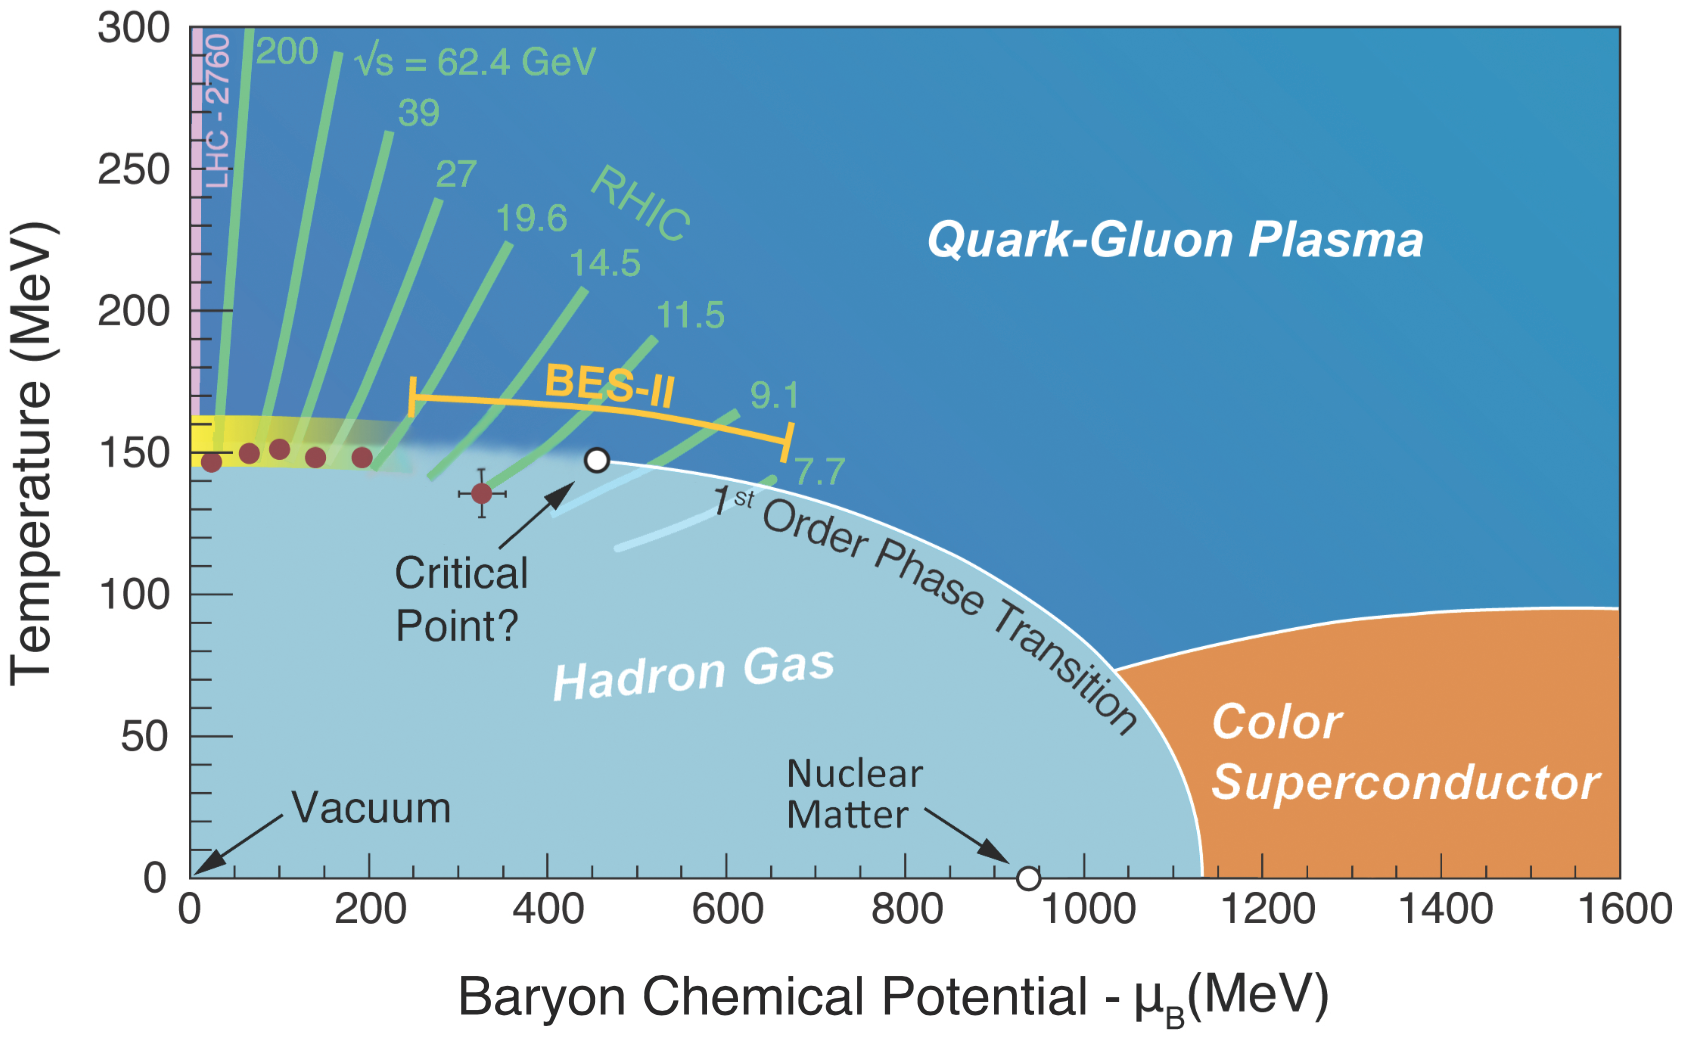
\includegraphics[width=.8\textwidth]{phase-diagram.png}
    \caption{The (partly projected) phase-diagram of the nuclear matter from reference []. The horizontal variable is Baryon chemical potentail $\mu_B$ and the vertical variable is temperature $T$. The red and green trajectories indicates the reachable regions by the heavy-ion program at the LHC and RHIC.}
    \label{fig:phase-diagram}
\end{figure}

Moving towards a finite baryon chemical potential, the lattice approach runs into the fermion sign problem, though recent studies has been pushing the realm of lattice QCD into regions of small $\mu/T$  \cite{Gunther:2016vcp,Bazavov:2017dus}.
Effective models [] and Dyson-Schwinger equation studies [] have suggested the existence of a first order phase transition at large $\mu_B/T$.
If true, the first-order coexistence line must end at a point on the phase-diagram at lower $\mu_b$, beyond which the phase-transition is of the cross-over type.
Such a point, called the critical end point (CEP), has attracted great interests from both the theoretical and the experimental community.

At higher chemical potential and low temperature, people conjectured another phase of nuclear matter known as the ``color superconducting phase'', where the quarks forms Cooper pair in analogy to superconductor [].

\begin{figure}
    \centering
    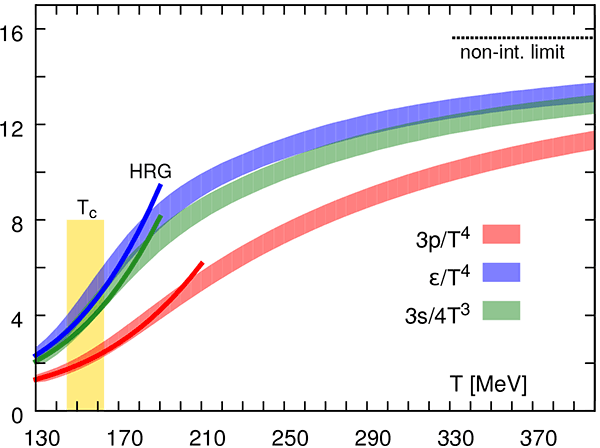
\includegraphics[width=.8\textwidth]{qcd-eos.png}
    \caption{The lattice equation of state for 2+1 flavor QCD taken from reference \cite{Bazavov:2014pvz}. The rescaled pressure, energy density and entropy density as function of temperature at zero chemical potential are shown as red, blue and green bands. The dashed lines indicates non-interaction (Stephan-Boltzmann) limit and the solid lines show the expected values from a hadron resonance gas. The yellow band is the region of pseudo-critical temperature.}
    \label{fig:qcd_eos}
\end{figure}

It is believed that the QCD high-temperature phase-transition occurred in the early universe around a microsecond after ``the Big Bang'', when its temperature drops down to the QCD scale.
Compact stars are ``celestial laboratories'' to test the QCD equation-of-state in the high density and low temperature region, providing an important physical input for simulating the recently discovered gravitational wave emission from neutron star mergers [].
In laboratories, we create hot and dense nuclear matter by colliding heavy nuclei at ultra-relativistic high energies.
While the created matter is transient and tiny compared to the cosmic nuclear matter, we can study not only thermodynamic properties but also essential dynamical properties of QCD in these experiments.

\section{Phenomenology of relativistic heavy-ion collision}
Relativistic heavy-ion collisions are currently the only tool to access the high energy density QCD medium in laboratory.
Since 2000, the Relativistic Heavy-ion Collider (RHIC) at the Brookheaven National Laboratory (BNL) has been colliding gold nuclei at 200 GeV []. 
The Large Hadron Collider (LHC) started its heavy ion programs later, colliding lead nuclei at 2.76 TeV and 5.02 TeV [].
Since then, evidences have been pointing to the existence a new state-of-matter: the strongly coupled quark-gluon plasma (sQGP).

In this section, I shall introduce useful concepts and terminology used in heavy-ion collision physics.
Then I will review a few important experimental observables and how they can help us understand the properties of the sQGP.

\subsection{Kinematics}
In ultra relativistic collisions, it is advantageous to use a new set of coordinates, related to the Cartesian coordinates by,
\begin{eqnarray}
x_\perp &=& x_\perp\\
\tau &=& \sqrt{t^2 - z^2}\\
\eta_s &=& \frac{1}{2}\ln\frac{t+z}{t-z}
\end{eqnarray}
where the $z$ direction aligns with the beam direction.
$\tau$ is called the ``proper time" and $\eta_s$ is called the space-time rapidity.
One advantage of using this set of coordinates is that $\tau$ and $\eta_s$ transforms much simpler than $t$ and $z$ under a Lorentz boost ($\beta_z$) in the beam direction,
\begin{eqnarray}
\tau' &=& \tau,\\
\eta_s' &=& \eta_s + \frac{1}{2}\ln\frac{1+\beta_z}{1-\beta_z}
\end{eqnarray}
Similarly, the four momentum $p^\mu$ is parametrized as 
\begin{eqnarray}
p_x &=& p_T\cos\phi\\
p_y &=& p_T\sin\phi\\
m_T &=& \sqrt{m^2 + p_T^2}\\
y &=& \frac{1}{2}\ln\frac{E+p_z}{E-p_z}.
\end{eqnarray}
$p_T$ is transverse momentum relative to the beam ($z$) direction, $\phi$ is the azimuth angle of particle emission. 
$m_T$ is referred as the transverse mass, and $y$ is the rapidity of a particle.
Besides, pseudorapidity is often used in experiments,
\begin{equation}
\eta = \frac{1}{2}\ln\frac{|p|+p_z}{|p|-p_z} = \frac{1}{2}\ln\frac{1+\cos\theta}{1-\cos\theta}
\end{equation}
It has the merits that it is directly related to the polar angle  $\theta$ of particle emission.
When the transverse mass is small compared to $p_z$, the pseudorapidity is also a good proxy of rapidity.

\subsection{Nuclear collision geometry}
Nuclei are extended objects.
The radius of heavy nuclei approximately scales like $A^{1/3}$ fm, where  $A$ is the atomic number; therefore, the collision geometry plays a far more important role than it is in the proton-proton collision.
In the center-of-mass frame,  nuclei ``shrink'' in the $z$ direction by the factor $\gamma = (1-v^2)^{-1/2} = E/M$ due to Lorentz contraction.
$\gamma$ is about $100$ for gold nuclei at top RHIC energy and is larger than $2500$ for lead nuclei at the LHC.
As a result, the approaching nuclei takes a very short time to penetrate each other $t_L = 2R/\gamma$, while dynamics in the transverse direction can only propagate within a causal circle of $r < t_L$ that is much smaller than the nuclear radius.

\paragraph{Impact-parameter and centrality} Defining the impact parameter $\vec{b}$ as the transverse separation between the centers-of-mass of the two approaching nuclei, the initial deposition of the energy largely depends on $\vec{b}$.
The collision geometry is a useful handle to study QGP dynamics; however,
it is impossible to control $b$ directly in high energy experiments.
What is used as an approximate geometry indicator is the so-called centrality.
Centrality is defined in different ways (detector response / multiplicity / transverse energy) and with different kinematic cuts, but the idea is that the nuclear collision geometry strongly correlates with the particle production activity.
It is reasonable to anticipate that the average number of charged particles produced or the total transverse energy deposited within a certain detector's acceptance is higher if the collision is more central (small impact parameter), and is lower for peripheral collision (large impact parameter).
Of course the relation between centrality and impact-parameter is not exact, as dynamical fluctuations smear out the one-to-one correspondence.
Correctly accounting for these fluctuations is particularly important for small collision systems, such as proton-lead and deutron-gold collisions.

\paragraph{Centrality selection} Experimentally, a minimum-biased (a minimum set of event triggers) sample of recorded events are sorted according to the centrality definition, e.g., multiplicity. 
Then the events are binned by percentile.
For example, the top 0--5\% highest multiplicity events are associated with centrality class 0--5\%. 
The collision geometry of a certain centrality class can then be studied through a model.
Usually, the model is one of many variants of the Glauber model \cite{Miller:2007ri}, which we shall explained it in detail in section \ref{chapter:simulation}).
It computes the number of binary nucleon-nucleon ($N_{\textrm{bin}}$) collisions and number of participant nucleons ($N_{\textrm{part}}$, nucleons that suffers at least one binary collisions) at a given impact parameter.
Experimentally, $N_{\textrm{part}}$ is often used as the centrality estimator of the model as it is roughly proportional to the bulk particle production; while the cross-section of hard processes that involves large momentum transfer $Q \gg \Lambda$ scales like the $N_{\textrm{bin}}$.
While this correspondence can be model dependent, the uncertainty can be quantified and model predictions can be validated by studying the production of colorless probes such as photon and weak-boson \cite{Afanasiev:2012dg,Chatrchyan:2011ua,Aad:2012ew,Aad:2015lcb,Adam:2015lda}.
In particular, recent measurement of $Z$ boson production in Pb-Pb collisions at $\sqrt{s}=5.02$ TeV has reached a very high precision to contrain collision geometry models in the future \cite{ATLAS:2017zkv}.

\subsection{Particle production at low-$p_T$ and collective flow} 
Immediately after the nuclei pass through each other at $t\sim 2R/\gamma$, a huge amount of energy is deposited into the overlap area and entropy is produced, creating a fireball in the middle while the nuclear remnants recede.
This highly excited fireball of fields undergoes complex dynamics and cools down rapidly due to its longitudinal and transverse expansion.
Eventually, the system hardronizes, and the hadrons can have further interactions and may decay into other hadrons, photons and lepton that are measured by the detectors.

It is observed that the particles produced in relativistic nuclear collisions are distributed across a wide (pseudo)rapidity range, and have steep falling transverse momentum spectra [].
The majority of the particles are soft hadrons with relatively small transverse momenta $p_T \lesssim 3$ GeV and their creation is a consequence of final state interactions [].
One of the most striking discoveries from the RHIC and the LHC heavy-ion programs is that these soft particles display a strong collectivity and the patterns can be described by viscous hydrodynamic-based models to a very high precision \cite{Dusling:2007gi,Song:2008si,Schenke:2010nt,Petersen:2008dd,Niemi:2015qia,Bernhard:2016tnd,Bernhard:2018hnz}.
This success of the hydrodynamic model reveals the strongly coupled nature of the matter produced with a temperature of several times $T_c$ and it has been given the name strongly coupled quark-gluon plasma.
This is in contrast to a weakly coupled gas of quarks and gluons that would not exhibit any collectivity.

\begin{figure}
\centering
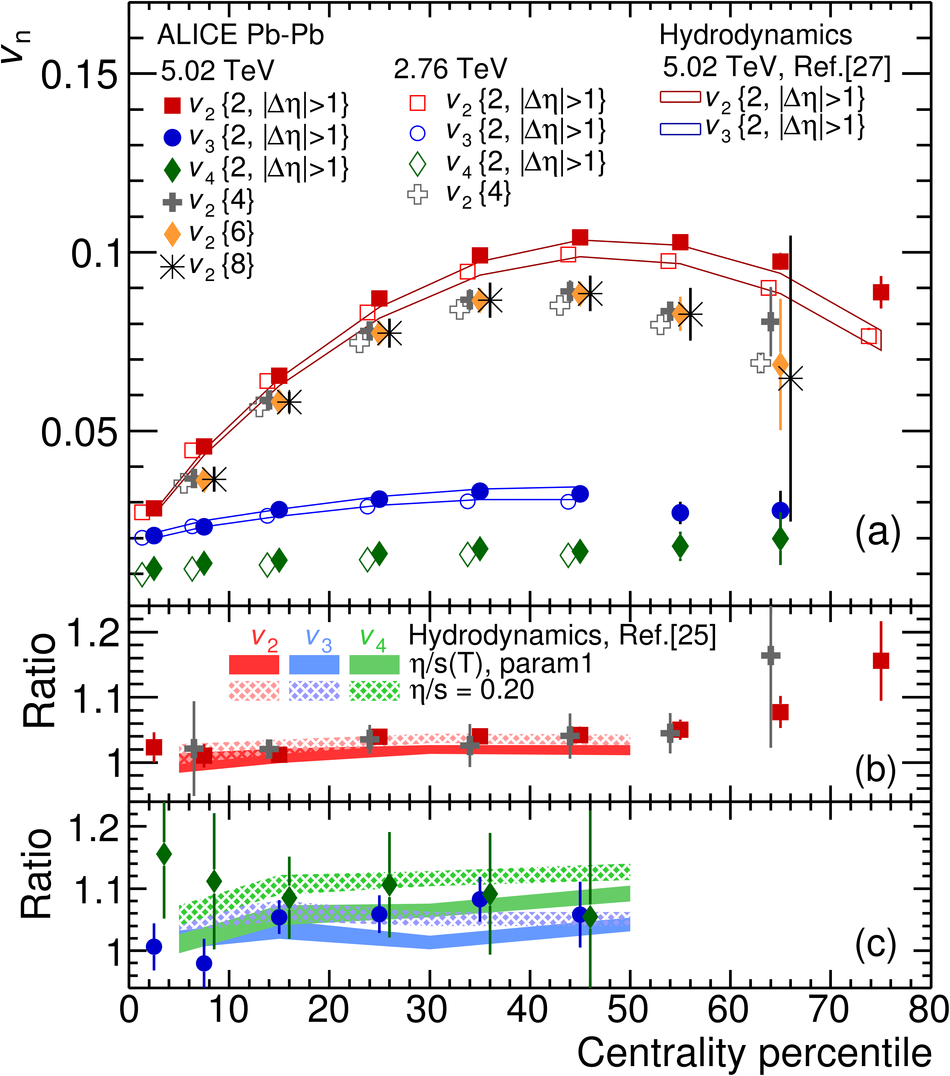
\includegraphics[width=.6\textwidth]{ALICE-chg-vn.png}
\caption{The momentum anisotropy coefficient $v_2$ estimated from multi-particle correlation for charged particle from the ALICE collaboration [].
The hydrodynamic-based calculations [] (lines) very well explains the centrality dependence of the second (red), third (blue) and fourth (green) order coefficients at different beam energies.}
\label{fig:intro:vn}
\end{figure}

One manifestation of collectivity is the momentum space anisotropy or collective flow of the bulk medium.
We decompose the charged particle spectra into a Fourier series of the azimuth angle,
\begin{eqnarray}
E\frac{dN}{p_T dp_T d\phi dy} = \frac{1}{2\pi}\frac{dN}{p_T dp_T dy}\left(1 + 2\sum_{n=1}^{\infty}v_n(p_T)\cos\left[n(\phi-\Psi_n)\right]\right).
\end{eqnarray}
The first term is an averaged yield, and subsequent terms in the sum encode the angular dependence. 
The $n=1$ term is a shift of the center-of-mass momentum
From $n=2$, $v_n$s are momentum anisotropy coefficients of $\cos({n\phi})$ modulations.
If the particle production is simply an independent sum of elementary nucleon binary collisions, then the anisotropy would be zero after the average. 
However, experiments observe a surprisingly larger elliptic flow ($v_2$), triangular flow ($v_3$) and higher order $v_n$ at both RHIC and LHC in nuclear collisions.
Figure \ref{fig:intro:vn} shows the variation of the $v_n$ as function of centrality from ALICE measurements [].
The $v_2$ coefficient first increases from central to mid-central collisions and slightly decreases at peripheral collisions, while $v_3$, $v_4$ signals are smaller and varies slower with centrality.

In the hydrodynamic picture, a non-central collision deposits initial energy density in an almond shape and the initial fireball has a finite spatial eccentricity $\epsilon_2$.
The energy density is higher in the middle and lower at the boundary, so a hydrodynamic pressure builds up and drives the transverse expansion of the fireball.
Because the pressure gradient is larger in the short axis-direction and the long-axis direction, the matter flows in an isotropic way, creating the observed momentum space second-order anisotropy $v_2$.
The existence of higher order of flow harmonics and non-zero $v_2$ in the most central collisions is because nuclear configuration fluctuations, such as randomized nucleon positions, create all orders of eccentricity $\epsilon_n$.
In short, a hydrodynamic expansion transfer initial geometry eccentricities $\epsilon_n$ into final state momentum anisotropy $v_n$ of the particle.

\paragraph{Extracting the QGP transport coefficients}
A relativistic ideal hydrodynamic model assumes an infinitely strong interaction that the medium always stays in local thermal equilibrium.
A more sophisticated treatment is relativistic viscous hydrodynamics which accounts for deviations from the local thermal equilibrium due to large gradients in the expansion.
The response of the hydrodynamic evolution to the gradients are characterized by the shear viscosity $\eta$ and bulk viscosity $\zeta$.
The QGP shear viscosity and bulk viscosity are of fundamental importance. 
The shear viscosity to entropy ratio $\eta/s$ is an indicator of the stong / weak coupling nature of the QGP. 
And the bulk viscosity to entropy ratio $\zeta/s$ is directly related to  the scale-invariance breaking of QCD.

Dynamical quantities such as viscosity are extremely hard to compute from first principle, so currently, the determination of these numbers and their temperature dependence requires phenomenological extraction from experiments \cite{Muronga:2004sf, Chaudhuri:2006jd, Romatschke:2007mq, Dusling:2007gi, Song:2007ux, Luzum:2008cw}.
The flow harmonics $v_n$ are particular sensitive to the viscous effects, as a finite viscosity dampens the development of anisotropic flows, reducing the transition efficiency from $\epsilon_n$ to $v_n$.
Global comparisons of the state-of-the-art medium modeling to a collection of soft observables have corroborated the need of a small $\eta/s$ that is likely to be slowly increasing with temperature and a non-vanishing $\zeta/s$.

\subsection{Probing sQGP using hard probes}
Very occasionally, an initial collision involving large momentum transfer creates high-$p_T$ particles in the system ($p_T\gtrsim 10$ GeV) that referred to as ``hard" particles.
By uncertainty principal, they can only be produced at the beginning of the nuclear collision on a time scale $\delta t \sim 1/p_T$, then they pass through and interact with the surrounding bulk medium.
Hard particles can be used as self-generated probes of the system.
Due to asymptotic freedom, the initial production of hard processes can be computed in the perturbative framework, granting a good theoretical control of its initial state.
The final state interaction with the medium then modifies the initial production and leaves finger prints of the medium on the hard probes.

\paragraph{Jet and jet quenching}
Initial hard partons (gluons, quarks) undergoes complex QCD dynamics, radiating more partons which then hadronize into a collimated bunch of hadrons and decay products.
This final collection of particles is observed in the detector as jets.
In proton-proton collisions, perturbative calculations and Monte-Carlo simulations are able to explain the production cross-section of the jet and leading hadrons (the hardest hadron in the jet) reasonably well.
In nuclear collisions, the initial parton and its radiative daugther partons interact with the medium, causing energy loss and triggering medium-induced radiation.
As a result, one expects the jet / leading parton yield at high-$p_T$ to be reduced compared to the reference in proton-proton collisions.
To focus on the difference caused by medium effects, the reference has to cancel out a na\"ive difference that simply rises because there are more effective nucleon-nucleon collisions in a nuclear collision.
One defines the so-called ``nuclear modification factor'',
\begin{eqnarray}
R_{AA}(y, p_T) = \frac{\frac{dN_{AA}}{dy dp_T}}{\langle N_{\textrm{coll}}\rangle \frac{dN_{pp}}{dy dp_T}} = \frac{\frac{dN_{AA}}{dy dp_T}}{\langle T_{AA} \rangle \frac{d\sigma_{pp}}{dy dp_T}}.
\end{eqnarray}
It is the average $N_{\textrm{bin}}$ ``normalized'' ratio between the yield in AA collisions and pp collisions.
The number of binary collisions is sometimes replaced by the average nuclear overlapping function $\langle N_{\textrm{coll}}\rangle = \langle T_{AA} \rangle /\sigma_{pp}^{\textrm{inel}}$, and the yield is replaced by the inclusive cross-section for the proton-proton collision $\frac{dN_{pp}}{dy dp_T}\rightarrow \frac{d\sigma_{pp}}{dy dp_T}$.
These two expressions are equivalent.
The ratio is expected to be unity if there is no medium effect, though we do remind the readers that $N_{\textrm{coll}}$ is not a directly observed quantity and has to be estimated in a model-dependent way.

At both RHIC and LHC, colored probes as measured by the $R_{AA}$ of leading hadrons and jets are found to be significantly below unity in nuclear collisions, while the $R_{AA}$ of color neutral probe such as $Z$-boson is consistent with unity \cite{Adare:2008qa,Chatrchyan:2011ua,Afanasiev:2012dg,Aad:2012ew,Aad:2015lcb,Adam:2015lda,ATLAS:2017zkv}.
These discoveries indicate the creation of a color deconfined medium that strongly modifies the hard parton propagation.
The interaction strength between the hard parton and the medium is theoretically quantified as the jet transport coefficient $\hat{q}$, which is defined as the momentum broadening per unit path-length in the transverse direction of the propagation,
\begin{eqnarray}
\hat{q} = \frac{d\langle p_\perp^2 \rangle}{dL}
\end{eqnarray}
The jet transport coefficient is another quantity of fundamental interest  in heavy-ion collisions, and there has been a great effort in both first principle computation and phenomenological extraction \cite{Wang:1994fx,Zakharov:1996fv,Baier:1996sk,Zakharov:1997uu,Arnold:2002zm,Gyulassy:2003mc,Kovner:2003zj,Jeon:2003gi,CasalderreySolana:2007pr,Djordjevic:2008iz,Bass:2008rv,Schenke:2009gb,Majumder:2009zu,Majumder:2010qh,Armesto:2011ht,Zapp:2011ya,Ovanesyan:2011xy,Kang:2014xsa,Cao:2016gvr,Kauder:2018cdt,Cao:2017zih}.
The hard parton / jet probes the medium at different scales at different stages of its evolution, and more sophisticated observables and theoretical tools are being constructed to answer more microscopic questions such as the actual degrees of freedom of the strongly coupled QGP.
Future experimental upgrades might provide the precision to look into this problems \cite{ATLAS-Collaboration:2012iwa,Abelevetal:2014dna,STAR:upgrade-hf,Adare:2015kwa,CMS:2017dec}.

\paragraph{Heavy-flavor probes}
Heavy flavor is also the major focus of this work.
Heavy quarks have masses well above the QCD non-perturbative scale.
The charm quark ($M=1.3$ GeV) and bottom quark (M=$4.2$ GeV) are the most relevant heavy quarks for the present study.
The reason that the top quark ($M = 173$ GeV) is out of our discussion is due to its extremely short life time ($\sim 5\times 10^{-25} \approx 0.15$  fm/$c$ in its rest frame) so it barely interacts with the QGP before it decays into, predominantly, bottom quarks.
Though there has also been a proposal that takes the advantage of this short life-time to probe the temporal structure of the QGP evolution \cite{Apolinario:2017sob}, we only focus on the charm and bottom flavor in this work.

\begin{figure}
\centering
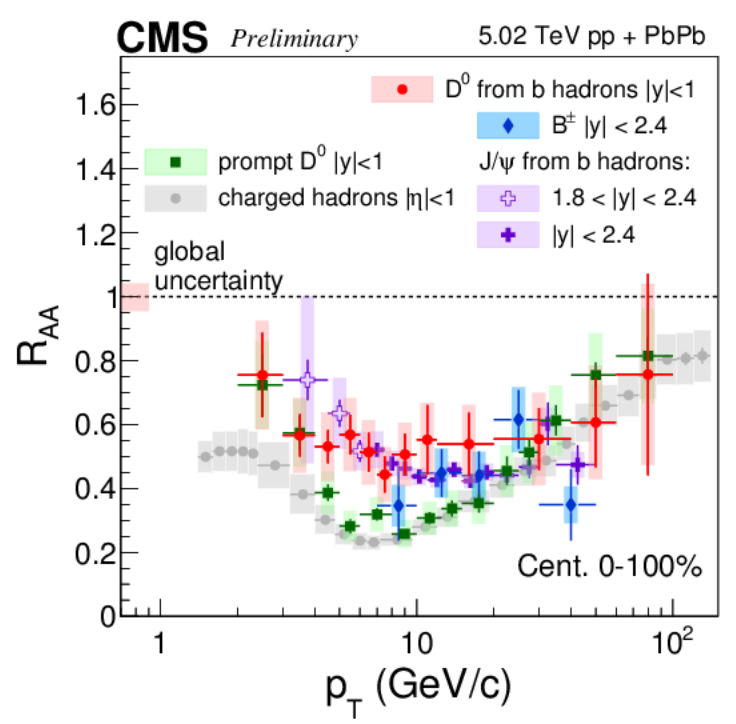
\includegraphics[width=.7\textwidth]{CMS-HF.png}
\caption{The nuclear modification factor $R_{AA}(p_T)$ of charged hadron (gray), D meson (red), B meson (blue), and $b$-decayed D meson (red), $b$-decayed J$/\Psi$ (purple) measured by the CMS collaboration [].}
\label{fig:intro:Raa}
\end{figure}

A large mass guarantees a negligible thermal production contribution, at least for the present top LHC beam energies (there are estimates that thermal contribution can play a role for the future FCC collider \cite{Zhou:2016wbo}).
Therefore, heavy flavors, regardless of $p_T$, are almost always created in initial hard processes.
Moreover, the tiny population of heavy flavors in the collision also suppresses the chances that they annihilate / recombine with their anti-particles.
Certainty heavy mesons have a long life time such that their decay vertices are outside of the fireball and can be resolved by experiments.
Therefore, the number of heavy-flavor particles is almost conserved from the beginning to the end of the entire medium evolution including both the QGP phase and the hadronic phase.

\begin{figure}
\centering
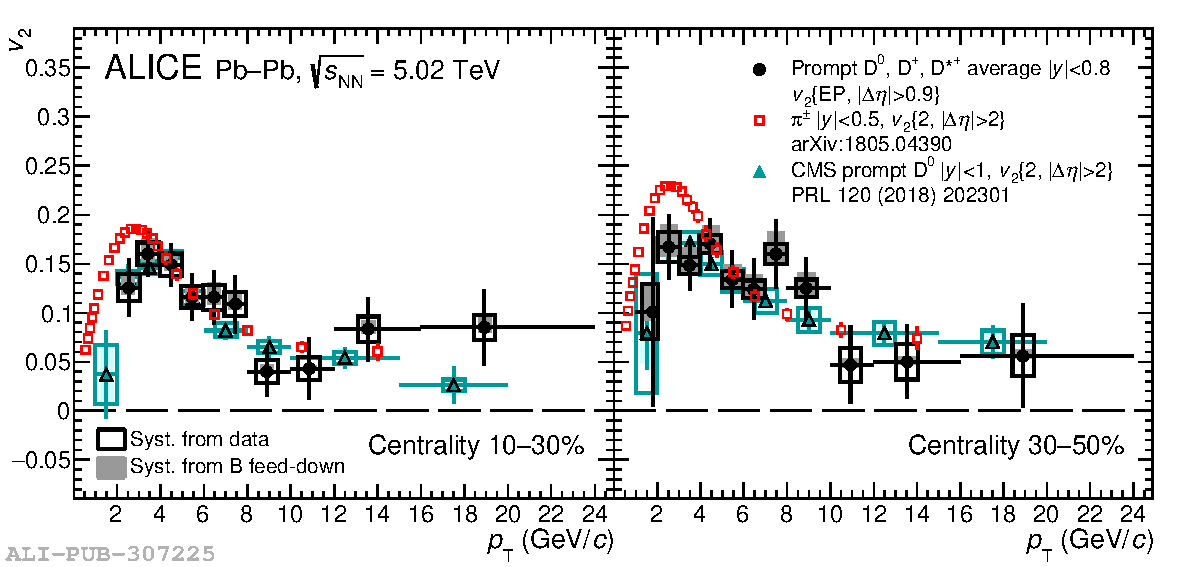
\includegraphics[width=\textwidth]{ALICE-CMS-D-vn.pdf}
\caption{The charged pion (red) and D meson momentum anisotropy measured by the ALICE Collaboration (black) and the CMS Collaboration (green). Left and right panels show the results for 10-30\% centrality and 30-50\% centrality respectively.}
\label{fig:intro:D-vn}
\end{figure}

Heavy flavors are of physical interests in many ways.
The mass effects are negligible at high $p_T$ where heavy flavors merge into the topic of the jet energy loss physics.
At intermediate $p_T$, the mass effect is expected to suppress the medium-induced radiation, which dominates the energy loss of light quark.
And there may be a competition between the collisional energy loss and radiation processes.
Experimentally, these differences lead to a hierarchy in the amount of nuclear suppression.
For example, figure \ref{fig:intro:Raa} from the CMS collaboration shows a collection of $R_{AA}$ measurements, for charged (mostly light) hadron, prompt D meson, prompt B meson and D and J/$\Psi$ from $b$-decays.
All the $R_{AA}$ tends to collapse onto the same trend at very high-$p_T$, while for $p_T$ range aounrd 5 to 20 GeV, despite the large uncertainty, there is a suggestive hierarchy of $R_{AA}(\textrm{light}) < R_{AA}(\textrm{charm}) < R_{AA}(\textrm{bottom})$.
It would be interesting to study whether a theoretical framework can explain this difference quantitatively and distinguish different energy loss mechanisms.

Low-$p_T$ heavy quark physics is even more interesting.
In this region, collisional process dominates over radiative process, and the description of the heavy quark dynamics under the influence of medium ``kicks'' reduces to a succinct diffusion equation \cite{Moore:2004tg}.
A spatial diffusion constant $D_s$ controls the close-to-equilibrium dynamics, and canbe related to the momentum diffusion by $D_s = 4T^2/\hat{q}(p\rightarrow 0)$.
The large inertia $M\gg T$ delays its relaxation time $\tau_{\textrm{th}} \propto M/T D_s$ and one expects to find a different degree of thermalization for light, charmed, and bottom hadrons \cite{PhysRevD.37.2484,Moore:2004tg,Riek:2010fk,Cao:2013ita}.
For instance, looking at the low $p_T$ momentum anisotropy of charmed meson shown in figure \ref{fig:intro:D-vn} \cite{Acharya:2017qps,Sirunyan:2017plt}.
The large $v_2$ of the charged pions below $3$ GeV is due to the collective expansion.
The charmed mesons also catch up a significant amount of flow \footnote{As a remark, the finite $v_2$ of D meson at high $p_T$ is not directly related to the flow phenomena, but as a result of anisotropic energy loss in a spatial eccentric medium}, though still less than the pion.
To explains this amount of D meson $v_2$, phenomenological studies suggests a $D_s$ close to the lattice QCD calculations \cite{He:2012df,Cao:2013ita,Xu:2017obm,Banerjee:2011ra,Ding:2012sp,Francis:2015daa}, while leading order weakly coupled result \cite{Moore:2004tg} is inadequate . 
This finding suggests the importance of non-perturbative phenomenon in understanding the coupling between low momentum heavy quark and the medium.

Finally, the unique flavors of heavy quarks help to tag certain processes of interest. 
For example, the study of recombination hadronization mechanism, strangeness enhancement, and implementation of a selection bias on the quark / gluon-initiated jet ratio.

\subsection{Transport modeling of hard probes}
The understanding of jets and heavy-flavor in heavy-ion collisions needs a comprehensive non-equilibrium modeling effort.
This includes initial production / DGLAP evolution, partonic propagation in the QGP, and eventually hadronic interaction.
Transport equations are convenient tools to couple the microscopic hard probes propagation to the macroscopic medium evolution, though one has to be very careful with the multiple scales of the problem.
For example DGLAP evolution brings the parton scale from $p_T$ down to O(GeV).
The probe-medium interactions happens at typical scales around temperature $T$ and the screening mass $m_D \sim gT$, while the medium-induced radiation occurs at a momentum broadening scale of order $\hat{q} t$.
Eventually, hadronization happens at scale $\Lambda$.
Meanwhile, the medium evolution has a another set of (time) scales, the hydrodynamization time $\sim 1$ fm/$c$, the finite-size and life-time of the QGP fireball $\sim O(10)$  fm/$c$, and the expansion time scale $\tau_{\textrm{ex}}$.
Usually a separation of scales allows great simplification to theory calculations.
For example, the Boltzmann transport equation requires a separation between the mean-free-path and the coherence time of the scattering.
However, in realistic event simulations, treating regions of overlapping scales seems inevitable.
We would like to develop in this thesis a new transport model to account for a few of these overlapping scale issues.

\paragraph{Heavy quark transport models}
In early days, the heavy quark measurements at RHIC energy did not extend to very high-$p_T$ and the radiative energy loss is not as important as elastic ones.
Therefore, earily studies relied on non-equilibrium dynamics using a pure diffusion model \cite{Moore:2004tg,vanHees:2007me}. 
To include physics at high-$p_T$ physics, a radiation improved diffusion model was then developed \cite{Cao:2013ita} and has been applied to the first Bayesian extraction of the heavy quark transport coefficients \cite{Xu:2017obm}.
Apart from the diffusion-based models, Boltzmann and linearized Boltzmann models, including both elastic and inelastic interactions, has also been developed \cite{Scardina:2017ipo,Cao:2017hhk,Ke:2018tsh}.
Regarding the physical inputs, the Boltzmann-based model takes a weakly-coupled picture; the diffusion based model is more flexible, since the transport coefficient can be computed in both weakly coupled or strongly coupled approaches.
Using different models, the extracted transport parameters $D_s$, $\hat{q}$ have notable differences \cite{Rapp:2018qla,PhysRevC.99.014902,Cao:2018ews}.
The major sources that leads to these differences are:
\begin{itemize}
\item Inclusion of radiative energy loss.
\item Assumptions on the medium: close-to-equilibrium hydrodynamic medium, or non-equilibirum medium from a full partonic Boltzmann equation.
\item Weakly coupled approach versus strongly coupled approach.
\item More subtle differences such as Langevin versus Boltzmann dynamics, and the detailed treatment of the radiative processes.
\end{itemize}
To make progress,improved theoretical calculations and more accurate modeling is important; on the other hand, more subtle differences can be treated as intrinsic modeling uncertainty so that the extracted transport parameters are not over-interpreted (a finite theoretical uncertainty bands on $D_s$ and $\hat{q}$). 

\subsection{Understanding QGP as a parameter inference problem}
All the interesting dynamics of heavy-ion collisions last for $O(10) $ fm/$c$, while we can only observe the collision remnants by detectors meters away.
Therefore, the determination of any intrinsic properties of the QGP is essentially  a parameter inference problem:
given measurements, models, and parameters of QGP such as $\eta/s, \hat{q}$, what is the favored range of parameters to explain the data.
Finally, by comparing the theoretical expectations and the phenomenological constraints of these parameters, one can evaluate the theoretical assumptions, which provide new information on the QGP.

This inversion from observables to parameters is not as simple as it appears, because of the following difficulties,
\begin{itemize}
\item The dynamical models are complex and computationally expensive.
\item Models take multiple parameters or unknown functions that have infinitely many degrees of freedom.
\item Global comparison to many experimental observables.
\item The quantification of uncertainty: including experimental uncertainty, model uncertainty and theoretical uncertainty.
\end{itemize}
Most of these issues can be solved by a Bayes analysis for model parameter calibration, and its key ingredients will be explained in chapter \ref{chapter:bayes}.
A remaining issue is the theoretical uncertainty, which is hard to quantify.
Our solution to the theoretical uncertainty is two-fold.
First, if there exist more than one theoretical assumptions without compelling reasons to disfavor either of them, then this difference should be propagated into the extracted model parameters.
Including these uncertainty will certainly decrease the constraining power on the transport parameters, but it prevents biasing the estimated number from imposing a too strong assumption.
Second, existing theoretical calculations are often worked out in certain idealized limits, while a dynamical modeling approach is much more complicated and may not closely follow the underlying theory.
This will certainly obscure the interpretation of the extracted parameters.
Therefore, as an important practice for dynamical modeling, the model should be able to calibrate to theoretical calculations at least in those idealized limits, and then be generalized to the more complex scenario.
We devoted chapter \ref{chapter:transport} to improve the accuracy of hard parton transport model.

\section{Outline of this Thesis}
In this thesis, I focuses on the extraction of the heavy quark transport coefficients from experiments using a newly developed transport model for hard parton in a quark-gluon plasma.
In chapter \ref{chapter:simulation}, I introduce a hydrodynamic-based medium for the medium evolution. 
As an application of this simulation framework, I review my project on reverse engineering a three-dimensional initial entropy deposition of the heavy-ion collision from experimental data. 
In chapter \ref{chapter:transport}, we develop the transport model for hard partons (including heavy flavors) propagation inside a quark-gluon plasma.
This model interpolates a small-angle diffusion picture and a large-angel scattering picture of the probe-medium interaction.
I show the limitation of the semi-classical transport approach in implementing parton branching processes (radiation) at high energy, and demonstrate how to modified the semi-classical approach to treat it properly.
Chapter \ref{chapter:coupling} builds a comprehensive simulation workflow that couples the initial production and in-meidum transport of heavy flavors to the bulk medium evolution.
Benchmark calculations with simple guesses of parameters are compared to the experimental measurements.
Chapter \ref{chapter:bayes} is a brief description of the Bayes methodology of model parameter calibration.
Applying the Bayes method, in chapter \ref{chapter:results}, a systematic model-to-data comparison is performed, extracting the heavy flavor transport properties.
Finally, chapter \ref{chapter:conclusion} summarizes the work and discuss possible future improvements.



\chapter{Bulk medium evolution and initial condition}
In this chapter, I shall introduce a hydrodynamic based model for describing the bulk medium evolution in the heavy-ion collision.
After the basic description of the modeling, I will show an application of this simulation framework in reverse engineering the three-dimensional initial entropy deposition, which is one of my published research projects.

\section{A Hydrodynamics-based multi-stage modeling}
\subsection{The hydrodynamic equations}
There has been vast experimental evidences that supports the use of an relativistic viscous hydrodynamics in describing the dynamical evolution of the medium created in the heavy-ion collision.
At mid-rapidity, the hydrodynamic-based model can achieve a high precision of agreement with a global comparison to experimental data. 
This data also support the use of a small but nonzero specific shearviscosity {Muronga:2004sf, Chaudhuri:2006jd, Romatschke:2007mq, Dusling:2007gi, Song:2007ux, Luzum:2008cw}, and more recent studies and global Bayesian analysis also suggest the use of a finite bulk viscosity.

\paragraph{Ideal hydrodynamics} Hydrodynamics is a macroscopic description that propagates the energy momentum tensor of the system without an microscopic knowledge of the degrees of freedom.
The first four equations comes from the the energy-momentum conservation,
\begin{eqnarray}
\partial_\mu T^{\mu\nu} = 0
\end{eqnarray}
where $T^{\mu\nu}$ is the energy momentum tensor and $\partial_\mu = \partial/\partial x^\mu$. 
Here we have choose the metric as $g^{\mu\nu} = \diag\{1, -1, -1, -1\}$.
If one assumes ideal hydrodynamics that the system always relax to local thermal equilibrium fast enough compared to other time scale, then $T^{\mu\nu}$ can be expressed as
\begin{eqnarray}
\partial_\mu T^{\mu\nu} = e u^\mu \nu - P (g^{\mu\nu}-u^{\mu\nu})
\end{eqnarray}
where $u^\mu$ is the flow velocity such that in the co-moving frame  $T^{\mu\nu}$ has the diagonal form $T^{\mu\nu} = \diag\{e, -P, -P, -P\}$.
Therefore $e$ and $P$ are the energy density and pressure of the thermalized matter in the rest frame.
There are five unknowns $e, P, u_x, u_y, u_z$ ($u_t$ is determined by $u^2 = 1$), but conservation laws only provide four equations.
A fifth equation is the equation of state (EoS) $P = P(e)$ that encodes thermodynamic properties of the medium (in this case, the nuclear medium at finite temperature) which closes the set of ideal-hydrodynamic equation.
\paragraph{Inputs from first principal calculation} The lattice QCD simulation has determined the QCD equation of state to high precision with physical masses of the light flavor.
It is not a prior known that the lattice QCD EoS computed for an infinite matter in infinite time is the best choice for describing a transient, finite size system, however, using the lattice input does result in reasonable agreement with the data.
Moreover, there has been a study that try to constrain the from of EoS from experimental data and the ``calibrated'' EoS is very close the Lattice prediction.
Most of the currently hydrodynamic studies already uses the state-of-the-art lattice results.
\paragraph{Viscosity correction and QCD transport coefficient}
The medium created in heavy-ion collision undergoes fast longitudinal and transverse expansion, and the thermalization rate may not be fast enough to keep the system in fully thermal equilibrium,
\begin{eqnarray}
T^{\mu\nu} = u^\mu u^\nu e - (g^{\mu\nu}- u^\mu u^\nu) (P+\Pi) + \pi^{\mu\nu}
\end{eqnarray}
Here $T_0$ is the thermal part, and $\pi$ is the shear viscosity correction, and $\Pi$ is the bulk viscosity correction to the pressure.
Relativistic viscosity hydrodynamics that expands the transport description in terms of the Knudsen number is developed to taken into account viscous effects.
At first order, this is well-known Naiver-Stokes equations, where the $\pi$, $\Pi$ are given by the constitutive relations,
\begin{eqnarray}
\pi^{\mu\nu} &=& 2\eta\sigma^{\mu\nu}\\
\Pi &=& -\zeta\theta
\end{eqnarray}
Here the corrections to the energy momentum tensor are proportional to the first gradient of the macroscopic field $\sigma^{\mu\nu} = \partial^{\langle \mu} u^{\nu\rangle}, \theta = \partial\cdot u$.
The proportional constant are known as the (first order) transport coefficient of the QCD matter, which encodes the dynamical information of the system. 
Especially their dimensionless ratio to the entropy density $\eta/s$ and $\zeta/s$ are important indicator of the interaction strength and the scale-violation of the QCD matter and are of great physical importance.
There have been many effort to either computing these quantities from first principles and effective models or extracting these numbers in a model-to-data comparison.
Coming back to the hydrodynamic modeling, it is shown that one has to go to second order in the expansion to the render the correction compatible with special relativity and $\pi$, $\Pi$ becomes dynamical quantities which tends to relax to the Naiver-Stokes limit.
\begin{eqnarray}
\nonumber
\tau_\pi \dot{\pi}^{\langle\mu\nu\rangle}+\pi^{\mu\nu} &=& 2\eta\sigma^{\mu\nu}- \delta_{\pi\pi}\pi^{\mu\nu}\theta + \phi_7 \pi_{\alpha}^{\langle\mu}\pi^{\nu\rangle\alpha}-\tau_{\pi\pi}\pi_{\alpha}^{\langle\mu}\sigma^{\nu\rangle\alpha} + \lambda_{\pi\Pi}\Pi\sigma^{\mu\nu},
\\
\nonumber
\tau_{\Pi}\dot{\Pi} + \Pi &=& -\zeta\theta - \delta_{\Pi\Pi}\Pi\theta + \lambda_{\Pi\pi}\pi^{\mu\nu}\sigma_{\mu\nu}.
\end{eqnarray}
The $\delta, \phi, \lambda$ are known as second order transport coefficients.
This complicated set of equations together with the conservation law and the EoS forms the viscosity hydrodynamic equations.
Nowadays, well tested numerical packages have been developed solving these equations in the context of heavy-ion collisions.

\paragraph{Boost-invariance approximation and beyond}
In general, the hydrodynamic equations have to be solved as a 3+1 dimensional problem.
But a reduction to a 2+1 dimension is possible, if one assume the fast expansion along the beam-axis (longitudinal) direction has an approximated symmetry near mid-rapidity.
This approximate symmetry is first proposed by Bjorken in [] that the system at different rapidity looks similar upto a longitudinal boost, so that one may first obtain the solution to the 2+1 dimension problem at one space-time rapidity ($\eta_s = 0$) and then boost the solution to other $\eta_s$.
A direct consequences of this symmetry is that the observables should not depends on space-time rapidity.
The $\eta_s$-dependence cannot be directly detected, but can be related to the the rapidity / pseudo-rapidity for the reason below.
Suppose that the Lorentz contracted nuclei interact at $z=0$ and produce excitations that free-stream in the longitudinal direction, then for each of these excitation
\begin{equation}
  \frac{z}{t} = \frac{p_z}{E}.
\end{equation}
This approximation the equivalence of $\eta_s$ and $y$ at early stages of the collision:
\begin{equation}
  \eta_s = \frac{1}{2}\log\frac{t+z}{t-z} \sim y = \frac{1}{2}\log\frac{E+p_z}{E-p_z}.
\end{equation}
If one further assumes these initial excitations are mass-less partons, then the rapidity can be approximated by pseudorapidity as $E\approx |p|$.
The event-averaged rapidity-distribution of charged particles $dN_{\textrm{ch}}/dy$ in both proton-proton and symmetric nuclei-nuclei collisions at the LHC energy falls at large rapidity but has a slowly varying profile at mid-rapidity within $|y|<2$, which is a motivation to apply the boost-invariant at mid-rapidity as a first approximation.

However, since $dN_{\textrm{ch}}/dy$ are event-averaged quantities, its being flat within $|y|<2$ does not rule out that event-by-event particle production fluctuation can break the approximation, and these fluctuations, local in transverse plane, can be different at different transverse location.
Moreover, asymmetric nuclear collision such as $p+Pb, p+Au, d+Au, He+Au$, etc clearly breaks the boost-invariance even on an event averaged level. 
Therefore, the study of longitudinal fluctuation related observables or the search for hydrodynamic  behavior in small collision system clearly requires one to go beyond the boost-invariance approximation.

\subsection{Particularization and microscopic transport}
The longitudinal expansion and the transverse expansion driven by the pressure difference cools down the system temperature and density rapidly and eventually the relaxation rate is too low for the the hydrodynamic approach to apply.
When this happens, one can switch to the microscopic transport description of the system.
This switching is usually done near or below the pseudo-critical temperature $T_{sw} \lesssim T_c$ so that the energy momentum tensor can be particularized as an ensemble of hadrons .
This choice $T_{sw} \lesssim T_c$ avoids the problem of modeling quark / gluon dynamics and hadronization in the strong coupled regime near $T_c$, and whether a hydrodynamics with lattice EoS and a hadronic transport model with cross-sections as inputs are both valid in this regime is another question.
The hydrodynamic $T^{\mu\nu}$ is usually particlized at a constant energy density / temperature hypersurface using the Cooper-Frye formula,
\begin{eqnarray}
dN_i^a(p) = \frac{g^a f^a(p) dp^3}{(2\pi)^3}  \frac{p^{\mu}}{E} \Delta \sigma_{i,\mu} 
\end{eqnarray}
Where the particle yield of specie ``$a$'' with momentum $p$ from the $i^{\textrm{th}}$ surface element $\sigma_{i,\mu}$ equals its phase space density times the surface area (with units of a 3D volume) parallel to the  four velocity $p^\mu/E$.
This distribution function should include both a thermal part and a viscous correction, $f = f_0 + \delta f$.
There are more than one way to construct the viscous correction $\delta f$  from $e, P, n, \Pi$ and $\pi^{\mu\nu}$ based on different assumptions of the form of corrections.
In this work, we shall use a non-additive $\delta f$ correction that has been developed and implemented by [] and [], and please refer to the references for the original formulation and numerical implementations details.

The particlized hadronic system is then solved by the Ultra-relativistic Quantum Molecular Dynamics (UrQMD) model until the system is dilute enough and interactions ceases (kinetic freezeout). 
The UrQMD in the context of hadronic cascade (afterburner) includes processes like resonance decays, elastic and inelastic scatterings, and string formations and fragmentations.

\subsection{Pre-equilibrium stage}
At very early times of the collision, the system is off equilibrium. 
However, viscous hydrodynamic assumes a closeness to the local thermal equilibrium  (there are also recent efforts in studying the effectiveness of hydrodynamics outside of its traditional range of application []).
A successful prediction using an early onset of hydrodynamic evolution at $\tau_0\lesssim 1$fm/$c$ suggests a fast hydrodynamization, whose exact mechanism is still a debatable question. 
There are different modelings of this pre-equilibrium stage, including solving the classical Yang-Mills equation [], partonic transport models [], a collision-less Boltzmann equation [], and the linear response method of the effective kinetic approach [].

Such a pre-equilibrium stage was not included in my study of the 3D initial condition, where the simulation starts at $\tau_0 = 0.6$ fm/$c$ assuming local thermal equilibrium.
For my later study of the heavy flavor dynamics, a 2+1D collision-less Boltzmann equation implemented by [] was later used in obtaining the medium evolution history.
In such a model, the initial energy density ($\tau = 0^+$) at mid-rapidity  is thought to be carried by mass-less partons that propagates at the speed of light in the transverse direction. 
The initial distribution function is assumed to have a factorized form $f(x_\perp, p_\perp, \tau=0) = n(x, \tau=0) \times dN/dp_\perp^2$.
The momentum distribution $dN/dp_\perp^2$ do not evolve as the collisions are neglected, while the spatial density evolves as
\begin{eqnarray}
n(\vec{x}, \tau) = \int n(\vec{x}', \tau=0) \delta^{(2)}(\vec{x} - \vec{x}'- \tau) d\vec{x}'^2
\end{eqnarray}
Then, the model assumes a sudden hydrodynamization at time $\tau_{\textrm{hydro}}$, where the free-streamed,
\begin{eqnarray}
T^{\mu\nu}(x_\perp, \tau_{\textrm{hydro}}) = \int f(x_\perp, p_\perp, \tau=0) \frac{p^\mu p^\nu}{E} dp^3
\end{eqnarray}
is used for initializing the hydrodynamic equations by the Landau matching procedure [].

\subsection{Initial condition}
Unlike the dynamical models that are governed by a few equations / laws with a few parameters, the initial condition model parameterizes many more unknowns.
For different initial condition models, these unknowns can be initial color density of the nuclear wave function, the effective size of a nucleon, the form factor of nucleon-nucleon inelastic cross-section, and the amount of fluctuations in particle production / energy deposition, etc.
There are two classes of initial condition models:
\begin{itemize}
\item Models that takes into the particle production dynamics. Such as minijet production, strings productions and flux-tubes, hadronic transport,and color-glass condensate (CGC) effective field theory based models {Wang:1991hta, Zhang:1999bd, Werner:2010aa, Petersen:2008dd, Schenke:2016ksl, Dumitru:2011wq, Hirano:2012kj}.
\item Parametric models that provides macroscopic initial conditions without a dynamical component. Such as Monte-Carlo Glauber models and its extensions [Bozek:2015bna], and the \trento model to be explained [Scott].
\end{itemize}
I shall focus on the development of a parametric model \trento to help the understanding of the initial three-dimensional entropy deposition.


\paragraph{The original (boost-invariant) \trento\ model}
The original \trento\ model is proposed as a flexible ansatz to investigate a family of entropy / energy deposition behaviors at mid-rapidity.

First, the impact parameter $\vec{b}_{AB}$ between the two colliding nuclei $A$ and $B$ is sampled at random.
Then, the 3D nucleons positions inside each nuclei are sampled according to the Woods-Saxon distribution (for heavy nuclei, for light nuclei such as Deuteron, Helium, Oxygen where the nucleon distribution is not well approximated by a Woods-Saxon form, the sampling are different),
\begin{eqnarray}
\frac{df_N}{r^2 dr d\phi d\cos\theta} = \frac{1}{\exp\{\frac{r-R(1+\beta_2 Y_{20}(\theta)+\beta_4 Y_{40}(\theta))}{a}\}+1}
\end{eqnarray}
including the quadrupole and hexadecapole deformation of certain nuclei.
The randomized nucleon position is critical to explain the odd order of flow harmonics observed in experiments [].

Then, the collision between the two nuclei is analyzed at the nucleon level. 
Every nucleon pair $\{i, j\}$ with $i$ from nuclei $A$ and $j$ from nuclei $B$ has a certainty probability to undergo an inelastic collision, given the impact parameter $\vec{b} = \vec{b}_{AB} + \vec{x}_{i, \perp} -  \vec{x}_{j, \perp}$,
\begin{eqnarray}
P(b; \sigma) = 1 - \exp\left[-\sigma T_{pp}(b)\right],
\label{dsigma_db}
\end{eqnarray}
where $T_{pp}(b)$ is the overlapping function between the density of the nucleon,
\begin{eqnarray}
T_{pp}(b) = \int d\vec{x}_\perp^2 T_p(\vec{x}_\perp-\vec{b}/2) T_p(\vec{x}_\perp+\vec{b}/2)
\end{eqnarray}
And each nucleon is assumed to have a Gaussian density profile, 
\begin{eqnarray}
T_p(\vec{x}_\perp^2) = \frac{1}{2\pi w^2} \exp\left(-\frac{\vec{x}^2}{2w^2}\right)
\end{eqnarray}
with the width of the nucleon $w$ a free parameter.
The $\sigma$ is an effective constituent cross-section that is determined by reproducing the experimental measured proton-proton inelastic cross-section at a given beam energy,
\begin{eqnarray}
\sigma_{pp}^\text{inel}(\sqrt{s}) = \int d\vec{b}^2 P(b; \sigma(\sqrt{s}))
\end{eqnarray}


\paragraph{Parametrize the longitudinal dependence in \trento}



In the present study we seek to parametrize and constrain the full three-dimensional structure of the produced QGP medium.
It is thus essential that any resulting model maintain good agreement with charged particle multiplicity distributions and flow harmonics at midrapidity.
We consequently adopt a factorized approach and express the initial entropy density $s$ at the hydrodynamic starting time $\tau_0$ as
\begin{equation}
  s(\x, \eta_s)\vert_{\tau=\tau_0} \propto f(\x) \times g(\x, \eta_s),
  \label{factorized}
\end{equation}
where $\x = (x, y)$ is a position in the transverse plane, $\eta_s$ is the spacetime rapidity, $f$ denotes the entropy density in the transverse plane at midrapidity, and $g$ is some rapidity-dependent function such that $g(\x, 0)=1$.

\subsection{Midrapidity calculation}
We simulate entropy deposition at midrapidity using the parametric model \trento\ {Moreland:2014oya}, which is constructed to interpolate a subspace of all initial condition models including (but not limited to) specific calculations in CGC effective field theory.
The initial condition model was recently embedded in an event-by-event hybrid model which couples viscous hydrodynamics to a microscopic kinetic description {Shen:2014vra} and its parameters constrained using Bayesian parameter estimation {Bernhard:2016tnd}.
Here we briefly summarize its key features.

The model samples independent nucleon positions from spherical (or deformed) Woods-Saxon density distributions, shifts the nucleons in each nucleus by a random impact parameter offset $b$, and projects each coordinate onto the transverse plane.
Participant nucleons are then sampled according to the pairwise inelastic collision probability

where $b$ is now the impact parameter between two nucleons, $\sigma_{gg}$ is an effective partonic cross section tuned to fit the measured inelastic proton-proton cross section at a given beam energy, and $T_{pp}$ is the proton-proton overlap function
\begin{equation}
  T_{pp}(b) = \int d^2\x\, T_p(\x)\,T_p(\x - \mathbf b).
\end{equation}
The proton thickness function $T_p$ is described by a simple Gaussian density profile
\begin{equation}
  T_p(\x) = \frac{1}{2 \pi w^2} \exp\bigg({-}\frac{\x^2}{2 w^2}\bigg),
  \label{nucleon_profile}
\end{equation}
with effective proton width $w$.
Once the participants in each nucleus are determined according to Eq.~\eqref{dsigma_db}, a participant nuclear thickness function $\T$ is constructed by summing the proton thickness function of each wounded nucleon, e.g., the participant thickness function of nucleus $A$ is given by
\begin{equation}
  \T_A(\x) = \sum\limits_{i=1}^{N_\text{part}} w_i\, T_p(\x - \x_i).
\end{equation}
Here $w_i$ is a random weight sampled from a gamma distribution with unit mean and variance $1/k$, where $k$ is a tunable shape parameter.
This additional source of fluctuation is added to reproduce the negative binomial distribution of the charged particle multiplicity in minimum bias proton-proton collisions {Bozek:2013uha}.

Initial entropy deposition at midrapidity is then described by an eikonal function $s(\x, 0) \propto f(\x)$ which maps participant nucleon density to local entropy deposition.
For this mapping, the \trento\ model adopts a flexible parametric form known as the generalized mean,
\begin{equation}
  \label{gen_mean}
        f(\x) \propto \left( \frac{\T_A^p + \T_B^p}{2} \right)^{1/p},
\end{equation}
where the continuous parameter $p$ smoothly interpolates among different types of entropy deposition schemes {Bernhard:2016tnd}.
For example, $p=1$ is exactly a wounded nucleon model, while $p\sim-0.67$ simulates entropy deposition in the original KLN model {Drescher:2006ca}, and $p \sim 0$ closely mimics the behavior of both IP-Glasma {Schenke:2012wb} and EKRT {Niemi:2015qia} saturation calculations.

\trento\ initial condition parameters have been constrained using Bayesian parameter estimation and calibrated to fit identified particle yields, mean transverse momenta, and flow cumulants in ${\sqrts=2.76}$~TeV Pb+Pb collisions {Bernhard:2016tnd}.
The analysis established 90\% credible intervals for the effective nucleon width {$w \approx 0.5 \pm 0.1$ fm} and entropy deposition parameter ${p \approx 0.0 \pm 0.2}$, while the nucleon fluctuation shape parameter $k$ was essentially unconstrained by data.
Corresponding model predictions simultaneously fit charged particle yields, mean transverse momenta, and flow cumulants at the 10\% level or better across all centralities and hence corroborate the effective initial condition mappings predicted by IP-Glasma and EKRT theory calculations.


\subsection{Extension to nonzero rapidity}

The factorized expression in Eq.~\eqref{factorized} extends entropy deposition at midrapidity $f(\x)$ to nonzero rapidity using a rapidity-dependent mapping $g(\x, \eta)$ which multiplies $f$ to incorporate nontrivial longitudinal structure.
Before constructing the form of this longitudinal dependence, we elucidate our use of spacetime rapidity $\eta_s$, rapidity $y$, and pseudorapidity $\eta$.

Therefore, we first parametrize the rapidity dependence of the system and then perform a change of variables from $y$ to $\eta$ using the relations
\begin{align}
  g(\x, \eta)\, d\eta &= g(\x, y)\, dy, \\[1ex]
  \frac{dy}{d\eta} &= \frac{J \cosh \eta}{\sqrt{1 + J^2 \sinh^2 \eta}},
  \label{jacobian}
\end{align}
where the species-dependent factor $J$ is replaced with an effective value $J \approx \langle p_T \rangle / \langle m_T \rangle$.
We then invoke $\eta_s \sim \eta$ for an initial condition of massless partons, so that the rapidity-dependent entropy profile is
\begin{equation}
  s(\x, \eta_s)\vert_{\tau=\tau_0} \propto f(\x)\, g(\x, y)\, \frac{dy}{d\eta}.
\end{equation}

\begin{table}
  \caption{
    \label{tab:parametrization}
    Rapidity-dependent initial condition parametrizations with two different models for the skewness parameter. The constant $T_0 = 1$~fm$^{-2}$ preserves desired dimensionality.
  }

    \begin{tabular}{lccc}
      & \multicolumn{3}{c}{Distribution cumulant:} \\
      \noalign{\smallskip}\cline{2-4}\noalign{\smallskip}
      Model & \multicolumn{1}{c}{mean $\mu$} & \multicolumn{1}{c}{std.\ $\sigma$} & \multicolumn{1}{c}{skewness $\gamma$} \\
      \paddedhline \noalign{\smallskip}
        Relative  & $\frac{1}{2} \mu_0 \ln\left(\frac{T_A e^{y_b}+T_B e^{-y_b}}{T_A e^{-y_b} + T_B e^{y_b}}\right)$ & $\sigma_0$ & $\gamma_0 \dfrac{T_A - T_B}{T_A + T_B}$ \smallskip\\
        Absolute & $\frac{1}{2} \mu_0 \ln\left(\frac{T_A e^{y_b}+T_B e^{-y_b}}{T_A e^{-y_b} + T_B e^{y_b}}\right)$  & $\sigma_0$ & $\gamma_0 (T_A - T_B)/T_0$\smallskip
    \end{tabular}

\end{table}

At this point, we require a parametric mapping $g(\x, y)$ which encodes nontrivial longitudinal structure and extends the model to forward and backward rapidity.
Rather than assert an explicit functional form, we parametrize $g$ using cumulants and construct the function from the inverse Fourier transform of its cumulant-generating function,
\begin{align}
  g(\x, y) &= \mathcal{F}^{-1}\{\tilde{g}(\x, k)\}, \label{gfunc} \\
  \log \tilde{g} &=  i \mu k - \frac{1}{2}\sigma^2 k^2 - \frac{1}{6} i \gamma \sigma^3 k^3 + \cdots \label{cgf}
\end{align}
The function is then normalized, $g(\x, 0)=1$, in order to preserve the desired scaling behavior at midrapidity.
This ansatz naturally enables us to control different aspects of the longitudinal entropy deposition (width, skewness, etc) independently.
In the present study, we consider the first three cumulants; including higher-order cumulants is possible but increases the model complexity.

Different rapidity-dependent initial condition models are described by different parametrizations of the generating-function cumulants.
Two existing approaches include so-called ``shifted" and ``tilted" models for longitudinal entropy deposition {Bozek:2010bi}.
Shifted initial conditions assume that each participant's entropy profile is Gaussian in rapidity space with its mean rapidity shifted to the center of mass rapidity
\begin{equation}
  \eta_\text{cm}=\frac{1}{2} \log \left[\frac{T_A e^{y_b}+T_Be^{-y_b}}{T_A e^{-y_b}+T_B e^{y_b}}\right]
\end{equation}
where $y_b$ is the beam rapidity.

Alternatively, tilted initial conditions omit a translational rapidity shift and opt for a linear tilting factor
\begin{align}
  s(\x, \eta_s) = s(\x) [1+\eta_s\, \mathcal{A}(\x)],
\end{align}
where $\mathcal{A}$ is some local measure of nuclear thickness asymmetry, with the property that
\begin{align}\label{asym}
  \mathcal{A}(T_A, T_B) = -\mathcal{A}(T_B, T_A).
\end{align}
In terms of cumulants, the shifted model alters the mean $\mu$ of the local rapidity distribution, and the tilted model mainly affects the skewness $\gamma$.
However, in general, all of the first few cumulants of the distribution could be nonzero, i.e.\ nature may opt for an initial entropy deposition scheme which is both shifted and tilted along the beam axis.

We therefore parametrize the first three cumulants $\mu$, $\sigma$, and $\gamma$ of the local rapidity distribution $g(\x, y)$ using three corresponding coefficients $\mu_0$, $\sigma_0$, and $\gamma_0$ which modulate the local rapidity distribution's shift, width, and skewness, respectively.
These parametrizations, listed in Table~\ref{tab:parametrization}, include two different models for the skewness factor $\gamma$.
The first, a relative-skewness model, uses a common dimensionless asymmetry measure
\begin{equation}
  \mathcal{A}(T_A, T_B) = \gamma_0\frac{T_A - T_B}{T_A + T_B},
\end{equation}
which saturates when $T_A \gg T_B$ and vice versa, while the second, an absolute-skewness model, employs a dimensionful construction given by
\begin{equation}
  \mathcal{A}(T_A, T_B) = \gamma_0 \frac{T_A - T_B}{T_0},
\end{equation}
where $T_0=1$~fm$^{-2}$ restores the desired dimensionality.

\begin{figure}[t]
  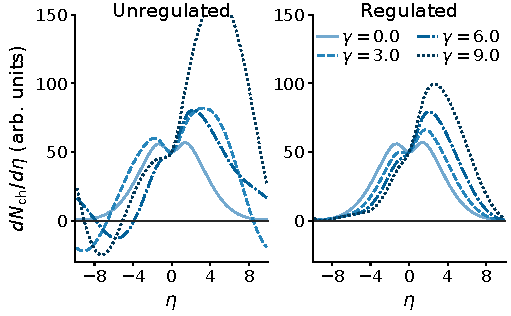
\includegraphics{regulate}
  \caption{Left: Unregulated skewness values lead to ill-behaved rapidity distributions. The distributions scale non-monotonically with skewness parameter $\gamma$ and go negative at large rapidities. Right: Replacing $\gamma$ by Eq.~\eqref{regulateEq} achieves desired monotonic scaling and suppresses negative regions.}
  \label{fig:regulate}
\end{figure}

\begin{figure}[b]
  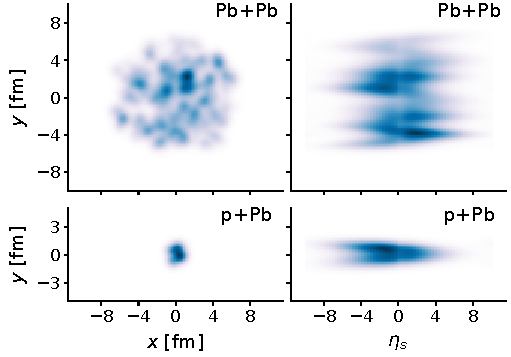
\includegraphics{trento3d_example}
  \caption{Initial entropy density in sample Pb+Pb (upper) and p+Pb (lower) events for cross sections of the $\eta=0$ and $x=0$ planes (left and right columns). Event is constructed using the relative skewness model in Table~\ref{tab:parametrization} with $\mu_0=1$, $\sigma_0=3$ and $\gamma_0=6$ along with midrapidity parameters from {Bernhard:2016tnd}.}
  \label{fig:3d-example}
\end{figure}

There is, however, a problem with the reconstructed function in Eq.~\eqref{gfunc}.
Rapidity distributions with large skewness are ill-behaved and oscillate to negative values for large $\eta$, as shown in the left panel of Fig.~\ref{fig:regulate}.
The conditions to ensure a positive definite Fourier transform are quite involved; instead, we employ the following substitution for $\gamma$ to regulate the distribution:
\begin{equation}
  \gamma \rightarrow \gamma \exp \left({-}\frac{1}{2}\sigma^2k^2 \right). \label{regulateEq}
\end{equation}
This leaves the skewness of the distribution intact while contributions from higher-order cumulants are included systematically.
The performance of the procedure depends on the domain of reconstruction.
For reasonable values of skewness, it is found to perform well within the range ${-3.3\, \sigma \le \eta \le 3.3\, \sigma}$.
Fig.~\ref{fig:regulate} shows the reconstructed function before and after the regulation procedure using four different skewness values.
The procedure strongly suppresses negative regions of charged particle density (in realistic calculations they are set to zero), and preserves a clear monotonic trend with increasing skewness.
The regulated generating function approach thus produces distributions which are both positive and well behaved over a wide range of rapidity and skewness.

In Fig.~\ref{fig:3d-example} we show the resulting entropy density $s(\x, \eta_s)$ produced by randomly generated Pb+Pb and p+Pb collisions (top and bottom panels respectively) using a set of typical parameter values, annotated in the figure caption.
The left column shows the entropy density at midrapidity $\eta_s=0$, while the right column shows a cross section of the entropy density in the plane defined by $x=0$.
We observe large entropy density fluctuations in the transverse plane arising from nucleon position fluctuations as well as significant forward-backward rapidity fluctuations which track the local asymmetry of projectile and target nucleon densities.
The event profiles---although not yet optimized---exhibit rich longitudinal structures which clearly break boost invariance.

At this point it is important to emphasize that the present entropy deposition parametrization is a purely \emph{local function} of nuclear overlap density.
In subsequent sections, we optimize the model parameters to fit \emph{global} pseudorapidity-dependent charged particle yields which have their transverse structure integrated out.
Obtaining quality fits to data thus remains a nontrivial task, as the model convolves a local entropy deposition mapping with a background distribution of fluctuating nuclear overlap density.

\section{Experimental observables}
The three-dimensional initial entropy profile and its longitudinal fluctuations directly relate to the average charged particle multiplicity and event-by-event fluctuations observed in the final state. 
The ALICE collaboration has published the centrality dependent pseudorapidity densities $\dnchdy$ in Pb+Pb collisions with a wide pseudorapidity coverage $-3.5<\eta<5.0$ {Abbas:2013bpa,ALICE:2015kda}, and the ATLAS collaboration has measured centrality-dependent $\dnchdy$ in p+Pb collisions within $|\eta| < 2.7$ {Aad:2015zza}.
However, such centrality binned $\dnchdy$ measurements only probe the initial entropy density averaged over many events. 
Information on the event-by-event fluctuations is carried by two-particle pseudorapidity correlation $C(\eta_1, \eta_2)$.
In particular, the long range contributions to the correlation function (LRC) are sensitive to the event-by-event initial state fluctuations and are ideal for examining stochastic properties of the three-dimensional initial conditions.

We follow {Bzdak:2012tp, Jia:2015jga, ATLAS:2015kla} and decompose the event-by-event charged particle pseudorapidity distribution within the acceptance $[-Y, Y]$ using normalized Legendre polynomials
\begin{align}
  \frac{dN}{d\eta} &= \biggl\langle\frac{dN}{d\eta}\biggr\rangle \biggl[1 + \sum_{n=0}^\infty a_n T_n\left(\frac{\eta}{Y}\right) \biggr], \\[.5ex]
  T_n(x) &= \sqrt{n + \frac{1}{2}}\, P_n(x).
\end{align}
The two-particle correlation function $C(\eta_1, \eta_2)$ is then calculated from the normalized multiplicity distribution $R(\eta) = dN/d\eta /\langle dN/d\eta\rangle$ and is decomposed into symmetrized polynomials $T_{mn}(\eta_1, \eta_2)$
\begin{align}
  C(\eta_1, \eta_2) &= \left\langle R(\eta_1) R(\eta_2)\right\rangle \\
  &= 1 + \sum_{m, n}\langle a_m a_n\rangle  T_{mn}(\eta_1, \eta_2),  \\
  T_{mn}(\eta_1, \eta_2) &= \frac{T_n(\eta_1)T_m(\eta_2) + T_m(\eta_1)T_n(\eta_2)}{2}.
\end{align}
Centrality fluctuations introduce nonzero $\langle a_0 a_n\rangle$ and are removed by renormalizing $C(\eta_1, \eta_2)$,
\begin{align}
  C_N(\eta_1, \eta_2) &= \frac{C(\eta_1, \eta_2)}{C_1(\eta_1)C_2(\eta_2)},\\[.5ex]
  C_{1,2}(\eta_{1,2}) &= \int_{-Y}^{Y}C(\eta_1, \eta_2)\frac{d\eta_{2,1}}{2Y}.
\end{align}
The forward-backward multiplicity fluctuations characterized by $\langle a_m a_n\rangle$ with $m, n > 0$ can then be projected out from the renormalized correlation function as
\begin{align}
  C_N(\eta_1, \eta_2) \sim 1 + \frac{3}{2}\langle a_1 ^2 \rangle \frac{\eta_1\eta_2}{Y^2} + \cdots.
\end{align}

The ATLAS collaboration has measured the centrality dependence of various $\langle a_m a_n\rangle$ in Pb+Pb collisions {ATLAS:2015kla, SoorajRadhakrishnanfortheATLAS:2015eqq} using particles with $p_T > 0.5$~GeV.
Recent theoretical work on these observables includes a longitudinal extension of IP-Glasma initial conditions {Schenke:2016ksl} and a rapidity-dependent constituent-quark MC-Glauber model which was embedded in three-dimensional hydrodynamic simulations {Denicol:2015bnf, Monnai:2015sca}.
It was shown that short range correlations (SRC) from resonance decays are a significant contribution to the $\langle a_m a_n\rangle$ signal, while variations in the transport coefficients have a much smaller effect {Denicol:2015bnf}.
The contributions from LRC and SRC were estimated in a subsequent ATLAS analysis {Jia:2016jlg} using correlations of same- and opposite-signed charged particles with $p_T > 0.2 \textrm{ GeV}$.
The isolated LRC, which were measured with a lower $p_T$ cut, are a cleaner observable for the study of initial state fluctuations, but they are not yet calculated for central Pb+Pb collisions.
We therefore perform the calculation {ATLAS:2015kla} with proper modeling of the SRC using the UrQMD model.

\section{Model-to-data comparison}

\begin{table}[t]
  \caption{Input parameter ranges for the rapidity-dependent parametric initial condition model.}

    \begin{tabular}{lll}
      Parameter & Description	& Range \\
      \paddedhline
      $N_{\textrm{p+Pb}}$    & Overall p+Pb normalization      & 140.0--190.0 \\
      $N_{\textrm{Pb+Pb}}$   & Overall Pb+Pb normalization     & 150.0--200.0  \\
      $p^\dagger$	                   & Generalized mean parameter      & -0.3--0.3  \\
      $k$	                   & Multiplicity fluct.\ shape      & 1.0--5.0  \\
      $w$	                   & Gaussian nucleon width     & 0.4--0.6  \\
      $\mu_0$                & Rapidity shift mean coeff.\     & 0.0--1.0  \\
      $\sigma_0$             & Rapidity width std.\ coeff.\    & 2.0--4.0  \\
      \multirow{2}{*}{$\gamma_0$}             & \multirow{2}{*}{Rapidity skewness coeff.\ }      & 0.0--10.0 (rel) \\
                  &        & 0.0--3.6 (abs)  \\
      $J$	                   & Pseudorapidity Jacobian param.  & 0.6--0.9
    \end{tabular}
   \raggedright{$\dagger$ Priori probability distributions fitted from {Bernhard:2016tnd} are applied on this parameter independently within the given ranges.}
  \label{tab:parameters}
\end{table}

The aforementioned rapidity extension introduces several new model parameters which necessitate rigorous optimization.
For this purpose, we apply established Bayesian methodology {OHagan:2006ba, Dave:pca, Higdon:2014tva, Wesolowski:2015fqa} to constrain the proposed parametric initial conditions and extract intrinsic, local features of the QGP fireball using macroscopic event-averaged quantities.
Ideally, one would run the full model calculation at each design point and calibrate the model to fit a comprehensive list of experimental measurements.

Unfortunately, three-dimensional viscous hydrodynamic simulations require an order of magnitude more computing resources than the boost-invariant models previously used in Bayesian analyses.
This makes it difficult to calibrate on statistically intensive observables such as multiparticle flow correlations which require tens of thousands of minimum bias events at each design point. 

Work is underway to solve these technical challenges by migrating three-dimensional viscous hydrodynamic simulations to graphics cards which offer dramatic performance enhancements over processors at a fraction of the cost {Bazow:2016yra}.
We instead omit higher order flow observables and calibrate only on the rapidity-dependent charged particle yields and two-particle pseudorapidity correlations which can be calculated with a few thousand events. 

It should also be noted that the data we use for Pb+Pb and p+Pb collisions are taken at different beam energies, ${\sqrts = 2.76}$~TeV and 5.02~TeV respectively.
Because phenomenological model parameters generally change with beam energy, it is not fully consistent to optimize a single set of parameters to fit experimental observables at two different energies.
Here we assume that all model parameters, except for the overall entropy normalizations, do not change drastically with the beam energy of the two datasets since the beam rapidity changes less than $8\%$ and perform a simultaneous multi-parameter fit using both measurements.

We now briefly summarize the procedure used to apply Bayesian methodology to the newly constructed parametric initial condition model. For a more comprehensive explanation see {Novak:2013bqa, Bernhard:2015hxa, Bernhard:2016tnd}. All steps are repeated for both the relative and absolute skewness models described in Table~\ref{tab:parametrization}.

\subsection{Parameter design}

The three-dimensional parametric initial conditions are specified using nine model parameters.
Five control entropy deposition at midrapidity:
\begin{itemize}[itemsep=0pt]
  \item[1--2.] two normalization factors for Pb+Pb and p+Pb collisions at $\sqrts=2.76$~TeV and 5.02~TeV beam energies,
  \item[3.] the generalized mean parameter $p$ which modulates entropy deposition at midrapidity,
  \item[4.] a gamma shape parameter $k$, which controls the variance of proton-proton multiplicity fluctuations,
  \item[5.] and a Gaussian nucleon width $w$, which determines initial state granularity;
\end{itemize}
the remaining four parameters add rapidity dependence to the model:
\begin{itemize}[itemsep=0pt]
  \setcounter{enumi}{6}
  \item[6--8.] three coefficients which modulate the local rapidity distribution's shift $\mu_0$, width $\sigma_0$, and skewness $\gamma_0$,
  \item[9.] and a Jacobian factor $J$ for the conversion from rapidity to pseudorapidity.
\end{itemize}

Given the large number of iterations required by multidimensional Monte Carlo optimization methods and the non-negligible computation time needed to sample initial condition events and evolve them through hydro, it is intractable to explore the aforementioned parameter space using direct model evaluation.
To circumvent this issue, we train emulators using a limited number of parameter configurations to reproduce the charged-particle pseudorapidity density and the two-particle pseudorapidity correlations predicted by evolving the initial condition model through hydrodynamics.
These emulators interpolate the predictions of the model between training points and provide essentially instant predictions at uncharted regions of parameter space.

The emulators are trained using 100 unique parameter configurations sampled from the parameter ranges listed in Table~\ref{tab:parameters}.
Each parameter design point is distributed in the nine dimensional space using a maximin Latin hypercube design---a space-filling algorithm that maximizes the minimum distance between pairs of points in the multidimensional space.

With the parameter design in hand, we run $4\times 10^3$ Pb+Pb and $10^4$ p+Pb initial condition events through hydrodynamics at each of the 100 points and calculate the charged-particle pseudorapidity density and two-particle pseudorapidity correlations.
The centrality bins are defined by charged particle multiplicity using the same kinematic cuts used by experiments: $|\eta|<0.8$ for Pb+Pb collisions and ${-4.9 < \eta < -3.1}$ for p+Pb collisions.
The resulting $\dnchdy$ and rms $a_1$ are concatenated to an observable array for each input parameter set.
Loosely speaking, the physics model maps the $m\times n$ parameter design matrix $X$ to an $m \times p$ observable matrix $Y$:
\begin{equation}
  \begin{pmatrix}
    x_{1,1} & \cdots & x_{1,n} \\
    \vdots  & \ddots & \vdots \\
    x_{m,1} & \cdots & x_{m,n} \\
  \end{pmatrix}
  \xrightarrow{\text{Model}}
  \begin{pmatrix}
    y_{1,1} & \cdots & y_{1,p} \\
    \vdots  & \ddots & \vdots \\
    y_{m,1} & \cdots & y_{m,p} \\
  \end{pmatrix},
  \label{design-obs}
\end{equation}
where $m=100$ is the number of design points, ${n=9}$ is the number of input parameters, and $p$ is the number of measured outputs.

\subsection{Model emulator}

Once the design matrix is specified and the model has been run at each design point to construct a corresponding observable matrix, we train a set of Gaussian process emulators to reproduce the predictions of the model.
A Gaussian process emulator is a powerful nonparametric regression method which can be used to interpolate a scalar function of one or more input parameters.
For example, given a set of multivalued inputs ${X=\{\x_1, \x_2, \ldots, \x_n\}}$, and a corresponding list of scalar outputs $\mathbf y=\{y_1, y_2, \ldots, y_n \}$, a Gaussian process emulator can be used to interpolate the function $f: \x \mapsto y$ subject to a pre-specified covariance function $\sigma(\x,\x')$.
We use an existing implementation of Gaussian process regression in this work {2014arXiv1403.6015A}.

Since Gaussian processes are fundamentally scalar functions, while our model produces vector outputs, we first transform the model outputs (normalized by experimental data) using principal component analysis.
The principal components $z$ are orthogonal, uncorrelated linear combinations of the original outputs and may be used to reduce the dimensionality of the output space, since the first several principal components often account for the majority of the model's variance {Dave:pca}.
Independent Gaussian processes are thus trained to emulate the first $q < p$ principal components of the centrality-dependent charged-particle pseudorapidity distribution for the two systems and the rms $a_1$ of Pb+Pb collisions separately.

We choose to include $q=6,$ $6,$ and $4$ principal components for $\dndyPP$,\, $\dndypP$ and rms $a_1$ which account for 99.5\% of the observed variance.
For the emulator covariance function $\sigma(\x, \x')$, we adopt a simple Gaussian form
\begin{equation}
  \sigma(\x, \x') = \sigma_\text{GP}^2 \exp\Biggl[ -\sum_{k=1}^n \frac{(x_k - x'_k)^2}{2\ell_k^2} \Biggr] + \sigma_n^2\delta_{\x\x'},
\end{equation}
which is well-suited for continuously differentiable, smoothly-varying models.
The variance of the Gaussian process $\sigma^2_\text{GP}$, correlation lengths $l_k$, and noise variance $\sigma_n^2$ are estimated from the model outputs by numerically maximizing the likelihood
\begin{equation}
  \log P = -\frac{1}{2}\mathbf y\trans \Sigma^{-1} \mathbf y - \frac{1}{2} \log | \Sigma | - \frac{m}{2} \log 2 \pi,
\end{equation}
where $\Sigma$ is the covariance matrix from applying the covariance function $\sigma$ to each pair of design points.

\begin{figure*}
  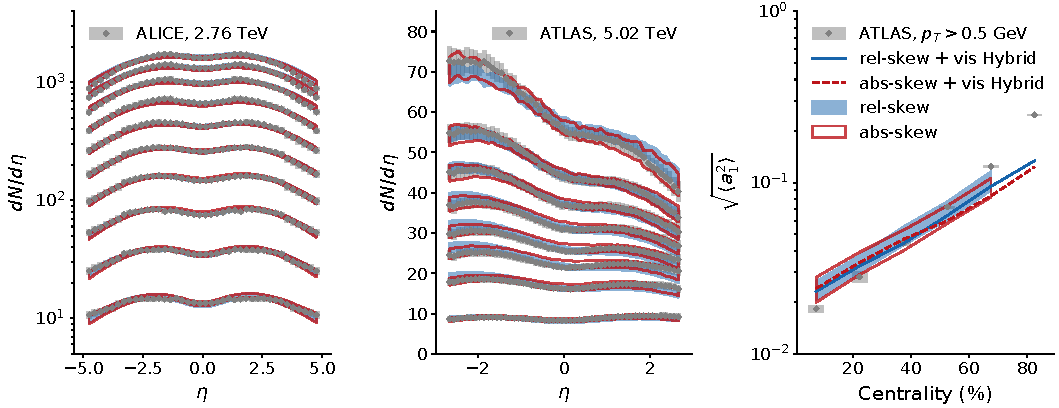
\includegraphics{post_obs}
  \caption{
  Left and Middle: Centrality and pseudorapidity dependence of the charged particle pseudorapidity density $\dndyPP$ at $\sqrts=2.76$~TeV and $\dndypP$ at $\sqrts=5.02$~TeV.
  Bands represents model emulator calculations $\dnchdy$ from the Bayesian posterior.
  Symbols are experimental data from ALICE {Abbas:2013bpa,ALICE:2015kda} and ATLAS {Aad:2015zza}.
  Rapidity cuts on model centrality selection are matched to experiment.
  Right: 
  The root-mean-square of the Legendre expansion coefficient $a_1$ estimated from two-particle pseudorapidity correlations plotted as a function of collision centrality.
 Bands represents model emulator calculations $\dnchdy$ from the Bayesian posterior, while lines are results from full event-by-event viscous hybrid model simulations using selected parameters from the Bayesian posterior.
  Symbols with errors are experimental data from ATLAS {SoorajRadhakrishnanfortheATLAS:2015eqq}.  
  }
  \label{fig:post_obs}
\end{figure*}
\subsection{Bayesian calibration and Bayes factor}

The parameter space of the emulated model is finally explored using Markov chain Monte Carlo (MCMC) methods.
The posterior probability for the \emph{true} model parameters $\x_\star$ is given by Bayes' theorem,
\begin{equation}
  P(\x_\star| X, Y, \y_\text{exp}) \propto P(X, Y, \y_\text{exp} | \x_\star) P(\x_\star).
  \label{bayes}
\end{equation}
The left-hand side is the Bayesian \emph{posterior}, the probability of true parameters $\x_\star$ given model design $X$, observable matrix $Y$, and experimental data $\y_\text{exp}$.
On the right, $P(X, Y, \y_\text{exp}| \x_\star)$ is the likelihood---the probability of observing $(X, Y, \y_\text{exp})$ given a proposal $\x_\star$---and $P(\x_\star)$ is the \emph{prior}, which encapsulates initial knowledge of $\x_\star$.

In this study, we place informative priors on the entropy deposition parameter $p$ using previous results at midrapidity.
Specifically, we set the priors on $p$ equal to the posterior distributions determined by the Bayesian analysis in Ref.~{Bernhard:2016tnd} which was calibrated to fit charged particle yields, mean transverse momenta, and flows at midrapidity.
For all remaining parameters, we assign a flat prior which is constant within the design range and zero outside.

We assume a Gaussian form for the likelihood function,
\begin{align}
  \begin{aligned}
  P &= P(X, Y, \y_\text{exp}|\x_\star) \\
    &= P(X, Z, \z_\text{exp}|\x_\star) \\
    &\propto\exp\biggl\{-\frac{1}{2}(\z_\star - \z_\text{exp})\trans \Sigma_z^{-1}(\z_\star - \z_\text{exp})\biggr\},
  \end{aligned}
  \label{eq:likelihood}
\end{align}
which is evaluated using the emulated principal components $\z_\star$ and transformed experimental data $\z_\text{exp}$.
Here $\Sigma_z$ is the covariance matrix for the principal components, which accounts for the various sources of uncertainty. We used a covariance matrix in the principal component space proportional to the identity matrix $\Sigma_z = \sigma I$, which corresponds to $5\%$, $10\%$, and $20\%$ relative error on the total variance of $\dndypP$,\, $\dndyPP$ and rms $a_1$.
This procedure effectively gives a larger weight to the p+Pb dataset, as it is more sensitive to the asymmetry parameters of the models, and it also emphasizes fitting single-particle observables over two-particle correlation observables.

Finally, the total log-likelihood of the model given by the p+Pb and Pb+Pb datasets is
\begin{align}\label{naive-formula}
\nonumber  \ln P &= \ln P_\text{pPb, $dN/d\eta$} + \ln P_\text{PbPb, $dN/d\eta$} \\
  &+  \ln P_\text{PbPb, rms $a_1$} + \ln P_{\text{priori}},
\end{align}
where $P_\text{piori}$ is the initial prior distribution.
The posterior is finally constructed by sampling the distribution using an affine-invariant MCMC sampler {emcee}.
In each MCMC step, the Gaussian process emulators first predict the principal components of the model outputs, the likelihood is then computed from Eq.~\eqref{eq:likelihood}, and the posterior probability is calculated from Bayes' theorem~\eqref{bayes}.
We use $\mathcal O(10^5)$ burn-in steps and $\mathcal O(10^6)$ production steps to generate the posterior distribution.

A model evaluation measure known as a Bayes factor can then be used to compare the performance of the relative- and absolute-skewness models.
It is defined as the ratio of the likelihood functions, integrated over each model's parameter space,
\begin{eqnarray}
	K = \frac{\int P(\textrm{Exp}|\textrm{Model I}, \vec{p}) d\vec{p}}{\int P(\textrm{Exp}|\textrm{Model II}, \vec{p}) d\vec{p}}\,.
\end{eqnarray}
The interpretation of the scale of $K$ is listed in Table \ref{tab:Kfactor}. {Jeffreys:1961}.
\begin{table}[t]
  \caption{Interpretation of the scale of $K$}
    \begin{tabular}{ll}
      K & Strength of evidence (supports model I) \\
      \paddedhline
      $ < 10^{1/2}$	& negative (supports model II)	\\
	  $10^0$ -- $10^{1/2}$	& barely worth mentioning	\\
	  $10^{1/2}$ -- $10^1$	& substantial	\\
	  $10^1$ -- $10^{3/2}$	& strong	\\
	  $10^{3/2}$ -- $10^2$	& very strong	\\
	  $>10^2$	& decisive	\\
    \end{tabular}
  \label{tab:Kfactor}
\end{table}
With $K<1$, the experimental data supports model II; while increasing $K$ above $1$, model I is supported with increasing strength of evidence.



\section{Calibration results}
\subsection{Calibrated observables}
To investigate the performance of the calibrated models, we show in Fig.~\ref{fig:post_obs} the resulting observables calculated from each model's calibrated emulators.
The bands are centered around the mean prediction, and their spread denotes $\pm 2$ standard deviations.
Both calibrated models are able to simultaneously describe $\dnchdy$ for the two collision systems as functions of rapidity and centrality, illustrating the flexibility of the generating function approach.

The results for rms $a_1$ are compared to preliminary data from ATLAS {ATLAS:2015kla} in Fig.~\ref{fig:post_obs}.
Both models capture the increasing trend of rms $a_1$ as function of centrality.
Hybrid model calculations agree with experimental measurements within $20\%$ for $0$--$50\%$ centralities ($N_{\textrm{part}} \gtrsim 75$) but underestimate the data at more peripheral centralities.
We notice that in {ATLAS:2015kla}, \mbox{HIJING} calculations reproduce rms $a_1$ for $N_{\textrm{part}} \lesssim 80$ but overpredict the signal at larger $N_{\textrm{part}}$.
This suggests that hydrodynamic calculations and microscopic models are complementary in understanding longitudinal fluctuations.

Averaging the likelihood function over an ensemble of posterior parameter sets for each model gives the model likelihood, from which the Bayes factor is calculated,
\begin{eqnarray}
K = \frac{\text{Relative-skewness model}}{\text{Absolute-skewness model}} = 2.5 \pm 0.2. 
\end{eqnarray}
This value is too close to unity to make a decisive statement regarding the preference of one model over the other {Jeffreys:1961}.
Indeed, the absolute-skewness model is slightly better in capturing the asymmetries in p+Pb collisions; while the relative-skewness model exhibits a larger curvature for rms $a_1$, closer to experiment.
This is not a surprise since these two models give effectively the same local entropy profile as shown in the previous subsection.

In summary, both models describe the p+Pb and Pb+Pb charged-particle pseudorapidity densities in all centrality bins to 10\% accuracy.
It also describes the rms $a_1$ from central to mid-central Pb+Pb collisions.
Both models fail to describe the rms $a_1$ in peripheral collisions which suggests that additional sources of fluctuation are needed in addition to nuclear thickness function fluctuations.
Relevant sources could include initial dynamical fluctuations such as string fragmentation, subnucleonic fluctuations, and finite-particle effects.

\begin{figure*}
  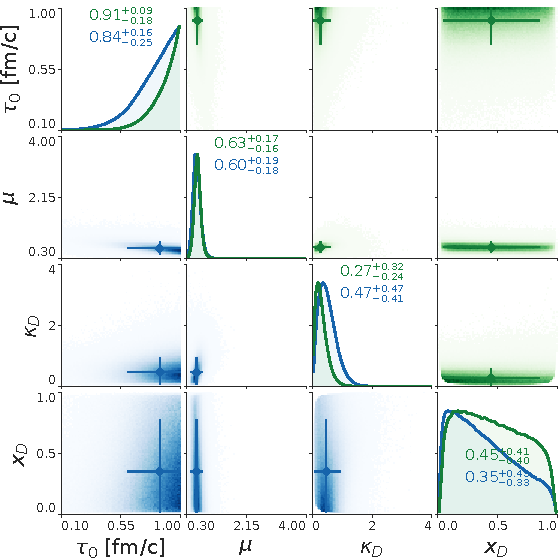
\includegraphics{posterior}
  \caption{Posterior distributions of the model parameters, listed in Table~\ref{tab:parameters}, for the relative-skewness (blue lower diagonal) and absolute-skewness (red upper diagonal) models. The diagonal panels are the marginal likelihood distributions of individual model parameters, while off-diagonal panels are joint distributions for pairs of model parameters.}
  \label{fig:posterior}
\end{figure*}

\subsection{Posterior distribution of model parameters}
Fig.~\ref{fig:posterior} presents the Bayesian posterior probability distributions for the relative- and absolute-skewness models (blue lower- and red upper-triangular matrices respectively).
Diagonal panels show the marginal posterior distribution of individual model parameters (all other parameters integrated out), while off-diagonal panels show the joint distribution for pairs of model parameters, reflecting their correlations.

The posterior distributions contain a wealth of information; here we summarize a few key observations:
\begin{itemize}[itemsep=0pt, leftmargin=2\parindent]
  \item Both models prefer the entropy deposition parameter $p$ close to $0$, consistent within the range of the prior distribution extracted from {Bernhard:2016tnd}.
  \item The p+p multiplicity fluctuation parameter is well constrained and distributed about $k=2.0$ for both models.
    These $k$ values are also consistent with the range of the previous estimates obtained from fits to p+p, p+Pb, and Pb+Pb multiplicity distributions at midrapidity {Moreland:2014oya}.
  \item The relative-skewness model prefers a larger nucleon width than the absolute-skewness model. 
  For future studies, one may also use more granular protons with subnucleonic structure instead of Gaussian protons.
  \item The calibrated relative-skewness model exhibits almost zero shift about the mean and large skewness, while the absolute-skewness model prefers a shift close to the center-of-mass rapidity and a moderate skewness. 
\end{itemize}
Superficially, it appears that the models prefer qualitatively different mechanisms for longitudinal entropy deposition; however, for realistic values of the nuclear thickness function in heavy-ion collisions, the behavior of the two calibrated models is nearly identical, despite the use of two possible skewness parametrizations, as is shown in Fig.~\ref{fig:post_dsdy}.
The lines and bands in Fig.~\ref{fig:post_dsdy} correspond to the mean and $1\sigma$ uncertainty of the calibrated models predictions. 
We vary the nuclear thickness functions $T_A$ and $T_B$ from $0.2~\text{fm}^{-2}$ to $2.6~\text{fm}^{-2}$. The maximum of the nuclear thickness function for a Pb nucleus in an optical Glauber model is about $2.2~\text{fm}^{-2}$. However, the event-by-event $T_A$ and $T_B$ may exceed this value in the presence of nucleonic fluctuations.
The calibrated relative- and absolute-model predictions agree within $1\sigma$ uncertainty band.
This observation has an important implication.
The two models adapt their parameters independently to describe the data and they coincide on one functional form of initial entropy deposition in terms of $T_A$ and $T_B$.
Therefore, with experimental inputs from the charged particle pseudorapidity densities and two-particle pseudorapidity correlations, a systematic model-to-data comparison can extract the form of the three-dimensional initial entropy distribution for relativistic heavy-ion collisions at the LHC.

\begin{figure}
  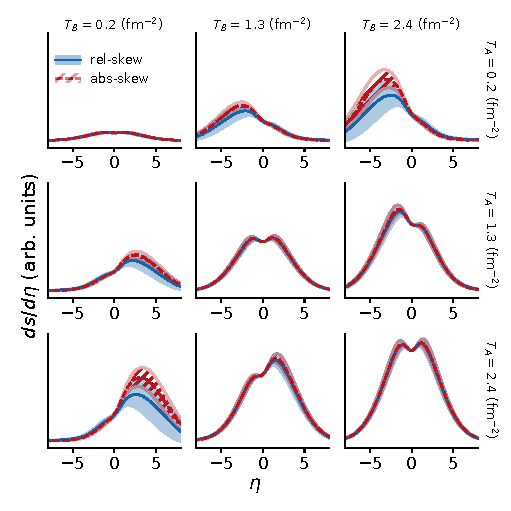
\includegraphics{post_dsdy}
  \caption{Applying parameters sampled from the posterior probability distribution to Eq.~\eqref{cgf} along with Eq.~\eqref{regulateEq}, this plot shows the resulting local entropy profile $ds/d\eta$ varying $T_A$ and $T_B$ from $0.2~\text{fm}^{-2}$ to $2.6~\text{fm}^{-2}$. The lines are the mean predictions and the bands denote $1\sigma$ model uncertainties.
  }
  \label{fig:post_dsdy}
\end{figure}


\section{Predictions for novel observables}
Both the relative- and absolute-skewness models provide comparable descriptions of multiplicity observables in p+Pb and Pb+Pb collisions which makes sense given that they predict effectively identical three-dimensional initial entropy profiles when calibrated to fit experimental data.
In this section, we proceed to investigate whether they can describe azimuthally sensitive observables such as flows, event-plane decorrelations and symmetric cumulants, and for completeness, we shall conduct the calculation with both models.
Here we use selected initial condition parameters around the peaks of the posterior distributions for each model (Table \ref{tab:chosen_parameters}) and perform viscous 3+1D hydrodynamic evolution with UrQMD as an afterburner.
These observables are a nontrivial test of the proposed model as they resolve azimuthal correlations which have not been included in the calibration process.

\begin{table}[t]
  \caption{Selected high-probability parameter sets}
    \begin{tabular}{lll}
      Parameter & rel-skew	& abs-skew \\
      \paddedhline
      $N_{\textrm{Pb+Pb}}^\dagger$   & 150.0     & 154.0  \\
      $p$	    & 0.0      & 0.0  \\
      $k$	    & 2.0     & 2.0  \\
      $w$	    & 0.59     & 0.42  \\
      $\mu_0$   & 0.0     & 0.75  \\
      $\sigma_0$ & 2.9    & 2.9  \\
   	  $\gamma_0$ & 7.3		& 1.0	\\
      $J$	     & 0.75 & 0.75	\\
    \end{tabular}
  \raggedright{$\dagger$ Normalization tuned with ideal hydro is reduced when using viscous hydro.}
  \label{tab:chosen_parameters}
\end{table}

\subsection{Anisotropic flows} 
As a preliminary check, we first verify that previous results for the elliptic and triangular flow harmonics $v_2\{2\}$ and $v_3\{2\}$ obtained using \trento\ initial conditions at midrapidity {Bernhard:2016tnd} are indeed recovered by the rapidity-dependent model extension.
Fig.~\ref{fig:vn_cen} shows the centrality dependence of $p_T$-integrated flow for ${0.2  < p_T < 5.0}$~GeV and $|\eta| < 0.8$ calculated from the \emph{three-dimensional} hybrid model compared to \mbox{ALICE} measurements {Adam:2016izf} using the  $Q$-cumulant method {Bilandzic:2010jr}.
The 3+1D hydrodynamics code used in this study only partially implements bulk viscous corrections and thus is not yet suitable for quantitative calculations involving finite bulk viscosity.
We therefore assert a QGP specific bulk viscosity $\zeta/s = 0$ which precludes direct comparison with the boost-invariant VISH2+1 hydrodynamics code {Song:2007ux, Shen:2014vra, Bernhard:2016tnd} and the corresponding shear and bulk viscosities determined by the previous Bayesian analysis {Bernhard:2016tnd}.
For the QGP specific shear viscosity, we choose constant QGP $\eta/s = 0.17$ and $0.19$ for relative- and absolute-skewness models respectively, which provide good descriptions of the data {Gale:2012rq, Niemi:2015qia}, although it is not a systematic best fit.
The resulting $v_2\{2\}$ and $v_3\{2\}$ agree with experimental data within $10\%$ and verify that the generating function rapidity extension recovers previous \trento\ initial condition results at midrapidity.

\begin{figure}
  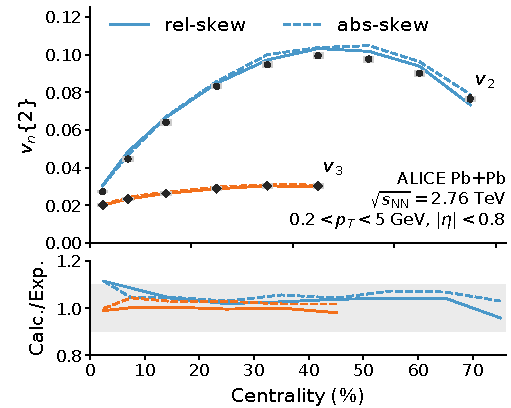
\includegraphics{vn_cen}
  \caption{Elliptic and triangular flow cumulants $v_2\{2\}$ and $v_3\{2\}$ as a function of centrality calculated from 3+1D hybrid model simulations using constant specific shear viscosity $\eta/s=0.17$ and $0.19$ for relative- and absolute-skewness models respectively, zero bulk viscosity $\zeta/s=0$ and hydro-to-micro switching temperature $T_\text{sw}=154$~MeV.
  The initial condition parameters are selected from the Bayesian posterior.}
  \label{fig:vn_cen}
\end{figure}

We now proceed to calculate the pseudorapidity-dependent flows which provide a sensitive handle on the QGP transverse structure at different rapidity values.
The ALICE collaboration has measured $v_n\{2\}(\eta)$ and $v_2\{4\}(\eta)$ within the wide pseudorapidity interval $-3.5 < \eta < 5.0$ and extrapolated to zero $p_T$ {Adam:2016ows}. 
This extrapolation reduces integrated flow relative to measurements with a nonzero $p_T$ cut because it averages over low-$p_T$ particles which generally have less flow.
The same behavior occurs in hydrodynamic models, although models which mispredict mean $p_T$ also mispredict the corresponding change in flow produced by introducing a $p_T$ cut.
The hybrid model used in this study omits bulk viscous corrections and thus overpredicts mean $p_T$.
This means it cannot describe hydrodynamic flow measurements with different $p_T$ cuts using a single value of $\eta/s$.
To circumvent this issue, we use $\eta/s=0.25$--$0.28$ when comparing to ALICE measurements that are extrapolated to zero $p_T$. 
Future implementation of realistic bulk viscous corrections would eliminate such fine tuning.

The pseudorapidity-dependent flows are estimated using the cumulant approach {Bilandzic:2010jr}, where particles of interests (POI) are correlated with reference particles.
The differential flow is then calculated via,
\begin{eqnarray}
v_n^\prime\{2\} = \frac{d_n\{2\}}{\sqrt{c_n\{2\}}},\\
v_n^\prime\{4\} = \frac{-d_n\{4\}}{\left(-c_n\{4\}\right)^{3/4}},
\end{eqnarray}
where $d_n\{2\}$, $d_n\{4\}$ is the two- and four-particle cumulants between the POI and reference particles and $c_n\{2\}$ and $c_2\{4\}$ are the cumulants among reference particles.
For POI with $\eta > 0$ ($\eta < 0$), the reference particles are restricted to $-0.8 <\eta < 0$ ($0 <\eta < 0.8$) to avoid autocorrelations.
The results are shown in the left panel of Fig.~\ref{fig:vn_eta} for nine centrality classes.
The correlation functions $d_n(\eta)$ and $c_n(\eta)$ are symmetrized since the event-averaged pseudorapidity-differential flow for the Pb+Pb system should be invariant with respect to the substitution $\eta \rightarrow -\eta$.

Both models predict $v_2\{2\}$, $v_2\{4\}$ and $v_3\{2\}$ that decrease from mid to forward/backward rapidity and produce a triangle shaped structure as measured by ALICE.
Incidentally, the absolute-skewness model agrees with experiment slightly better at large pseudorapidity.
It has been realized that the slope of $v_n(\eta)$ which produces this triangular shape is highly sensitive to the hadronic shear viscosity {Denicol:2015bnf}, and thus Fig.~\ref{fig:vn_eta} corroborates that UrQMD provides a semi-quantitative description of hadronic viscosity below the QGP transition temperature.
However, for central to mid-central collisions, the slope of the decreasing $v_2$ as a function of pseudorapidity is underpredicted, resulting in a flatter $v_n(\eta)$ than the experiments.
The reason for this discrepancy may be complicated.
Apart from improving initial conditions, a realistic bulk viscosity and a temperature dependent specific shear viscosity should definitely affect the results.
Another reason could be the use of the QCD EoS and QGP transport coefficient $\eta/s$ in the limit of vanishing baryon chemical potential, which may not be a good approximation at large pseudorapidity even at LHC energies.

\begin{figure*}
  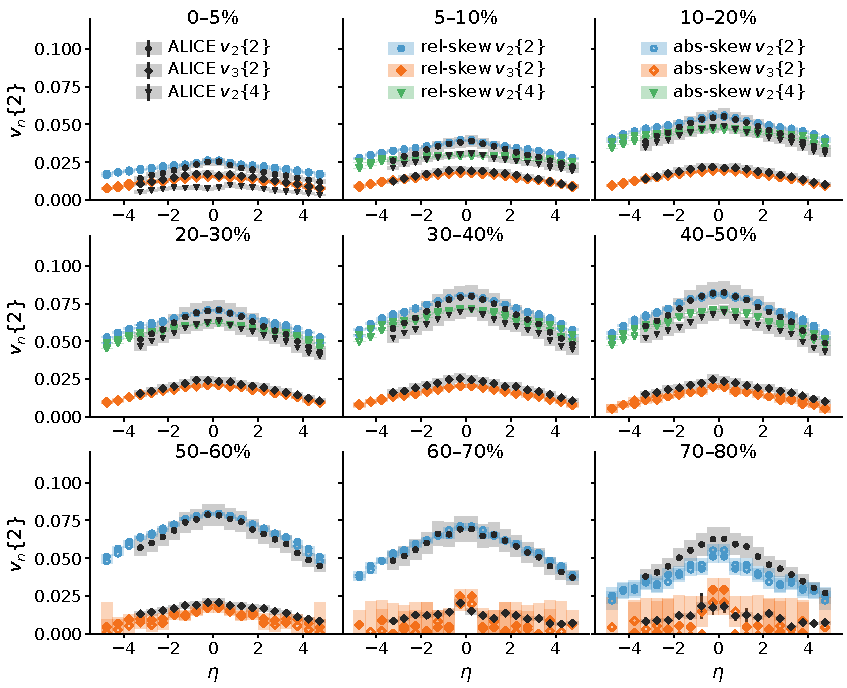
\includegraphics{vn_eta}
  \caption{Pseudorapidity dependence of anisotropic flow coefficients $v_2\{2\}$, $v_3\{2\}$ and $v_2\{4\}$ (blue circle, green triangle and orange diamond shaped symbols) calculated from the hybrid model with constant specific shear viscosity $\eta/s=0.25$ and $0.28$ for relative- and absolute-skewness models respectively (solid and open symbols), compared to data from ALICE (smaller black symbols) with $p_T > 0$~GeV (extrapolated) in different centrality bins. 
  The bands for each theory calculation point indicate $1\sigma$ statistical error, while experimental bands/bars denote $1\sigma$ systematic and statistical errors respectively.}
  \label{fig:vn_eta}
\end{figure*}



\begin{figure*}
  \begin{center}
  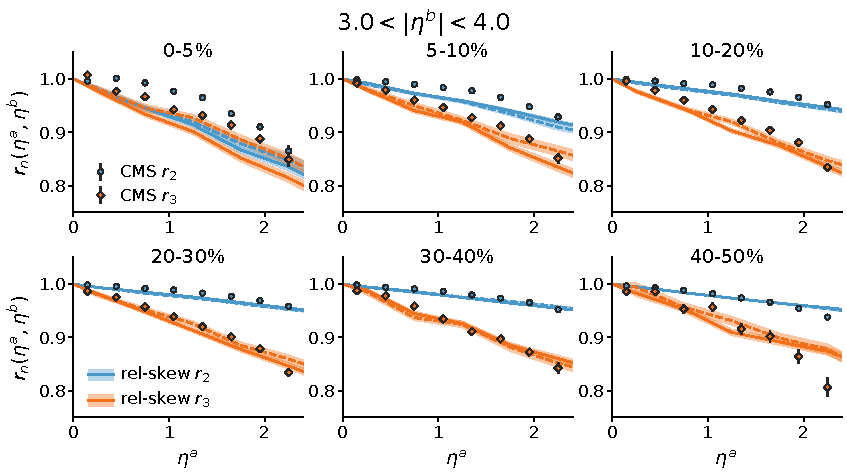
\includegraphics{evt_pln_decorr_near}
  \quad\quad\quad
  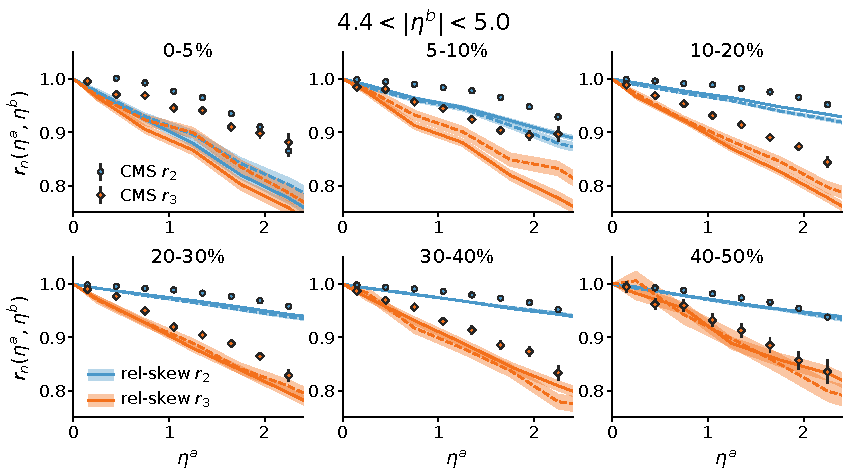
\includegraphics{evt_pln_decorr_far}
  \end{center}
  \caption{Left: The event-plane decorrelation for $n=2,3$ in different centrality bins with the reference particles from $3.0<|\eta^b|<4.0$.
  Right: The same quantities as the left panel but with the reference particles from $4.4<|\eta^b|<5.0$. 
  Theory bands indicate $1\sigma$ statistical error, while experimental bands/bars denote $1\sigma$ systematic and statistical errors respectively.}
  \label{fig:epd}
\end{figure*}


\subsection{Event-plane decorrelation}

Next, we study the event-plane decorrelation as a function of pseudorapidity using the calibrated relative-skewness model. 
The event planes are defined by the angles
\begin{equation}
  \Psi_n^\text{EP} = \frac{\text{atan2}(\langle \sin n \phi \rangle, \langle\cos n \phi \rangle)}{n},
\end{equation}
where the average is performed over particles of interest.
In general, the angles $\Psi_n^\text{EP}$ may change as a function of pseudorapidity due to longitudinal initial state fluctuations and finite particle effects.
As a consequence, two event-plane angles constructed from sets of particles separated by a finite rapidity gap will decorrelate as the rapidity gap increases.
This effect is important as it affects not only the calculation of soft observables involving a finite pseudorapidity gap or a large pseudorapidity interval, but also the interpretation of hard probe observables where particles from a rare hard process are often correlated with reference particles from different pseudorapidity bins.
It has been studied in a number of previous works including a longitudinally torqued fireball model with fluctuating sources {Bozek:2015bna}, AMPT calculations which studied its influence on flow observables {Jia:2014ysa, Xiao:2012uw}, as well as coarse-grained AMPT initial conditions that were embedded in 3+1D ideal hydrodynamic simulations {Pang:2015zrq}.

The decorrelations receive contributions from both random fluctuations during the evolution process and the systemic twist of the participant plane arising from initial longitudinal fluctuations {Bozek:2015bna}.
In the present parametric initial condition model, the participant plane twist arises naturally from local longitudinal fluctuations.
The transverse geometry at forward (backward) space-time rapidity is dominated by the projectile (target) participant density.
As a result, the participant plane gradually interpolates between the projectile and target densities, leading to a systemic twist in the beam direction.
The time evolution also contributes to decorrelation among the event-planes.
For example, early- and late-stage dynamics introduce additional fluctuations that partially randomize event-plane orientations.
Stochastic contributions from pre-equilibrium dynamics are neglected in the present study, but fluctuations in the hadronic phase are naturally accounted for by the UrQMD transport model.

The CMS collaboration has measured the event-plane decorrelations in Pb+Pb collisions using the $\eta$-dependent factorization ratio $r_n(\eta^a, \eta^b)$ {Khachatryan:2015oea}, defined as
\begin{align}
  r_n(\eta^a, \eta^b) &= \frac{V_{n\Delta}(-\eta^a, \eta^b)}{V_{n\Delta}(\eta^a, \eta^b)}, \\
  V_{n\Delta}(\eta^a, \eta^b) &= \langle\langle \cos(n\Delta\phi) \rangle\rangle,
\end{align}
where the double average means averaging over particles in each event and then averaging over all events in a given centrality class. 
The use of three $\eta$-bins ($\pm \eta^a$ and $\eta^b$) reduces short range correlations.
The ratio $r_n(\eta^a, \eta^b)$ reflects the fluctuation of event-plane angles separated by $\eta^a+\eta^b$ relative to the fluctuation of angles separated by  $|\eta^a-\eta^b|$ {Khachatryan:2015oea}.

We compare our calculation to the CMS measurements with both $3.0 < \eta^b < 4.0$ and $4.4 < \eta^b < 5.0$ and momentum cuts $p_T^b > 0$~GeV and ${0.3 < p_T^a < 3.0}$~GeV.
The $\eta$-dependent factorization ratios $r_2$ and $r_3$ for six centrality classes and different $\eta^b$ cuts are shown in Fig.~\ref{fig:epd}.
Both models predict a prominent $n=2, 3$ event-plane decorrelation in central collisions which decreases with increasing centrality.
For midcentral collisions, the nuclear geometry largely defines the $n=2$ participant plane---fluctuations and twisting are perturbations around this predominant direction---and hence $r=2$ decorrelation is reduced.
On the other hand, the $n=3$ event-plane receives little contribution from the nuclear geometry but is dominated mostly by fluctuations; it therefore has a similar slope over all six centralities.
In central collisions, the contribution from nuclear geometry is overwhelmed by fluctuations leading to similar $n=2$ and $n=3$ decorrelations.
The calculations describe the observed $n=2,3$ event-plane decorrelations with $3.0 < \eta^b < 4.0$ very well except the most central $0$--$5\%$ centrality, but systematically overpredict the magnitude of the decorrelations with $4.4 < \eta^b < 5.0$, especially for $0$--$10\%$ central collisions.
The reason is that the model, by construction, extends well-developed mid-rapidity initial conditions to finite pseudorapidity. 
Even though it is calibrated to multiplicity observables, it gradually loses its predictive power for fine-structure flow observables when moving far away from mid-rapidity.
Specifically, the model predicts decorrelations between the event-planes that are stronger for larger $\eta^b$ bins, while the experiment sees that the magnitude of decorrelation saturates when moving from $3.0<\eta^b<4.0$ to $4.4<\eta^b<5.0$.
Future improvements to the model at large pseudorapidity are clearly needed.
Nevertheless, the model's explanation of the event-plane decorrelations for $3.0 < \eta^b < 4.0$ remains nontrivial.
Both models were both calibrated with $\dnchdy$ and rms $a_1$ data.
These multiplicity observables do not constrain the transverse structure of the event at different pseudorapidities, and hence reproducing $r_2$ and $r_3$ means the calibrated initial condition models not only reproduce global longitudinal entropy deposition and fluctuations, but also capture features of the longitudinal dependence of transverse geometry within $|\eta| \lesssim 4$.


\begin{figure*}
  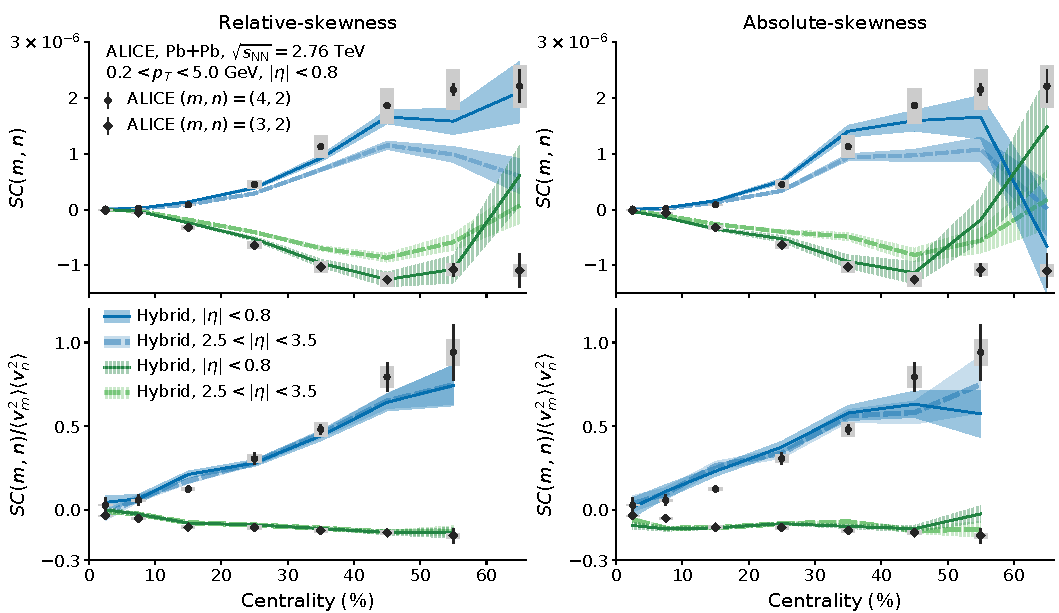
\includegraphics{smn}
  \caption{Top row: calculated $SC(4,2)$ and $SC(3,2)$ as functions of centrality compared to ALICE measurements, with the same 3D hybrid model set-up as used for Fig. \ref{fig:vn_cen}.
  We conduct calculations in two kinematic ranges: $|\eta|<0.8$ is the pseudorapidity cut used by current the ALICE measurement and $2.5<|\eta|<3.5$ is our prediction for the symmetric cumulants away from mid-rapidity in the Pb+Pb system.
  Bottom row: $SC(m,n)$ normalized by $\langle v_m^2\rangle\langle v_n^2\rangle$ for two two kinematic ranges.
  The left column and right column show results using relative- and absolute-skewness respectively.
   }
  \label{fig:smn} 
\end{figure*}


\subsection{Flow correlations}

Correlations between different anisotropic flow harmonics can be used to further constrain the initial state geometry {Niemi:2012aj}.
Experimentally, these correlations can be quantified using either event shape engineering {Schukraft:2012ah, Aad:2015lwa} or the symmetric cumulants $SC(m,n)$ {Bilandzic:2013kga}. 
Here we focus on the symmetric cumulants which are defined as,
\begin{align}
SC(m, n) &= \langle\langle \cos(m\phi_1+n\phi_2-m\phi_3-n\phi_4)\rangle\rangle \nonumber \\
\nonumber &- \langle\langle\cos[m(\phi_1-\phi_2)]\rangle\rangle\langle\langle\cos[n(\phi_1-\phi_2)]\rangle\rangle \label{eq:scmn}\\
&= \langle v_m^2 v_n^2 \rangle - \langle v_m^2\rangle\langle v_n^2\rangle.
\end{align}
The centrality dependences of $SC(4,2)$ and $ SC(3,2)$ at midrapidity have recently been measured by ALICE {ALICE:2016kpq}. 
A positive value of $SC(m,n)$ means that a large $v_m$ is more likely to be observed with a large $v_n$, while for negative values of $SC(m,n)$, a large $v_m$ favors small $v_n$.
The symmetric cumulants $SC(m,n)$ are nearly insensitive to nonflow effects while remaining sensitive to collective effects, initial geometry fluctuations $\langle \varepsilon_m^2 \varepsilon_n^2 \rangle - \langle \varepsilon_m^2 \rangle \langle \varepsilon_n^2 \rangle$ and the QGP specific shear viscosity {ALICE:2016kpq, Zhu:2016puf}.
To remove its dependence on the magnitudes of $\langle v_m^2\rangle$ and $\langle v_n^2\rangle$, we also calculate the normalized symmetric cumulants
\begin{equation}
  NSC(m,n) = SC(m,n)/\langle v_m^2\rangle\langle v_n^2\rangle.
\end{equation}
Here we use this tool to not only study the flow correlations at midrapidity, but also reveal its pseudorapidity dependence.

Fig.~\ref{fig:smn} shows the calculated symmetric cumulants compared to ALICE measurements using the relative- and absolute-skewness models with the same transport coefficients as in Fig.~\ref{fig:vn_cen}. 
We use the same centrality bins as ALICE experiments and the centrality averaged symmetric cumulants are performed with a multiplicity weight as discussed in {Gardim:2016nrr}.
We first calculate $SC(4,2)$ and $SC(3,2)$ at midrapidity $|\eta|<0.8$ (solid lines) to match the rapidity cuts of the ALICE measurement.
The negative $SC(3,2)$ is a result of initial eccentricity correlations, while the large positive $SC(4,2)$ is produced by nonlinear correlations between $v_2$ and $v_4$ during the medium evolution {Giacalone:2016afq, Qian:2016fpi, Bhalerao:2014xra, Zhou:2015eya}.
The resulting symmetric and normalized symmetric cumulants agree with the data quite well and support previous constraints on the QGP initial conditions at midrapidity {Bernhard:2016tnd}. 

Next, we shift our attention away from midrapidity and predict the symmetric (normalized symmetric) cumulants in the rapidity interval $2.5 < |\eta| < 3.5$ (dashed lines) which has not been measured.
In this calculation, we take two reference particles from $|\eta| < 0.8$ and two POI from $2.5 < |\eta| < 3.5$ and calculate
\begin{align}
SC^\prime(m, n) &= \langle\langle \cos(m\phi_1+n\phi_2-m\phi_3^\prime-n\phi_4^\prime)\rangle\rangle \\
\nonumber &- \langle\langle\cos[m(\phi_1-\phi_2^\prime)]\rangle\rangle\langle\langle\cos[n(\phi_1-\phi_2^\prime)]\rangle\rangle, \label{eq:scmn}
\end{align}
where the primed symbols represents the azimuthal angle of POI.
Magnitudes of both $SC^\prime(4, 2)$ and $SC^\prime(3, 2)$ are significantly suppressed at forward/backward rapidities, in accordance with the behavior of $v_2\{2\}(\eta)$ and $v_3\{2\}(\eta)$ as presented in the text in Fig.~\ref{fig:vn_eta}.
However the normalized symmetric cumulants $NSC^\prime(4,2)$ and $NSC^\prime(3,2)$ are consistent within uncertainty bands for different pseudorapidity cuts.
We observe that the normalized symmetric cumulant does not change as a function of psuedorapidity for either the relative- or absolute-skewness model and hence expect it to remain constant in nature as well.
Future comparison with available data should correspondingly impose strong constraints on our approach for modeling the three-dimensional initial conditions.


\section{Conclusion}

In summary, we have proposed a new method to extend arbitrary initial condition models defined at midrapidity to forward and backward pseudorapidity.
The method describes initial entropy deposition as a purely local function of nuclear participant densities, with the longitudinal profile reconstructed from generating-function cumulants.
The first three cumulants of the distribution (mean, standard deviation, and skewness) are included.
We set the mean proportional to the center-of-mass rapidity of local nuclear participant densities, and parametrize the standard deviation using a constant rapidity width.
Two models for the distribution's skewness are investigated: one where the skewness is proportional to the relative nuclear thickness difference, and one where it is proportional to the absolute difference.

We apply the method to extend the parametric \trento\ initial condition model which has been previously used to constrain QGP initial conditions and medium properties at midrapidity. 
The resulting three-dimensional models are then calibrated using Bayesian parameter estimation to fit p+Pb and Pb+Pb charged particle pseudorapidity densities $\dnchdy$ and the root-mean-square of the two particle pseudo-rapidity correlation's Legendre decomposition coefficient $a_1$ at the LHC.
After the calibration, both models provide comparable descriptions of experimental $\dnchdy$ and rms $a_1$ data.
Despite the apparent difference in the skewness ansatz, the calibrated models predict effectively the same behavior for local longitudinal entropy deposition as function of nuclear thickness in heavy-ion collisions.

Using the calibrated relative- and absolute-skewness initial condition models, we study pseudorapidity-dependent anisotropic flows, event-plane decorrelations and flow correlations in Pb+Pb collisions.
The model nicely describes integrated flows $v_2$ and $v_3$ at midrapidity as well as the pseudorapidity dependence of differential flow for different centrality classes.
The elliptic and triangular event-plane decorrelations with $3.0 < |\eta^b| < 4.0$ are well explained except for the most central collisions, but both models overpredict the decorrelations with the reference particles $4.4 < |\eta^b| < 5.0$.
This is because the model is an extension from mid-rapidity calculation and it gradually loses its accuracy at large forward/backward rapidity.
Both models give a satisfactory description of flow correlation $SC(3,2)$ and $SC(4,2)$ at midrapidity, which can be used to predict their values at forward/backward pseudorapidity where their values have not yet been measured.

The present work expands upon previous efforts to parametrize and constrain local initial condition properties using global final-state observables.
We show that these local properties are overconstrained by multiplicity observables alone and can be reverse engineered using systematic model-to-data comparison with quantitative uncertainty.
Specifically, it is a first attempt to use data-driven methods to infer what the entropy density distribution looks like at the hydrodynamic starting time in all three spatial dimensions.

It is clear that local forward/backward fluctuations are responsible for a variety of longitudinally sensitive phenomena beyond mere multiplicity fluctuations.
The general agreement of the present framework with pseudorapidity dependent flows and event-plane decorrelations corroborates the use of relativistic viscous hydrodynamics in describing the QGP dynamics away from midrapidity region.
The resulting knowledge can then be used to provide direct feedback for first-principle calculations of the QGP initial conditions, and can also be applied to studies where the QGP initial conditions act as a nuissance parameter, e.g.\ when modeling the propagation of hard probes through the medium in order to measure their response.

The present analysis would benefit from a number of future improvements.
For example, it would be interesting to add subnucleonic structure to the nuclear thickness functions in order to examine its effect on longitudinal rapidity fluctuations.
Also, in this work we assume that the multiplicity observables are insensitive to viscous effects and use ideal hydrodynamics in the model-to-data comparison process.
In the calculation of flow observables, we use an over-simplified constant specific shear viscosity and zero bulk viscosity, although there have been many works suggesting preference for a temperature dependent shear viscosity and finite bulk viscosity {Bernhard:2016tnd,Niemi:2015qia, Ryu:2015vwa}.
We leave these refinements to future work and hope the calibrated initial conditions presented in this study provide a more realistic description of the three-dimensional structure of relativistic heavy-ion collisions which will prove useful in constraining the properties of hot and dense QCD matter.


\section{Hybrid model simulation}\label{app}

The 3+1D relativistic viscous hydrodynamics code \mbox{vHLLE} {Karpenko:2013wva} is used for the QGP medium evolution. 
The equation-of-state (EoS) is obtained by interpolating a state-of-the-art lattice-QCD EoS {Bazavov:2014pvz} at high temperature with vanishing baryon density and a hadron resonance gas EoS at low temperature.
We use a switching energy density $\varepsilon_s = 0.322$~GeV/fm$^3$ ($T_s\sim0.154$~GeV) at which the hydrodynamic description is switched to the UrQMD transport description. 
The switching temperature $T_s$ is the same as the EoS pseudo-critical temperature $T_c = 0.154$~GeV. 
The hydrodynamic transport coefficients are given by:
\begin{align}
  (\eta/s)(T>T_s)  &=  \text{0.17--0.28}, \\
  (\zeta/s)(T>T_s) &=  0.0.
\end{align}
For simplicity, there is no bulk viscosity and the shear viscosity to entropy ratio is a constant.
Below $T_s$, the hydrodynamic energy density is particlized into hadrons and UrQMD takes over the time evolution of the hadronic system.
No additional inputs for the transport coefficients are needed.

\chapter{Transport model for hard partons in QGP}
\label{chapter:transport}
Hard partons are predominately created in perturbative scatterings at the earliest stage of relativistic heavy-ion collision.
The distribution of the hard partons gets modified by the medium and the final final distribution carries information about the medium, as well as the hard-soft interaction properties.

Among the many ways of describing the in-medium evolution of hard partons, 
transport approach has its unique advantage. 
Here, we refer the transport approach to a class of models that evolve the semi-classical particle distribution function of hard partons in real time.
Transport models can be often formulated as simulation on particle level, which provides easy coupling to local properties of a dynamically evolving and fluctuating medium, and an exclusive final state.
There are also challenges when applying transport model in high energy collision.
First, there are different assumptions of the interactions between the hard partons and the medium.
Two commonly assumed extremes are:
\begin{itemize}
\item[1] A weakly coupled picture: medium consists of perturbative quasi-particles (scattering centers) whose distribution is close to local thermal equilibrium.
Hard partons scatters pertrubtively with these well separated scattering centers. The dynamics is described by a Boltzmann equation.
\item[2] Diffusion picture: interactions between the medium and the hard parton are frequent and soft, many body effects and non-perturbative effects can be important. The statistical effect of these interactions are modeled by a drag and a diffusion coefficient. The dynamics is solved using a Langevin equation.
\end{itemize}
These two commonly used approaches are not necessarily mutually exclusive, and can have overlapped range of validity. 
For example, the effect of soft momentum exchange processes in the perturbative calculation can be very well modeled by a diffusion equation \cite{Ghiglieri:2015ala,Dai:2019hbi}.
These different assumptions on the interaction between the medium and the hard probe is largely due to our inadequate theoretical tools in describing the QGP medium in the strongly coupled regime.
On the one hand, this becomes the an uncertainty intrinsic to the transport approach, until one founds convincing way of interpreting the strongly coupled QGP medium from first principal.
On the other hand, experiments may be able to tell which assumption (or a combination of both) is better and answers the very question of how the sQGP participates in the jet-medium interaction.

A second difficulty is that semi-classical transport equation can be cumbersome in treating quantum coherence.
Indeed, a quantum transition will always be bounded by the uncertainty principal: a process with momentum scale $Q$ can not be localized within a space-time extend of $1/Q$.
While in the semi-classical transport model, one always specify a local point in space-time where the interaction takes place.
This is valid if the momentum scale $Q$ is high enough that $1/Q$ is much smaller than the resolution that the transport model concerns, e.g., characterized by the mean-free-path in the Boltzmann equation.
However, soft and collinear divergence of QCD bremsstrahlung (or more generally, parton branching and jointing) processes generate an abundance of small-$Q$ events whose spatial extents can be much greater than the mean-free-path. 
This happens for certain phase space of the vacuum parton shower as well as the medium-induced parton shower.
For medium-induced branching, this is the QCD analog of the Landau-Pomeranchuk-Migdal (LPM) effect \cite{PhysRev.103.1811,Wang:1994fx,Zakharov:1996fv}, and the radiation pattern is changed qualitatively.
When this happens, strictly speaking, the semi-classical transport equation is not the appropriate tool.
However, considering the advantages of the transport formulation, we will develop a minimum set of modification to the semi-classical transport that can mimic some quantum effects of medium-induced branchings.

We start with an introduction of widely used transport equations: the (linearized) Boltzmann equation and the Langevin equation.
Then, we combine these two approach into a hybrid one by introducing a cut-off distinguishing hard and soft momentum transfer process and build the transport model in the incoherent limit.
After that, we provide a brief review the theory of QCD in-medium parton branching processes at leading order, discussing its various approximations and also the numerical solutions in simplified medium.
With these theoretical insights, the main progress of this chapter is developing a ``modified Boltzmann'' transport approach, treating the medium-induced parton branching with an approximate LPM effect.
Finally, the simulations of the transport model are compared to the theoretical expectations to validate the implementation in different regime.
We will show that the modified transport approach can reasonable describes the energy spectrum of the medium-induced splitting vertex for different channels $q\rightarrow q+g$, $g\rightarrow g+g$ and $g\rightarrow q+\bar{q}$.
Treatment of the heavy quark masses effect, and running coupling are also  investigated.
For future references, in the very end, we make comparison between two other Monte-Carlo approach for medium-induced radiation with the present one and comment on the potential problems.

\section{The Boltzmann equation}
The Boltzmann equation evolves the transport of particles' distribution function under the effect of localized collision. 
By localization, it means that the time scale of the collision has to be much smaller than the mean free-path $\tau \ll \lambda$. 
Therefore, the collision probability can be evaluated using local particle distribution function.
It also allows one to include only few body collision processes, because the probability to interact with one more particle during this collision is small $P \approx \tau/\lambda \ll 1$.
At weak coupling, we will see in the next section that this is indeed the case for elastic collision or soft and large angle radiation. 
But for radiation with a large formation time, its formation process becomes ``non-local".
Accordingly, the Boltzmann formulation needed to be modified quite fundamentally for such processes.
In this section, we only focus on local interactions.

With two-body to two-body (elastic) and two-body to three-body (inelastic, including the reverse process) processes, the Boltzmann equation for particle specie $a$ takes the following form,
\begin{eqnarray}
\frac{\partial f^a}{\partial t} + \vec{v}\cdot\frac{\partial f^a}{\partial \vec{x}} + \frac{\partial E}{\partial \vec{x}}\cdot\frac{\partial f^{a}}{\partial \vec{p}} = - \sum_{b,c,d}\mathcal{C}_a^{a+b\leftrightarrow c+d}- \sum_{b,c,d,e}\mathcal{C}_a^{a+b\leftrightarrow c+d+e}
\end{eqnarray}
On the left hand side, the distribution function $f^{a}(t, \vec{x}, p)$ undergoes transport with velocity $\vec{v} = \partial E/\partial \vec{p}$, and a potential force $\vec{f} = -\partial E/\partial \vec{x}$.
On the right hand side of the equation, the $2\leftrightarrow 2$ and $2\leftrightarrow 3$ collision terms are functionals of the distribution functions.
The summation of $b,c,d,e$ iterates over all other particle species including $a$.
Using the elastic process as an example and neglecting degeneracy of the internal quantum number for simplicity, the collision term can be separated into gain and loss terms,
\begin{eqnarray}
\mathcal{C} &=& \mathcal{C}_\textrm{loss} + \mathcal{C}_\textrm{gain}\\
&=& \int f^a(p_1)f^b(p_2)[1+\epsilon^c f^c(p_3)][1+\epsilon^d f^d(p_4)] \overline{|M|^2}(p_1^a, p_2^b; p_3^c, p_4^d) d[PS]_{bcd} \\\nonumber
&-& \int f^c(p_3)f^d(p_4)[1+\epsilon^a f^a(p_1)][1+\epsilon^b f^b(p_2)] \overline{|M|^2}(p_3^c, p_4^d; p_1^a, p_2^b) d[PS]_{bcd} \\
&=& \int \left\{
f^a(p_1)f^b(p_2)[1+\epsilon^c f^c(p_3)][1+\epsilon^d f^d(p_4)] \right. \label{eq:collision-term:symmetry} \\\nonumber
&& \left.- f^c(p_3)f^d(p_4)[1+\epsilon^a f^a(p_1)][1+\epsilon^b f^b(p_2)]\right\}
\overline{|M|^2} d[PS]_{bcd} 
\end{eqnarray}
Where the crossing symmetry of the matrix-elements has been used in the last line of the equation ($\overline{|M|^2}(p_1^a, p_2^b; p_3^c, p_4^d) = \overline{|M|^2}(p_3^c, p_4^d; p_1^a, p_2^b) = \overline{|M|^2}$), and the phase-space integral is 
\begin{eqnarray}
d[\textrm{PS}]_{bcd} = \prod_{i\in {b,c,d}}\frac{dp_i^3}{2E_i (2\pi)^3} (2\pi)^4 \delta^{4}(p^a_1+p^b_2 - p^c_3-p^d_4).
\end{eqnarray}
The $\epsilon = 0, -1, 1$ corresponds to classical, Fermi-Dirac, and Bose-Einstein statistics depending on the nature of the particle.
The first term in the integration represents the loss of type-$a$ particle in the phase-space around point $(x, p_1)$ due to elastic collision, and the second term represents the gaining of type-$a$ due to the reverse process.
The symmetry in the microscopic matrix-element is very important for the kinetic equation to satisfy detailed balance: the probability to transition from one microscopic state to anther equals  that of the reverse process.
The detailed balance ensures an thermal equilibrium limit of the system. 
Assume the system evolves long enough in a finite volume box and there is no spatial variance of the distribution function.
Then the left of equation \ref{eq:collision-term:symmetry} is zero, and the static solution has to satisfy the relation,
\begin{eqnarray}
f^a f^b (1+\epsilon f^c) (1+\epsilon f^d) = f^c f^d (1+\epsilon f^a) (1+\epsilon f^b),
\end{eqnarray}
for the entire phase-space and every combination of particle species.
Therefore, the following combination is conserved for each reaction channel.
 \begin{eqnarray}
\frac{f^a}{(1+\epsilon^a f^a)} \frac{f^b}{(1+\epsilon^b f^b)}
= \frac{f^c}{(1+\epsilon^c f^c)} \frac{f^d}{(1+\epsilon^d f^d)}
\end{eqnarray}
The available conservation quantities are the four momentum; therefore, one solution to the previous equation is,
\begin{eqnarray}
\frac{f^a}{(1+\epsilon^a f^a)} = e^{-\beta \mu_a-\beta p\cdot u}
\end{eqnarray}
for every particle species with parameters $\mu, \beta$ and a four vector $u$ ($u^2 = 1$). 
So the static solution of the distribution is 
\begin{eqnarray}
f^a(p) = \frac{1}{ e^{\beta \mu_a+\beta p\cdot u} - \epsilon^a} \label{eq:thermal}\\
\mu_a +\mu_b = \mu_c + \mu_d \label{eq:chem}
\end{eqnarray}
The fist line is the thermal distribution (kinetic equilibrium), and the second line is the requirement for reaching chemical equilibrium. 
And one can identify the $\beta$ and $\mu$ parameter as the inverse temperature and chemical potential. The $u$ vector is the flow velocity of the cell as can be seen from the average velocity,
\begin{eqnarray}
\left\langle \frac{p^\mu}{M} \right\rangle = \frac{\int f(p) \frac{p^\mu}{M} dp^3}{\int f(p) dp^3} = \frac{\int f(p) \frac{p^\mu}{M} dp^3}{\int f(p) dp^3} = u^\mu
\end{eqnarray}

\subsection{The linearized Boltzmann equation and the diffusion limit}
Analytic solutions of Boltzmann equation are almost impossible, even numerical solution and simulation are also highly non-trivial tasks.
However, under certain circumstances, a linearization of the Boltzmann equation is possible and greatly simplifies both analytic analysis as well as the numerical implementation.

The hard particles (jet partons, heavy flavors) either has a large momentum $p\gg T$ or a large mass $M \gg T$. 
In heavy-ion collisions, the hard cross-section drops fast with the increase of $p_T$ and $m_T$, so hard partons are very rare in an actually event. 
Therefore the occupation number of hard parton is small $f_H \ll 1$.
One can neglect the quantum statistics terms in the Boltzmann equation for them $1+\epsilon f_H \approx 1$.
Also, the collision terms with more than one uncorrelated hard particles in the initial state can also be neglected since these contributions is proportional to $f_H^2 \ll f_H$. 
Finally, we also assume that the response of the bulk of the particles to the hard particles is small, and shall neglect any collision terms that involve a hard parton in the Boltzmann equation for the bulk distribution function (recently studies show that such back reactions is important to full jet observables, but we only consider leading particles in this thesis).
Under these approximations, one arrived at a set of equations that is linearized with respect to the hard partons:
\begin{eqnarray}
\frac{df_H}{dt} &=& -\mathcal{C}_H[f_H, f_{\textrm{bulk}}] \label{eq:hard-bulk-eq}\\
\frac{df_{\textrm{bulk}}}{dt} &=& -\mathcal{C}[f_{\textrm{bulk}}]
\end{eqnarray}
Here the collision term $\mathcal{C}_H$ is linear with respect to $f_H$.

For the medium particles, the equations are still complex.
But by observing that the time it takes for the low momentum bulk particles to reach local thermalization is much shorter than the hard particles relaxation time, so a zeroth order approximation would be using the local thermal distribution \ref{eq:thermal}.
The space-time evolution of the temperature $T$, chemical potential $\mu$ and flow velocity $u$ can be obtained from a hydrodynamic simulation.
Replacing the medium distribution function by the thermal ones in \ref{eq:hard-bulk-eq}, one arrives at a closed and linearized equation for the hard particles.
Here we write down the equation assuming both the classical statistics and the conservation of the hard parton's species, and only elastic collision term is shown for simplicity,
\begin{eqnarray}
\frac{df^H}{dt} &=& -\sum_{b} \int \left\{
f^H(p_1)f^b_{eq}(p_2) - f^H(p_3)f^b_{eq}(p_4)\right\}
\overline{|M|^2} d[\textrm{PS}]_{234} \\
&=& - \int \left\{
f^H(p_1) w(p_1; p_3) - f^H(p_3) w(p_3, p_1)\right\}\frac{dp_3^3}{2E_3 (2\pi)^3}
\end{eqnarray}
Where the $w(p; p')$ are the transition probability density for a particle with momentum $p$ into momentum state $p'$,
\begin{eqnarray}
w(p; p') = \sum_b\int f_{eq}^b(p_2) \overline{|M|^2}(p, p_2; p', p_4) d[\textrm{PS}]_{24}
\end{eqnarray}

Using local thermal solutions for the bulk particles is a strong assumption. 
The degree of local thermalization in realistic events is still an open question, especially at early stage of the heavy-ion collision. 
Morevoer, whether the system can be understood in terms of the quasi-particle degrees of freedom is a different question.
In an extreme weakly coupled system $g\ll 1$, one expected the local pressure and energy density can be explained in terms of the fundamental degrees of freedom: quarks and gluons, with perturbative corrections \cite{Blaizot:2000fc,Strickland:2010tm,Su:2015esa,}.
But with a large $g$ estimated from phenomenology studies, such a perturbative description may not be most efficient way of understanding the bulk medium, and non-perturbative physics can play an essential role. 
Interpreting the medium in terms of microscopic degree-of-freedom seem to be a an unavoidable step of the Boltzmann equations, however, it is possible to ``integrate out'' the microscopic details in the soft limit of interaction into a set of transport coefficients.

\paragraph{The Fokker Planck equation}
In the soft momentum transfer $q = p'-p$ limit  $|q| \ll |p|$, the change in distribution function can be expanded to the second terms in the $q$, and the linearized Boltzmann equation reduces to the Fokker-Planck type of equation,
\begin{eqnarray}
\frac{df}{dt} &=& - \int \left\{
f(p) - \left[f(p) +  \vec{q}\frac{\partial f}{\partial\vec{p}} + \frac{1}{2}\vec{q}\vec{q}\frac{\partial^2 f}{\partial\vec{p} \partial\vec{p}} \right]
\right\} w(p',p)\frac{dp_3^3}{2E_3 (2\pi)^3} \\
&=& - \int \left\{ \vec{q}\frac{\partial f}{\partial\vec{p}} - \frac{1}{2}\vec{q}\vec{q}\frac{\partial^2 f}{\partial\vec{p} \partial\vec{p}}
\right\} w(p',p)\frac{dp_3^3}{2E_3 (2\pi)^3} \\
&=&  -\eta_D(p) \frac{\partial f}{\partial\vec{p}} + \frac{1}{2}B(p)\frac{\partial^2 f}{\partial\vec{p} \partial\vec{p}}
\end{eqnarray}
Where the vector function $A$ and tensor function $B$ are the first and second moments of the transition rate,
\begin{eqnarray}
A_i(p) &=& \int w(p,p+q) q_i \frac{dp_3^3}{2E_3 (2\pi)^3},\\
B_{ij}(p) &=& \int w(p,p+q) q_i q_j \frac{dp_3^3}{2E_3 (2\pi)^3}.
\end{eqnarray}
One remark is that although the form of the Fokker-Planck equation can be derived as the soft limit of the linearized Boltzmann equation, its range of applicability is different from the later.
This is because the transport coefficient is well defined in general regardless of whether one assumes quasi-particle type microscopic dynamics.
Therefore in our model, we replace the soft sector of the Boltzmann equation with the Fokker-Planck equation so that the use of ``medium quasi-particles" are restricted to hard momentum transfer processes.

Moments beyond second order is dropped in deriving the Fokker-Planck equation, this is justified if the interaction is frequent enough so that within the smallest time scale that is concerned, there is already many interactions such that a statistical description of the effect of interaction is adequate in terms of the first (mean) and the second moments (variance).
However, if the physical processes is rare, fluctuations contained in higher moments are very important and a diffusion equation is not a good approximation.

\paragraph{Transport coefficients and Einstein relation} 
The $A$ and $B$ functions have to satisfy certain symmetry, as the only special direction after averaging over medium effects is the direction of motion.
Therefore,  $\vec{A} = \eta_D \vec{p}$ defines the drag coefficient  $\eta_D$; the tensor $B$ can be decomposed into a transverse part and a longitudinal part, with the respective momentum diffusion coefficients $\kappa$ and $\kappa_L$ 
\begin{eqnarray}
B_{ij} = \kappa_L \frac{p_i p_j}{p^2} + \kappa \left(\delta_{ij} - \frac{p_i p_j}{p^2}\right)
\end{eqnarray}

One notice that medium temperature does not show up explicitly in the equation
\begin{eqnarray}
\frac{df}{dt} = \frac{\partial}{\partial p_i}\left(\eta_D p_i + \frac{1}{2}\frac{\partial}{\partial p_j} B_{ij}\right)f
\end{eqnarray}
To guarantee the system has a thermalized solution, $A$, $\Kpara$ and $\Kperp$ are not independent.
Given a static and homogeneous medium at equilibrium with temperature $T$, $f = N\exp\left(-\beta E\right)$, the equation reduces to
\begin{eqnarray}
0 &=& \ppi(\phi p_i f)\\
\phi &=& \eta_D - \frac{\Kpara}{2TE} + \frac{\partial \Kpara}{\partial p^2} + \frac{\Kpara-\Kperp}{p^2}.
\end{eqnarray}
The Einstein relation $\phi = 0$ guarantees the exist of a equilibrium solution,
\begin{eqnarray}
\eta_D = \frac{\Kpara}{2TE} - \frac{\partial \Kpara}{\partial p^2} - \frac{\Kpara-\Kperp}{p^2}
\label{eq:ein-rel}
\end{eqnarray}
This is where temperature shows up explicitly in the diffusion equation.

\section{Hard parton transport in the incoherent limit}
In this section, we shall first proceed using local and incoherent calculation of such processes and will discuss in great detail in the next section on including the LPM effect in a Boltzmann-like transport approach.
The partonic processes are categorized into elastic (particle number conserving) and inelastic processes (particle number non-conserving). 
The inelastic processes are further divided into parton-splitting and parton-jointing contribution. 

\subsection{Hard/soft separation: elastic collisions}
In a quasi-particle picture of the QGP, the hard parton collides with medium partons and transfer a certain amount of energy.
These processes can be computed at leading order in the weakly coupled theory, where the collision cross-section is calculated using the dressed gluon propagator inside the medium \cite{PhysRevD.44.1298},
\begin{eqnarray}
D^{\mu\nu}(\omega, k) = \frac{\delta^{\mu 0}\delta^{\nu 0}}{k^2 - \Pi_L(\omega, k)} + \frac{\hat{P}_T^{\mu\nu}}{\omega^2 - k^2 - \Pi_T(\omega, k)}
\end{eqnarray}
where $\Pi_T$ and $\Pi_L$ are the self energies for transverse and longitudinal modes.
Due to the presence of the medium, the dressed propagator lost its Lorentz invariance and depends on the complicated functions $\Pi_T$ and $\Pi_L$.
The resulting cross-section formula will be equally complicated.
Fortunately, it has been shown recently in \cite{Ghiglieri:2015ala} that a simplification is possible at leading order in rewriting the elastic processes as large-angle scattering and small-angle diffusion.
In such an approach, one chooses a scale $Q_\textrm{cut}$ with a formal range of $gT \ll Q_\textrm{cut} \ll T$.
For processes with momentum transfer to the medium larger than the cut-off  (hard-mode) the medium screening effect is neglected and vacuum matrix-elements are used.
While for processes smaller than the cut-off (soft-mode), the propagator receives significant contribution from the screen effect.
The soft processes happen frequent and only involve small momentum transfer, satisfying the requirements of diffusion approximation.
This separation allows the following modeling of the elastic interaction between hard parton and the medium,
\begin{eqnarray}
\frac{df}{dt} = \mathcal{D}(Q_{\textrm{cut}})[f] + \mathcal{C}^{2\leftrightarrow 2}(Q_{\textrm{cut}})[f].
\end{eqnarray}
So particle is continuously evolved by the diffusion process with its momentum occasionally changed by large-angle scatterings.
Later we will verify that the cut-off dependence in the diffusion and scattering component indeed cancels for ``physical observations'' at sufficiently small coupling.
The phenomenological value of $g$ is actually very large, so the residue cut-off dependence may be significant. 
The merits of the current formulation is that certain  non-perturbative effects can also be modeled by a diffusion processes with an additional contribution to the transport coefficient.

\paragraph{Transport coefficients for soft modes} The transverse and longitudinal transport parameters below the cut-off has been calculated in \cite{Ghiglieri:2015ala},
\begin{eqnarray}
\hat{q}_S &=& \int dq^2 \frac{\alpha_s m_D^2 T}{q^2 (q^2+m_D^2)} = g^2 C_R T m_D^2  \ln\left(1+\frac{Q_{\textrm{cut}}^2}{m_D^2}\right).
\label{eq:qS} \\
\hat{q}_{S,L} &=& \int dq^2 \frac{\alpha_s m_\infty^2 T}{q^2 (q^2+m_\infty^2)} = g^2 C_R T m_\infty^2  \ln\left(1+\frac{Q_{\textrm{cut}}^2}{m_\infty^2}\right)
\label{eq:qSL} 
\end{eqnarray}
$m_\infty^2 = m_D^2/2$ is the asymptotic gluon thermal mass. 
And the drag force is determined by the Einstein relation in equation \ref{eq:ein-rel},
\begin{eqnarray}
\eta_D = \frac{\hat{q}_{S,L}}{2ET} - \frac{d\hat{q}_{S,L}}{dp^2} - \frac{2\hat{q}_{S,L} - 2\hat{q}_S}{2p^2}
\end{eqnarray}

\paragraph{Scattering rate for hard mode} For the large-$Q$ $2\rightarrow 2$ scattering processes, the collision rates is computed by integrating the vacuum matrix-element, 
\begin{eqnarray}
R = \frac{d}{2E_1}\int  \frac{d^3p_2}{2E_2(2\pi)^3} f_0(p_2)2\hat{s} \int_{-\hat{s}}^{Q_{\textrm{cut}^2}}\frac{d\sigma}{d\hat{t}}d\hat{t}
\end{eqnarray}
The integration is restricted to large momentum transfer above $Q_{\textrm{cut}}$ and therefore we do not impose additional screening effect to regulate the matrix-element.
In this work, the $2\rightarrow 2$ matrix-element only includes the $\hat{t}$-channel contribution.

\subsection{Hard/soft separation: inelastic collisions}
Similarly, the incoherent inelastic processes are divided into small-$Q$ diffusion induced radiation / absorption ($1\leftrightarrow 2$), and large-$Q$ $2\leftrightarrow 3$ few body processes.

\paragraph{Diffusion induced branching} For the incoherent diffusion-induced splitting rate, we borrow the expression from \cite{Cao:2017hhk} while stripping the time-dependent phase factor,
\begin{eqnarray}
R_{1\rightarrow 2} = \int d k_\perp^2 dx \frac{\alpha_s P(x) \hat{q}_S(Q_{\textrm{cut}})}{2\pi (k_\perp^2 + m_\infty^2)^2}
\end{eqnarray}
where a gluon thermal mass is added to screen the divergence.
Because these processes are induced by processes with medium momentum transfer below the cut-off, $Q_{\textrm{cut}}$ appears in the formula.
For the reverse processes $2\rightarrow 1$ processes, similar reaction rate can be written down,
\begin{eqnarray}
R_{2\rightarrow 1} = \int e^{-\beta \omega} d k_\perp^2 dx \frac{\alpha_s P(x) \hat{q}_S(Q_{\textrm{cut}})}{2\pi (k_\perp^2 + m_\infty^2)^2} 
\end{eqnarray}
where the rate is calculated in the rest frame of the medium. $\omega$ is the thermal parton's energy, and $x$ is defined as the fraction of the thermal parton's energy to that of the final state hard parton.

\paragraph{Large-$Q$ $2\leftrightarrow 3$ process} 
Regarding the $2\rightarrow 3$ matrix-element, in previous study \cite{Ke:2018tsh}, we used to employ an improved version of the original Gunion-Bertsch cross-section that works under the limits $k_\perp, q_\perp \ll \sqrt{s}$ and $x q_\perp \ll k_\perp$ \cite{PhysRevD.25.746,Fochler:2013epa,Uphoff:2014hza}.
In the present study, we keep improving the matrix-elements by following the derivation in \cite{Fochler:2013epa} while relaxing the condition $x q_\perp \ll k_\perp$.
Therefore the updated matrix-elements contain the correct vacuum splitting function in the collinear limit.
We summarize the matrix-elements here and have attached a derivation in the last section,
\begin{eqnarray}
\overline{|M^2|}_{g+i\rightarrow g+g+i} &=& \overline{|M^2|}_{g+i\rightarrow g+i} P_{gg}^{g(0)}  D_{gg}^{g}\\
\overline{|M^2|}_{g+i\rightarrow q+\bar{q}+i} &=& \frac{C_F d_F}{C_A d_A}\overline{|M^2|}_{g+i\rightarrow g+i} P_{q\bar{q}}^{g(0)} D_{q\bar{q}}^{g}\\
\overline{|M^2|}_{q+i\rightarrow q+g+i} &=& \overline{|M^2|}_{q+i\rightarrow q+i} P_{qg}^{q(0)} D_{qg}^{q},
\end{eqnarray}
The two body matrix-elements that enters the $2\rightarrow 3$ matrix-element is always required to be the $t$-channel contribution.
$P_{bc}^{a(0)}(x)$ are vacuum splitting functions from parton $a$ to partons $b$ and $c$. Index $i$ represent a quark / anti-quark or a gluon.
\begin{eqnarray}
P_{gg}^{g(0)}  &=& g^2  C_A\frac{1+x^4+(1-x)^4}{x(1-x)}\\
P_{qg}^{q(0)} &=& g^2  C_F\frac{1+(1-x)^4}{x}\\
P_{q\bar{q}}^{g(0)} &=& g^2  \frac{N_f}{2}\left(x^2+(1-x)^4\right)
\end{eqnarray}
The $D_{bc}^{a}$ contains the interference structure,
\begin{eqnarray}
D_{qq}^{g} &=& 
C_A(\vec{a}-\vec{b})^2 + C_A(\vec{a}-\vec{b})^2 \\\nonumber
&-& C_A (\vec{a}-\vec{b})\cdot (\vec{a}-\vec{c})
\\
D_{q\bar{q}}^{g} &=& 
C_F(\vec{a}-\vec{b})^2 + C_F(\vec{a}-\vec{b})^2 \\\nonumber
&-& (2C_F-C_A) (\vec{a}-\vec{b})\cdot (\vec{a}-\vec{b})
\\
D_{qg}^{q} &=& 
C_F(\vec{c}-\vec{a})^2 + C_F(\vec{c}-\vec{b})^2 \\\nonumber
&-& (2C_F-C_A) (\vec{c}-\vec{a})\cdot (\vec{c}-\vec{b})
\end{eqnarray}
with the vectors given by
\begin{eqnarray}
\vec{a} = \frac{\vec{k}_\perp - x\vec{q}_\perp}{(\vec{k}_\perp - x\vec{q}_\perp)^2};
\vec{b} = \frac{\vec{k}_\perp - \vec{q}_\perp}{(\vec{k}_\perp - \vec{q}_\perp)^2};
\vec{c} =  \frac{\vec{k}_\perp}{\vec{k}_\perp^2}.
\end{eqnarray}

\subsection{The final incoherent transport equation and Monte-Carlo technique}
Combining all these processes, we summarize the incoherent linearized-Boltzmann plus Langevin equation into,
\begin{eqnarray}
\frac{df}{dt} = \mathcal{D}[f] + \mathcal{C}_{1\leftrightarrow 2}[f] + \mathcal{C}_{2\leftrightarrow 2}[f] + \mathcal{C}_{2\leftrightarrow 3}[f].
\end{eqnarray}
The distribution function undergoes soft diffusion and diffusion induced-radiation. 
Hard collision with the medium are included as $2\leftrightarrow 2$ and $2\leftrightarrow 3$ collision terms.
The next section devotes to the inclusion of LPM effect to such an incoherent transport equation.
At the end of this section, we present the numerical techniques for simulation the above equation.

The Monte Carlo method starts from representing the distribution function by an ensemble of particle states,
\begin{eqnarray}
f(t,x,p) \approx \sum_{i} \delta^3(x-x_i(t)) \delta^3(p-p_i(t))
\end{eqnarray}
For linearized transport equations, it is sufficient to consider the dynamics of one such particle.
Within a small time step $\Delta t$, particles undergoes scatterings with certainty probability.
And then in between subsequent collisions, the particle is propagated by diffusion transport.

\paragraph{Order of operation} In the presence of two types of operation: collision $\mathcal{C}[f_Q]$ and diffusion $\mathcal{D}[f_Q]$:
\begin{eqnarray}
\nonumber
  \frac{df}{dt}  &=& 
\left( \mathcal{\hat{C}} + \mathcal{\hat{D}} \right) f_Q.
\end{eqnarray}
In principle, the order of operations on the particle should matter.
But the difference choice of ordering only results in an $O(\Delta t^2)$ change in the updated distribution function.
This can be seen with the formal solution of the equation,
\begin{eqnarray}
\nonumber
f_Q(x,p) &=& \exp\left\{ \int_{x'}^x \gamma u \cdot dx \left( \mathcal{\hat{C}} + \mathcal{\hat{D}} \right) \right\} f_Q(x',p)\\
&\approx & e^{\Delta t \hat{C}}e^{\Delta t \hat{D}} f_Q(x', p) + \mathcal{O}(\Delta t^2)
\end{eqnarray}

\paragraph{The diffusion solver}
The Fokker Planck equation can be solved as an ensemble of particles governed by the Langevin dynamics.
The Langevin equation in the post-point discretization scheme is \cite{He:2013zua},
\begin{eqnarray}
\Delta \vec{x}_i &=& \frac{p}{E}\Delta t\\
\Delta \vec{p}_i &=& -\Gamma \vec{p}_i \Delta t + \sqrt{\tensor{B}(p+\Delta p) \Delta t  }\vec{\xi}
\end{eqnarray}
$\Gamma$ is the Langevin drag term, and $\vec{\xi}$ is a unit-variance Gaussian random force.
$\tensor{B} = \Ppara \Kpara + \Pperp \Kperp$ are the diffusion coefficients in the tensor form.
$\Ppara$ and $\Pperp$ projects any vector into the direction parallel and perpendicular to the direction of motion.

The diffusion coefficients are directly related to the one in the Fokker Planck equation $\Kpara = \hat{q}_L$, and $\Kperp = \hat{q}/2$.
While, the relation between the drag coefficient in the Fokker Planck equation $\eta_D$ and the drag force $\Gamma$ in the Langevin equation is discretization scheme dependent.
In the post-step scheme, this relation is  \cite{He:2013zua},
\begin{eqnarray}
p_j \Gamma  = p_jA + \left(\sqrt{\Kpara}\Ppara_{lk} + \sqrt{\Kperp}\Pperp_{lk}\right) \ppl \left( \sqrt{\Kpara}\Ppara_{kj} + \sqrt{\Kperp}\Pperp_{kh} \right).
\end{eqnarray}
and reduces to,
\begin{eqnarray}
\Gamma &=& \eta_D + \frac{d \Kpara}{dp^2} + \frac{2\sqrt{\Kpara\Kperp} - 2\Kperp}{p^2} \\
 &=& \frac{\Kpara}{2TE} - \frac{1}{p^2}\left( \sqrt{\Kpara} - \sqrt{\Kperp} \right)^2.
\end{eqnarray}
The Einstein relation between $\eta_D$ and diffusion coefficient is used in the last step.

\paragraph{The scattering solver}
For a two-body scattering, neglecting the quantum statistics, the collision rate in the rest frame of the medium is,
\begin{eqnarray}
R_a(p) = \sum_{b,c,d}\frac{1}{2E_a}\int \frac{dp_b^3}{(2\pi)^3 2E_b} f_0(p_b) \int d\Phi_m |M^2|_{ab\rightarrow cd}
\end{eqnarray}
Similar expression can also be obtained for $2\leftrightarrow 3$ processes.
In a short amount of time $\Delta t$, the probability to have no collision is $P_{0} = \exp(-\Delta t R)$.
The number of independent multiple collisions satisfy a Poisson distribution with mean $N = \Delta t R$. 
For a particle based simulation, one always need to control $\delta t$ small enough $(\Delta t \ll 1/R)$ so that effectively there is at most one collision happens within the time step.
Once a collision is sampled to happen, the full final states can be obtained by further sampling each scattering channel and the momentum phase-space differential rates.

The multi-dimensional phase-space sampling is performed sequentially for the initial state and final state phase-space.
For $2\rightarrow 2$ and $2\rightarrow 3$ body processes, we rewrite the integrated rate in the fluid cell rest frame as,
\begin{eqnarray}
R_{2m}(E_1, T) &=& \frac{d}{\nu} \frac{1}{2E_1}\int \frac{e^{-\beta E_2}dp_2^3}{(2\pi)^32E_2} 
\int d\Phi_m\overline{|M|^2}.
\end{eqnarray}
If vacuum matrix-element is used, the nested integration is a Lorentz invariant quantity, and we can choose to calculate it in the center-of-mass frame of the two-body collision, 
\begin{eqnarray}
\int d\Phi_m\overline{|M_{22}|^2} &=& 2E_12E_2v_{\textrm{rel}}\sigma \nonumber \\
 &=& 2(s-M^2)\sigma_{\textrm{CoM}}^{22}(\sqrt{s}, T)\nonumber \\
  &=& F_{2m}(\sqrt{s}, T)
\end{eqnarray}
where $\sigma$ is the cross-section of the process.
In practice, the values of the integrated rates and cross-sections are tabulated. 
The sampling of initial state $p_2$ determines the center-of-mass energy of the process $s = (p_1+p_2)^2 = 2(E_1 E_2 - p_1p_2 \cos\theta_{12})$.
Subsequently we sample the momentum-transfer $q$-differential cross-section with $\sqrt{s}, T$ as inputs, and final states are reconstructed given the initial state and $q$.
The sampling of $3\rightarrow 2$ body process is more difficult due to the larger dimensional of parameters to specify the initial state kinematics,
\begin{eqnarray}
R_{32}(E_1, T) = \frac{d}{\nu} \int \frac{e^{-\beta E_2}dp_2^3}{(2\pi)^32E_2} \frac{e^{-\beta k}dk^3}{(2\pi)^32k}
\int d\Phi_2\overline{|M|^2}.
\end{eqnarray}
The Lorentz invariant nested integral is a function of the initial 3-body state kinematics and temperature,
\begin{eqnarray}
\int d\Phi_2\overline{|M|^2} = F_{32}(\sqrt{s}, \sqrt{s_{12}}, \sqrt{s_{1k}}, T).
\end{eqnarray}
Where $s = (p_1+p_2+k)^2$ is the center of mass energy, $s_{12} = (p_1+p_2)^2$ and $s_{1k} = (p_1+k)^2$.
This requires four-dimensional table for the value of $F_{32}$ and a five-dimensional initial state sampling.
The tabulation of a high-dimensional rate and cross-section tables can be made manageable if a proper approximating function $A(x, y, \cdots)$ is proposed that captures the limiting behavior of the target function $T(x, y, \cdots)$.
Tabulating the ratio of $T/A$ would be extremely efficient and accurate with a moderate size of the table.

The sequential sampling breaks the original $m+n$ body phase-space sampling into two lower dimension sampling.
But as one should notice, the prerequisite is that the integration over the final state momentum of the matrix-element can be written into a Lorentiz invariant form and therefore only depends on the Mandelstam variables.
This appealing feature is certainly broken by the inclusion of either
quantum statistics or in-medium propagator in the matrix-elements. 
Because quantum statistics introduces factors like $1\pm f(p\cdot u)$ to the final momentum integral and the in-medium propagator is not Lorentz invariant, resulting in a $F_{nm}$ that depends on the relative velocity between the collision system and the medium rest frame.
This significantly increases the dimension and complexity of the problem. 
Fortunately, the separation of hard and soft mode showed in the last subsection allows one use vacuum matrix-element at large momentum transfer. 

\section{The Landau-Pomeranchuk-Migdal effect: theory}
In the last section, all the processes are treated as instantaneous, however, a process actually takes a finite amount of time for its final states to loose coherence. 
For elastic collision, this time is $1/m_D \sim 1/gT$ which is still short compared to the mean-free-path $\lambda \sim 1/g^2 T$, provided a sufficiently small $g$.
For inelastic process, the light-cone energy difference between the initial and final states is,
\begin{eqnarray}
\delta E = \frac{k_\perp^2}{2k} + \frac{p_\perp^2}{2p} - \frac{{p'}_\perp^2}{2{p'}} = \frac{ [(1-x)\vec{k}_\perp - x\vec{p}_\perp]^2}{2x(1-x)E}
\end{eqnarray}
By the uncertainty principal, the coherence time for such transition is on the order of $\tau_f = 1/\delta E$, termed the ``formation time'' of the radiation. 
In this region of phase space $k_\perp^2, p_\perp^2 < g^2x(1-x)ET$, the average number of collision during the radiation becomes a relatively large number $N = \tau_f/\lambda >1$, so picture of radiation induced from independent scattering centers breaks down.
It has been shown that these multiple scatterings should be resumed \cite{Zakharov:1996fv,Zakharov:1997uu,Baier:1996kr}, and the leading order resumed radiation probability is,
\begin{eqnarray}
\nonumber
\frac{dP^{a}_{bc}}{d\omega} &=& \frac{\alpha_s P^{0,a}_{bc}(x)}{x^2(1-x)^2 E^2}\mathfrak{Re}\int_0^\infty dt_1 \int_{t_1}^{\infty} dt_2\\ &&\nabla_{\mathbf{b}_1} \cdot\nabla_{\mathbf{b}_2} \left\{G(t_2, \mathbf{b}_2; t_1, \mathbf{b}_1) - G_0(t_2, \mathbf{b}_2; t_1, \mathbf{b}_1) \right\}|_{\mathbf{b}_1, \mathbf{b}_2 \rightarrow 0}
\label{eq:theory-dR}
\end{eqnarray}
$P^{0,a}_{bc}(x)$ is the vacuum splitting function, and $x$ is the energy fraction carried by the daughter $b$.
Inside the double time intergal, $G$ is the propagator of the following Hamiltonian for the transverse dynamics of the splitting system,
\begin{eqnarray}
\hat{H} &=& \frac{-\nabla^2_{\mathbf{b}} + m^2_\textrm{eff}}{2x(1-x)E} - i \Gamma_3(\mathbf{b})\\
\Gamma_3(\mathbf{b}) &=& \frac{C_a-C_b+C_c}{2}\Gamma_2(\mathbf{b}) + \frac{C_a-C_c+C_b}{2}\Gamma_2(x\mathbf{b}) \\
&&+ \frac{C_b+C_c-C_a}{2}\Gamma_2((1-x)\mathbf{b})
\end{eqnarray}
and $G_0$ is the free propagator. The variable $\mathbf{b}$ is the Fourier transformation dual of the transverse momentum, and is usually referred as the impact-parameter (not to be confused with the other use).
$m^2_\textrm{eff}$ is a combination of both parton bare masses and thermal masses.
Finally, the interaction $\Gamma_3(\mathbf{b})$ encodes the transverse broadening of the three body system $a\rightarrow b+c$ \cite{Zakharov:1997uu}.
It has three pieces of two-body contributions $\Gamma_2(\mathbf{b})$.
The vacuum piece $G_0$ is subtracted from $G$ so that this formula only computes the medium-induced radiation.
The two gradient operators at time $t_1$ and $t_2$ come from the action of the radiation vertices, meaning this transition receives coherence contribution from $t_1$ to $t_2$.
If one neglects the mass term, $G$ can be rewrite as $G_0 -i G_0\Gamma_3 G$ so that,
\begin{eqnarray}
\nonumber
\frac{dP^{a}_{bc}}{d\omega} &=& \frac{\alpha_s P^{0,a}_{bc}(x)}{x^2(1-x)^2 E^2}\mathfrak{Re}\int_0^\infty dt_1 \int_{t_1}^{\infty} dt_2\\ &&\nabla_{\mathbf{b}_1} \cdot\nabla_{\mathbf{b}_2} [G_0(-i\Gamma_3) G](t_2, \mathbf{b}_2;t_1, \mathbf{b}_1)|_{\mathbf{b}_1, \mathbf{b}_2 \rightarrow 0}\\
&=& \frac{\alpha_s P^{0,a}_{bc}(x)}{x^2(1-x)^2 E^2}\mathfrak{Re}\int_0^\infty dt_1 \int_{t_1}^{\infty} dt_2 F(t_2; t_1)
\end{eqnarray}
And $F(t_2, t_1)$ is a short notation for term under the integration.

The interaction potential $\Gamma_2(\mathbf{b})$ really depends on the assumption of the probe-medium interaction.
For example, in a weakly coupled theory, a quite compact results is obtained at leading order \cite{Aurenche:2002pd},
\begin{eqnarray}
\Gamma_2(\mathbf{b}) = \frac{1}{\pi}\int \frac{d\mathbf{q}_\perp^2}{(2\pi)^2} \frac{g^2 T m_D^2 (1-e^{i\mathbf{b}\cdot\mathbf{q_\perp}})}{q_\perp^2(q_\perp^2+m_D^2)}
\end{eqnarray}

There are two systematic ways to investigate the properties of the medium-induced radiation computation in equation \ref{eq:theory-dR}.
In a method called the opacity expansion \cite{Wiedemann:2000za,Gyulassy:1999zd}, the propagator is solved in a perturbation series of the number of interaction $\Gamma_3$. 
Another approach which studies the solution assuming soft interaction (small-$q$) and approximate the collision kernel by a harmonic oscillator one $\Gamma_2(b) \approx \frac{1}{4}\hat{q}b^2$ \cite{Baier:1996kr,Baier:1998yf,Baier:1996sk}.
The is also known as the leading-log $1/\ln(N)$ approximation, where $N$ can be understand as the ``number'' of coherent collision within the formation time.
Taking the residue potential $\Gamma(b) - \frac{1}{4}\hat{q}b^2$ as a perturbation, improvements at the next-to-leading-log level has also been investigated in \cite{Arnold:2008zu,Mehtar-Tani:2019tvy}.

Though this leading order calculation has been written in this compact form, it is not trivial to include its effect (even approximately) in the semi-classical Boltzmann simulation.
One can also see this problem more evidently by observing that it requires a finite time interval $t_1 \rightarrow t_2$ to compute the splitting rate at time $t_1$, while Boltzmann equation has only one time variable in the . 
We will devote the next section to an approximation solution to this problem.
For the rest of this section, we shall elaborate the details of the current understanding in the opacity expansion and harmonic oscillator (deep-LPM) regime, which greatly facilitate the discussion of the next section.

\subsection{Large medium}
For a large and static medium that approaches the infinite medium limit. 
Further simplification is possible that the calculation of the transition probability becomes a ``static" problem, and a branching rate $\Gamma$ can be defined as the branching probability per unit time.
This limit is known as the AMY formalisim \cite{Arnold:2002ja,Arnold:2002zm,Arnold:2003zc},
\begin{eqnarray}\label{eq:AMY-1}
\nonumber
\frac{d\Gamma_{a\rightarrow bc}}{dx} &=& \frac{1}{2E\nu_a} \frac{\alpha_s d_a P_{a\rightarrow bc}(x)}{x^2(1-x)^2}\int\frac{d^2\vec{k}}{(2\pi)^2}\vec{k}\cdot \mathfrak{Re} \vec{F}
\end{eqnarray}
where we have dropped the Bose enhancement and the Pauli blocking factors of the outgoing partons from the original formula.
The vector valued wave-function $\vec{F}(\vec{h}; p, x)$ satisfies the following integral equation \cite{Arnold:2002ja},
\begin{eqnarray}\label{eq:AMY-2}
\nonumber
2\vec{k} &=& i\frac{\vec{F}(\vec{k})}{\tau_f(k)}  + g^2 \mathcal{C}_3[\vec{F}]
\end{eqnarray} 
$\vec{k}$, and $\tau_f(k)$ is the transverse scale and the formation time of the branching. $\mathcal{C}_3$ is the $\Gamma_3$ operator in the momentum representation,
\begin{eqnarray}
\mathcal{C}_3[f] &=& \int_{\bf q} \mathcal{A}(q_\perp^2)
\left\{  \frac{C_b+C_c-C_a}{2}\left(f_{\bf p}-f_{{\bf p}-{\bf q}}\right) \right.\\\nonumber
&& + \left. \frac{C_a+C_c-C_b}{2}\left(f_{\bf p}-f_{{\bf p}+x{\bf q}}\right) + \frac{C_a+C_b-C_c}{2}\left(f_{\bf p}-f_{{\bf p}+(1-x){\bf q}}\right)\right\}\\
\mathcal{A}(q_\perp^2) &=& \frac{g^2 m_D^2 T}{q^2\left(m_D^2+q^2\right)}
\end{eqnarray}
The exact solution can be solved numerically.
Here, we build the understanding of this formula in two extreme regimes: the incoherent limit (Bethe-Heitler regime) and the deep-LPM regime.

{\bf The Bethe-Heitler regime}: The quantum interference can be neglected if the formation time is sufficiently short.
In such cases the amplitude under the double time integral has a delta-function like time structure, and the transition probability has a nice interpretation of integrating localized branching rate over a single time variable.
But the kinematic range for short enough formation time is very limited. 
The condition $\tau_f \ll \lambda$ translates to $\omega \ll T$.
For such case, one may solve for $F$ by treating $F/\tau_f$ as a large quantity \cite{Ghiglieri:2015ala}.
The leading equations are then,
\begin{eqnarray}
2\vec{k}\tau_f(k) &=& - \mathfrak{Im} \vec{F} \\
\mathfrak{Re} \vec{F} &=& -g^2 \tau_f(k)\mathcal{C}[\mathfrak{Im} \vec{F}] 
\end{eqnarray}
Take quark splitting into a quark and a gluon as an example and neglecting the thermal masses, the resulting rate is then proportional to 
\begin{eqnarray}
R &\propto& 2g^2 \int d k^2 \int d q^2 \mathcal{A}(q_\perp^2) \left\{
\frac{C_A}{2} \frac{\vec{k}}{\vec{k}^2}\cdot\left[\frac{\vec{k}}{\vec{k}^2}-\frac{\vec{k}-\vec{q}}{(\vec{k}-\vec{q})^2}\right] \right.\\\nonumber
&&+\left. \frac{2C_F-C_A}{2} \frac{\vec{k}}{\vec{k}^2}\cdot\left[\frac{\vec{k}}{\vec{k}^2}-\frac{\vec{k}+x\vec{q}}{(\vec{k}+x\vec{q})^2}\right]
+\frac{C_A}{2} \frac{\vec{k}}{\vec{k}^2}\cdot\left[\frac{\vec{k}}{\vec{k}^2}-\frac{\vec{k}+(1-x)\vec{q}}{(\vec{k}+(1-x)\vec{q})^2}\right]
\right\}
\end{eqnarray}
though, this expression looks very different from the cross-section formula that we used in the incoherent rate in the Boltzmann equation, they are actually equivalent upon the integration of $dk^2$, we provide detailed explanation of this connection between the Bethe-Heitler approximation of the AMY rate equation and the incoherent rate computed with $2\rightarrow 3$ cross-section in section \ref{transport:ME}.

In the high energy limit $E\gg T \gg \omega$ so that $x\ll 1$, this rate can be approximated by its $x\rightarrow 0$ limit, 
\begin{eqnarray}
\frac{dR}{dx} &=& \frac{4 E\alpha_s d_a P(x)}{\nu_a} \int \frac{dk^2}{(2\pi)^2} \int \frac{dq^2 \mathcal{A}(q_\perp^2)}{(2\pi)^2}  \sum_{\pm}
\frac{C_A}{2} \frac{\vec{k}}{\vec{k}^2}\cdot\left[\frac{\vec{k}}{\vec{k}^2}-\frac{\vec{k}\pm\vec{q}}{(\vec{k}\pm\vec{q})^2}\right] \\
&=& \frac{2 C_A E\alpha_s d_a P(x)}{\nu_a} \int \frac{dk^2}{(2\pi)^2} \int \frac{dq^2 \mathcal{A}(q_\perp^2)}{(2\pi)^2} 
\left[\frac{\vec{k}}{\vec{k}^2}-\frac{(\vec{k}-\vec{q})}{(\vec{k}-\vec{q})^2}\right]^2
\end{eqnarray}
where in the second step, the $k$ integration of the term with the ``$+$" sign has been shifted to an integration over $k-q$ to render the expression into the completing square form.
This form is known as the Gunion-Bertsch approximation \cite{PhysRevD.25.746} of inelastic $2\rightarrow 3$ scattering, whose improved form \cite{Fochler:2013epa,Uphoff:2014hza} has been employed in existing full Boltzmann simulation of partonic transport equation \cite{Xu:2004mz,Uphoff:2010sh}.
To understand the physical meaning of the above expression, we can proceed to integrate and regulate soft divergence with a screening masses whenever needed.
Eventually we have,
\begin{eqnarray}
\frac{dR}{dx} \propto \alpha_s P(x) \times \alpha_s C_A T \propto \frac{\alpha_s P(x)}{\lambda_g}
\label{eq:incoh-dR}
\end{eqnarray}
Where the second factor $\alpha_s C_A T$ can be interpreted as the inverse of gluon-mean-free path. 
Now the physical meaning becomes clear: in the incoherent limit, certain amount of radiation $\alpha_s P(x)$ is triggered every mean-free-path from interaction with the collision centers.

To summarize in the Bethe-Heitler regime, the total number of branching can be viewed as contributed by a incoherent sum $2\rightarrow 3$ processes localized at time $t$.
And such contribution can be easily incorporated into the Boltzmann equation given the incoherent branching rate.
However, the valid range for this approximation is at best $x E \sim$ a few times of the temperature.

{\bf The deep-LPM region (leading-log behavior)}: another useful approximation considers the limit $\tau_f$ is so large that many collisions contribute coherently to the branching. 
This corresponds to those energetic split $\omega \gg T$.
As a result, the transverse momentum $k$ of the branching should be large compared to the average momentum transfer to each scattering centers $q$.
In this limit, a diffusion approximation to the $\mathcal{C}$ operators is possible.
The finite difference between $F(k)$ and $F(k+O(q))$ is expanded in $\vec{q}$. 
The zeroth order cancels and the first order $\vec{q}$ contribution  vanishes due to the symmetric $q$ integration.
Keeping only second order terms in $\vec{q}$, the AMY equation is simplified to a diffusion type equation but with complex diffusion constant and a source term \cite{Arnold:2008zu}
\begin{eqnarray}
- \frac{1}{4} \nabla^2_{\vec{k}}\vec{F} + i\frac{k^2 + m^2_{\textrm{eff}}}{2x(1-x)E\hat{q}_3}\vec{F} = \frac{2\vec{k}}{\hat{q}_3}.
\end{eqnarray}
This approximation of the original collision operator is also known as the harmonic oscillator approximation.
$\hat{q}_3$ is the effective transport parameter for conveniences 
\begin{eqnarray}
\hat{q}_3(x, Q_0^2) &=& \alpha_s T m_D^2 \ln\left(1+\frac{Q_0^2}{m_D^2}\right) C_{abc}(x).\label{eq:qhat3}
\end{eqnarray}
This is obtained by doing the $\mathbf{q}$ integration of the expanded collision operator upto a cut-off scale $Q_0$, below which the small-$q$ approximation is considered to be valid.
The effective transport parameter also depends on the color structure of the splitting,
\begin{eqnarray}
C_{abc}(x) &=&  \frac{C_b+C_c-C_a}{2} + x^2 \frac{C_a+C_c-C_b}{2} \\
&&+(1-x)^2\frac{C_a+C_b-C_c}{2}
\end{eqnarray}
Taking the momentum fraction of the ``$b$'' particle to zero $x\rightarrow 0$, this color factor goes to $C_b$; similarly, $x\rightarrow 1$ which corresponds to ``$c$'' particle taking vanishing fraction of the total energy, the color factor approaches $C_c$.
Therefore, in these extreme limits $x\rightarrow 0$ or $1$, the effect transport parameters looks like the daughter with softer momentum.
With finite $x, 1-x$, the color factor becomes a combination of the colors of the whole splitting system.

Neglecting the thermal mass, the solution to the this diffusion equation can be obtained analytically \cite{Arnold:2008zu},
\begin{eqnarray}
\vec{F} = i 4x(1-x)E^2 \frac{\vec{k}}{k^2} \left[\exp\left(\frac{-i^{1/2}k^2}{\sqrt{2x(1-x)E\hat{q}_3}}\right)-1\right]
\end{eqnarray}
And the radiation rate can be obtained accordingly,
\begin{eqnarray}\label{eq:AMY-LL}
\frac{dR_{bc}^{a,\textrm{LL}}}{dx} &=& \frac{\alpha_s P_{bc}^{a(0)}}{\pi\sqrt{2}}
\sqrt{\frac{\hat{q}_3(x, Q_0^2)}{2x(1-x)E}} \propto \frac{\alpha_s P(x)}{\langle \tau_f \rangle}
\end{eqnarray}
Such a result is often referred to as the leading-log (leading in $1/\ln(N)$) solution.
An interesting scale $\sqrt{2x(1-x)E\hat{q}_3}$ shows up in such calculation which governs the typical transverse momentum of the splitting, or equivalently $\sqrt{\hat{q}_3/2x(1-x)E}$ which governs the rate at which the splitting happens.
A simple interpretation for these scales is:
during $\tau_f \sim 2x(1-x)E/k_\perp^2$, many soft interactions contribute to the broadening of $k_\perp^2$.
In a diffusion approximation, the variance $\langle k_\perp^2 \rangle$ is linearly proportional to the diffusion constant and time, $\langle k^2\rangle \sim \hat{q}_3\tau_f$.
Combining with the expression of formation time, one arrives at the above typical transverse momentum and typical formation time.

Compared to the na\"ive ``incoherent expectation'' in equation \ref{eq:incoh-dR}, the actual radiation rate is reduced by a factor of $\lambda_{\textrm{el}}/\langle \tau_f \rangle$ on average. 
Therefore, in the deep-LPM regime, instead of triggering radiation every mean-free-path, a large collision centers contribute coherently and trigger radiation every $\tau_f$ which scales as $\lambda \sqrt{\omega/T}$.
Considering that this approximation only works for $\omega \gg T$, we combine this result with the Bethe-Heitler regime and summarize the radiation pattern in a large medium as,
\begin{eqnarray}
\frac{dR^a_{bc}}{dx} \sim \frac{\alpha_s P^{a(0)}_{bc}(x)}{\max\{\lambda, \tau_f\}}
\end{eqnarray}
This simple idea will be the foundation for developing the transport modeling of the parton branching processes in the section section.

{\bf The deep-LPM region (next-to-leading-log level)}:
The previously introduced leading-log result has both a charming simplicity and a clear physical interpretation in explaining what happens in the deep-LPM region $\ln(N) \sim \ln(xE/T) \gg 1$.
Together with the Bethe-Heitler (incoherent) limit at $xE \lesssim T$, one can already build a pretty good understanding in an infinite medium.

One thing that still deserves a detailed discussion is the upper bound $Q_0$ introduced to the $q$-integration in the leading-log approximation.
This cut-off scale, as a result of the small-$q$ simplification of the full model, is generally unknown and brings an uncertainty to the approximation at this level.
And we need better understanding to build a good transport model proxy of the underlying theory.
This issue has been studied at the next-to-leading-log (NLL) level by treating the large-$q$ part of the collision kernel as a perturbation to this approximation, authors of \cite{Arnold:2008zu} and more recently by authors of \cite{Mehtar-Tani:2019tvy} had found that reasonable choice of $Q_0$ is the order of $k_\perp^2$ itself.
A self-consistent determination of $Q_0$ is also possible by requiring a minimal contribution from the NLL correction.
The NLL results, takes a similar structure of the leading-log solution, but with the unknown $Q_0$ replaced by its NLL improvements $Q_{1}$,
\begin{eqnarray}
Q_1^2  \approx \sqrt{\omega \hat{q}} \approx \sqrt{\omega \alpha_s C_R m_D^2 T \ln\frac{Q_0^2}{m_D^2}}
\label{eq:Q1}
\end{eqnarray}
or a self-consistent determination as in \cite{Arnold:2008zu},
\begin{eqnarray}
Q_1^2 &=& \sqrt{2 x (1-x) E \alpha_s T m_D^2}\\\nonumber
&\times & \left(
\frac{C_b+C_c-C_a}{2}\ln\frac{2\xi Q_1^2}{m_D^2} + \frac{C_a+C_c-C_b}{2} x^2 \ln\frac{2\xi Q_1^2}{x^2 m_D^2} \right.\\\nonumber 
&+& \left.\frac{C_a+C_b-C_c}{2} (1-x)^2 \ln\frac{2\xi Q_1^2}{(1-x)^2 m_D^2} \right)^{1/2}
\label{eq:Q1-sf}
\end{eqnarray}
with $\xi \approx 9.1$ a constant. 
This suggests that the optimal choice of the scale is on the the branching transverse momentum itself $\langle k^2 \rangle = \sqrt{2x(1-x)E\hat{q}_3}$, but with an improved logarithmic factor.
It has been shown that using this self-consistent $Q_1$ brings the approximation very close to the numerical solution of the full model when $\omega \gg T$.

\subsection{Thin medium: opacity expansion}
The realistic medium created in a heavy-ion collision are always finite and expanding.
For thin and dilute medium, there is only a few effective collision that contributes.
In such cases, systematic expansion over $L/\lambda$ has been developed can is known as the opacity expansion.
This can be obtained by solving the propagator with an perturbation series of the interaction potential $\Gamma_3$.
At leading order in the opacity expansion and apply soft approximation $x\ll 1$, the radiation rate is \cite{Djordjevic:2008iz},
\begin{eqnarray}
\frac{dR}{dx} \propto g^2 P(x) C_A \int \frac{d\vec{q}^2 d\vec{k}}{(2\pi)^4} \frac{g^2 T m_D^2}{q^2(q^2 + m_D^2)} \frac{\vec{k}\cdot\vec{q}}{(\vec{k}-\vec{q})^2 k^2} \left[1-\cos\left(\frac{(\vec{k}-\vec{q})^2 t}{2x E}\right)\right]
\end{eqnarray}
It has a notable time-dependent $1-\cos(\omega t)$ modulation due to interference from the production point at $t=0$ to the first interaction with medium at time $t$.
Therefore, there is an important finite-size effect for radiation spectrum in a thin medium, and so is the associated energy loss of the leading parton.
The finite size effect is important for phenomenological study, because the QGP fireball from nuclear collisions is far from an ``infinite'' medium.

\subsection{Numerical solution for a general case}
To go beyond the above approximation and investigate how different limiting regimes are connected, one has to use a numerical approach.
We follow the approach described in \cite{CaronHuot:2010bp} to solve the propagator $G$ in the momentum space.
Neglecting the thermal mass term, the momentum space represtation of the splitting rate is,
\begin{eqnarray}
\frac{dR^{a}_{bc}(t)}{dx} = \frac{P^{a(0)}_{bc}(x)}{2\pi x(1-x)E} \mathfrak{Re} \int \frac{d\mathbf{p}^2}{(2\pi)^2} \int_0^t d\tau e^{\frac{-i\tau}{\tau_f(p)}} \vec{p}\cdot \vec{\Psi}(\vec{p}, \tau)
\end{eqnarray}
with the time evolution of the vector-valued wave function solved in the interaction picture with the initial condition,
\begin{eqnarray}
\frac{\partial \vec{\Psi}}{\partial \tau} &=& - e^{\frac{-i\tau}{\tau_f(p)}} \mathcal{C}_3\left[e^{\frac{i\tau}{\tau_f(p)}}\vec{\psi}(\vec{p}, \tau)\right]\\
\vec{\Psi}(\vec{p}, \tau=0) &=& \mathcal{C}_3\left[\frac{i\vec{p}}{p^2+m^2_{\textrm{eff}}}\right]
\end{eqnarray}
The $\mathcal{C}_3$ operation involves finite difference and two-dimensional integration over the transverse momentum $p$. 
Fortunately the integration over the azimuths angle of $p$ can be performed analytically at least for the leading order collision kernel with fixed coupling constant.
Reparametrize the vector function into a vector part times a rotational invariant function $\vec{\Psi} = \vec{p}/(p^2+m^2_{\textrm{eff}})^2 \Phi(p^2)$, then the evolution equation for the scalar function $\Phi$ is,
\begin{eqnarray}
&&\frac{\partial \Phi(p^2)}{\partial \tau} = - \alpha_s T \sum_n c_n \int dq^2 \left\{\frac{\Phi(p^2)}{|p^2-q^2|} - \frac{\Phi(p^2)}{\sqrt{(p^2+q^2+m_n^2)^2 - 4p^2q^2}}\right. \\\nonumber
&&\left.- e^{i\tau\frac{p^2-q^2}{2x(1-x)E}}\frac{\Phi(q^2)}{2p^2}\frac{(p^2+m^2_{\textrm{eff}})^2}{(q^2+m^2_{\textrm{eff}})^2} \left[\frac{p^2+q^2}{|p^2-q^2|} - \frac{p^2+q^2+m_n^2}{\sqrt{(p^2+q^2+m_n^2)^2 - 4p^2q^2}}\right]\right\}\\
&&\Phi(\tau=0)= i\sum_n c_n \int dq^2 \left\{\frac{p^2+m^2_{\textrm{eff}}}{|p^2-q^2|} - \frac{p^2+m^2_{\textrm{eff}}}{\sqrt{(p^2+q^2+m_n^2)^2 - 4p^2q^2}}\right. \\\nonumber
&&\left.-\frac{(p^2+m^2_{\textrm{eff}})^2}{2p^2(q^2+m^2_{\textrm{eff}})} \left[\frac{p^2+q^2}{|p^2-q^2|} - \frac{p^2+q^2+m_n^2}{\sqrt{(p^2+q^2+m_n^2)^2 - 4p^2q^2}}\right]\right\}
\end{eqnarray}
Here, the summation goes over the different pieces of three-body collision kernel, where the original integration variable $\vec{q}$ has been shifted to $\vec{p}-\vec{q}$, $\vec{p}+x\vec{q}$, and $\vec{p}+(1-x) \vec{q}$ accordingly.
The color factors $c_n$ are $c_1 = (C_b+C_c-C_a)/2$, $c_2 = x^2(C_a+C_c-C_b)/2$, $c_3 = (1-x)^2(C_a+C_b-C_c)/2$, and $m_n^2$ terms are $m_1^2 = m_D^2$, $m_2^2 = x^2 m_D^2$, $m_3^2 = (1-x)^2 m_D^2$.
The azimuthal integration over $\phi_q$ has been performed and $q^2$  integrates from zero to infinity.
One may notice that one of the denominator $|q^2-p^2|$ can vanish.
But as $q^2$ tends to $p^2$, the subtracted term in the second line also approaches the expression in the first line, and therefore leaves the function to be integrated finite.
Now, the problem has been reduced to an initial value problem of a 1+1 D first order differential-integral equation, and can be solved quite efficiently using finite difference and numerical quadrature methods.

\subsection{Mass effect in medium-induced branching}
For radiation in the vacuum, the heavy quark mass is a natural regulator for the collinear divergence,
\begin{eqnarray}
\frac{dP}{dx dk_\perp^2} = \frac{\alpha_s P(x) k_\perp^2}{(k_\perp^2 + x^2 M^2)^2} = \frac{\alpha_s P(x)}{k_\perp^2}\left(\frac{\theta^2}{\theta^2 + \theta_M^2}\right)^2
\end{eqnarray}
Compared to light quark, the radiation off a heavy quark is suppressed within a typical angle $\theta_M = M/E$.
This is often referred to as the ``dead-cone" (mass) effect \cite{Dokshitzer_1991}.

Inside a medium, the situation is more complicated \cite{Dokshitzer:2001zm,Armesto:2003jh,Abir:2012pu,Zhang:2003wk}. 
The mass not only changes the propagator, but also shorten the formation time
\begin{eqnarray}
\tau_f = \frac{2x(1-x)E}{k_\perp^2 + m_{\textrm{eff}}^{'2}}, m_{\textrm{eff}}^{'2} = (1-x)m_\infty^2 + x^2 M^2
\end{eqnarray}
These two competing feature together contribution to the mass correction.
In principle, the above formula allows for the inclusion of heavy flavor, as long as $M\ll p$ still holds.
In the region where $p/M < 1/g$, the radiation process for heavy quark becomes sub-dominant compared to the elastic collisions \cite{Moore:2004tg}.

\subsection{Treating multiple emissions}
The formula discussed that has been discussed in this section only computes the radiation probability of a single radiation.
In reality, the averaged number emissions obtained with this formula can be greater than one, so one has to find a strategy to include multiple emission.
There has been two majorly used approaches to resum multiple emissions.
The first one is the modified DGLAP evolution approach for the high virtuality partons \cite{Wang:2002pk,Cao:2017qpx}.
The single medium-induced emission probability is added to the vacuum splitting function, and then one applied the DGLAP evolution as in proton-proton collision, but using the so-called modified splitting function.
At low virtuality, the parton's in-medium dynamics is more conveniently described as a time evolution. 
And the rate equation is used to generate multiple emissions in the course of time \cite{Arnold:2002zm,Jeon:2003gi,Schenke:2009gb}.
The problem that naturally arises is how to interface these two techniques in a realistic events, where an initial highly virtual parton transits to an in-medium transport parton.
We shall discuss our tentative solution in the next chapter.


\section{A modified transport model for the LPM effect}
In this section, we shall investigate the approximation to include LPM effect approximately in a particle based Boltzmann transport simulation, termed ``a modified Boltzmann transport".
The approach is designed to work in a large medium and interpolates the deep-LPM region and the Bethe-Heitler region, with certain finite size behavior.
The inclusion of running coupling effect and mass effect for the study of heavy-flavor is discussed.

\subsection{Modifying single particle evolution}
To see how to approximate the branching using a modification to the Boltzmann equation, we first go back to the branching probability formula introduced previously \cite{CaronHuot:2010bp},
\begin{eqnarray}
\frac{dP^{a}_{bc}}{dx} &=& \int_0^\infty dt \frac{g^2 P(x)}{2\pi x (1-x) } \int_t^\infty dt'  F(t', t),
\label{eq:full-theory}
\\
F(t', t) &=& \mathfrak{Re} \int \frac{dp^2}{(2\pi)^2} e^{-it'/\tau_f} \vec{p}\cdot \Psi(\vec{p}, t').
\end{eqnarray}
We have abbreviate the transition amplitude by the notation $F(t', t)$ for convenience, but always keep in mind this is a quantity that depends on $E, \omega, g$ and complete medium properties along the path of the parton, including temperature and fluid velocity profiles $T(t), u^\mu(t)$.
The obstacle towards the Boltzmann formulation is the double time integral that signature the quantum transition, which also suggests a fundamental change to the semi-classical approach.

If the time-dependent wave-function is expanded in a series of the collision operator, then this transition amplitude includes the superposition of arbitrary number of multiple-interaction with the medium.
Though multiple scatterings of the branching partons also presents in the Boltzmann simulation, the difference is that the Boltzmann multiple-scatterings are independent from the branching processes; therefore, they only broaden the relative transverse momentum {\it without} changing the branching probability.
While from the leading-log approximation, we see that the branching probability should be reduced by a factor $\sim \lambda/\tau_f$.
Our modified approach follows this simple observation, and as an overview:
\begin{itemize}
\item[1.] Assume an incoherent branching processes is generated at $t=t_0$. Do not treat the daughter partons as independent immediately.
\item[2.] Both mother and daughter partons receives elastic brodening from interacting with the medium, which also changes the formation time of the branching.
\item[3.] Evolve the branching system until $t-t_0 > \tau_f$. Then, reject this branching process with acceptance probability that is proportional to $\lambda/\tau_f$, which corrects for the fact that these multiple scatterings should contribute coherently.
\item[4.] Branching partons for those accepted processes are treated as independent objects from this point, rejected partons are
\end{itemize}

Now we shall explain it in detail.
Formally, this method can be understood as replacing the transition amplitude $F(t',t)$ by an ensemble ($N$) of branching systems using the following ansatz,
\begin{eqnarray}
F(t', t) \rightarrow \frac{1}{N}\sum_{i=1}^N \frac{b}{\tau_i(t)} \delta(t-t'- a \tau_i(t)).
\end{eqnarray}
Each copy ``$i$" that evolves under the incoherent Boltzman dyanmics will have a certainty probability to have a certain $\tau_i(t)$ at time $t$.
The $\delta$-function expresses that the branching that start at time $t'$  is thought to be formed at time $t+a\tau_f$.
The additional factor $b/\tau_f$ corrects for that the probability for a branching to happen is different from the incoherent expectation.
This ansatz of representing a two-point function using information at $t$ and $t'$ of an ensemble of particles follows the same spirit in the Monte-Carlo solver of the traditional Boltzmann equation to discretize a function by an ensemble of particles.
This is indeed a crude proxy of the actually two-point function, and its validity has to be examined by comparing its prediction with the theoretical calculations.
Finally, $a$ and $b$ are dimensionless factors whose forms shall be determined later and will be tuned to achieve an optimal level of agreement to theoretical calculations.

Plug this simplified ansatz for $F(t, t')$ into the branching probability,
\begin{eqnarray}
\frac{dP^{a}_{bc}}{dx} &=& \frac{1}{N}\sum_i \int_0^\infty dt \frac{g^2 P(x)}{2\pi x (1-x)} \frac{b}{\tau_i} \\  
 &=& \frac{1}{N}\sum_i \int_0^\infty dt \frac{g^2 P(x)}{2\pi x (1-x) \tilde{\lambda}} \frac{b \tilde{\lambda}}{\tau_i(t=t'+\tau_i)}.\\
  &=& \frac{1}{N}\sum_i \int_0^\infty dt \frac{dR_{\textrm{incoh}}}{dx} \frac{b \tilde{\lambda}}{\tau_i(t=t'+\tau_i)}.
\end{eqnarray}
In the second line, we divide and multiplied back an effective mean-free-path $\tilde{\lambda} = m_D^2/\hat{q}_g$.
In doing so, the first factor is interpreted as the incoherent branching rate $R_{\textrm{incoh}}$, while the second factor is simple the acceptance factor for incoherent branching samples we introduced before.
The formation time can be determined self-consistently for each branching copy as it is evolved under the influence of elastic broadening.
It is determined at the momentum when
\begin{eqnarray}
t - t' < \tau_f(t). 
\end{eqnarray}
This iterative approach for determine $\tau_f$ was first developed and implemented by \cite{Zapp:2011ya}.
In the deep-LPM region where the number of rescattering is large, such a procedure reproduce the expected scaling of the average formation time $\left\langle\tau_f\right\rangle \propto \sqrt{\omega/\hat{q}}$.
This approach also generalizes to medium with a varying temperature profile as the re-scatterings are performed locally as the probe propagate through the medium.
In cases where the formation time is short that the acceptance probability is bigger than unity, the acceptance is set to one and the incoherent rate is recovered as the branching with $\tau_f < \tilde{\lambda}$ has entered the Bethe-Heitler regime.
Therefore, this approach naturally provides an interpolation of the deep-LPM for energetic branching and the Bethe-Heitler regime for soft branching in a large medium.

Now we will determine the form of $a$ and $b$ parameters with guidance from the theory in the deep-LPM region.
In the leading-log formula, the average inverse formation time is $\langle\tau_f^{-1}\rangle \sim \sqrt{\hat{q}_3 / 2x(1-x)E}$. 
One notice that the effective $\hat{q}_3$ is different from the $\hat{q}$ of a daughter parton, where we perform momentum broadening.
$\hat{q}_3$ is related to the gluon $\hat{q}$ by the process- and $x$-dependent factor $C_{abc}$ that has been defined before.
For this reason, we chose the $a$ parameter to be this color combination for each branching channel.
\begin{eqnarray}
a \rightarrow a_{abc}(x) = \frac{C_A}{C_{abc}(x)}
\end{eqnarray}
In this way, the formation time for different processes is determined by performing the rescattering broadening of the gluon.

From the previous theory discussion, we know that there is a logarithmic ambiguity in the cut-off scale $Q_0$ in $\hat{q}_3$, and can be determined at the next-to-leading-log level to be the same order as the branching transverse momentum.
We need to address what the $Q_0$ scale is in the Botlzmann simulation and how to improve on top of that.
Because the large-$Q$ part of the elastic rescatterings also uses vacuum two-body matrix-elements, the upper bound of the momentum transfer integration is cut-off by the center-of-mass energy $\sqrt{s}$ of each independent collision,
\begin{eqnarray}
s = (p_1 + p_2)^2 = 2E_1 E_2 (1-\cos(\theta))
\end{eqnarray}
where $p_1$ and $p_2$ are the four momenta of the hard parton and the medium parton.
Since at high energy, the cross-section evolves slowly with $\sqrt{s}$, we can define the average $\sqrt{s}$ by simply averaging $p_2$ over the thermal distribution,
\begin{eqnarray}
2p_1\frac{ \int p_2^3 e^{-p_2/T}(1-\cos\theta) dp_2 d\cos \theta }{\int p_2^2 e^{-p_2/T} dp_2 d\cos \theta} =  6ET.
\end{eqnarray}
Therefore, the average $Q_0^2$ from the independent transport simulation is $6ET$, compared to NLL choice of $\sqrt{\hat{q} \omega}$
The prediction from such simulation would be systematically deviated from theory prediction in a logarithmic manner, varying energy, temperature and coupling constant.
To use the correct scale, we define a scale-dependent acceptance probability to correct the na\"ive choice of $Q_0 \sim \sqrt{6ET}$ with a $b$ parameter,
\begin{eqnarray}
b &=& 0.75\sqrt{\frac{\ln(\hat{Q}_1^2 )}{\ln(\hat{Q}_0^2 )}}.
\label{eq:NLL-b}
\end{eqnarray}
with $\hat{Q}_1^2$ and $\hat{Q}_0^2$ given by,
\begin{eqnarray}
\hat{Q}_1^2 &=& 1 + \frac{\sqrt{\omega\hat{q}}}{m_D^2} \approx 1 + \frac{\tau_f}{\tilde{\lambda}}\\
\hat{Q}_0^2 &=& 1 + \frac{6ET}{m_D^2}
\end{eqnarray}
The $0.75$ is a constant determined when tuning the simulation to theoretical calculations in the next section, and it will be the same throughout the entire work.
The origin of this logarithmic ambiguity comes from the perturbative large-$q^2$ tail the vacuum $\hat{t}$-channel matrix-element, based on perturbative argument. 
However, if one assumes an absence of such a slowly decaying tail in $q^2$, such as non-perturbative physics motivated coupling between hard parton and the medium, the logarithmic part in the $b-$parameter is not necessary.

\subsection{Implementing mass effect}
Heavy quark's large mass $M\gg T$ and unique flavor make it an excellent probe and we would like to apply the aforementioned approach to study heavy flavor as well. 
Of course, both the theory and the method described should only work in the the limit that the parton energy is still large compared to the heavy quark mass.
In the region $p \lesssim M/g$ at weak coupling, the $M/E \ll 1$ breaks down and the elastic energy loss starts to dominate over radiate processes.

Considering that heavy quark introduces a mass correction to the Fermion propagator, the most {\it na\"ive } change is to include the mass effect in both the formation time and also the few-body matrix-elements,
\begin{eqnarray}
\tau_f = \frac{2x(1-x)E}{k_\perp^2} \rightarrow \frac{2x(1-x)E}{k_\perp^2 + x^2 M^2}
\end{eqnarray}
and 
\begin{eqnarray}
\overline{|M|^2}_{2\leftrightarrow 2}(m=0) \rightarrow \overline{|M|^2}_{2\leftrightarrow 2}(m=M)\\
\overline{|M|^2}_{2\leftrightarrow 3}(m=0) \rightarrow \overline{|M|^2}_{2\leftrightarrow 3}(m=M)
\end{eqnarray}
For elastic scatterings, this replacement using the massive version of the two-body matrix-element is justified because subsequent elastic collisions are incoherent at weak coupling limit.
For inelastic scatterings, again the problem comes from the coherence over multiple scattering centers.
At high energy, a heavy quark acquires an average transverse momentum $\hat{q} \tau_f$ larger than the typical transverse momentum of the few body matrix-element $\overline{|M|^2}_{2\leftrightarrow 3}$.
As a result, the mass-effect should less important compared to the scale $\hat{q} \tau_f$ than comparing to the transverse momentum acquired from a single collision center. 
To solve this problem in the simulation, we choose to use the dead-cone approximation for the radiation off a heavy quark.
The $2\rightarrow 3$ and $1\rightarrow 2$ branching of the heavy quark is sampled from the massless calculation, while the formation time is determined using the massive formula.
The key change is that the acceptance probability is modified by the dead-cone factor,
\begin{eqnarray}
\frac{b\lambda}{\tau_f} \rightarrow \frac{b\lambda}{\tau_f} \left(\frac{k_\perp^2}{k_\perp^2+x^2M^2}\right)^2
\end{eqnarray}
but note that the $k_\perp$ here is the branching transverse momentum after the elastic momentum broadening, and on average $\langle k_\perp^2 \rangle = \langle k_{0,\perp}^2 \rangle + \langle\tau_f\hat{q}\rangle$, where $\langle k_{0,\perp}^2 \rangle$ is the average transverse momentum sampled from the the $2\rightarrow 3$ matrix-element.
One may argue the accuracy of approximating the massive version of the complicated multiple scattering matrix-element using a dead-cone approximation.
We will also compare the radiation spectrum off the heavy quark to the exact solution for heavy quark in the next section

\subsection{Implementing the running of $\alpha_s$}
There are two places in the transport model where the running of the strong coupling constant might be important:
the coupling between the hard patron and the medium, and the coupling constant for the branching vertices.
These two processes often happens at different scales.

For elastic interactions, the scale would be the $\hat{t}$-channel momentum transfer, the typical scale is on the order of the screening mass $|\hat{t}| \sim m_D^2$.  
Using leading order running of $\alpha_s$ $n_f = 3$ and $\Lambda = 0.2$ GeV, 
\begin{eqnarray}
\alpha_s(Q^2) = \frac{4\pi}{9\ln\left(Q^2/\Lambda^2\right)}
\end{eqnarray}
the coupling constant will blow up with the scale getting close to the non-perturbative scale $\Lambda^2$, and applying leading order perturbative calculation to such regions is problematic. 
In a medium, we introduce a minimum scale in the running coupling, proptional to the temperature $Q_{\textrm{med}} = \mu \pi T$, to regulate the leading order running formula.
Of course, regulating $\alpha_s$ to a finite number using such a medium scale does not necessarily improve the accuracy of using the leading order  calculation in this temperature range. 
For example $\alpha_s(2\pi T)$ ranges from $0.28$ to $0.45$ ($g \sim 1.9$--$2.4$) for temperature decreasing from $T=0.4$ GeV to $T_c$, which are extremely large values, considering the next-to-leading-order correction to the probe-medium correction is $O(g)$  
\footnote{As a remark, in the final model-to-data comparison, we try to parametrize the non-pertubative contribution by a diffusion processes in our model to prevent the attempt to explain the coupling to sQGP in a pure pertrubative framework.}.
Following \cite{Arnold:2008zu}, we evaluate the elastic collision couplings are evaluated at $\hat{t}$-channel momentum transfer $q_\perp^2$.
This involve both the $\alpha_s$ in the large-$q$ matrix-element ($2\leftrightarrow 2$, and the elastic matrix-element factorized in $2\leftrightarrow 3$) as well as the $\alpha_s$ in the soft transport coefficients $\hat{q}_S$ and $\hat{q}_{S, L}$.

Unlike the coupling between hard parton and the medium, the scale for the splitting process are much harder than the screening mass.
In a static medium, this is because that splitting with a short formation time (compared to the mean-free-path) involves a large transverse momentum $k_\perp^2 > 2x(1-x)E /\lambda \sim m_D \omega/T$, while splitting with longer formation time receives multiple scattering contribution and the average $k_\perp^2$ scales like $\sqrt{2x(1-x)E\hat{q}} \sim m_D^2 \sqrt{\omega/T}$.
Therefore for splitting where both the daughter patrons are hard $xE, (1-x)E \gg T$, the running of the splitting vertex coupling is under better control than the probe-medium coupling.
The running of the splitting vertex is included in the theory by changing the $\hat{q}_3$ in the NLL formula to its running version  \cite{Arnold:2008zu},
\begin{eqnarray}
\hat{q}_3^{\textrm{running}} \approx \frac{4\pi}{9}\left(g^2(m_D^2) - g^2(Q_0^2)\right) 1.27 T^3 C_{abc}(x)
\label{eq:q3running}
\end{eqnarray}
And then evaluate the splitting $\alpha_s$ around an averaged scale (note that $k_\perp^2$ in the simulation fluctuates a lot),
\begin{eqnarray}
\langle k_\perp^2\rangle \sim m_D^2 \sqrt{E/T\ln(E/T)}
\label{eq:runscale}
\end{eqnarray}  
For transport simulation, the running of splitting vertex requires a two-step implementation. 
First, the $\alpha_s$ for the splitting vertex in the few body matrix-element is evaluated at $k_\perp^2$.
Next, at the end of the elastic broadening for each splitting processes, the acceptance probability is multiplied by a running coupling factor
\begin{eqnarray}
p_{\textrm{running}} = p\times \frac{\alpha_s(k_{\perp,t_0+\tau_f}^2)}{\alpha_s(k_{\perp,t_0}^2)}.
\end{eqnarray}
Where $k_{\perp,t_0}^2$ is the transverse momentum when the splitting is generate from the few-body processes, while $k_{\perp,t_0+\tau_f}^2$ is the final transverse momentum including the elastic broadening, and is on average greater than $k_{\perp,t_0}^2$.

\section{Validating the modified transport approach}
In this section, we compare the simulation of the ``a modified Boltzmann transport" to theoretical calculations introduced in the previous sections for different parton energy, coupling constants, and medium temperatures that are relevant for phenomenology applications.
Such a model validation is important as it tells whether the model is a good proxy of the underlying theory and quantifies the theoretical uncertainty when applying the model to phenomenology study and transport parameter extraction.

We first compare the splitting rate $dR/d\omega$ that comes out of the modified Boltzmann approach simulation to the NLL approximation in the infinite medium limit.
Then, we apply the model to a finite and expanding medium, outside of the region where this approach is designed for.
Nevertheless, a good qualitative agreement with theoretical calculation of the finite size effect is achieved.
In the end, the mass effect implementation is also validated.

\subsection{In a large and static medium}
\begin{figure}
\centering{
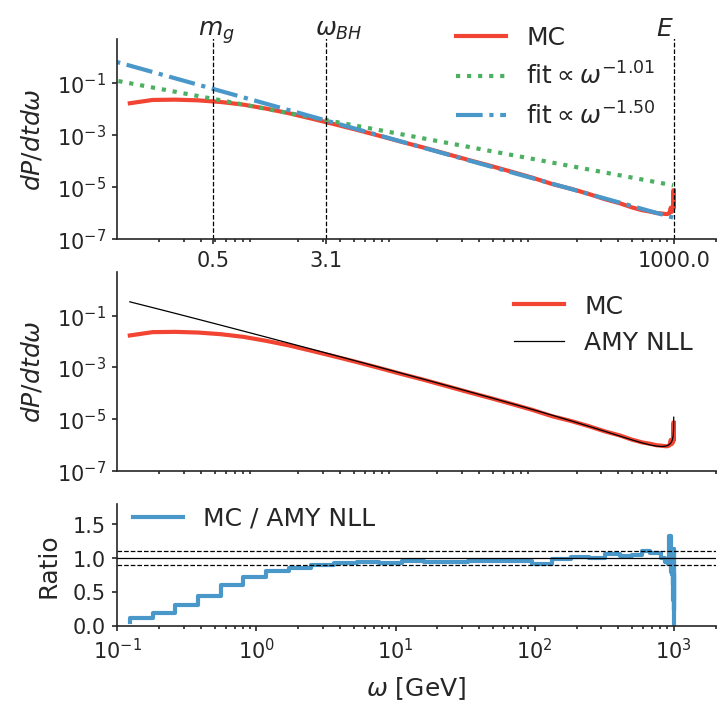
\includegraphics[width=.8\columnwidth]{spectrum.png}
}
\caption{The $q\rightarrow q+g$ splitting rate simulated in an infinite box with $T=0.5$ GeV. The quark energy is $E=1$ TeV. $\alpha_s = 0.1$. In the top plot, the spectrum $dR/d\omega$ (red line) is fitted to a power function $\omega^\lambda$ in different gluon energy regions. The green dashed line is fitted in the Bethe-Heitler region $\omega < \omega_{BH}\approx 2\pi T$; the blue dash-dotted line is fitted in the LPM region $\omega > \omega_{BH}$. The middle plot compares to the simulation to NLL solution to the AMY equation, and their ratio is shown in the bottom plot}
\label{fig:spectrum}
\end{figure}

In practice, to define a Monte-Carlo transport simulation an infinite medium limit and an eikonal limit of parton propagation, an ensemble of parton of certain species are initialized at a fixed energy $E_0$ and will be let propagate in the same direction.
Each time when a parton scatters elastically or splits, its splitting kinematics are taken down $\omega, k_\perp, t_0, \tau_f$, then the mother parton's energy is reset back to its initial value (a test in the eiknoal limit).
For elastic re-scatterings in the implementation of the LPM effect, the parton's energy is re-scaled back to the value before scatterings without changing its direction.
The system is evolved for a sufficiently long time $t_{\max}$, and only branchings that takes place within $[t_{\min}, t_{\max}]$ are analyzed to focus on the infinite time behavior of the simulation.

We start from the $q\rightarrow q+g$ channel.
The differential rate $dR/d\omega$ for a 1 TeV quark propagate through a medium of $T=0.5 GeV$ with coupling constant $\alpha_s = 0.1$ is shown in 
figure \ref{fig:spectrum}.
The vertical axis is the differential branching rate $dR/d\omega$, and the horizontal axis is the energy of the final state gluon $\omega$.
To better understand our result, we have put three ``landmark'' energy scales in the upper plot, which are the initial parton energy $E$, an estimate of the Bethe-Heitler energy $\omega_{\textrm{BH}}\sim\hat{q}_g \lambda_g^2 \sim 2\pi T$, and the screening mass $m_g = m_D/\sqrt{2}$.
In the LPM regime $\omega_{\textrm{BH}} < \omega$, the spectrum falls off as a power law with fitted exponent $-1.50$ (the blue dash-dotted line), and the in the Bethe-Heitler regime above the screening mass $m_g < \omega < \omega_{\textrm{BH}}$, the fitted power law exponent is close to $-1$ (the green dotted line).
These exponents are in good agreement with the theoretically expectation that $dR_{\textrm{BH}}/d\omega \propto \omega^{-1}$ and $dR_{\textrm{LPM}}/d\omega \propto \omega^{-3/2}$ from equations \ref{eq:incoh-dR} and \ref{eq:AMY-LL}.
The screening mass regulates the soft divergence of the spectrum below $m_g$.
One may notice a tiny increase of the spectrum when $\omega \rightarrow E$, this is region where the gluon takes a larger fraction of the initial quark's energy.

In the middle plot, we compare this result from simulation directly to the NLL solution of the AMY equation. 
As a remark, we have tuned the prefactor in the $b$-parameter to be $0.75$  by comparing to this theory prediction at $\alpha_s=0.1, E=1 \textrm{TeV}, T = 0.5 \textrm{GeV}$ for the $q\rightarrow q+g$ channel.
For the rest of the comparison with different coupling, parton energy, temperature, and channels, this parameter will {\bf not} be further tuned.
The simulation agrees with the NLL solution very well when $\omega \gg \omega_{\textrm{BH}}$ where the formula is valid.
The bottom plot show the ratio between the simulation and the theory, an level of $\pm 10\%$ agreement in the deep-LPM region is achieved in the static case.

\begin{figure}
\centering{
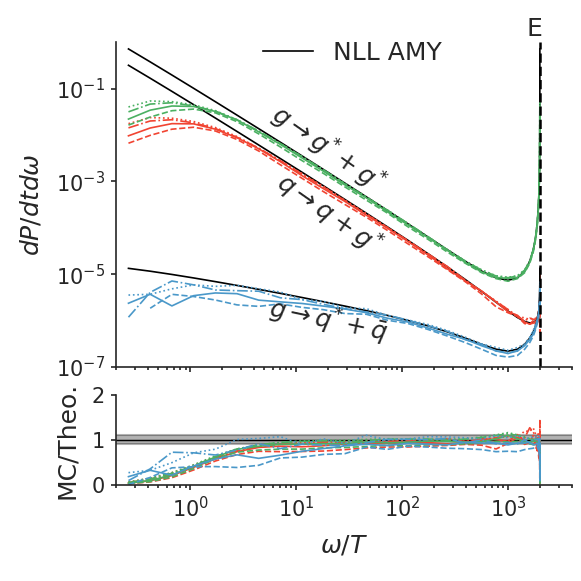
\includegraphics[width=.8\columnwidth]{channel_rate.png}
}
\caption{The rate of different channels $q\rightarrow q+g^*$, $g\rightarrow g+g^*$, and $g\rightarrow q^* + \bar{q}$ are plotted as functions of the daughter (labeled by "${}^*$") parton energy. The mother parton has a energy $E=1$ TeV. The medium temperature is $T=0.5$ GeV. $\alpha_s = 0.1$. The simulations (thick dashed lines) are compared to the NLL solutions (thin solid lines).}
\label{fig:channel_rate}
\end{figure}

Next, we would like to compare the simulation all the three channels in figure \ref{fig:channel_rate}.
The setup is the same as the figure \ref{fig:spectrum}.
The red, green and blue lines correspond to the differential branching rate of processes $q\rightarrow q+g^*$, $g\rightarrow g^*+g^*$ and $g\rightarrow q^*+\bar{q}$; the thin back lines are the NLL solution to the AMY equation.
The ``${}^*$'' sign denotes the final state parton whose energy is $\omega$.
For the case two final state gluons, both are taken into account in the simulation as they are identical particles.
We have discussed the feature the $q\rightarrow q+g$ in the previous paragraph. 
The spectrum shape of $g\rightarrow g+g$ process is very similar to the quark splitting channel in the range $\omega \ll E$, with a higher value.
The rate is symmetric with respect to $\omega = E/2$ due to its symmetric final states (though it is hard to tell from this double-log plot), so at large $\omega$, the rate goes up again.
The spectrum of $g\rightarrow q+\bar{q}$ is also symmetric with respect to $\omega = E/2$.
Though its final state consists of two different particle, the splitting function is still symmetric in this case.
We see that the simulation achieves a good agreement with the NLL solution in the deep-LPM region $\omega/T > 10$.

Next, we would like validate the simulation with different coupling constant and parton energies.
We choose both a relative small coupling $\alpha_s = 0.1 (g \approx 1.1)$ and a value closer to the phenomenology coupling $\alpha_s = 0.3 (g \approx 1.9)$, and vary the energy from $10$, $10^2$, to $10^3$ GeV.
The ratios between the simulation and the NLL solutions are shown in figure \ref{fig:sys-q2qg}, \ref{sys-g2gg} and \ref{fig:sys-g2qqbar}.
From these systematic comparison.
One see that the simulation reproduces the correct scaling in the LPM region, although due to the decreasing of the parton energy, this region also shrinks.
The overall performance of the modified Boltzmann transport in describing the inelastic processes in a large medium is good and under control.
One remaining problem is that the systematic deviation for the $g\rightarrow q+\bar{q}$ channel is bigger than the other two channels, as we did not include the backward region in its $2\rightarrow 3$ matrix-elements.

\begin{figure}
\centering
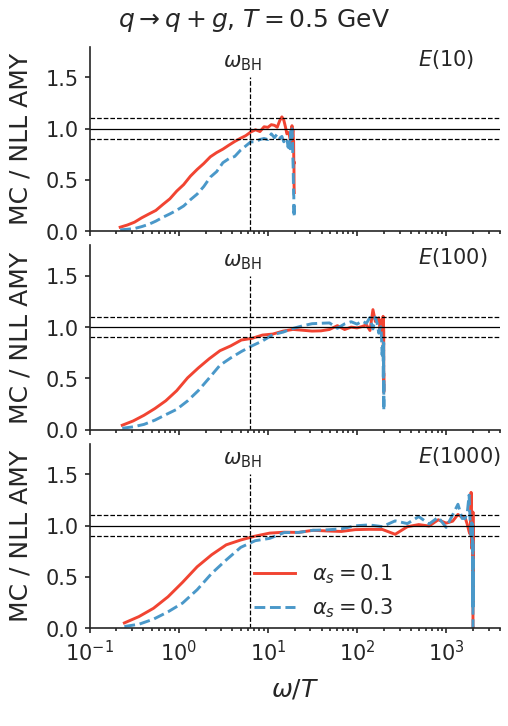
\includegraphics[width=.8\columnwidth]{spectrum_E_q2qg.png}
\caption{Ratios of splitting rate $dR/\omega$ between the modified Boltzmann simulation and the NLL solution for $q\rightarrow q+g$ splitting. The quark energies are $E$ is 10, 100, and 100 GeV from top to the bottom plot. 
And two coupling constants are used: $\alpha_s = 0.1$ (red solid lines) and $\alpha_s = 0.3$ (blue dashed lines).
$\omega$ stands for the gluon energy.
The horizontal dashed lines denote $\pm 10\%$ deviation from unity. }
\label{fig:sys-q2qg}
\end{figure}

\begin{figure}
\centering
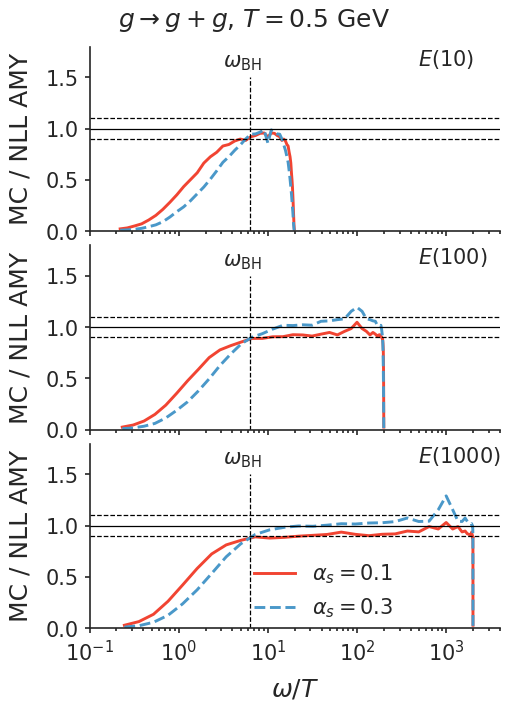
\includegraphics[width=.8\columnwidth]{spectrum_E_g2gg.png}
\caption{The same as figure \ref{fig:sys-q2qg}, but $g \rightarrow g + g$.}
\label{fig:sys-g2gg}
\end{figure}

\begin{figure}
\centering
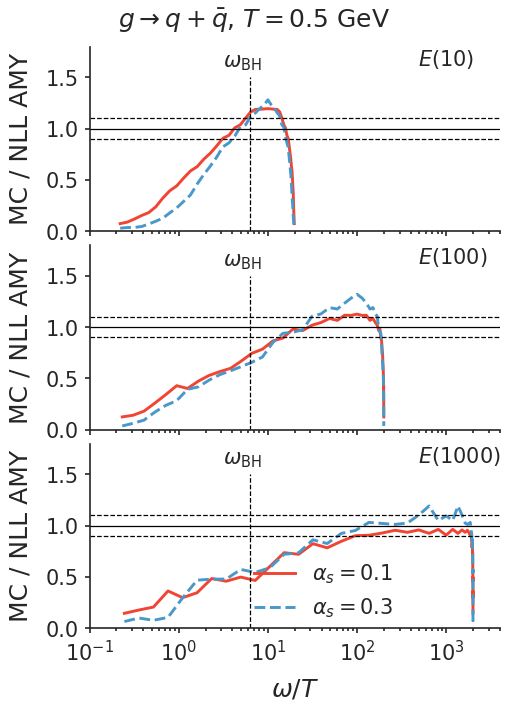
\includegraphics[width=.8\columnwidth]{spectrum_E_g2qqbar.png}
\caption{The same as figure \ref{fig:sys-q2qg}, but $g \rightarrow q + \bar{q}$.}
\label{fig:sys-g2qqbar}
\end{figure}

Finally, we validate the running coupling calculation in Fig. \ref{fig:running} using the $g\rightarrow g+g$ channel.
The theory curves (black lines) are obtained combining Eq. \ref{eq:AMY-LL} and Eq. \ref{eq:q3running}.
Different line styles correspond to the variation of the $Q_0$ value around an initial guess $m_D (E/T \ln(E/T) )^{1/4}$ by a factor of $2$ above and below.
For this 1 TeV parton, the scale $Q_0$ is actually very large and the running of $\alpha_s$ is rather slow, which explains the theory curve is not very sensitive to a factor of $4$ change in $Q_0$.
The simulation was performed using the running coupling prescription described in Section \ref{section:running}.
The overall shape of the spectrum in the deep LPM region is again well described by the modified Boltzmann simulation. 

\begin{figure}
\centering
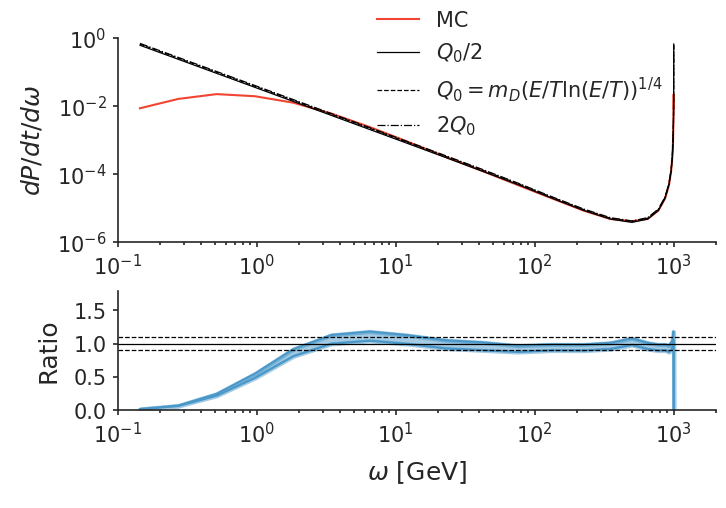
\includegraphics[width=.8\columnwidth]{running.png}
\caption{Comparing the simulation with running coupling constant the NLL solution with running $\alpha_s$ prescription.
The scale $Q$ in the emission vertex and in the theoretical formula for the effective transport parameter $\hat{q}_3$ (equation \ref{eq:q3running}) is chosen to be $1/2$, $1$ and $2$ times of the scale $\sqrt{\langle k_\perp^2\rangle}$ in equation \ref{eq:runscale}.
The ratio is shown in the bottom plot.}
\label{fig:running}
\end{figure}

\subsection{Branching in a finite / expanding medium}
We have made clear before that this approach is designed for interpolating the Bethe-Heitler region and the deep-LPM region in a large medium, and from the validation in the previous section, it indeed works very well.
However, the medium created in heavy-ion collisions were never in the large and static limit, its finite time and spatial extend, local hot spots fluctuations and the fast radial expansion can all make significant impact on the hard parton propagation. 
Therefore, we need to investigate how our approach would behave in a few more complex scenarios: a finite medium and and expanding medium, before applying such a model to phenomenological usage.

\paragraph{A semi-infinite medium}
Consider the semi-infinite medium with the static temperature profile,
\begin{eqnarray}
T = \begin{cases}
0 , z<0\\
T_0, z>0
\end{cases}
\end{eqnarray}
and hard partons are created at $z=0$ and propagate into the medium.
Deep inside the medium, the medium induced radiation should be getting asymptotically close to the calculation in an infinite medium.
At the boundary, there is a complicated interference between medium scatterings centers and the hard production vertex.
For a thin medium where the path length is short compared to the formation time, these interference terms can be worked out in the ``opacity expansion", or by analyzing the propagator in the path-integral formalism with the semi-infinite temperature profile.
This boundary effect results in a path length dependence of the medium induced branching rate that starts from zero at $t=0$ and gradually approach the asymptotic value in a large medium.
The resulting parton energy loss rate is significantly reduced due to this effect, and scales quadratic with the path length $\Delta E \propto L^2$ near the boundary and at larger times, it transits to $\Delta E \propto L$.

It is true that our approach is designed for a large medium, but it also displays certain finite size effect. 
Remember that the branchings in the modified transport approach takes a finite amount of time, and those branching that becomes independent at time $t$ are actually initiated by a $2\rightarrow 3$ processes at from a wide range of scattering centers in the past $t' = t - \tau_f$.
Therefore, if the medium is semi-infinite, and there were no scattering centers before $t' = t-\tau_f < 0$, then the medium-induced contribution to the branchings at time $t$ will be reduced.
This reduction gets weaker and weaker when the condition $t-\tau_f > 0$ can be satisfied by more and more induced branchings and eventually, when $t\gg \langle \tau_f\rangle$, this boundary effect dies off in the simulation. 
Of course, it is can not reach an quantitative level of agreement with the theory at $L \lesssim \tau_f$ since the interference pattern is not implemented.
We would like to check if this simulation boundary effect qualitatively mimic the interference physics that happens near the boundary.

\begin{figure}
\centering
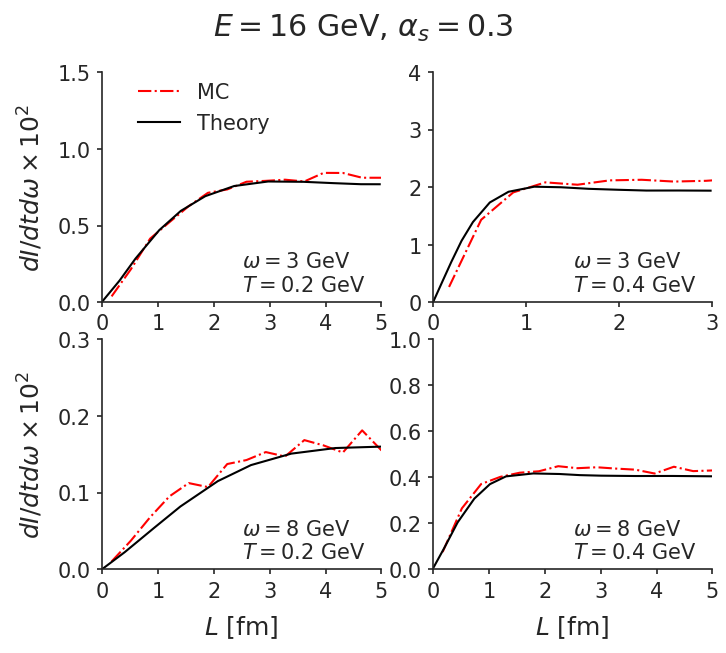
\includegraphics[width=.8\columnwidth]{spectrum_L.png}
\caption{The path-length dependence of the simulated $q\rightarrow q+g$ emission rate $dR/d\omega$ comapred to the direction calculation of formula \ref{eq:full-theory} from \cite{CaronHuot:2010bp}. $\alpha_s = 0.3$. The quark energy is $16$ GeV. The left and right columns have medium temperature $T=0.2$ and $0.4$ GeV respectively. The top and bottom rows show the differential rate at $\omega = 3$ and $8$ GeV.}
\label{fig:spectra-L-alphas=0.3}
\end{figure}

In Figure \ref{fig:spectra-L-alphas=0.3}, the differential rate obtained from simulation is compared to the numerical solution of the full leading order calculation for a finite medium.
The horizontal axis is the time of travel by the hard parton (path length divided by the speed of light), and each subplot shows how the branching rate changes as a function of time with different medium temperatures ($T=0.2$ GeV on the left, $T=0.5$ GeV on the right) and at different branching parton energy ($\omega=3$ GeV at the top, $\omega=8$ GeV at the bottom).
The theory curves are taken from the references \cite{CaronHuot:2010bp} for a 16 GeV parton with coupling constant $\alpha_s = 0.3$, and the red lines are our simulation.
The theory curve first increases linearly and then turn over to a constant value in the large medium limit for $t \gg \sqrt{2x(1-x)E/\hat{q}_3}$.
The simulation, as expected, reproduces the large time limit of the rate.
Moreover, we find that the current implementation also predicts the qualitative ``turn over'' of the spectra at finite path length.
The original paper only publish this calculation for a $16$ GeV quark. 
To validate if this qualitative agreement also holds at higher parton energies, we implement the numerical approach \cite{CaronHuot:2010bp} and compute the theoretical curves for $E=100$ GeV partons.
The comparison of simulation and numerical solutions are shown in figure \ref{fig:spectra-L-alphas=0.3-E100} and again, we found a qualitative agreement with the theoretical finite size effect.

\begin{figure}
\centering
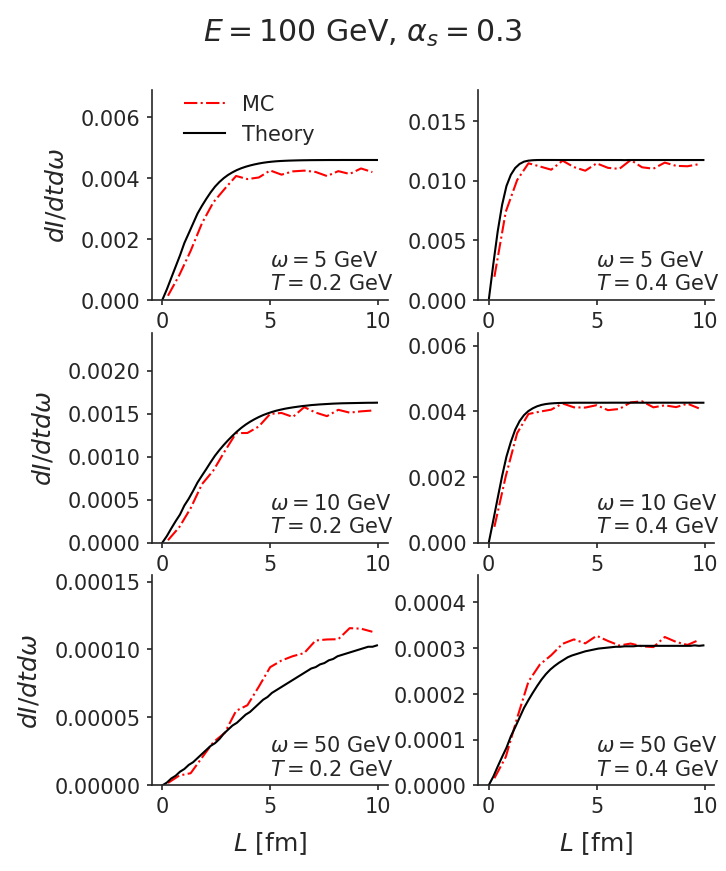
\includegraphics[width=.8\columnwidth]{spectrum_L_100.png}
\caption{The same as figure \ref{fig:spectra-L-alphas=0.3-E100}, but the initial quark energy is $100$ GeV, and is plotted for gluon at 5 (top), 10 (middle) and 50 (bottom) GeV.}
\label{fig:spectra-L-alphas=0.3-E100}
\end{figure}

\paragraph{An expanding medium}
Fast radial expansion is another important feature of the medium in heavy-ion collisions.
It causes the temperature to decrease drastically in the early stages of the expansion and introduces another time scale in which the medium temperature changes notably.
Assume a simplified power-law changing temperature profile
\begin{eqnarray}
T(\tau; \nu)^3 = T_0^3\left(\frac{\tau_0}{\tau}\right)^{2-1/\nu}.
\end{eqnarray}
The $\nu$ parameter controls the rate of expansion. 
$\nu = 1/2$ is the static medium limit, and $\nu=1$ is the Bjorken flow.
We can define the following medium expansion time, over which the transport parameter changes significantly,
\begin{eqnarray}
\tau_{\textrm{ex}} = \left(\frac{d\ln(T^3)}{d \tau} \right)^{-1} = \frac{\tau}{2-1/\nu}.
\end{eqnarray}
The larger the $\nu$ parameter is, the smaller the expansion time scale.
With $\tau_0 \sim 1$ fm/$c$, the expanding time scale can be short enough that energetic branchings already probes the changing temperature profiles within its formation time $\tau_f > \tau_{\textrm{ex}}$.
One consequences of this fast changing of temperature is that, for these branchings $\tau_f > \tau_{\textrm{ex}}$, the transition probability over a finite amount of time can not be well approximated by integrating rates that are calculated in an infinite box defined by the local temperatures,
\begin{eqnarray}
\frac{dP(t_1, t_2)}{d\omega} \neq \int_{t_1}^{t_2} \frac{dR_{\infty}(T(t))}{d\omega} dt,
\end{eqnarray}
where is the rate obtained by solving the branching rate in the infinite medium setup. 
This approach is employed in transport models like MARTINI and TEQULIA \cite{Jeon:2003gi,Schenke:2009gb,Dai:2019hbi}.
Our approach akes into account the changing of the medium temperature (and also flow velocity).
This is because the rescattering procedure that determines amount of suppression is performed along the trajectory of the hard partons and therefore naturally includes the effect of the cooling of the medium.
The typical formation time determined by the rescattering procedure is also changed by the expansion.
Recall that in a static medium the dimensionless combination that enters the leading-log formula is the $t/\tau_f \sim t \sqrt{\omega/\hat{q}}$, but with a $\hat{q}$ that is decreasing with temperature.
The self-consistent determination of the formation time requires the following relation to hold on average,
\begin{eqnarray}
t_2 - t_1 &=& \frac{2x(1-x)E}{k_{\perp}^2(t_1) + \int_{t_0}^{t} \hat{q}(\tau) d\tau},\\
\hat{q}(\tau) &=& \hat{q}(\tau_0) \left(\frac{\tau_0}{\tau}\right)^{2-1/\nu}
\end{eqnarray}
Neglecting the initial transverse momentum at $t=t_1$, we have the characteristic time scale $\Delta t = t_2 - t_1$ of this procedure in the expanding medium temperature profile as
\begin{eqnarray}
1 = \sqrt{\frac{\hat{q}(t_0)}{2x(1-x)E}} \tau_0 \sqrt{\frac{\nu-1}{\nu}} \left(\frac{\Delta t}{\tau_0}\right)^{1/2\nu}
\end{eqnarray}

\begin{figure}
\centering
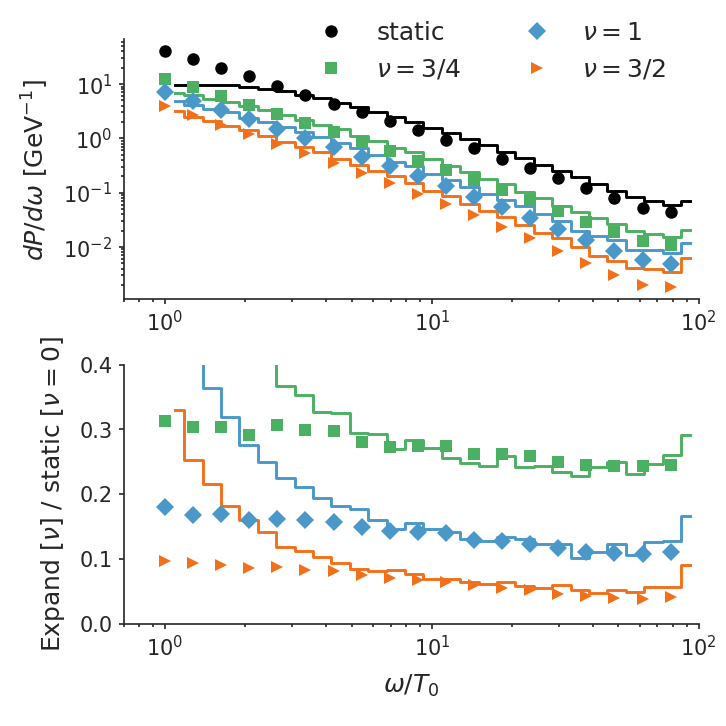
\includegraphics[width=.8\columnwidth]{spectrum_Bjorken.png}
\caption{Top plot: the simulated spectrum (diffusion plues diffusion-induced radiation only) using the parametric medium with expansion parameters $\nu = 0$ (static, black), $3/4$ (green), $1$ (Bjorken, blue), and $3/2$ (orange). The analytic results are shown in symbols and simulations in lines. $\alpha_s=0.3$. The expansion starts at $\tau_0 = 0.2$ fm/$c$ with an initial temperature $T_0 = 1$ GeV. Bottom plot: the ratios between calculation (simulation) in an expanding medium to that in the static medium.}
\label{fig:Bjorken-BDMPS}
\end{figure}

Making comparison to theoretical calculations, we make use of a result obtained in the BDMPS framework \cite{Baier:1996kr,Baier:1998yf}.
Using the power-law decreasing temperature profile, the obtained branching probability for the $q\rightarrow q+g$ splitting is \cite{Baier:1998yf},
\begin{eqnarray}
\frac{dP}{d\omega} &=& \frac{\alpha_s}{2\pi E}P_{q\rightarrow qg}(x)\mathfrak{Re}\int_{\tau_0}^{\tau_0+L}\frac{dt_f}{t_f}\int_{\tau_0}^{t_f}\frac{dt_i}{t_i} \frac{1}{\nu^2}\\
\nonumber
&& \left.\left[ I_{\nu-1}(z_i)K_{\nu-1}(z_f)-I_{\nu-1}(z_f)K_{\nu-1}(z_i)\right]^{-2}\right|_{\omega=xE}^{\omega=\infty},\\
z_{i,f} &=& 2i\nu \sqrt{\frac{\hat{q}_g(1-x+C_F/C_A x^2)}{2(1-x)\omega}} \tau_0 \left( \frac{t_{i,f}}{\tau_0}\right) ^{1/2\nu}.
\end{eqnarray}
This result goes back to the static BDMPS result \cite{Baier:1996kr} when $\nu=1/2$.
One potential problem of comparing the formula to our simulation is that this BDMPS calculation works in the multiple-soft limit (leading log).
Therefore, we used only the diffusion-induced radiation in the simulation and turned off the large-$Q$ $2\rightarrow 3$ scattering part.
Also as mentioned before, in the absence of the pertrubative tail in the collision kernel, $b=0.75$ is used without the logarithmic correcting factor in equation \ref{eq:NLL-b}.
In addition, we will not try to make a direct comparison of the spectra (top of figure \ref{fig:Bjorken-BDMPS}), but focusing more on the ratio between the expanding calculation/simulation over the static calculation/simulation instead (bottom of figure \ref{fig:Bjorken-BDMPS}).
This ratio reflects the change of the shape of the spectra due to the dropping of temperature.

The simulation uses a medium with initial temperature $T_0=1$ GeV at $\tau_0=0.2$ fm/$c$ and lasts until $\tau = 20$ fm/$c$ using four different expansion rate $\nu = 1/2, 3/4, 1, 3/2$.
These choice of numbers corresponds to a static medium, a slowly expanding medium, the Bjorken flow, and a faster-than-Bjorken expansion.
We found that when $\omega \gg T_0$, the degree of change in the radiation spectra is well reproduced by the modified transport simulations.

\begin{figure}
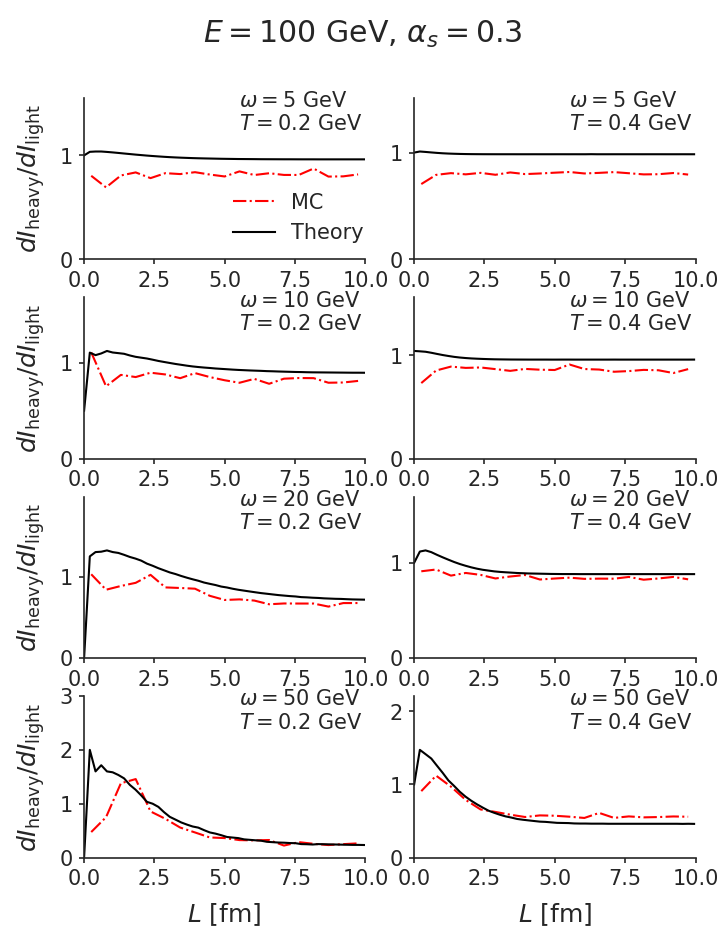
\includegraphics[width=\columnwidth]{mass.png}
\caption{The mass dependence of the radiation spectrum $q\rightarrow q+g$, presented as the ratio of bottom $dR/d\omega$ over the light quark $dR/d\omega$, as functions of path length. The left and right columns use temperatures 0.2 and 0.4 GeV. Different rows (from top to bottom) plot cases for gluon energy $\omega = 5, 10, 20, 50$ (GeV).}
\label{fig:mass}
\end{figure}

\subsection{Heavy quark and thermalization test}
Finally, we check the model performance for heavy quarks.
For short, to implement mass effect to the modified transport approach for inelastic scatterings, we use massive kinematics for the heavy quarks, include the mass term in the formation time, and implement the dead cone approximation after the transverse momentum is broadened by elastic collision.
The theory curves are obtained by solving the exact equation with a effective mass term,
\begin{eqnarray}
m_{\textrm{eff}}^2 = (1-x)m_g^2 + x^2 M^2
\end{eqnarray}
which includes both the thermal mass of the gluon and the current mass of the heavy quark.
We present the comparison between the simulation and the theory in terms of the ratio between the differential branching rate of the heavy quark (charm mass at 1.3 GeV, bottom mass at 4.2 GeV) and the light quark.
In figure \ref{fig:mass} for the bottom quark case, the horizontal axis is the path-length, and the vertical axis is the ratio.
Different rows take different radiated gluon energies, and different  columns has medium temperatures at $0.2$ GeV (left) and at $0.4$ GeV (right) respectively.
The initial bottom quark energy is 100 GeV and the coupling is $\alpha_s=0.3$.
We see that the dead-cone approximation better agrees with the theory calculation at larger $x$ and larger path-length.
Deviations observed at small path length is understand as the limitation of our implementation to the large medium, and should be better treated by the opacity expansion. 
The deviation at small $x$ is interesting, particularly, the theory almost predicts an identical heavy quark radiation spectra as the light quark. This absent of dead cone at small-$x$ is already observed in early works of heavy quark energy loss study in both the GLV framework and the BDMPS framework.
This means that the treatment of the mass effect is not as simple as the dead-cone approximation and should be improved in the future.


\paragraph{Thermalization of heavy quark}
\begin{figure}
\centering
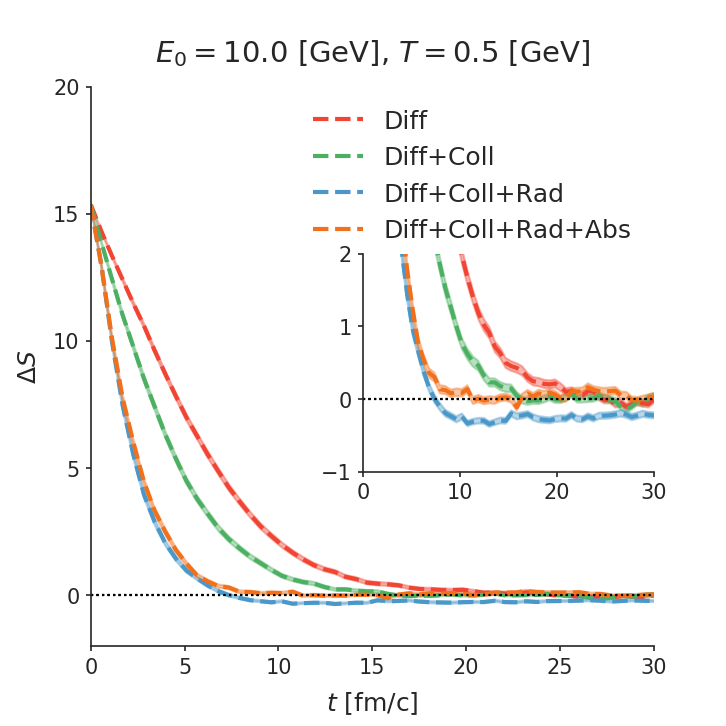
\includegraphics[width=.8\textwidth]{thermalization.png}
\caption{Approaching to thermal equilibrium of heavy flavor is quantified as the change of $\Delta S$ (defined in equation \ref{eq:DeltaS}) as function of time.. The red dotted lines includes elastic processes only. The green dashed line further includes $2\rightarrow 3$ and $1\rightarrow 2$ processes. The blue solid lines turn on the detailed balance processes $3\rightarrow 2$ and $2\rightarrow 1$.}
\label{fig:thermalization}
\end{figure}
Heavy quark's large mass made it takes longer time to thermalize and the low-$p_T$ end of the heavy quark production in the heavy-ion collision can carry the information non-equilibrium dynamics.
To extract the degrees of thermalization, one has to make sure the correct thermalized limited is achieved in the transport model, given enough time of evolution.
This is trivial for large-angle elastic scatterings and diffusion processes as long as the correct Einstein relation is imposed.
The $n\rightarrow n+1$ body radiative process is approximated by a initial $2\rightarrow 3$ or $1\rightarrow 2$ process and a sequence of elastic interactions; therefore, in principle the $n+1\rightarrow n$ absription processes need to be treated on the same footing to restore the detailed-balance in the modified-Boltzmann equation.
This can be done but is over complicated.
Here we argue that close to a few times of temperature, the LPM effect is not that strong that an incoherent implementation of the absorption is enough to study the bulk of particles close to thermal distribution.

We define a quantity $\Delta S$ to measure the approaching of thermal distribution $f_0 = e^{-E/T}$ of an ensemble of heavy quarks,
\begin{eqnarray}
\Delta S = - \langle \ln f_0 \rangle - S_0 \\
 &=& - \frac{1}{N}\sum_i\ln f_0(E_i) - \frac{\int dp^3 f_0 ln(f_0)}{\int dp^3 f_0}
 \label{eq:DeltaS}
\end{eqnarray}
Where the first term the the ensemble average of the the function $-\ln f_0$, and the subtracted term is proportional to the entropy of distribution $f_0$.
Note that the quantity is zero if the ensemble thermalize.
If the system is approaching thermal distribution with an effective temperature such that $f = e^{-E/T'}$, then $\Delta S$ is 
\begin{eqnarray}
\Delta S = \frac{\int dp^3 E/T e^{-E/T'}}{\int dp^3 e^{-E/T'}} - S_0 = \frac{T'-T}{T}
\end{eqnarray}
which is a measure of the deviation of the effective temperature from the thermal bath temperature.

Using this definition, we plotted $\Delta S$ as a function of time for 1000 heavy quark that are initialized at 10 GeV.
The temperature of the thermal bath is 0.5 GeV and we used a fixed $\alpha_s = 0.3$.
Under the influences of diffusion (red) and diffusion plus large-angle elastic collisions (green), $\Delta S$ decreases from a large value until fluctuating around zero after 25 fm/$c$ (red) and $15$ fm/$c$ (green).
Now, adding the radiative processes (blue), the $\Delta S$ reaches a value below zero, which is the false equilibrium.
Only after the balancing processes of parton absorption are also included (orange), the correct thermal equilibrium limit is restored. 
We also found that the absorption process only sets in when the ensemble is close enough to the thermal distribution, as the bue line and the orange line are almost overlapped until $\Delta S$ dropped to 0.3.
This is because the absorbed gluon follows the thermal distribution in the medium while phase-space for a high energy parton $E\gg T$ to absorb a low energy gluon is very limited $x<T/E$, compared to radiation processes where the value of $x$ is not restricted by the Boltzmann factor $e^{-xE/T}$.

\section{Comments on two other inelastic process implementations}
I find it beneficial to discuss two other inelastic processes implementations for reader's references. 
They are termed as the ``coherence factor" approach and the ``blocking radiation" approach.
I had used the previous approach in my earlier studies \cite{Ke:2018tsh}, but it is the problems I encountered in this method that later motivates the development of the ``modified Boltzmann transport'' method. 
I shall show in this section that in the deep-LPM region, the ``coherence factor" approach still qualitatively agrees with the power counting of the LPM suppression $\lambda_{el}/\tau_f$, though it only includes the effect of one medium scattering centers and the method can be logarithmic dependent on the infrared cut-off.
The ``blocking radiation'' approach, however,  does not reproduce the power counting of of the LPM suppression.
These two approach, together with the ``modified Boltzmann'' approach will be compared later using the ``energy loss" of a fixed energy quark.
First, we introduces these two other approaches.

\subsection{The coherence factor approach}
This approach is first implemented in the improved Langevin equation \cite{Cao:2013ita}, using the single medium-induced radiation probability from the higher-twist calculation \cite{Majumder:2009ge,Wang:2001ifa} and a prescription for multiple emissions.
The higher-twist formula of medium-induced radiation is derived for a high virtual parton, including the interference of the hard production vertex and one medium scattering center.
The single radiation rate reads,
\begin{eqnarray}
\frac{dN_g}{dx dk_\perp^2 dt} = \frac{\alpha_s P(x)\hat{q}_g}{\pi k_\perp^4} 2\left(1-\cos\frac{t-t_0}{\tau_f}\right), \tau_f = \frac{2x(1-x)E}{k_\perp^2}
\end{eqnarray}
Here the radiation rate is a time-dependent ($t$) one due to the interference with the hard production at time $t_i$. 
Note that the interference factor cancels the collinear divergence. 
The only divergence comes from soft emission $x\rightarrow 0$. 
This divergence is not a problem for computing more physical quantities such as the energy loss, as it will be balanced by the gluon absorption processes.
However, in order to apply rate formulation, an infrared cut-off $x>x_c$ has to be introduced. 

The advantage is that if there is only one radiation, then sampling the time dependent rate indeed reproduces the High-Twist calculation.
However, the ambiguity rises from the way it handles multiple emissions.
For example, one can compute the average number of emission by integrating this formula along the trajectory of the hard parton through and then samples the fluctuating number of emission with a Poisson distribution.
But of course, this would assume the parton energy is not significantly changed during the process, and it is not clear how the presence of more than one scattering center would change this picture.
Here we would like to discuss another method in dealing with multiple emission using the high twist formula in a time evolution manner \cite{Cao:2013ita}.
The algorithm goes as follows:
\begin{itemize}
\item[1.] Choose an infrared cut-off for the gluon energy $x_c \propto T/E$, and a small enough time step $\Delta t$, so that the average number of emission is much smaller than $1$ to suppress multiple emission within $\Delta t$,
\begin{eqnarray}
\langle N_g \rangle = \Delta t \int_{x_c}^1 dx \int dk_\perp^2 \frac{dN_g(t-t_0)}{dx dk_\perp^2 dt} \ll 1.
\end{eqnarray}
\item[2.] Sample N according to a Poisson distribution with $\langle N_g \rangle$. For $\langle N_g \rangle \ll 1$, it is sufficient to sample the two leading cases of $N=0, 1$, as the probability to have more than 1 emission is negligible ($P_{N>2} = 1-e^{-\langle N_g \rangle}-e^{-\langle N_g \rangle}/\langle N_g \rangle = O(\langle N_g \rangle^2) \ll P_1 \ll P_0$).
\item[3.] If $N=0$ then propagate the parton to the $t+\Delta t$. If $N=1$, then sample the emission gluon's $x$, and $\vec{k_\perp}$ by the differential rate. {\it Meanwhile, $t_0$ is set to $t$}, so that the next emission's probability will accumulated from zero again.
\item[4.] Proceed for the next time step.
\end{itemize}
We found that the key step here is resetting the clock $t_0 = t$ for the parton after every emission.
As a result, from the second emission, the time difference that appears in the interference factor $t-t_0$ are the one measuring between two medium scattering centers.
Therefore, we will not interpret this procedure as the high-twist rate (interference between initial hard vertex and one medium collision center) starting from the second emission;
instead we understand it as an ansatz, from the second emission, to treat medium-induced emission in a large medium, as it do not require any information to the production vertex.

Considering it only includes one medium scattering center in the trigger the radiation, one wonders if this approach reproduces any in-medium radiation features predicted by the theory.
It is not immediately clear that what this iterative procedure predicts  expect through simulations. 
But if one pondering on the meaning of the ``clock resetting" step, then the typical $\Delta = t-t_0$ between two emissions are a time scale within which the emission probability reaches order one,
\begin{eqnarray}
1 \sim \int_{t_0}^{t} dt\int_{x_c}^1 dx \int dk_\perp^2 \frac{dN_g(t-t_0)}{dx dk_\perp^2 dt}.
\end{eqnarray}
With this key observation, after a few step of algebra, we are able to learn the qualitative feature of this approach.
Taking the soft approximation $P(x) \sim 2/x$, $\tau_f\sim 2xE/k_\perp^2$, and perform the time integral first, then the $k_\perp$ integral with limits from $0$ to $xE$.
\begin{eqnarray}
1 &\sim& 4\alpha_s\hat{q}\Delta t \int_{x_c}^1 \frac{dx}{x} \int \frac{dk_\perp^2}{k_\perp^4}\left(1-\frac{\sin(\Delta t/\tau_f)}{\Delta t/\tau_f}\right)\\
&=& \alpha_s\hat{q}_g \Delta t^3 \int_{\frac{\Delta t E x_c}{2}}^{\frac{\Delta t E}{2}} 
\frac{du}{u^2} \frac{u^2 \mathrm{Si}(u) -2u + \sin(u) + u\cos(u)}{u^2}\\
&=& \frac{\alpha_s\hat{q}_g \Delta t^3}{3u^3} \left(
u^3\mathrm{Ci}(u)-3u^2\mathrm{Si}(u) \right.\\\nonumber
&&\left.\left.- u^2 \sin(u) +3u-\sin(u) - 2u\cos(u)\right)\right|_{\frac{\Delta t E x_c}{2}}^{\frac{\Delta t E}{2}} 
\end{eqnarray}
This final integral of $x$ (reparametrize by $u = xE\Delta t/2$) would have been logarithmic divergent if we had not cut it at $x_c$ at the lower bound.
The result has the following expansion at small $u$: $\frac{1}{18}(6\ln(u)+6\gamma_E - 17)$ and decay to $0$ at infinite therefore a good proxy is to use the small-$u$ expansion but cut-off the upper bound of $u$ at its zero, and finally
\begin{eqnarray}
1 &\sim&  \frac{\alpha_s\hat{q}\Delta t^3}{3}\ln\frac{2}{ x_c E \Delta t } \propto (g^2 T \Delta t)^3 \ln\frac{2}{ x_c E \Delta t }
\end{eqnarray}
Now, it is clear that this procedure of implementing multiple emission inside the medium resets the clock in the interference factor every $1/g^2T$ up to certain logarithm dependence on the infrared cut-off, which is the order of the elastic collision mean-free-path.
Put this estimated $\Delta t$ back into the interference factor $2(1-\cos(\Delta t/\tau_f))$, one indeed find that the radiation spectrum will be strongly suppressed if the formation time is much greater than $\Delta t\sim \lambda_{el}$.

This suppression certainly mimic some property of the in-medium LPM effect, but is introduced by a very different mechanism.
Remember that the LPM effect is the suppression of single particle emission rate through multiple collision with the medium, without any information about how subsequent emissions are correlated. 
While the interference factor approach mimic the effect of the LPM suppression through correlation between subsequent emissions.
This will introduce several problems: 
\begin{itemize}
\item[1.] The correlation between subsequent emissions is in fact physics beyond leading order and requires new type of diagrams to be computed.
\item[2.] As we have seen, this procedure is affected by the choice of the infrared cut-off. Though its dependence is very weak, it is still a dependence that we try to avoid.
\end{itemize}

\subsection{The ``blocking radiation'' approach}
This is another approach we found in the literature \cite{ColemanSmith:2012vr}.
I would like to show that this approach is more problematic than the previous one, because it suppresses radiation with $\tau_f > \lambda_{\textrm{inel}}^{\textrm{incoh}}$ but not $\tau_f > \lambda_{\textrm{el}}$.

In this approach, the splitting is also first generated through an incoherent processes at time $t_0$, and then the self-consistently determination the formation time by elastic broadening. 
But its LPM suppression is introduced by requiring no other radiation is allowed from this radiator within the time from $t_0$ to $t_0 + \tau_f$.
This clearly introduces a correlation between subsequent emission, while the LPM effect concerns only the one particle emission rate.
While in our approach, the suppression is implemented by accepting the process with probability $\sim \lambda_{el}/\tau_f$, and more importantly, other emissions are unaffected by the current ``imaginary splitting" as most of them would be rejected without causing any physical effect.

A closer investigation reveals bigger problem.
Moreover, this ``blocking radiation" approach effectively reduces every $\tau_f/\lambda_{inel}$ incoherent emission to one, resulting only an overall reduction in the radiation spectrum without changing its shape.
And the suppression factor $\lambda_{inel}/\tau_f$ is different from the expected one, this is in fact an order of $\alpha_s$ wrong as the mean-free-path of the incoherent radiation rate contains one more power of $\alpha_s$ than $\lambda_{el}$.

\begin{figure}
\centering
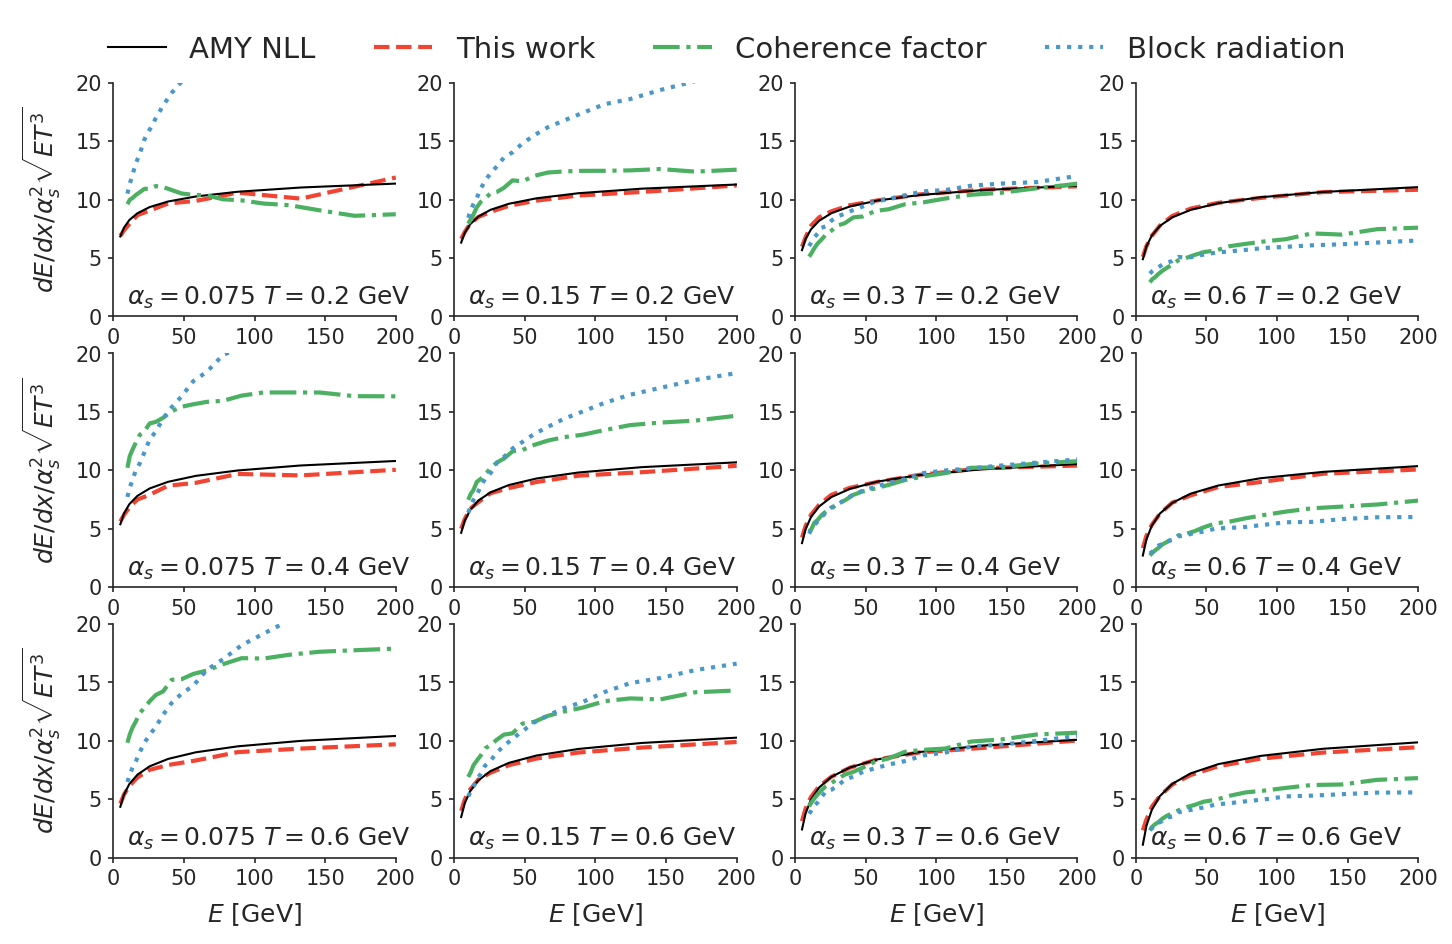
\includegraphics[width=1.\textwidth]{Eloss_infinite.png}
\caption{Energy loss per unit path lengh $dE/dx$ as a function of energy $E$, temperature $T$ and coupling constant $\alpha_s$. Each column corresponds to a value of the coupling constant $\alpha_s = 0.075, 0.15, 0.3$, and $0.6$ (from left to right). Each row corresponds to a temperature of $T = 0.2, 0.4$, and $0.6$ GeV (from top to bottom). $dE/dx$ is divided by the expected scaling $\alpha_s^2 \sqrt{ET^3}$. The MC implementations in this work (red dashed lines) is compared to the ``coherence factor" approach (green dash-dotted lines) and the ``block radiation" approach (blue dotted lines). The analytic results are denoted as black solid lines.}
\label{fig:eloss-inf}
\end{figure}

\begin{figure}
\centering
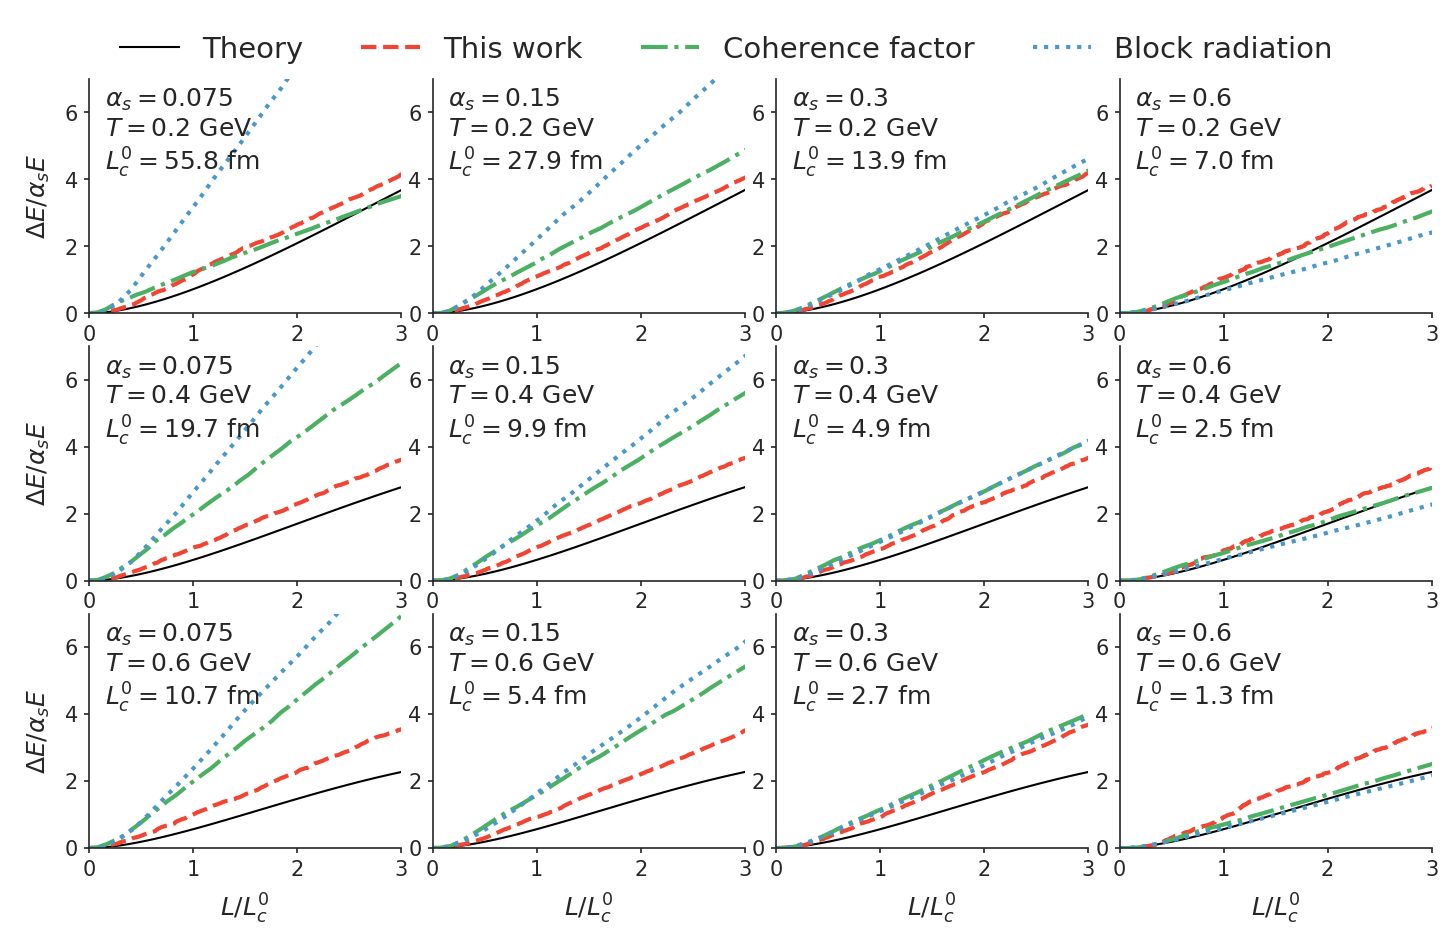
\includegraphics[width=1.\textwidth]{Eloss_Ldep.png}
\caption{Energy loss $\Delta E$ as a function of path length $L$, temperature $T$ and coupling constant $\alpha_s$. Each column corresponds to a coupling constant of value $\alpha_s = 0.075, 0.15, 0.3$, and $0.6$ (from left to right). Each row corresponds to a temperature of value $T = 0.2, 0.4$, and $0.6$ GeV (from top to bottom). $\Delta E$ is scaled by $\alpha_s E$ and $L$ is scaled by an estimated critical path length $L_c^0 = \sqrt{E/\hat{q}_0}$, $\hat{q}_0 = C_A \alpha_s T m_D^2$. The MC implementations in this work (red dashed lines) is compared to the ``coherence factor" approach (green dash-dotted lines) and the ``block radiation" approach (blue dotted lines). The analytic results for a thin medium are denoted as black solid lines.}
\label{fig:eloss-ldep}
\end{figure}

\subsection{Energy loss comparison among the three approaches}
In Figure \ref{fig:eloss-inf}, we show the calculation of energy loss per unit path length $dE/dx$ of a quark in an ``infinitely large" medium. 
Technically, $dE/dx$ is measured after an evolution time long enough ($L\gg L_c$) that finite size effects have faded away.
The results presented are normalized by $1/(\alpha_s^2 \sqrt{ET^3})$ in anticipation of the scaling $dE/dx \propto \alpha_s^2 \sqrt{ET^3}$.
For each column, we double the value of $\alpha_s$ and for each row, the temperature is increased by $0.2$ GeV. 
Within each subplot, the parton energy varies from $10$ GeV to $200$ GeV.
Different Monte Carlo implementations of the LPM effect are shown in colored lines, AMY NLL results are shown as black bands (we only integrate $\omega$ above the the Debye mass to calculate the AMY energy loss). 
Without a surprise, the ``modified approach" approach (red-dashed lines) reproduces the energy, temperature, and coupling constant dependence of AMY NLL energy loss very well.
The ``coherence factor" approach (blue-dash-dotted lines) has a similar energy and temperature dependence to that of the theoretical baseline; however, it systematically deviates from the baseline for different values of the coupling constant in a logarithmic manner.
For the ``block radiation" approaches, the deviations from the baseline regarding their $\alpha_s$-dependence are even bigger and the energy dependence also gets worse, which is not surprising as we have discussed its problem.

Next we examine the path-length ($L$) dependence of the energy loss $\Delta E$ of a quark with an initial energy of $E = 200$ GeV in a finite medium in Figure \ref{fig:eloss-ldep}.
Again, each column uses a different coupling constant and each row uses a different temperature. 
The path length within each subplot is varied up to four times $L_c^0$.
Here $L_c^0 = \sqrt{E/\hat{q}_0}$ with $\hat{q}_0 = C_A \alpha_s T m_D^2$ estimating the critical path length below which one expects a clear non-linear path-length dependence.
All three implementations show the non-linear increase of $\Delta E$ as function of $L$.
The ``modified Boltzmann" approach stays close to the theory calculations when $L<L_c^0$ for all cases, while the other two approaches deviate systematically as $\alpha_s$ is varied, similar to our previous findings for the energy-loss in the infinite matter case.

\section{Few-body matrix-elements}
\label{transport:ME}
This section provides the detailed $2\leftrightarrow 2$ and $2\leftrightarrow 3$ matrix-elements we used in the transport model.
The $2\leftrightarrow 2$ results are standard and we do not re-derive here.
The $2\leftrightarrow 3$ cross-sections are more complicated and a detailed derivation is attached to show the approximations we made for readers reference.

\subsection{$2\leftrightarrow 2$ processes}
The two-body scatterings between quarks, anti-quarks and gluons are standard and we quote the results from existing references \cite{RevModPhys.59.465}.
For a light parton scattering, we keep only $\hat{t}$-channel contribution, the $\hat{s}$ and $\hat{u}$ channel contribution are suppressed at high energy.
\begin{eqnarray}
\overline{|M_{q_1q_2\rightarrow q_1q_2}|^2} &=& \frac{64\pi^2 \alpha_s^2}{9} \frac{s^2+u^2}{t^2} \\
\overline{|M_{gg\rightarrow gg}|^2} &\approx& 72\pi^2 \alpha_s^2 \frac{-su}{t^2}
 \\
\overline{|M_{qg\rightarrow qg}|^2} &\approx& 16\pi^2 \alpha_s^2 \frac{s^2+u^2}{t^2}
\end{eqnarray}
For the heavy quark, since we are interested in its diffusion dynamics at low $p_T$, we uses the exact leading order matrix-element in the vacuum.
\begin{eqnarray}
\overline{|M_{Qq\rightarrow Qq}|^2} &=& \frac{64\pi^2\alpha_s^2}{9} \frac{(M^2-u)^2 + (s-M^2)^2 + 2 M^2 t}{t^2}
\nonumber
\\
\overline{|M_{Qq\rightarrow Qq}|^2} &=& \pi^2 \left\{
32\alpha_s^2 \frac{(s-M^2)(M^2-u)}{t^2} \right.
\nonumber
\\
&+&\frac{64}{9}\alpha_s^2 \frac{(s-M^2)(M^2-u)+2M^2(s+M^2)}{(s-M^2)^2} \nonumber
\\
&+&\frac{64}{9}\alpha_s^2 \frac{(s-M^2)(M^2-u)+2M^2(u+M^2)}{(M^2-u)^2} \nonumber
\\
&+& \frac{16}{9}\alpha_s^2 \frac{M^2(4M^2 - t)}{(M^2-u)(s-M^2)} 
\nonumber
\\
&+& 16 \alpha_s^2 \frac{(s-M^2)(M^2-u)+M^2(s-u)}{t(s-M^2)}
\nonumber
\\
&-& \left. 16 \alpha_s^2 \frac{(s-M^2)(M^2-u)-M^2(s-u)}{t(M^2-u)}\right\}
\end{eqnarray}

\begin{figure}
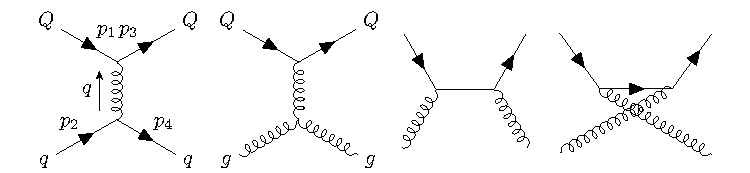
\includegraphics[width=\textwidth]{feyn-el.pdf}
\caption{Elastic processes: The first diagram corresponds to heavy quark ($Q$) - light quark ($q$, $\bar{q}$) scattering. The last three diagrams contribute to heavy quark ($Q$) - gluon ($g$) scattering.}\label{plots:feyn-elastic}
\end{figure}

\subsection{$2\rightarrow 3$ matrix-elements}
Large-Q $2\rightarrow 3$ inelastic processes are $g + i \rightarrow q+\bar{q} + i$, $q+i\rightarrow q+g+i$ and $g+i\rightarrow g+g+i$, where $i$ stands for a medium parton, and the rest symbols stands for hard parton.
In medium frame, hard parton has an energy $E\gg T$, while the medium thermal parton has $E\sim T$, and the typical center-of-mass energy is therefore $\sqrt{6ET}$.
We perform the calculation in the the center-of-mass frame of the two incoming parton and let the hard parton to be moving towards the $+z$ direction with momentum $p_1$, and the medium parton moving to the $-z$ direction with $p_2$.
The hard parton then splits into two daughter partons with momenta $k$ and $p_1 + q - k$.
The momentum transfer $q$ between the hard parton and the medium parton is thought to be large enough $|q| > Q_{\textrm{cut}}$ so we neglect the thermal correction to its propagator.

Our derivation largely follows the work \cite{Fochler:2013epa} while relaxing the soft approximation $xq_\perp \ll k_\perp$ in \cite{Fochler:2013epa}, and we only use the collinear approximation $k_\perp^2, q_\perp^2 \ll x(1-x) \hat{s}$ with $x = k^+/\sqrt{s} = k_\perp e^y_k /\sqrt{s}$.
Also, we only include the contributions with a $\hat{t}$-channel momentum exchange between the medium and the hard partons.
The collinear approximation requires $y_k \gg \ln(k_\perp/\sqrt{s})$ so that $y_k$ cannot be arbitrarily small and $y_k>0>\gg -\ln(\sqrt{s}/k_\perp)$ is a reasonable range of application.
Because $\hat{s}\sim 6 ET$, we expect this approximation to break down when either the typical values of $q_\perp^2$ becomes comparable to $x(1-x)6ET$ or when $y_k<0$ ($x < k_\perp/\sqrt{s} \sim k_\perp/\sqrt{6ET}$).
We shall briefly mention the treatment of the $y_k<0$ region in the end.

The light-cone momentum for $p_1$ , $p_2$ and $k$ can written down directly using $\sqrt{s}$, $x$ and $k_\perp$, then applying the above collinear condition, the expression for $q$ (and therefore $p_3$ and $p_4$) is obtained by kinematic constraint up to corrections of order $\{k_\perp, q_\perp^2\}/x(1-x)\hat{s}$.
\begin{eqnarray}
p_1 &=& (\sqrt{s}, 0, \vec{0})\\
p_2 &=& (0, \sqrt{s}, \vec{0})\\
k &=& (x\sqrt{s}, \frac{k_\perp^2}{x\sqrt{s}}, \vec{k}_\perp)\\
q &\sim& (-\frac{q_\perp^2}{\sqrt{s}}, \frac{q_\perp^2 + k_\perp^2/x - 
2\vec{q}_\perp \cdot \vec{k}_\perp}{(1-x)\sqrt{s}}, \vec{k}_\perp)
\end{eqnarray}
Using the light-cone gauge with a light-like vector $n = (0, 1, 0)$, the gauge fixing condition $n\cdot A =0$ eliminates the ``+" component in the gluon (with momentum $p$) polarization vector, and is obtained by applying the transverse condition $\epsilon \cdot p = 0$ (up to a higher order correction to its normalization)
\begin{eqnarray}
\epsilon(p) &\sim& (0, \frac{2\vec{\epsilon}_\perp\cdot\vec{p}_\perp}{p^+}, \vec{\epsilon}_\perp).
\end{eqnarray}
With these preparations, the matrix-element is factorized into an amplitude for the splitting process (approximated in the collinear limit) times the amplitude for two-body collision with the medium parton.
We shall only derive explicitly the cases where the medium parton is a quark, for colliding with medium anti-quark and gluon, it is sufficient to replace the $H+q\xrightarrow{\hat{t}} H+q$ amplitude by $H+\bar{q}\xrightarrow{\hat{t}} H+\bar{q}$ and $H+g\xrightarrow{\hat{t}} H+g$.
The connect of these results to the Bethe-Heitler limit of the AMY integral equation will be elucidated in the end.

\paragraph*{Gluon splitting to quark-anti-quark pair}
\begin{figure}
\centering
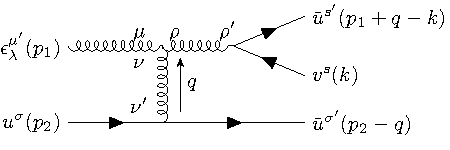
\includegraphics[width=.5\textwidth]{Large-Q-g2qqbar-A.pdf}\\
\vspace{1em}
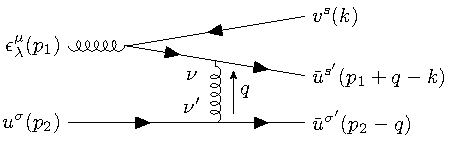
\includegraphics[width=.49\textwidth]{Large-Q-g2qqbar-B.pdf}\hfill
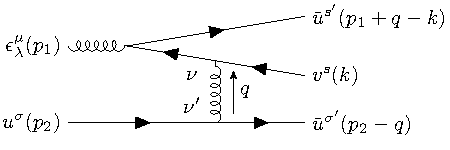
\includegraphics[width=.49\textwidth]{Large-Q-g2qqbar-C.pdf}
\caption{Three diagrams $A$ (Top), $B$ (Bottom left), $C$ (Bottom right) that contribute to the large angle scattering induced gluon splitting into quark-anti-quark pair in the forward region of the center-of-mass frame.}
\label{fig:feyn-g2qqbar}
\end{figure}

Three Feynman diagrams contribute to the kinematic region $y_k >0$ in the current approximation, as shown in figure \ref{fig:feyn-g2qqbar}.
We start from the amplitude for diagram $A$.
\begin{eqnarray}
i M_A &=& (-ig)^2(-g)f^{abc}(t^b)_{j'j}(t^c)_{i'i} \epsilon_\lambda^\mu(p_1) \\\nonumber
&&\frac{-i}{(p_1+q)^2}\left(g^{\rho\rho'}-\frac{n^{\rho}(p_1+q)^{\rho'}+n^{\rho'}(p_1+q)^\rho}{n\cdot (p_1+q)}\right) \bar{u}^s(p_1+q-k)\gamma_{\rho'}v^{s'}(k) \\ \nonumber
&&\frac{-i}{q^2}\left(g^{\nu\nu'}-\frac{n^{\nu}q^{\nu'}+n^{\nu'}q^\nu}{n\cdot q}\right) \bar{u}^{\sigma}(p_4)\gamma_{\nu'}u^{\sigma'}(p_2) \\ \nonumber
&& \left[g_{\mu\nu}(p_1-q)_\rho + g_{\nu\rho}(2q+p_1)_\rho + g_{\rho\mu}(-2p_1 -q)_\nu \right]
\end{eqnarray}
Next, express the projection matrix of the gluon propagator with momentum $p_1+q$ by the sum of tensor products of its polarization vectors, and identify the amplitude $iP_{A,\lambda'}^{ss'}$ for a gluon with polarization $\lambda'$ to split into the quark and anti-quark pair with spin $s$ and $s'$.
Also, use the high energy approximation to replace $\bar{u}^i(a)\gamma^\alpha u^j(b)$ by $(a+b)^\alpha \delta^{ij}$, then
\begin{eqnarray}
i M_A &\approx& -g^3 f^{abc}(t^b)_{j'j}(t^c)_{i'i} \delta^{\sigma\sigma'} \epsilon^\mu(p_1) \\\nonumber
&&\frac{1}{(p_1+q)^2} \sum_{\lambda'=\pm}\epsilon_{\lambda'}^{\rho}(p_1+q)\underbrace{\epsilon_{\lambda'}^{*,\rho'}(p_1+q) \bar{u}^s(p_1+q-k)\gamma_{\rho'}v^{s'}(k)}_{iP_{A,\lambda'}^{ss'}} \\ \nonumber
&&\frac{1}{q_\perp^2}\left(g^{\nu\nu'}-\frac{n^{\nu}q^{\nu'}+n^{\nu'}q^\nu}{n\cdot q}\right) (2p_2-q)_{\nu'} \\ \nonumber
&& \left[g_{\mu\nu}(p_1-q)_\rho + g_{\nu\rho}(2q+p_1)_\rho + g_{\rho\mu}(-2p_1 -q)_\nu \right] \\
&=& -g^3 f^{abc}(t^b)_{j'j}(t^c)_{i'i} \frac{1}{(p_1+q)^2}\frac{1}{q_\perp^2} \sum_{\lambda'=\pm}iP_{A,\lambda}^{ss'} \delta^{\sigma\sigma'}  \\ \nonumber
&& \epsilon_\lambda^\mu(p_1)2p_2^{\nu} \epsilon_{\lambda'}^{\rho}(p_1+q) \left[g_{\mu\nu}(p_1-q)_\rho + g_{\nu\rho}(2q+p_1)_\rho + g_{\rho\mu}(-2p_1 -q)_\nu \right].
\end{eqnarray}
Finally, we evaluate the contraction in the second line using the expression for $p_1, q$ and $\epsilon$, and keep only terms that is leading in $q_\perp^2/s$ to get,
\begin{eqnarray}
i M_A \approx -g^3 f^{abc}(t^b)_{j'j}(t^c)_{i'i}\delta^{\sigma\sigma'}\frac{2s}{q_\perp^2} \frac{x(1-x)}{(\vec{k}_\perp-x \vec{q}_\perp)^2} iP_{A,\lambda}^{ss'}.
\end{eqnarray}

Diagram B and C are similar and we only write down diagram B in detail.
\begin{eqnarray}
i M_B &=& (-ig)^3 (t^bt^a)_{i'i}(t^b)_{j'j} \epsilon_\lambda^\mu(p_1) \\\nonumber
&&\frac{-i}{q^2}\left(g^{\nu\nu'}-\frac{n^{\nu}q^{\nu'}+n^{\nu'}q^\nu}{n\cdot q}\right) \\\nonumber
&&\bar{u}^s(p_1+q-k)\gamma_{\nu}\frac{i(\slashed{p_1}-\slashed{k})}{(p_1-k)^2}\gamma^{\mu}v^{s'}(k) \\ \nonumber
&&\bar{u}^{\sigma}(p_4)\gamma_{\nu'}u^{\sigma'}(p_2)
\end{eqnarray}
Again, represent the tensor structure of the fermion propagator by the sum of tensor products of the spinors, identify the splitting amplitude $iP_{B,\lambda'}^{ss'}$ and use the high energy limit of the current,
\begin{eqnarray}
i M_B &\approx& ig^3 (t^bt^a)_{i'i}(t^b)_{j'j}  \\\nonumber
&&\frac{-i}{q_\perp^2}\left(g^{\nu\nu'}-\frac{n^{\nu}q^{\nu'}+n^{\nu'}q^\nu}{n\cdot q}\right) (2p_2-q)_\nu' \\\nonumber
&&\frac{1}{2p_1\cdot k} \sum_\sigma \bar{u}^s(p_1+q-k)\gamma_{\nu} u^{\sigma}(p_1-k) \underbrace{\epsilon_\lambda^\mu(p_1)\bar{u}^{\sigma}(p_1-k) \gamma^{\mu}v^{s'}(k)}_{iP_{B,\lambda}^{\sigma s'}}\\
&\approx& ig^3 (t^bt^a)_{i'i}(t^b)_{j'j} \frac{-i}{q_\perp^2}\frac{1}{2p_1\cdot k} iP_{B,\lambda}^{ss'}\\\nonumber
&&\left(g^{\nu\nu'}-\frac{n^{\nu}q^{\nu'}+n^{\nu'}q^\nu}{n\cdot q}\right) (2p_2-q)_{\nu'} (2p_1-q+2k)_\nu 
\end{eqnarray}
Note that $iP_{B}$ is different from $iP_{A}$ as the initial splitting parton has a different transverse momentum from diagram $A$.
Finally, evaluate the contraction and get,
\begin{eqnarray}
i M_B &=& i g^3 (t^b t^a)){i'i} t^b{j'j} \delta^{\sigma\sigma'} \frac{2s}{q_\perp^2} \frac{x(1-x)}{k_\perp^2}  iP_{B,\lambda}^{ss'}
\end{eqnarray}
Diagram C can be obtained similarly,
\begin{eqnarray}
i M_C &=& -i g^3 (t^a t^b)){i'i} t^b{j'j} \delta^{\sigma\sigma'} \frac{2s}{q_\perp^2} \frac{x(1-x)}{(\vec{k}_\perp-\vec{q}_\perp)^2}  iP_{C,\lambda}^{ss'} 
\end{eqnarray}
To sum the contributions from all three diagrams, applying $f^{abc}t^c = -i[t^a, t^b]$ to $iM_A$ and the result is,
\begin{eqnarray}
i (M_A+M_B+M_C) &=& ig^3 \frac{2s}{q_\perp^2} (t^b)_{j'j} x(1-x)\\\nonumber
&&\left\{(t^a t^b)_{i'i} \left(\frac{iP_{A,\lambda}^{ss'} }{(\vec{k}_\perp-x \vec{q}_\perp)^2} - \frac{iP_{C,\lambda}^{ss'}}{(\vec{k}_\perp-\vec{q}_\perp)^2}\right) \right. \\\nonumber
&&\left.-(t^a t^b)_{i'i}\left(\frac{iP_{A,\lambda}^{ss'} }{(\vec{k}_\perp-x \vec{q}_\perp)^2} - \frac{iP_{B,\lambda}^{ss'}}{k_\perp^2}\right) \right\}
\end{eqnarray}

Now we have to address what those splitting amplitudes are.
Label the four momenta as $p_g = c$, $p_q = a$, $p_{\bar{q}} = b$.
And use the following representation for the spinors,
\begin{eqnarray}
u^s(p) = (\sqrt{p\cdot \sigma} \xi^s, \sqrt{p\cdot \bar{\sigma}} \xi^s)^T
v^s(p) = (\sqrt{p\cdot \sigma} \eta^s, -\sqrt{p\cdot \bar{\sigma}} \eta^s)^T
\end{eqnarray}
where $\sigma_{i=\{1,2,3\}}$ are Pauli matrices, $\sigma = (1_{2\times 2}, \vec{\sigma})$, and $\bar{\sigma} = (1_{2\times 2}, -\vec{\sigma})$.
The square root of the matrix is,
\begin{eqnarray}
\sqrt{p\cdot \sigma} =
\left.
\begin{bmatrix}
p^- & -p_L^\perp \\
-p_R^\perp & p^+
\end{bmatrix}\right.^{1/2} 
= \frac{1}{\sqrt{2(E\pm M)}}(p\cdot\sigma \pm \mathbf{1}M)\\
\sqrt{p\cdot \bar{\sigma}} =
\left.
\begin{bmatrix}
p^+ & p_\perp^- \\
p_R^\perp & p^-
\end{bmatrix}\right.^{1/2} 
= \frac{1}{\sqrt{2(E\pm M)}}(p\cdot\bar{\sigma} \pm \mathbf{1}M)\\
\end{eqnarray}
where $M$ is the mass of the particle, $p^\pm = E\pm p_z$, and $p_{R,L}^\perp = p_x \pm  i p_y$.
Currently, we only consider the massless case, because the mass effect is not implemented in the few-body matrix-elements in our model.
Neglecting the mass, the splitting amplitude is,
\begin{eqnarray}
&&\epsilon_{\lambda, \mu}(c) \bar{u}_s(a)\gamma^\mu v_{s'}(b)\\
&=&\frac{1}{\sqrt{2a}\sqrt{2b}}(\xi^T_s a\cdot\sigma, \xi^T_{s} a\cdot \bar{\sigma})
\begin{bmatrix}
\epsilon\cdot\bar{\sigma} & 0 \\
0 & \epsilon\cdot\sigma
\end{bmatrix}
\begin{bmatrix}
b\cdot\sigma \eta_{s'}\\
b\cdot\bar{\sigma} \eta_{s'}
\end{bmatrix}
\\
&=&\frac{1}{2\sqrt{ab}}
\xi_s^T
\begin{bmatrix}
a^- & -a^\perp_L \\
-a^\perp_R & a^+
\end{bmatrix}
\begin{bmatrix}
0 & \sqrt{2}\delta_{\lambda R}\\
\sqrt{2}\delta_{\lambda L} & \frac{\sqrt{2}c^\perp_\lambda}{c^+}
\end{bmatrix}
\begin{bmatrix}
b^- & -b^\perp_L \\
-b^\perp_R & b^-
\end{bmatrix}
\eta_{s'}\\\nonumber
&-&
\frac{1}{2\sqrt{ab}}
\xi_s^T
\begin{bmatrix}
a^+ & a^\perp_L \\
a^\perp_R & a^-
\end{bmatrix}
\begin{bmatrix}
\frac{\sqrt{2}c^\perp_\lambda}{c^+} & -\sqrt{2}\delta_{\lambda R}\\
-\sqrt{2}\delta_{\lambda L} & 0
\end{bmatrix}
\begin{bmatrix}
b^+ & b^\perp_L \\
b^\perp_R & b^-
\end{bmatrix}
\eta_{s'}
\\
&=&\frac{1}{\sqrt{2ab}}
\xi_s^T
\begin{bmatrix}
-a^\perp_L b^- \delta_{\lambda L} - a^- b^\perp_L \delta_{\lambda R} + a^\perp_L b^\perp_R\frac{c^\perp_\lambda}{c^+} &
a^\perp_L b^\perp_L \delta_{\lambda L} + a^- b^+ \delta_{\lambda R} - a^\perp_L b^+\frac{c^\perp_\lambda}{c^+}
\\
a^+ b^- \delta_{\lambda L} + a^\perp_R b^\perp_R \delta_{\lambda R} - a^+ b^\perp_R\frac{c^\perp_\lambda}{c^+} &
-a^+ b^\perp_L \delta_{\lambda L} - a^\perp_R b^+ \delta_{\lambda R} + a^+ b^+\frac{c^\perp_\lambda}{c^+}
\end{bmatrix}
\eta_{s'}\\\nonumber
&-&\frac{1}{\sqrt{2ab}}
\xi_s^T
\begin{bmatrix}
-a^\perp_L b^+ \delta_{\lambda L} - a^+ b^\perp_R \delta_{\lambda R} + a^+ b^+\frac{c^\perp_\lambda}{c^+} &
-a^\perp_L b^\perp_L \delta_{\lambda L} - a^+ b^- \delta_{\lambda R} + a^+ b^\perp_L\frac{c^\perp_\lambda}{c^+}
\\
-a^- b^+ \delta_{\lambda L} - a^\perp_R b^\perp_R \delta_{\lambda R} + a^\perp_+ b^+\frac{c^\perp_\lambda}{c^+} &
-a^- b^\perp_L \delta_{\lambda L} - a^\perp_R b^- \delta_{\lambda R} + a^\perp_R b^\perp_L\frac{c^\perp_\lambda}{c^+}
\end{bmatrix}
\eta_{s'}
\end{eqnarray}
Keep the leading terms in the collinear limit which are products of $(+)(+)$ or $(+)(\perp)$ components of the momenta, and drop terms that are of order $(+)(-)$, $(\perp)(\perp)$ and $(\perp)(-)$,
\begin{eqnarray}
&&\epsilon_{\lambda, \mu} \bar{u}_s(a)\gamma^\mu v_{s'}(b)\\
&=& \frac{1}{\sqrt{2ab}}
\xi_s^T
\begin{bmatrix}
a^\perp_L b^+ \delta_{\lambda L} + a^+ b^\perp_R \delta_{\lambda R} - a^+ b^+\frac{c^\perp_\lambda}{c^+} & 0\\
0 & -a^+ b^\perp_L \delta_{\lambda L} - a^\perp_R b^+ \delta_{\lambda R} + a^+ b^+\frac{c^\perp_\lambda}{c^+}
\end{bmatrix}
\eta_{s'}
\end{eqnarray}
There are four combinations for the possible initial state polarization and final state spins
\begin{eqnarray}
\epsilon_{\lambda, \mu} \bar{u}_s(a)\gamma^\mu v_{s'}(b) = \frac{x\vec{a} - (1-x)\vec{b}}{\sqrt{2x(1-x)}}
\begin{cases}
x, \hfill \lambda=L, s=\uparrow\\
-(1-x), \hfill \lambda=L, s=\downarrow\\
(1-x), \hfill \lambda=R, s=\uparrow\\
-x, \hfill \lambda=R, s=\downarrow\\
\end{cases}
\end{eqnarray}
Where we have use $a^+ = (1-x)c^+, b^+ = xc^+$ and $c_\perp = a_\perp+b_\perp$.
Sum over the spins and average over polarization for the squared amplitude,
\begin{eqnarray}
\frac{1}{2}\sum_\pm |P|^2 = \frac{2(x^2 + (1-x)^2)}{x(1-x)} \left((1-x)\vec{a}_\perp-x\vec{b}_\perp\right)^2.
\end{eqnarray}
This result goes back to the standard splitting function if it is computed in the frame where $a_\perp = -b_\perp$. 
However, there is no such frame that $a_\perp = -b_\perp$ satisfies simultaneously for the splitting in diagram A, B and C, therefore different amplitude needs to be inserted for each diagram and we find,
\begin{eqnarray}
\frac{\sum_{\lambda, s, s', \sigma, \sigma', a, b}|M^2|_{g+q\rightarrow q+\bar{q}+q}}{2d_F 2d_A} &=& g^4 \frac{2C_F}{d_A}\frac{4s^2 x(1-x)}{q_\perp^4}  \\\nonumber
&\times& g^2\frac{(x^2+(1-x)^2)}{2} \left(C_F \vec{A}^2 + C_F \vec{B}^2 - (2C_F- C_A)\vec{A}\cdot\vec{B}\right)
\end{eqnarray}
Where the $\vec{A}$ and $\vec{B}$ is,
\begin{eqnarray}
\vec{A} &=& \frac{\vec{k}_\perp - x\vec{q}_\perp}{(\vec{k}_\perp - x\vec{q}_\perp)^2} -  \frac{\vec{k}_\perp - \vec{q}_\perp}{(\vec{k}_\perp - \vec{q}_\perp)^2}, \\
\vec{B} &=& \frac{\vec{k}_\perp - x\vec{q}_\perp}{(\vec{k}_\perp - x\vec{q}_\perp)^2} -  \frac{\vec{k}_\perp}{\vec{k}_\perp^2}.
\end{eqnarray}
The final squared matrix-element has been factorized into the two body scattering part (first line) and the collinear splitting part (second line) with the desired leading order QCD splitting function. 

\paragraph*{Quark splits to quark and gluon}
\begin{figure}
\centering
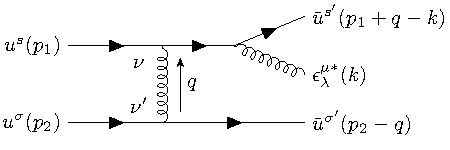
\includegraphics[width=.5\textwidth]{Large-Q-q2qg-A.pdf}\\
\vspace{1em}
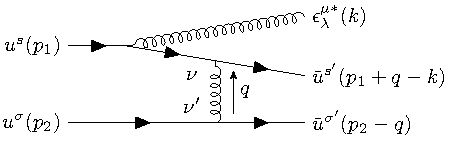
\includegraphics[width=.49\textwidth]{Large-Q-q2qg-B.pdf}\hfill
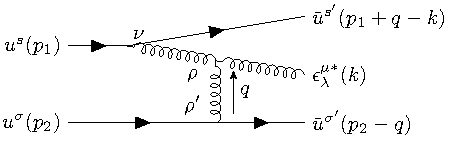
\includegraphics[width=.49\textwidth]{Large-Q-q2qg-C.pdf}
\caption{Three diagrams $A$ (Top), $B$ (Bottom left), $C$ (Bottom right) that contribute to the large angle scattering induced a quark splitting into a quark and a gluon in the forward region of the center-of-mass frame.}
\label{fig:feyn-q2qg}
\end{figure}

The Feynman diagrams to be included for $q+q\rightarrow q+g+q$ are shown in Figure \ref{fig:feyn-q2qg}.
The calculation uses exactly the same technique we used for the gluon splitting channel, and we present the result directly,
\begin{eqnarray}
\overline{|M^2|}_{g+q\rightarrow g+g+q} &=& 
 g^4 \frac{C_F}{d_F}\frac{4s^2}{q_\perp^4}x(1-x) \\\nonumber
&\times&g^2\frac{1+(1-x)^2}{x}  
\left(C_F\vec{A}^2 + C_F\vec{B}^2 - \left(2C_F-C_A\right)\vec{A}\cdot\vec{B}\right)\\
\vec{A} &=& \frac{\vec{k}_\perp - \vec{q}_\perp}{(\vec{k}_\perp - \vec{q}_\perp)^2} -  \frac{\vec{k}_\perp - x\vec{q}_\perp}{(\vec{k}_\perp - x\vec{q}_\perp)^2} \\
\vec{B} &=& \frac{\vec{k}_\perp - \vec{q}_\perp}{(\vec{k}_\perp - \vec{q}_\perp)^2} -  \frac{\vec{k}_\perp}{\vec{k}_\perp^2}
\end{eqnarray}


\paragraph*{Gluon splitting to two gluons}
\begin{figure}
\centering
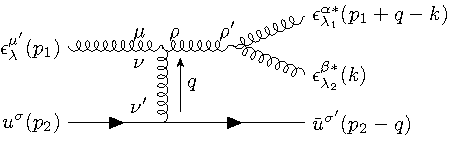
\includegraphics[width=.5\textwidth]{Large-Q-g2gg-A.pdf}\\
\vspace{1em}
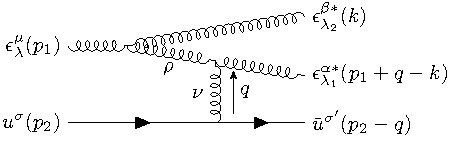
\includegraphics[width=.49\textwidth]{Large-Q-g2gg-B.pdf}\hfill
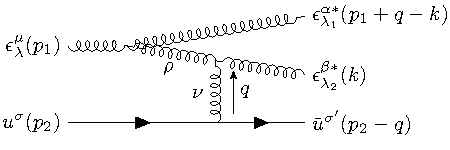
\includegraphics[width=.49\textwidth]{Large-Q-g2gg-C.pdf}
\caption{Three diagrams $A$ (Top), $B$ (Bottom left), $C$ (Bottom right) that contribute to the large angle scattering induced gluon splitting into two gluons in the forward region of the center-of-mass frame.}
\label{fig:feyn-g2gg}
\end{figure}

Finally, for $g+q\rightarrow g+q+g$, the Feynman diagrams are shown in Figure \ref{fig:feyn-g2gg}. 
The simplification of the two body collision amplitude can be done in a similar manner as the previous two channels. 
We only write down the splitting amplitude $g\rightarrow g+ g$ in detail.
Suppressing the color index, we label the initial gluon with $\epsilon_1^\mu(p)$, and the two daughter gluons with $\epsilon_2^\nu(k)$ and $\epsilon_3^\rho(q)$.
The splitting amplitudes are then (omitting the factor $-gf^{abc}$)
\begin{eqnarray}
iP &=& \epsilon^\mu_1\epsilon^\nu_2\epsilon^\rho_3
\left[
g_{\mu\nu} (p+k)_{\rho} +  g_{\nu\rho} (p+k)_{\mu} + g_{\rho\mu} (-q-p)_{\nu}
\right]\\
&=& -\vec{\epsilon}_{1,\perp}\cdot \vec{\epsilon}_{2,\perp} \left[(p+k)^+\frac{\vec{\epsilon}_{3,\perp}\cdot \vec{q}_\perp}{q^+} - \vec{\epsilon}_{3,\perp}\cdot (\vec{p}_\perp+\vec{k}_\perp)\right] \\\nonumber
&&-\vec{\epsilon}_{2,\perp}\cdot \vec{\epsilon}_{3,\perp} \left[(-k+q)^+\frac{\vec{\epsilon}_{1,\perp}\cdot \vec{p}_\perp}{p^+} - \vec{\epsilon}_{1,\perp}\cdot (-\vec{k}_\perp+\vec{q}_\perp)\right]
\\\nonumber
&&-\vec{\epsilon}_{3,\perp}\cdot \vec{\epsilon}_{1,\perp} \left[(-q-p)^+\frac{\vec{\epsilon}_{2,\perp}\cdot \vec{k}_\perp}{k^+} - \vec{\epsilon}_{2,\perp}\cdot (-\vec{q}_\perp-\vec{p}_\perp)\right]
\end{eqnarray}
There are four possible combinations of the polarization vectors, and their respective amplitude is computed as,
\begin{eqnarray}
iP = \sqrt{2}\left[x\vec{q}_\perp - (1-x)\vec{k}_\perp\right]\times 
\begin{cases}
\frac{1-x+x^2}{x(1-x)}, \hfill \lambda_1=\lambda_2=\lambda_3\\
-1, \hfill \lambda_1\neq\lambda_2=\lambda_3 \\
\frac{1}{x}, \hfill \lambda_1=\lambda_3\neq\lambda_2\\
\frac{1}{1-x}, \hfill \lambda_1=\lambda_2\neq\lambda_3
\end{cases}
\end{eqnarray}
Summing over the squared amplitude of all four cases and average over the initial gluon polarization, one gets the desired leading order QCD splitting function,
\begin{eqnarray}
2\frac{1+x^2+(1-x)^4}{x^2(1-x)^2} \left[x\vec{q}_\perp - (1-x)\vec{k}_\perp\right]^2.
\end{eqnarray}

Substitute the the amplitude in each diagram, the final squared matrix-element is 
\begin{eqnarray}
\overline{|M^2|}_{g+q\rightarrow g+g+q} &=&
g^4 \frac{C_A}{d_F}\frac{4s^2x(1-x)}{q_\perp^4} \\\nonumber
&\times&g^2\frac{1+x^4+(1-x)^4}{x(1-x)}   
\left(C_A\vec{A}^2 + C_A\vec{B}^2 - C_A\vec{A}\cdot\vec{B}\right)\\
\vec{A} &=& \frac{\vec{k}_\perp - x\vec{q}_\perp}{(\vec{k}_\perp - x\vec{q}_\perp)^2} -  \frac{\vec{k}_\perp - \vec{q}_\perp}{(\vec{k}_\perp - \vec{q}_\perp)^2} \\
\vec{B} &=& \frac{\vec{k}_\perp - x\vec{q}_\perp}{(\vec{k}_\perp - x\vec{q}_\perp)^2} -  \frac{\vec{k}_\perp}{\vec{k}_\perp^2}
\end{eqnarray}

\paragraph{Regulating the $2\rightarrow 3$ squared matrix-elements}
The divergence in the $q$ integration is removed by the requirement that this few-body matrix-element only applies to processes with $q>Q_{\textrm{cut}}$.
The collinear divergence when $k$ approaching $q$, $xq$ is regulated by including a gluon thermal mass. 
In practice, these collinear region will be further suppressed by the LPM effect.
The cross-section is obtained by integrating over the final state phase-space, where we have chosen to parameterize the three particle final state in terms of $k_\perp^2$, the rapidity of $k$ in the center-of-mass frame $y_k$, and the solid angle of the recoil medium particle.

\paragraph{Soft limit: the Gunion-Bertsch approximation}
The result we obtained for the $g\rightarrow g+g$ and $q\rightarrow q+g$ channel has a soft limit that goes back to the well known Gunion-Bertsch form. 
By soft limit, we require the radiated gluon energy to be small enough such that $xq_\perp \ll k_\perp$.
Then, the splitting amplitudes for both $g\rightarrow g+g$ and  $q\rightarrow q+g$ are simplified into the same form,
\begin{eqnarray}
\overline{|M|}^2_{22} x(1-x)g^2 \frac{2(1-x+O(x^2))}{x} C_A \left(\frac{\vec{k}_\perp}{k_\perp^2}-\frac{\vec{k}_\perp-\vec{q}_\perp}{(\vec{k}_\perp-\vec{q}_\perp)^2}\right)^2
\end{eqnarray}
Neglecting the $O(x^2)$ terms in the splitting function, the result is the same as the improved verison of the Gunion-Bertsch cross-section \cite{Fochler:2013epa} used in the full Boltzmann partonic transport model BAMPS \cite{Xu:2004mz},
\begin{eqnarray}
\overline{|M|}^2_{22} 8\pi C_A\alpha_s (1-x)^2 \left(\frac{\vec{k}_\perp}{k_\perp^2}-\frac{\vec{k}_\perp-\vec{q}_\perp}{(\vec{k}_\perp-\vec{q}_\perp)^2}\right)^2
\end{eqnarray}

\paragraph{The backward ($y_k < 0$) region}
We have mentioned in the beginning of the derivation that the condition $k_\perp^2 < x(1-x)\hat{s}$ restricts the splitting to be happen only for the parton moving in the $+z$ direction in the center-of-mass frame ($y_k > 0$).
For splitting that happens in the backward region, another set of diagrams contributes, where the splitting comes from the parton that moves in the $-z$ direction in the center-of-mass frame.
Also one needs a different gauge $A^- = 0$.
The derivation is similar to the previous ones, but with the definition of $x$ and $q$ changed to $x = k^-/\sqrt{s}$, and $q = p_1-p_3$.

To combine the results that is obtained in different regions of phase space ($y_k > 0$ and $y_k < 0$), we follow \cite{Fochler:2013epa} and defines,
\begin{eqnarray}
\bar{x} &=& \frac{(k + |k_z|)}{\sqrt{s}} = \frac{k_\perp e^{|y_k|}}{\sqrt{s}}\\ 
\bar{q} &=& \Theta(y_k)(p_2-p_4) + \Theta(-y_k)(p_1-p_3)
\end{eqnarray}
which replaces the original $x$ and $q$ in our formula, and the resultant matrix-elements can be used for both forward and backward regions.

\paragraph*{Relation to the Bethe-Heitler limit of the AMY formalisim}
Now we show the connection between the $2\rightarrow 3$ cross section obtained here and the Bethe-Heitler limit of the AMY equation.
In the Bethe-Heitler limit, the AMY integral equation can be solved approximately by treating $1/\tau_f$ as the leading factor. 
One get the splitting rate for each different channels (denoting $\vec{a}/a^2$ as $\vec{\phi}_{a}$), 
\begin{eqnarray}
R_{q\rightarrow q+g}^{BH} &\propto& g^2 P_{qg}^{q(0)}(x) \int d k^2 d q^2 \mathcal{A}(q^2) \left\{
C_A\vec{\phi}_k\cdot\left(\vec{\phi}_k-\vec{\phi}_{k-q}\right) \right.\\\nonumber
&&+\left. (2C_F-C_A) \vec{\phi}_k\cdot\left(\vec{\phi}_k-\vec{\phi}_{k+xq}\right)
+ C_A \vec{\phi}_k\cdot\left(\vec{\phi}_k - \vec{\phi}_{k+(1-x)q}\right)
\right\}
\\
R_{g\rightarrow g+g}^{BH} &\propto& g^2 P_{gg}^{g(0)}(x) \int d k^2 d q^2 \mathcal{A}(q^2) \left\{
C_A\vec{\phi}_k\cdot\left(\vec{\phi}_k-\vec{\phi}_{k-q}\right) \right.\\\nonumber
&&+\left. C_A \vec{\phi}_k\cdot\left(\vec{\phi}_k-\vec{\phi}_{k+xq}\right)
+ C_A \vec{\phi}_k\cdot\left(\vec{\phi}_k - \vec{\phi}_{k+(1-x)q}\right)
\right\}
\\
R_{g\rightarrow q+\bar{q}}^{BH} &\propto& g^2 P_{q\bar{q}}^{g(0)}(x) \int d k^2  d q^2 \mathcal{A}(q^2) \left\{
(2C_F-C_A)\vec{\phi}_k\cdot\left(\vec{\phi}_k-\vec{\phi}_{k-q}\right) \right.\\\nonumber
&&+\left. C_A \vec{\phi}_k\cdot\left(\vec{\phi}_k-\vec{\phi}_{k+xq}\right)
+ C_A \vec{\phi}_k\cdot\left(\vec{\phi}_k - \vec{\phi}_{k+(1-x)q}\right)
\right\}
\end{eqnarray}
with the collision kernel $\mathcal{A} = g^2 T m_D^2/q^2(q^2+m_D^2)$. These expression looks drastically different from the incoherent rate computed using the cross-section derived in the previous section, however, we would like to show that they are the same once integration over $dk^2$ is performed.
Therefore, the incoherent rate we used in the Boltzmann equation indeed recover the Bethe-Heitler limit of the AMY integral equation.

To show this, we start from the $2\rightarrow 3$ rate formula using the matrix-elements from equation. 
Starting from the $q\rightarrow q+g$ channel, the rate in our Boltzmann equation is,
\begin{eqnarray}
R_{q\rightarrow q+g} &\propto& g^2 P_{qg}^{q(0)}(x) \int  \frac{f(p_2)dp_2^3}{2E_2(2\pi)^3} d q^2 \frac{g^4}{q^4}\\\nonumber
&&  \int d k^2\left\{
C_F\left( \vec{\phi}_{k-q}-\vec{\phi}_{k-xq} \right)^2
+ C_F\left( \vec{\phi}_{k-q}-\vec{\phi}_{k} \right)^2\right.\\\nonumber
&&\left.
- (2C_F-C_A)\left( \vec{\phi}_{k-q}-\vec{\phi}_{k-xq} \right)\cdot \left( \vec{\phi}_{k-q}-\vec{\phi}_{k} \right)
\right\}
\end{eqnarray}
Focusing on the three products (squares) of $\vec{\phi}$s under the $dk^2$ integration, we are going to expand the first term in each product and then shift the argument of the first $\vec{\phi}$ to $k$, 
\begin{eqnarray}
R_{q\rightarrow q+g} &\propto& g^2 P_{qg}^{q(0)}(x) \int  \frac{f(p_2)dp_2^3}{2E_2(2\pi)^3} d q^2 \frac{g^4}{q^4}\\\nonumber
&&  \int d k^2\left\{
C_F\vec{\phi}_{k}\left( \vec{\phi}_{k}-\vec{\phi}_{k+(1-x)q} \right)
- C_F\vec{\phi}_{k}\left( \vec{\phi}_{k-(1-x)q}-\vec{\phi}_{k} \right)\right.
\\\nonumber
&&+ C_F\vec{\phi}_{k}\left( \vec{\phi}_{k}-\vec{\phi}_{k+q} \right)
- C_F\vec{\phi}_{k}\left( \vec{\phi}_{k-q}-\vec{\phi}_{k} \right)
\\\nonumber
&&\left.
- (2C_F-C_A)\vec{\phi}_{k}\cdot \left( \vec{\phi}_{k}-\vec{\phi}_{k+q} \right)
+(2C_F-C_A)\vec{\phi}_{k} \cdot \left( \vec{\phi}_{k-(1-x)q}-\vec{\phi}_{k+xq} \right)
\right\}
\end{eqnarray}
Next, flip  the sign of $q$ under the integration,
and meanwhile, insert a $-\vec{\phi}_k +\vec{\phi}_k$ in the brackets of the last term,
\begin{eqnarray}
R_{q\rightarrow q+g} &\propto& g^2 P_{qg}^{q(0)}(x) \int  \frac{f(p_2)dp_2^3}{2E_2(2\pi)^3} d q^2 \frac{g^4}{q^4}\\\nonumber
&&  \int d k^2\left\{
2C_F\vec{\phi}_{k}\left( \vec{\phi}_{k}-\vec{\phi}_{k+(1-x)q} \right)
+ 2C_F\vec{\phi}_{k}\left( \vec{\phi}_{k}-\vec{\phi}_{k+q} \right)
\right.
\\\nonumber
&&
- (2C_F-C_A)\vec{\phi}_{k}\cdot \left( \vec{\phi}_{k}-\vec{\phi}_{k+q} \right)
+(2C_F-C_A)\vec{\phi}_{k} \cdot \left( \vec{\phi}_{k+(1-x)q} -\vec{\phi}_k \right) \\\nonumber
&&\left.+(2C_F-C_A)\vec{\phi}_{k} \cdot \left(\vec{\phi}_k-\vec{\phi}_{k+xq} \right)
\right\}
\end{eqnarray}
After this manipulation, the first (second) term cancels the $C_F$ part of the fourth (third) term, 
\begin{eqnarray}
R_{q\rightarrow q+g} &\propto& g^2 P_{qg}^{q(0)}(x) \int  \frac{f(p_2)dp_2^3}{2E_2(2\pi)^3} d q^2 \frac{g^4}{q^4}\\\nonumber
&&  \int d k^2\left\{
C_A\vec{\phi}_{k}\cdot \left( \vec{\phi}_{k}-\vec{\phi}_{k+q} \right)
+C_A\vec{\phi}_{k} \cdot \left( \vec{\phi}_k - \vec{\phi}_{k+(1-x)q}\right) \right.\\\nonumber
&&\left.+(2C_F-C_A)\vec{\phi}_{k} \cdot \left(\vec{\phi}_k-\vec{\phi}_{k+xq} \right)
\right\}
\end{eqnarray}
which is the same integration as the one obtained from the Bethe-Heitler limit of the AMY equation (neglecting the screen mass in $\mathcal{A}$ when $q^2 \gg m_D^2$)
The equivalence between these two expressions of the $g\rightarrow g+g$ channel and the $g\rightarrow q+\bar{q}$ channel can also be shown similarly.

\paragraph*{Mass effect in the $2\rightarrow 3$ squared matrix-elements}
For completeness, we briefly outline the derivation of $2\rightarrow 3$ cross-section with mass effect.
As a remark, putting heavy flavor mass directly into the these matrix-elements are certainly legitimate if one only focus on $2\rightarrow 3$ processes.
But once we want to approximate the effect of multiple scatterings:
$(n \rightarrow n+1) \approx (2 \rightarrow 3)(2 \rightarrow 2)\cdots(2 \rightarrow 2)\times \textrm{corrections}$, it is not advantages to put the mass effect into the $(2 \rightarrow 3)$ part, but into the last step of corrections, which is the approach we used.


First, we still work under the assumption that $M \ll E$, and will only keep terms when $M$ is making direct comparison to $k_\perp, q_\perp$.
The kinematics are now changed to,
\begin{eqnarray}
p_1 &=& (\sqrt{s}, 0, \vec{0})\\
p_2 &=& (0, \sqrt{s}, \vec{0})\\
k &=& (x\sqrt{s}, \frac{k_\perp^2}{x\sqrt{s}}, \vec{k}_\perp)\\
q &\sim& (-\frac{q_\perp^2\sqrt{s}}{s-M^2}, \frac{x(\vec{q}_\perp-\vec{k}_\perp)^2 + (1-x)k_\perp^2 + x^2M^2}{x(1-x)\sqrt{s}}, \vec{k}_\perp)
\end{eqnarray}
For the splitting amplitude, off diagonal elements of $\epsilon_{\lambda, \mu}(c) \bar{u}_s(a) \gamma^\mu v_{s'} (b)$ also needs to be included for helicity flipping process. 
Moreover,
\begin{eqnarray}
\sqrt{p\cdot \sigma} &=& \frac{p\cdot \sigma + M}{\sqrt{2(E+M)}} \approx \frac{p\cdot \sigma + M}{\sqrt{2E}} \\
\sqrt{p\cdot \bar{\sigma}} &=& \frac{p\cdot \bar{\sigma} + M}{\sqrt{2(E+M)}} \approx \frac{p\cdot \bar{\sigma} + M}{\sqrt{2E}}
\end{eqnarray}
where we have omitted the mass in the denominator since it only involves corrections of order $M/E$.
From this one can see that the previous calculation can be used for the massive case with the substitution  $a^\pm \rightarrow a^\pm +M$ and $b^\pm \rightarrow b^\pm +M$.
Then, the splitting amplitude becomes,
\begin{eqnarray}
\epsilon_{\lambda, \mu} \bar{u}_s(a)\gamma^\mu v_{s'}(b)&=& \frac{1}{\sqrt{2ab}}
\xi_s^T A_{ss'} \eta_{s'}\\
A_{\uparrow\uparrow} &=&
\delta_{\lambda L} 2b_z a^\perp_L + \delta_{\lambda R} 2a_z b^\perp_R + \frac{c^\perp_\lambda}{c^+} (a^\perp_L b^\perp_R - a^+ b^+) \\
A_{\downarrow\downarrow} &=&
-\delta_{\lambda L}2a_z b^\perp_L - \delta_{\lambda R}2b_z a^\perp_R - \frac{c^\perp_\lambda}{c^+} (a^\perp_R b^\perp_L - a^+ b^+) \\
A_{\uparrow\downarrow} &=&
\delta_{\lambda L} 2a^\perp_L b^\perp_L + \delta_{\lambda R} (a^+b^-+a^-b^+) - \frac{c^\perp_\lambda}{c^+} (a^+b^\perp + a^\perp b^+) \\
A_{\downarrow\uparrow} &=&
 \delta_{\lambda L} (a^+b^-+a^-b^+) + \delta_{\lambda L} 2a^\perp_R b^\perp_R - \frac{c^\perp_\lambda}{c^+} (a^+b^\perp + a^\perp b^+) 
\end{eqnarray}


\chapter{Comprehensive heavy-flavor simulation framework}
\label{chapter:coupling}
The simulation framework for heavy flavor particles is summarized in the follow chart in figure \ref{fig:flowchart}.
The soft initial condition model provide both the initial energy density of the medium and the transverse location of the hard vertices, while pQCD based calculations initialize the momentum space of the hard partons.
The left branch of this flow chart -- the hydrodynamic-based medium evolution model -- in chapter \ref{chapter:simulation}.
We briefly review of the right branch -- the mutli-stage model for heavy-falvor.
The hard production model is introduced in section \ref{section:hard}.
The initially produced partons are highly virtual and undergo the DGLAP evolution (vacuum shower) that bring down the virtuality; eventually at some point this evolution will be matched to the in-medium transport calculations.
There is a complication for vacuum-like parton shower in a medium, since  certain vacuum parton branchings would have occupied the same space-time as the medium and also receives medium corrections.
Another obstacle is that multiple emissions are treated very differently between vacuum-like shower and medium-induce shower.
For the vacuum evolution, the ``time'' variable is the virtuality scale with the space-time information integrated out, while the transport model evolves the systems in real time, with virtuality integrated out below a certain scale.
There are many recent progress in both theory developments and newly design event-generators to solve this problem \cite{MehtarTani:2012cy,Mehtar-Tani:2017ypq,Cao:2017zih,Kauder:2018cdt,Putschke:2019yrg,PhysRevLett.120.232001,Caucal:2018ofz}.
In section \ref{section:match}, we discuss a possible prescription to interface the two types of showers in our simulation.
Section \ref{section:couple-to-hydro} contains the details of coupling the transport model to a dynamically evolving medium with large longitudinal expansion.
The heavy flavor hadronization model and hadronic rescatterings are introduced in section \ref{section:hadronization}.
The hadronization routine applies a previously implementation \cite{Cao:2013ita} of the high-$p_T$ fragmentation plus low-$p_T$ recombination model for heavy hadrons production \cite{Oh:2009zj}.
Finally, in section \ref{section:benchmark}, the model is benchmarked using a few choices of fixed coupling constant and running coupling constants, before being systematically tuned to data in the next chapter.
\begin{figure}
\centering
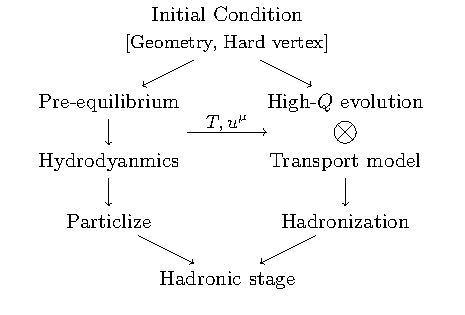
\includegraphics[width=.8\textwidth]{flowchart.pdf}
\caption{A schematic workflow of the heavy quark simulation. The left branch evolves the medium in the hydrodynamic based model, providing medium information (temperature, flow velocity) to the hard probe transport in the right branch. The hard and soft hadrons are evolved in the hadronic afterburner in the last step.}
\label{fig:flowchart}
\end{figure}

\section{Initial production of heavy flavor}
\label{section:hard}
\subsection{Factorization framework in proton-proton collisions}
In the proton-proton collision, the hard processes can be computed using the pQCD-based techniques.
The foundation of this calculation is the factorization framework as schematically demonstrated in \ref{fig:factorization}.
First, the incoming proton is a composite object and there is a certain ``probability'' of finding a parton $i(j)$ carrying $x_i(x_j)$ fraction of the momentum of the proton $p_1(p_2)$.
This ``probability'' is known as the parton distribution function (PDF) $f_i(x, Q^2)$.
It not only is a function of $x$, but also depends on the scale $Q^2$ at which the proton is probed.
The probing scale is required to be much greater than the non-perturbative scale.
Because $\alpha_s(Q^2)$ is samll due to asymptotic freedom, the process of partons $i$ and $j$ scatterings into partons $k$ and $l$ is computable in perturbative QCD.
The sinal states partons eventually produce a bunch of hadrons, which is non-perturbative process.
The parton fragmentation function is then defined as the probability to find a certain hadron $H$ carrying a fraction $x_H$ of the parton's momentum.
Combing these pieces together, the cross-section for the inclusive production of hadron can be written as \cite{Field:1989uq},
\begin{eqnarray}
\frac{d\sigma_{p+p\rightarrow H+X}}{dy d\mathbf{p}_T^2} = \frac{1}{\pi}\int dx_i dx_j f_i(x_i, Q^2) f_j(x_j, Q^2) \frac{d\sigma_{ij\rightarrow kl}}{d\hat{t}} \frac{1}{z_k}D^H(z_k, Q^2).
\end{eqnarray}
Although the parton distribution function $f$ and the parton fragmentation function $D$ are essentially non-perturbative objects, they parametrizes universal long-distance physics and can be extracted from independent experiments at certain scales $Q_0^2$.
Moreover, the evolution from their ``definition'' scale $Q_0^2$ to the process scale $Q^2$ can be described by the DGLAP evolution equation \cite{Gribov:1972ri,Altarelli:1977zs,Dokshitzer:1977sg} based on perturbative QCD to increase the predictive power of the factorization formula.

\begin{figure}
\centering
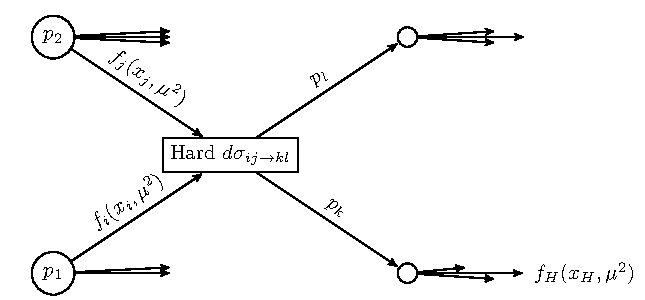
\includegraphics[width=.8\textwidth]{factorization.pdf}
\caption{A schematic demonstration of the factorization theorem. Two incoming proton momenta are $p_1$ and $p_2$. $f_{i,j}$ are the parton distribution function. $d\sigma$ is the perturbative matrix-element. $f_H$ is the fragmentation function.}
\label{fig:factorization}
\end{figure}

The DGLAP evolution takes into account that the initial high-virtuality parton $i$ (or $j$) could have come from a splitting process of a parton with lower virtuality parton $i'$ (or $j'$).
Similarly, the final state high virtuality parton $k$ (or $l$) could also split into a low virtuality parton $k'$ (or $l'$) before it turns into a hadron.
Though each splitting causes an additional power of $\alpha_s$, it is also magnified by a potentially large factor $\ln Q^2/\mu^2$ when the $Q^2$ is much greater than the scale where the $f$, $D$ are defined.
The same argument also applies to partons $i', j', k', l'$. 
The DGLAP equations systematically resum contributions including an arbitrary number of parton splittings and evolve the scale from $\mu^2$ to the hard scale $Q^2$.
Moreover, a very useful parton-shower picture can be built from this process and with a probabilistic interpretation of the DGLAP evolution. Using Monte Carlo technique, one can even mimic the exclusive final states from the sequence of parton branching processes.

\subsection{Production in the nuclear environment}
The above framework explains very well explains the hard process production in the proton-proton collisions.
In the nuclear environment, there are several differences.
First, the parton distribution function inside a nuclei is different from the superposition of the nucleons.
The ratio between nuclear PDF and proton PDF generally deviates from unity.
In particular, this ratio for small $x$ gluon is significantly below one, known as the nuclear shadowing effect. 
This ratio increase and become larger than one at larger $x$, termed as the anti-shadowing region.
The difference between the nuclear PDF and proton PDF belongs to the category of ``cold nuclear matter'' (CNM) effect, in contrary to the ``hot nuclear matter'' effect from the QGP medium.
The CNM effect has to be included to correctly interpret the experimental data, though the current level on uncertainty on the nuclear PDF is still large.

\subsection{Inclusive program versus Monte-Carlo event generator}
In the course of my study, I have tried using both the inclusive cross-section program as well as a Monte-Carlo event generator to initialize the heavy quark production.
The inclusive program directly applies the factorization theorem and computes the inclusive spectra of heavy quark / hadron production spectrum; while the event generator used the probabilistic picture of the DGLAP evolution to build an exclusive final state.

\paragraph{Initialize from inclusive cross-section program}
We use FONLL (Fixed-Order-Next-to-Leading-Log) to generate the inclusive production cross-section of heavy flavor at the partonic level \cite{Cacciari:1998it}.
The FONLL program is a combination of the fixed order (NLO) massive matrix-elements and a massless resummation program.
It computes the single inclusive differential cross-section of heavy quark / hadron production $d^2\sigma/dydp_T$.
Using $d^2\sigma/dydp_T$, heavy quark's initial momentum is sample.

It has the advantage of being a first principal calculation when applied to proton-proton collisions, but the main disadvantage is the lack of an exclusive partonic final state.
This causes several problems,
\begin{itemize}
\item[1.] Limit the study to open-heavy flavor.
For full jet study, one needs the exclusive partonic final state. For quarkonium study, the momentum correlations among the $Q$-$\bar{Q}$ pairs are important.
\item[2.] We cannot build a space-time picture of the parton shower to implement medium modifications to parton evolution. 
Therefore, in this initialization routine, we have always assumed the vacuum-like evolution has already finished at time $\tau=0^{+}$.
\end{itemize}

\paragraph{Initialize from Monte-Carlo event generator}
We used Pythia (version 8.235) as the hard parton generator \cite{Sjostrand:2014zea, Sjostrand:2006za}.
Pythia implements the leading order (LO) matrix-elements for hard QCD processes, including LO production of heavy flavor particles,
$g+g\rightarrow Q+\bar{Q}$ and $q+\bar{q}\rightarrow Q+\bar{Q}$.
A parton shower include initial state radiation (ISR) and final state radiation (FSR) is generated around the hard vertex.
At high energy, the LO production of heavy flavor is only a fraction of the total heavy flavor cross-section, the rest of them are created actually in the parton showers via the so-called ``gluon splitting'' and ``flavor creation'' processes.
The former corresponds to a situation where the heavy flavor pair comes from a final state gluon splitting; and the latter produces the pair in initial state gluon splitting and is put-on shell by the hard scattering.
These contributions also mimic certain pair correlations with non back-to-back angular correlations.

This initialization method is not a first principal approach. Also generation of full parton shower at the LHC energy can be slow, but the benefits are enormous,
\begin{itemize}
\item Though the parton shower in Pythia is evolved as a function of virtuality $Q^2$,
an approximate space-time picture can be reconstructed by defining the formation time for each branching $2x(1-x)E/Q^2$. Then, it is easy to determine which splitting happened inside the medium and receives medium modifications.
\item Allow an initialization of full jet evolution and the study of quarkonium transport.
\end{itemize}

\paragraph{A comparison of proton-proton baseline and CNM effect}
We checked whether the pythia event generator prodicts similar proton-proton baseline compared to the first principle approach FONLL.
In the upper plot of figure \ref{fig:pythia-fonll}, we compare the $p_T$ differential cross-section of $p+p\rightarrow c$ from FONLL (lines) and Pythia simulations (symbols), and for Pb+Pb collision (red) and p+p collision (blue) at the LHC energy $\sqrt{s}=5.02$ TeV.
For proton-proton collisions, we use the CT10 parton distribution function \cite{Lai:2010vv}.
The nuclear PDF uses the EPS09 parametrizaiton \cite{Eskola:2009uj}.

Though the absolute value of the cross-sections between FONLL and Pythia are different, the interested observables are always ratios between nuclear collisions and the proton-proton baseline where normalization cancels, or other dimensional-less observables such as the momentum-space anisotropy of heavy meson.
Therefore, we focus more on the shape of the spectra between the two calculation, which agree very well.
The ratio of initial charm spectra of Pb+Pb collisions and p+p collisions estimates the magnitude of the cold-nuclear matter effect on the nuclear modification factor $R_{AA}$ (without the hot QGP effect).
FONLL and Pythia simulation predict consistent modulation: the initial production AA spectra of charm quark at low-$p_T$ is suppressed compared to the pp spectra, due to the shadowing effect of the small-$x$ gluon. 
At higher $p_T$, the ratio increase and slightly shoots over unity, because partons from the anti-shadowing contribute more at larger-$x$.

\begin{figure}
\centering
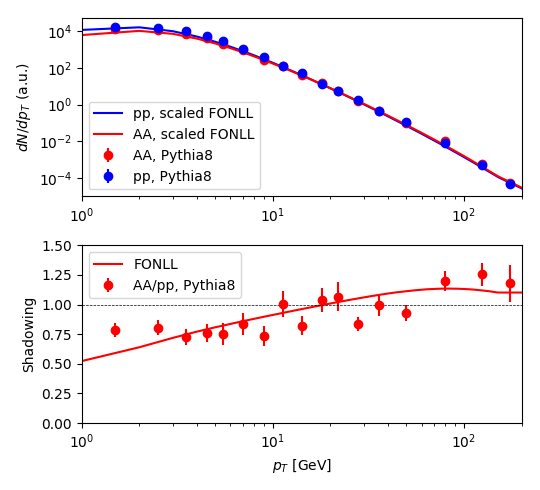
\includegraphics[width=.8\textwidth]{pythia-vs-fonll.png}
\caption{Top plot: a comparison of $D$-meson production in proton-proton collisions (blue) and in Pb-Pb collisions (red) with cold nuclear matter effect only. FONLL calculations are shown in lines and Pythia8 simulations are shown in symbols. Bottom plot: the ratio between the production in Pb-Pb collision (cold nuclear matter effect only) to the proton-proton baseline shows the nuclear shadowing effect.}
\label{fig:pythia-fonll}
\end{figure}

\section{Matching vacuum and medium-induced showers}
\subsection{A separate treatment of different phase-space}
\label{section:match}
The fate of vacuum-like showers in the hot-medium is complicated and there has not been a lot of phenomenological studies \cite{Cao:2017zih,PhysRevLett.120.232001,Caucal:2018tlu,Caucal:2018ofz}.
The prescription that we build in this section is by no means exact, but follow the reasoning from a recent work \cite{PhysRevLett.120.232001}.
The general idea is to identify different regions of phase-space of radiation, and apply different computation (DGLAP / transport) to different regions based on how much medium-modifications it would have received.

\begin{figure}
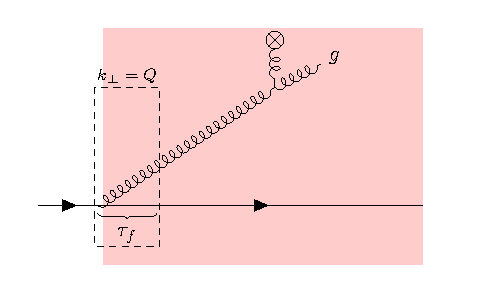
\includegraphics[width=.35\textwidth]{largeQ.pdf}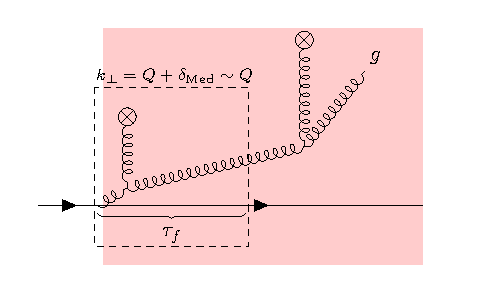
\includegraphics[width=.35\textwidth]{mediumQ.pdf}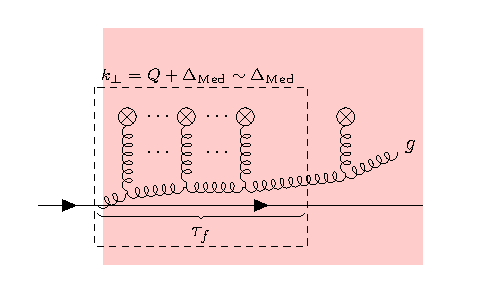
\includegraphics[width=.35\textwidth]{smallQ.pdf}
\caption{Demonstration of the medium corrections to vacuum-like radiation with different formation time. The energy of the gluon is hold fixed, while the virtuality is decreasing from left to right.}
\label{fig:vac-med-interface}
\end{figure}

Considering a vacuum splitting of a hard parton that enters the medium at $z=0$.
The vacuum splitting has formation time $\tau_f \sim 2x(1-x)E/k_\perp^2$.
It is very likely that the radiated gluon (or the quark) interacts with one or more scattering centers (labeled by ``i'') in the medium at time $t_i$.
Whether these interactions contribute coherently to the ``vacuum-like'' splitting follows the same argument as before.
Scatterings that are well separated from the formation processes $\tau_f \ll t_i$ are treated as independently, and it only broadens the transverse momentum without changing the probability of the process.
For $t_i \lesssim \tau_f$, the branching probability of the vacuum-like radiation also gets modified, in addition to broadening.
Now classifying the radiations using the average ``number'' of scatterings  $N = \tau_f/\lambda$ (for the case of a static medium),
\begin{itemize}
\item For a branching with large virtuality (left of figure \ref{fig:vac-med-interface}) so that $N \ll 1$ or equivalently $Q^2 \gg  g^2 x(1-x)E T$. 
The chance for the medium modification the vacuum branching probability is negligible. 
\item Hold the energy of the radiation and decrease its virtuality (middle of figure \ref{fig:vac-med-interface}) so that $N = \tau_f/\lambda \sim 1$ ($Q^2 \sim g^2 x(1-x)E T$). 
Now, there is an order one probability of scatterings within $\tau_f$, but the transverse momentum of the gluon is still dominated by the initial virtuality.
The probability for the branching should also be modified accordingly, for example, using the higher-twist formula that expanded in terms of $1/Q^2$.
\item Further decrease the initial virtuality of the branching (right of figure \ref{fig:vac-med-interface}) until $N = \gg 1$,
the medium broadening to the branching eventually dominates over the the virtuality.
And $Q^2 \sim g^2\sqrt{x(1-x)E T^3}$. 
When this happens, the branching probability is heavily modified by the medium and should be replaced by a medium-induced splitting calculation.
\end{itemize}
Summarizing the two extreme regions:
The DGLAP evolution is applied to the high-virtuality part of the shower $Q^2 \gg \alpha_s \omega T$ is not modified, while medium-induced calculations should be applied to the low-virtuality shower $Q^2 \sim \sqrt{\hat{q}\omega}$ (relation obtained in a static medium) via transport equations.
It is therefore natural to use the comparison relation between the partons's original virtuality $Q^2$ and the transverse momentum change contributed by medium broadening $\Delta k_\perp^2 = (\mathbf{k}_\perp(\tau=\tau_f) - \mathbf{k}_\perp(\tau=0))^2$ to separate the medium-induced radiation and the vacuum-like radiation.
The matching prescription is then to simply cut-out the vacuum branchings generated by Pythia in the region $\Delta k_\perp^2 \gtrsim Q^2$, the cut region is referred as the ``vetoed'' region in the literature \cite{PhysRevLett.120.232001}).
For a dynamical and fluctuating medium, there is no simple relation as $\Delta k_\perp^2\sim \sqrt{\hat{q}\omega}$ in the static medium, but the ``preformed parton'' technique can be used determined $\Delta k_\perp^2$ self-consistently for each vacuum branching (to be explained in the next paragraph).
Also in a finite medium, certain vacuum-like branchings may have a long formation time that it forms outside of the medium, from the uncertainty principle, these branchings do not resolve the details of the medium and its branching probability will not be modified in our model.
This separated treatment of different region of phase-space still depends on the detailed choice of the separation scale, so in the future, it would be ideal to develop a unified theoretical treatment for both vacuum and medium-induced shower in the time evolution picture.

Focusing only on the vacuum-like radiation generated by heavy quarks, one traces back a heavy quark line in the Pythia event recorder to find all the gluons from its final state radiation (FSR) and the original four momentum of the heavy quark at initial production vertex.
These FSR gluons are first treated as ``unformed'' by the transport models, and they are allowed to undergo elastic broadening with the medium.
In this way, by the time these gluons reaches its formation time ($t-t_0>\tau_f$), one knows both the initial virtuality and of the splitting $Q^2$, as well as how much medium broadening is acquired $\Delta k_\perp^2$.
Then, applying for our previous approximation, vacuum-like branching with 
$\Delta k_\perp^2 < R_v Q^2$ is unmodified, but $\Delta k_\perp^2 > R_v Q^2$ ones are rejected because this contribution is already taken care by the medium-induced rate in the transport model.
The order one $R_v$ parameter is introduced to parametrize the uncertainty in this matching scale.

\subsection{Visualizing the matching on the Lund diagram}
The Lund diagram is a useful tool to visualize the phase-space for high energy parton splitting.
There are many different choice of kinematic variables, but here we choose the vertical axis to be $Y = \ln(1/x) = \ln(E/\omega)$, and the horizontal 
axis to be $X = ln(1/\theta^2) = \ln(\omega^2/k_\perp^2)$.
Here $x$ is the energy fraction carried by the daughter paron in a particular splitting, and $\theta$ is the daughter's emission angle relative to the mother parton.
This arrangement is inspired by the soft and collinear limit of the QCD splitting function (for example $q\rightarrow q+g$),
\begin{eqnarray}
dP^{q}_{qg} \sim \frac{\alpha_s C_F}{\pi} \frac{dx}{x}\frac{d\theta^2}{\theta^2} = \frac{\alpha_s C_F}{\pi} d\ln\frac{1}{x} d\ln\frac{1}{\theta^2}.
\end{eqnarray}
Therefore, the probability distribution of a vacuum-like splitting vertex should be uniform, apart from the running coupling effect.
The closer a point lies towards the origin, the higher its virtuality.
The soft and collinear radiations reside at large $X$ and $Y$.
Also, constant-formation-time contours are simply straight lines $Y+X=\ln(E\tau_f/2)$.

On the left of figure \ref{fig:lund}, we show the phase space occupied by the vacuum branching without medium (left); on the right, it is medium-modified vacuum splitting (blue color map) and the medium induced radiation (red contour) from our simulation.
The simulation first finds out charm quark with transverse momentum $90 < p_T <110$ GeV at the production vertex in Pythia, and then propagate it and its vacuum radiated gluons in a static medium with $T=0.3$ GeV with $\alpha_s = 0.3$ for a path length $L$.
We see that without the medium effect, the vacuum radiations fills the region bounded by time-evolution limit $\tau_f < L$ (dash-dotted line) and the default non-perturbative bounds $k_\perp > 0.4$ GeV (dotted line) of Pythia. 
Inside the medium, the medium-induced radiations distributed around the line $\tau_f\hat{q} = k_\perp^2$ which is $\theta^4\omega^3 = 2\hat{q}$ (dashed line) in the soft limit.  
But this line is only an averaged estimation of the relation between $k_\perp, \omega$ and $\hat{q}$, the actually outcome of the simulation has huge fluctuation.
The triangle area bounded by the line $\tau_f < L$ and the line $\theta^4\omega^3 = 2\hat{q}$ is where the vacuum-like radiation receives large modification from medium interactions.
The rejection program introduced before suppress the vacuum-like radiation in this region compared to the case without a medium.
Again, due to fluctuations, the triangle region is not an entirely vetoed as the one demonsrated in \cite{PhysRevLett.120.232001}.

\begin{figure}
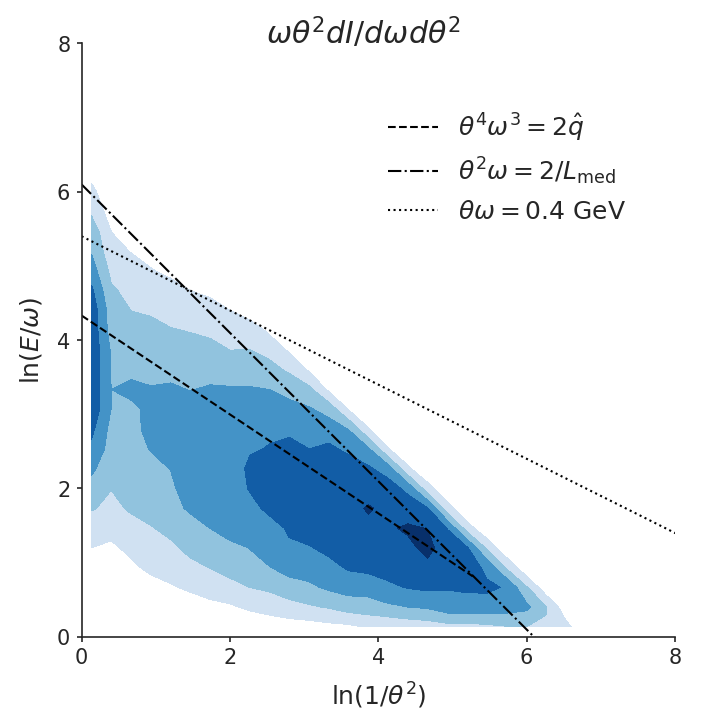
\includegraphics[width=.5\textwidth]{lund-vac.png}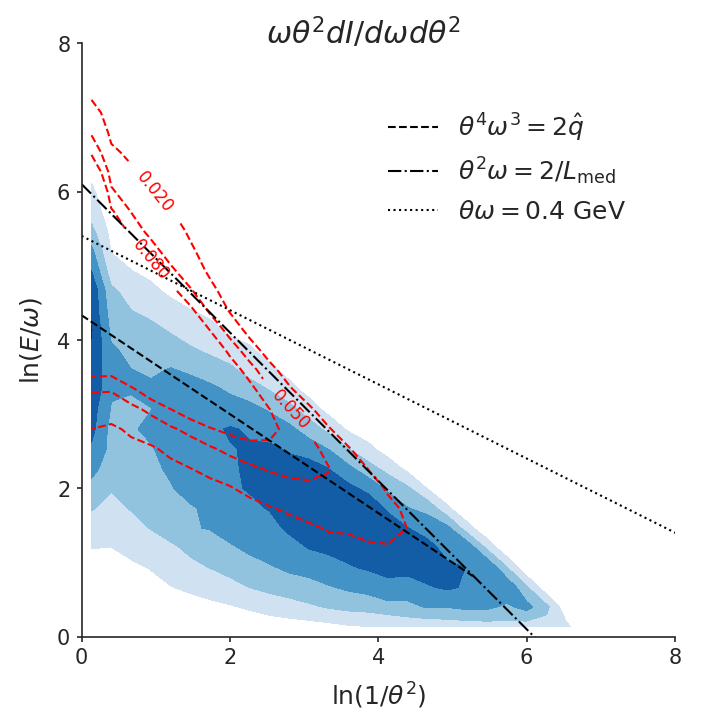
\includegraphics[width=.5\textwidth]{lund-med.png}
\caption{Plotting the gluon radiations from a charm quark on the Lund diagram. The gluon emission has an energy $\omega$ with angle $\theta$ with respect to the heavy quark. The blue heat map in the left plot shows the distribution of vacuum-like emissions without medium effects. The heat map in right left plot shows the distribution of vacuum-like emissions with medium effects; while the red contour stands for the medium induced emissions. Emissions on the black dashed lines have $k_\perp^2 = \sqrt{2\omega \hat{q}}$. Emissions on the dashed-dotted lines have a formation time equals to the medium path-length. Finally, the dotted lines is the non-perturbative cut-off in Pythia $k_\perp = 0.4$ GeV.}
\label{fig:lund}
\end{figure}

Concluding this section, the realm of the transport equation and the DGLAP evolution is separated when the parton virtuality is comparable to the acquired transverse momentum broadening within the formation time.
High virtuality evolution is approximated as unmodified, while low virtuality evolution is terminated and replaced by the medium-induce processes via the transport evolution. 
Using the Lund diagram to visualize the simulation, medium-induced and vacuum branchings occupy relatively separated region of the phase-space, though smeared by a large fluctuation.
This procedure is, of course, only viable if we initialize the simulation with parton shower event generator.
We are not able to do such a separation using heavy quark spectra obtained from FONLL.

\section{Particles coupled to an evolving medium}
\label{section:couple-to-hydro}
The coupling between hydrodynamics and hard parton transport often require a switching of different reference frames, as velocity of the medium local-rest-frame relative to the lab frame is function of space-time.

\paragraph{For diffusion dynamics} The diffusion equations are most easily  written in the local-rest-frame of the medium.
Given a particle's four momentum in the lab frame ($p_{L}^\mu$), one first boost it into the medium local-rest-frame ($p_{M}^\mu$),
\begin{eqnarray}
p_{M}^\mu &=& L^\mu_\nu(\vec{\beta}) p_{L}^\nu\\
L^\mu_\nu &=& 
\begin{bmatrix}
\gamma & -\gamma\vec{\beta}\\
-\gamma\vec{\beta} & \mathbb{1} + \frac{\gamma^2}{\gamma+1}\vec{\beta}\vec{\beta}
\end{bmatrix}
\end{eqnarray}
where $\vec{\beta}$ is the velocity of the fluid cell relative to the lab frame, and $L^\mu_\nu$ is the Lorentz transformation.
One needs to be careful with that the time step in the fluid rest frame $\Delta t_{M}$ is different from the one in the lab frame $\Delta t_{L}$.
Consider the particle trajectory $\Delta x_{L}^\mu$ within $\Delta t_{L}$ observed in the lab frame and boost it into the medium frame,
\begin{eqnarray}
\Delta x_{L}^\mu = \frac{p_{L}^\mu}{E_L} \Delta t_{L} \xrightarrow{\textrm{boost}} \Delta x_{M}^\mu = \frac{L^\mu_\nu(\mathbf{v}_{M}) p_{L}^\nu}{E_L} \Delta t_L = \frac{p_{M}^\mu}{E_L} \Delta t_L
\end{eqnarray}
Now compare the time-component of the equation, one get the time step in the medium frame is related to the lab frame step by the ratio between the energy of the particle in the two reference frames,
\begin{eqnarray}
\Delta t_M = \frac{E_M}{E_L} \Delta t_L
\end{eqnarray}
Once the momentum is updated in the medium frame to become $p'_M$, it is boosted back to the lab frame,
\begin{eqnarray}
x'^{\mu} &=& x^{\mu} + \frac{p_{L}^\mu}{E_L} \Delta t_{L} \\
p_{L}^{'\mu} &=& L^\mu_\nu(-\vec{\beta}) p_{M}^{'\nu}
\end{eqnarray}
where we have chosen to update position before the update of the momentum.

The choice of $\Delta t_L$ is also tricky. 
A most straightforward uniform time step for all the particles is not the optimal choice.
This is because that relativistic hydrodynamics for heavy-ion collision is often solved in the $(\tau,x,y,\eta_s)$ coordinates, and the hydrodynamic field is propagated from one constant proper time $\tau = \sqrt{t^2 - z^2}$ to the next.
There are two consequences if we choose the same $\Delta t_L$ for all particles:
\begin{itemize}
\item[1.] Different particles will be at different proper times $\tau$ at a constant $t$. It requires the program to load the entire hydrodynamic temperature and velocity history into the memory, which can be a potential problem for 3+1 D hydro simulation (the memory consumption for boost-invariant hydrodynamics is not critical).
\item[2.] The time step in medium-rest-frame for particles at large space-time rapidity would be too small.
\end{itemize}
For these practical reasons, we choose to propagate particles with a constant proper-time step $\Delta \tau$. 
As a result, the time step in the lab frame is different for each particle, depending on its location and momentum, and is solved by,
\begin{eqnarray}
\Delta \tau = \sqrt{(t+\Delta t_L)^2 - (z+v_z \Delta t_L)^2} - \sqrt{t^2 - z^2}.
\end{eqnarray}
This is (keeping the positive solution),
\begin{eqnarray}
\Delta t_L(p, x) = \frac{-(t-z v_z) + \sqrt{(t-z v_z)^2 - (1-v_z^2)(\Delta \tau^2 + 2\sqrt{t^2 - z^2}\Delta \tau )}}{2(1-v_z^2)}
\label{eq:dt-transformation}
\end{eqnarray}
This adaptive time step propagate a particle between constant proper-time hyper-surface, therefore only two steps of hydrodynamic information needs to be loaded into memory at a time.
Also $\Delta t_L$ becomes larger for forward/backward particles.

\paragraph{For matrix-element scattering} The situation for matrix-element scatterings is more complicated.
Because the initial state of scattering is straightforwardly sampled in the medium local-rest-frame, but the full final state is most efficiently sampled in the center-of-mass frame of the few-body collisions.
The center-of-mass velocity relative to the local-rest-frame is,
\begin{eqnarray}
\vec{\beta}_{C} = \frac{\sum_{i\in \textrm{IS}} \vec{p}_i}{\sum_{i\in \textrm{IS}} E_i}
\end{eqnarray}
where ``IS'' stands for the initial state.

\begin{itemize}
\item[1.] For each hard parton, determine $\Delta t_L$ with equation \ref{eq:dt-transformation}.
\item[2.] Boost the particle to the medium rest-frame and sample the scattering rate $\Delta t_M R$ channel, and then sample the medium parton(s) that forms the scattering initial state with the hard parton.
\item[3.] In the CoM frame of the initial state, sample the final state particles.
\item[4.] Boost back the final state particles to the medium rest frame.
\item[5.] Boost back to the lab frame.
\end{itemize}

\section{Heavy-flavor hadronization and hadronic stage}
\label{section:hadronization}
At a temperature around $T_c$, light hadrons can be sampled from the hydrodynamics energy momentum tensor statistically.
For hard partons that stay more off equilibrium, a more microscopic hadronization model is in need.
The final hadronic system is also dense enough for the heavy hadron to interact.
Though the hadronic interactions are not analyzed so extensively as the QGP interaction, studies have shown hadronic rescatterings contributes finte low-$p_T$ $v_2$ of D-meson \cite{Cao:2015hia}.
Therefore we also includes the afterburner stage for the heavy flavors.

\subsection{The ``sudden" approximation of hadronization} 
The hadronization implementation is described in \cite{Cao:2013ita}.
It combines the fragmentation of heavy quark at high momentum and the recombination with medium partons into hadrons at low momentum.
The hadronization is treated to be instantaneous on an isothermal hypersurface.
This ``sudden'' approximation certainly has certain drawbacks.
First, hadronization is a long distance process. 
In the rest frame of the heavy flavor, it takes time scale $1/\Lambda_{QCD}$. 
With a large boost factor $E/M_{\textrm{hadron}}\sim E/M_{\textrm{heavy quark}}$, the formation time of the heavy hadron can be comparable to macroscopic length scales.
For example, for a moderate $E=10$ GeV charm quark $M=1.3$ GeV, this time is estimated to be $8$ fm/c, which is certainly not a sudden process considering the hydrodynamic stage only last for $O(10)$ fm/$c$.
Second, an instantaneous recombination process breaks energy conservation and detailed balance.
Toward a solution to all these problems, one may need to consider using a dynamical hadronization model \cite{He:2019vgs}.

\paragraph{Fragmentation} 
In high energy electron-positron collision and proton-proton collision, high momentum heavy quark hadronizes through the fragmentation mechanism.
The energetic heavy quark produces a bunch of hadrons with a heavy hadron that carries a certainty fraction of the origin quark energy $z = p_H/p_Q$.
The probability distribution of $z$ is known as the fragmentation function $D(z)$, and can be measured in, e.g., electron-positron collier.
There are different parametrizations for $D(z)$ and the Peterson fragmentation function \cite{PhysRevD.27.105} used in the present study,
\begin{eqnarray}
D(z) \propto \frac{1}{z(1-\frac{1}{z} - \frac{\epsilon}{1-z})^2}
\end{eqnarray}
where $\epsilon$ is a parameter that scales as $m_Q^{-2}$ ($\epsilon_c \approx 0.05, \epsilon_b \approx 0.006$).

\paragraph{Recombination}
It was known already in proton-proton collision that heavy quark can hadronize into mesons by the recombination with a light quark in the proton remnant \cite{Mehen:2003rf}.
In a heavy-ion collision, recombination mechanism can play an important row for low transverse momentum heavy flavors, given the abundance of the medium thermal partons.
Early study in the nuclear collisions \cite{Oh:2009zj} assumes that the recombination probability can be computed from the wave function overlap between initial state partons and final state mesons or baryons, with the momentum of the medium parton integrated over the thermal distribution.
\begin{eqnarray}
\frac{dP_M(p', p)}{dp'^3} &=& \int dk^3 n_{\bar{q}}(k) W_{M}(p, k)\delta^{(3)}(\vec{p}'-\vec{p}-\vec{k}), \label{eq:meson_recombine}\\
\frac{dP_B(p', p)}{dp'^3} &=& \int dk_1^3 dk_2^3 n_{\bar{q}}(k_1)  n_{\bar{q}}(k_2) W_{B}(p, k_1, k_2)\delta^{(3)}(\vec{p}'-\vec{p}-\vec{k}_1 - \vec{k}_2), \label{eq:baryon_recombine}.
\end{eqnarray}
On the left are the differential probability for a heavy quark with momentum $p$ to hadronize into a heavy meson (first line) or a heavy baryon (second line) with momentum $p'$ through recombination.
They are equal to an integration of light quark(s) / anti-quark momentum  of the production of baryon /meson Wigner function $W$ times the thermal distriubtion function, subjected to three-momentum conservation.
It is evident that the energy conservation is not imposed in the instantaneous $2\rightarrow 1$ coalescence approach.
The quark / anti-quark distribution function is the Fermi-Dirac one, neglecting chemical potential, 
\begin{eqnarray}
n = \frac{g_q V}{e^{\beta p\cdot u} + 1}
\end{eqnarray}
with $u$ the fluid velocity and the $p$ the four momentum of the light quark / anti-quark.
$g$ is the degeneracy of the quark, and $V$ is a test volume that will eventually be canceled by the normalization factor in the the Wigner function.
As a remark, we have assumed in the transport model that medium partons are massless because the thermal masses are higher effects for energy loss; but for recombination into bound states near $T_c$, it is important to use non-perturbative constituent masses of light quarks $m_u = m_d = 300$ MeV and $m_s = 475$ MeV.

Regarding the meson wave-function, there has been efforts using Dirac equation and to obtain a more realistic wave-function for different state of heavy mesons.
But the current model uses parametrized Gaussian wave-function for simplicity,
\begin{eqnarray}
\phi_M(\vec{r}) &=& \left(\frac{1}{\pi \sigma^2}\right)^{3/4} e^{-\frac{r^2}{2\sigma^2}}
\end{eqnarray}
The $\sigma$s are related to the reduced mass of the two body system $\mu = m_1 m_2/(m_1+m_2)$ and the frequencty of the  two-body potential $\omega$ by $\sigma = 1/\sqrt{\mu \omega}$.
These frequencies is estimated from the charge radius of different heavy mesons: $0.106$ GeV for charmed hadron and $0.059$ GeV for the bottom mesons.
The Wigner function is defined in terms of the relative distance $\vec{r}$ and relative momentum $\vec{q}$ between the quark and anti-quark,
\begin{eqnarray}
W_M(\vec{r}, q^2) &=& g_M \int d^3 \vec{a} e^{-i\vec{q}\cdot \vec{a}} \phi_M(\vec{r}+\vec{a}/2) \phi_M^*(\vec{r}-\vec{a}/2) \\
\vec{q} &=& \frac{E_2\vec{p}_1 - E_1\vec{p}_2}{E_1+E_2}.
\end{eqnarray} 
Averaging over the light quark's positions,
\begin{eqnarray}
W_M(q^2) &=& \frac{g_M}{V} (2\sqrt{\pi}\sigma)^3 e^{-\sigma^2 q^2},
\end{eqnarray}
which is the quantity needed in equation \ref{eq:meson_recombine},
\begin{eqnarray}
\frac{dP_M(p',p)}{dp'^3} &=& \int dk^3 \frac{g_q g_M}{e^{\beta p\cdot u} + 1} (2\sqrt{\pi}\sigma)^3 e^{-\sigma^2 q^2} \delta^{(3)}(\vec{p}'-\vec{p}-\vec{k}),
\end{eqnarray}
where the test volume in the distribution function has been canceled by the one in the Wigner function.

The same procedure applies to heavy baryon, with the three-body Wigner function in the Gaussian approximation as,
\begin{eqnarray}
f_B^W(q_1^2, q_2^2) = \frac{N g_B}{V^2} (2\sqrt{\pi\sigma_{1,2}\sigma_{12,3}})^6 e^{-q_{1,2}^2 \sigma_{1,2}^2 - q_{12,3}^2 \sigma_{12,3}^2}.
\end{eqnarray}
With the relative momenta defined as,
\begin{eqnarray}
\vec{q}_{1,2} &=& \frac{E_2 \vec{p}_1 -E_1\vec{p}_2}{E_1+E_2}\\
\vec{q}_{12,3} &=& \frac{E_3 (\vec{p}_1+\vec{p}_1) - (E_1+E_2)\vec{p}_3}{E_1+E_2 + E_3}
\end{eqnarray}
And the $\sigma$ related to the frequency and masses by,
\begin{eqnarray}
\sigma_{1,2}^{-1} &=& \sqrt{\omega \frac{m_1m_2}{m_1+m_2}}\\
\sigma_{12,3}^{-1} &=& \sqrt{\omega \frac{(m_1+m_2)m_3}{m_1+m_2+m_3}}
\end{eqnarray}

To synthesis these two competing mechanisms of hadronization, one first samples the recombination probability in equations \ref{eq:meson_recombine} and \ref{eq:baryon_recombine} and determines whether the heavy quark coalesces with the medium partons. 
If not, its hadronization will be handled by the Pythia fragmentation routine with the Peterson fragmentation function.

\subsection{Hadronic rescattering}
Currently, the hadronic rescattering of charmed mesons with $\pi$ and $\rho$ mesons are included the UrQMD frame as the light hadrons. 
These cross-sections are obtained from \cite{Lin:2000jp}.
Hadronic cross-section of the charmed baryons and bottom hadrons are not included.

One modification is made to the UrQMD heavy-flavor sector that the back reaction from heavy flavor mesons to light sector is turned-off. 
This is done by resetting the light scattering partner's four momentum back to its initial value.
This is to the same level of approximation of the linearized transport equation in the QGP phase, and allows for an easy oversampling of the number of heavy flavor particles to obtain better statistics.

\section{Benchmark calculation of observables}
\label{section:benchmark}
In the last section of this chapter, we provide a benchmark calculation of this open-heavy flavor simulation framework to experimental data, systematic calibration of model parameters and uncertainties will be discussed in the next two chapters.

\subsection{Open heavy flavor observables}
Experimentally, the ground states mesons $D^0, \bar{D}^0, D^{\pm}, B^{\pm}, D_s^{\pm}, B_s^{\pm}$ and the excited states $D^{*\pm}$ can be measured in the experiments. 
Their nuclear modification factor, momentum anisotropy has been measured at both LHC and RHIC.
Currently, we focus on comparing to non-strange D and B mesons data.
Though strange heavy meson $D_s, B_s$ are also very interested as they contain the strangeness enhancement information, but the strangeness physics is not the main focus of this work.

The nuclear modification factor has already been introduced in the chapter \ref{chapter:introduction}. 
Here we summarize how the momentum anisotropy observables of are computed.
A list of the measurements and references can be find in table \ref{table:ALICE-obs} and table \ref{table:CMS-obs}.
\begin{center}
\begin{table}[h]
\caption{ALICE dataset}\label{table:ALICE-obs} 
\begin{tabularx}{\columnwidth}{XXX}
\hline 
 Observables & Centrality & Reference\\ 
\hline 
$D$-meson $v_2$ & 30-50\% & {Acharya:2017qps}\\ 
\hline 
Event-engineered $D$-meson $v_2$ & 30-50\% & {Grosa:2017zcz}\\ 
\hline 
$D$-meson $R_{AA}$ & 0-10, 30-50, 50-80\% & {Acharya:2018hre}\\
\hline 
\end{tabularx}
\end{table}
\begin{table}[h]
\caption{CMS dataset}\label{table:CMS-obs} 
\begin{tabularx}{\columnwidth}{XXX}
\hline 
Observables & Centrality & Reference\\ 
\hline 
D${}^0$-meson $v_2$ & 0-10, 10-30, 30-50\% & {Sirunyan:2017plt}\\ 
\hline 
D${}^0$-meson $R_{AA}$ & 0-10\%, 0-100\% & {Sirunyan:2017xss}\\ 
\hline 
B${}^{\pm}$-meson $R_{AA}$ & 0-100\% & {Sirunyan:2017oug}\\ 
\hline 
\end{tabularx}
\end{table}
\end{center}

\paragraph{Momentum anisotropy}
Heavy flavors momentum anisotropy at high-$p_T$ is thought to be the result of aisntorpic energy loss, because hard partons emitted in the short axis direction losses less energy than those emitted from the long axis direction on average.
At low momentum, the momentum anisotropy has a flow origin that heavy quark interacts so frequently with the medium and tends to catch up with the flow velocity of the medium.
Both mechanisms produce $v_2$ relatively the common reference of bulk geometry / bulk flow.
The $p_T$ differential $v_2$ is usually measured in two-particle correlation approach,
\begin{eqnarray}
v_n\{2\}(p_T) = \frac{\mathfrak{Re}\langle d_n\{2\} \rangle}{\langle c_n\{2\}\rangle}.
\end{eqnarray}
$c_n$ is the event-wise two particle correlation of $N$ reference particles (REF, the bulk medium) within a certain kinematic range,
\begin{eqnarray}
c_n &=& \frac{|Q_n|^2 - N}{N(N-1)},  \\
Q_n &=& \sum_{i=1}^N e^{i n \phi},
\end{eqnarray}
and the event average ($\langle\cdots\rangle$) is weighted by $N(N-1)$.
$d_n$ is the correlation between the $M$ particles of interest (POI, in this case the heavy flavors) and the $N$ reference particles,
\begin{eqnarray}
d_n &=& \frac{q_n Q_n^* - m}{MN-m},  \\
q_n &=& \sum_{j=1}^M e^{i n \phi}
\end{eqnarray}
$m$ is the number of POI that is also counted as REF to subtract auto-correlations. 
The event average is weighted by the number of pairs $MN-m$.

\paragraph{Event-shape engineering on heavy-flavor $v_2$}
Event-shape engineering is a more recent idea to look at the detailed response of the hard sector to the medium geometry.
Experimentally, an ensemble of events belongs to a certain centrality class is further classified according to its ``event shape'', measured by $q_2$,
\begin{eqnarray}
q_2 = \frac{|Q_2|}{\sqrt{N}}.
\end{eqnarray}
Due to event-by-event geometry fluctuation, the event shape in the a given centrality class can be vary dramatically.
The ALICE experiment then measures the D meson $v_2$ with events having the $20\%$ largest $q_2$ and events with the $60\%$ smallest $q_2$.
They found a large separation between the the resulting $v_2$ with biased selected events compared to the $v_2$ calculated from unbiased events.
This measurement quantifies the response of hard probe to the event geometry fluctuation while controlling multiplicity. 

\subsection{A first comparison to data}
We do not intend optimize all the parameters in the model in this first comparison to data, but uses reasonable guess of the parameters to understand the model.
The TRENTo parameters and the hydrodynamic transport coefficients are obtained from the high likelihood parameters in \cite{Bernhard:2018hnz}.
The heavy quark flavor starts to lose energy from $0.6$ fm/$c$, and the matching condition between the vacuum-like radiation and the medium-induced radiation is $\Delta k_\perp^2 = R_v Q^2$ with $R_v = 1$.
We used only leading order contribution from the weakly coupled theory, and tried both fixed coupling and running coupling.
The default switching scale between a large-$Q$ scattering small-$Q$ is $Q_{\textrm{cut}}^2 = 4 m_D^2$.

\begin{figure}
\centering
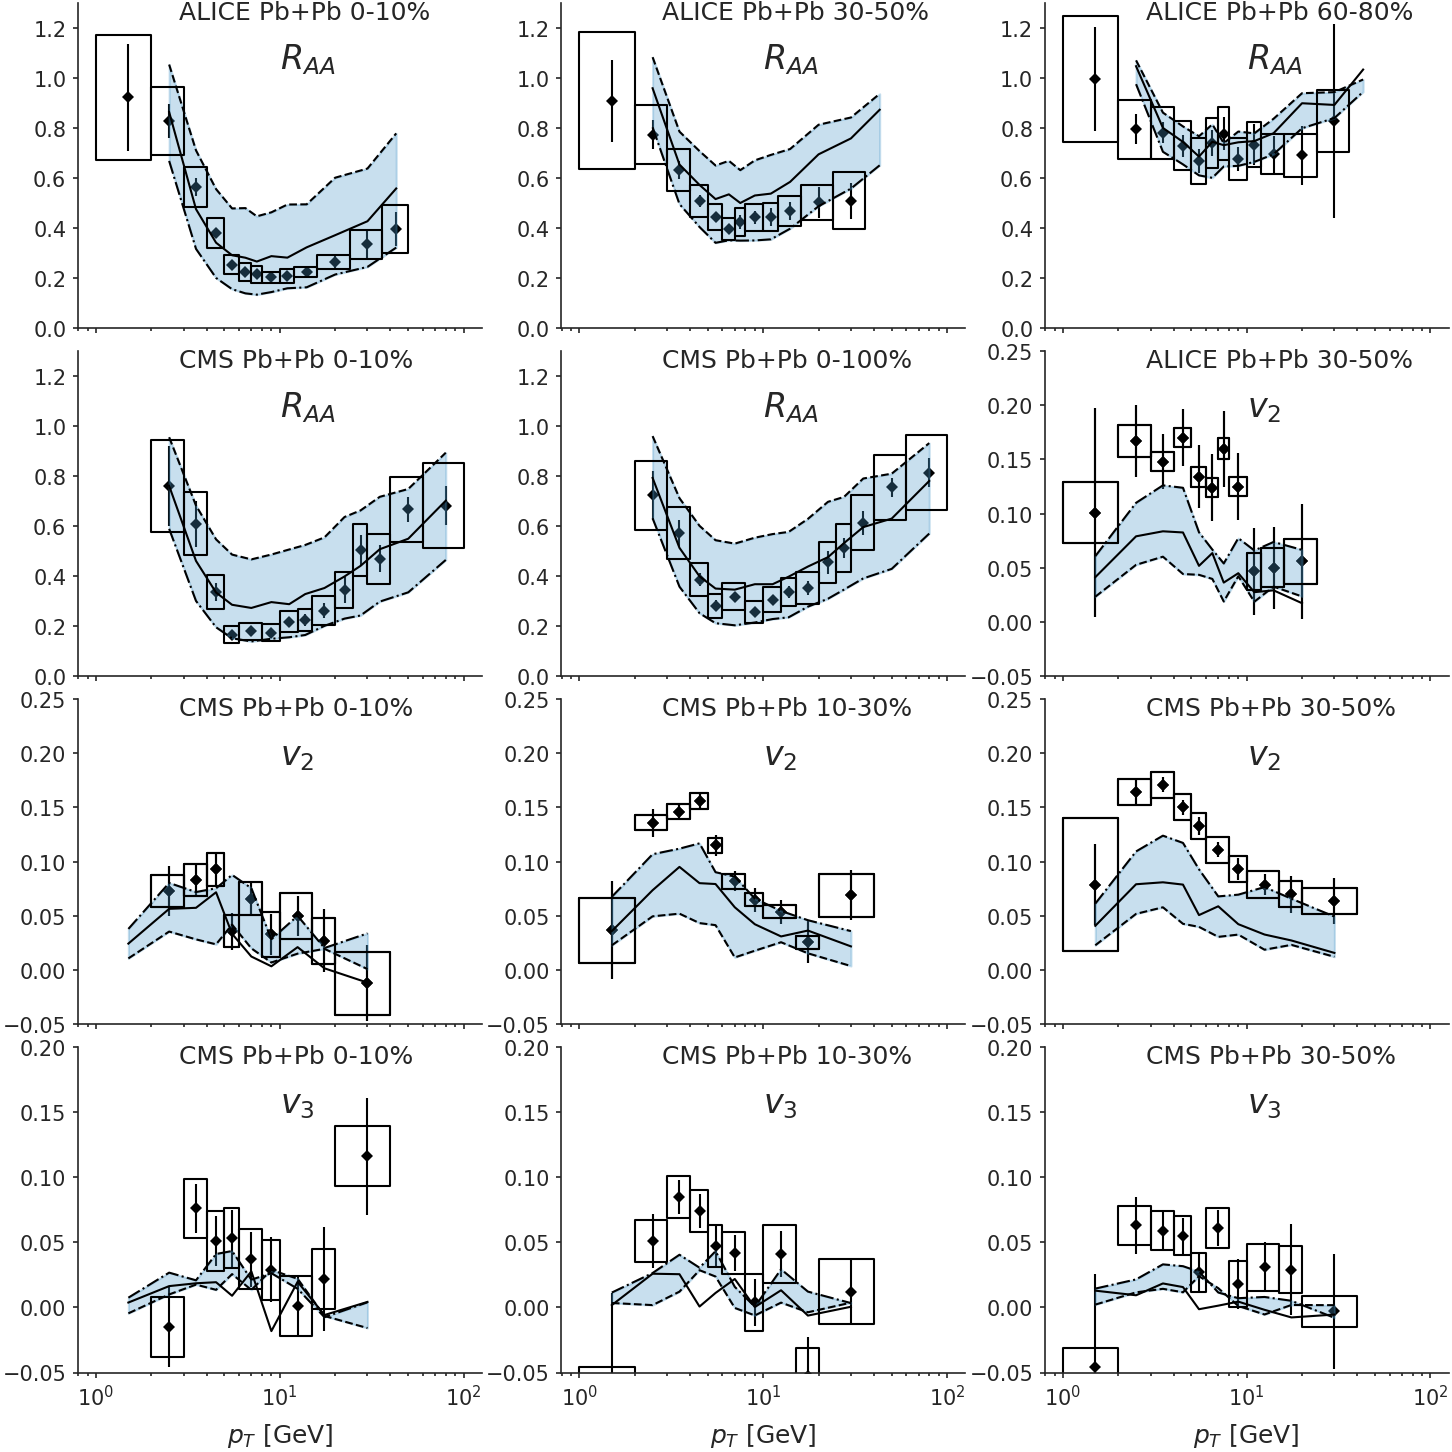
\includegraphics[width=\textwidth]{fix_alphas.png}
\caption{Benchmark results using fixed coupling constant $\alpha_s = 0.2$ (dashed), $0.3$ (solid), and $0.4$ (dash-dotted). The blue bands fill between the results using $\alpha_s=0.2$ and $0.4$. They are compared to the experimental data (black symbols) obtained by the ALICE Collaboration \cite{Acharya:2017qps,Acharya:2018hre} and the CMS Collaboration \cite{Sirunyan:2017xss,Sirunyan:2017plt}.}
\label{fig:new:fix-a}
\end{figure}

\paragraph{Fixed coupling} First, we compute with fixed coupling constant.
It should be understood as an effective in-medium coupling for both elastic and radiative processes.
In figure \ref{fig:new:fix-a}, we present the results (lines and bands) with data points measured at $\sqrts{s} = 5.02$ TeV for D mesons (symbol with errorbars and boxes).
Different line shapes corresponds to different coupling $\alpha=0.2$ (dashed), $0.3$ (solid), and $0.4$ (dash-dotted). 
The types of observables are shown within each subplots, indicating the experiment collaboration, the collision system and the centrality.

Looking at the experimental measurements, $R_{AA}$ increases with the centrality classes and displays a minimum around $8 < p_T < 10$ GeV.
In the high-$p_T$ end, the $R_{AA}$ increases towards the baseline around one. 
This increase is slow, noticing the $p_T$ is plotted on a log scale.
In the low-$p_T$ end, the $R_{AA}$ quickly rises.
There are many reasons for this, for example, the feeding from higher-$p_T$ particles due to energy loss;  the feeding from low-$p_T$ particles that are pushed outward by the strong medium radial flow.
In addition, the recombination hadronization mechanism also plays a part, as the D meson is gaining momentum (on average) in the recombination process.
Based on the comparison to $R_{AA}$, a phenomenological value for a fixed $\alpha_s$ is around $0.3$--$0.4$.
However, such values cannot explain the large momentum anisotropy in mid-central collisions, e.g. centrality 30-50\%.
This is known as the $D$ meson $R_{AA}$--$v_2$ puzzle, which also appears for leading light hadrons.
There has been different solutions to this problem, such as the proposed sudden increase of the interaction strength near $T_c$, fine tuning the general temperature-momentum dependence of the transport coefficients, etc \cite{SCARDINA2016329,Xu:2017obm,Shi:2018vys}.
In the next two chapters, we will see if this discrepancy can be compensated by a fine tuning of parameters in the current model.
A non-zero $v_3$ of $D$ meson is an evidence of heavy-flavor coupling to the detailed event-by-event nuclear geometry fluctuation.
The calculation of $v_3$ is systematically below the data, despite the large statistical and systematic uncertainty,

\begin{figure}
\centering
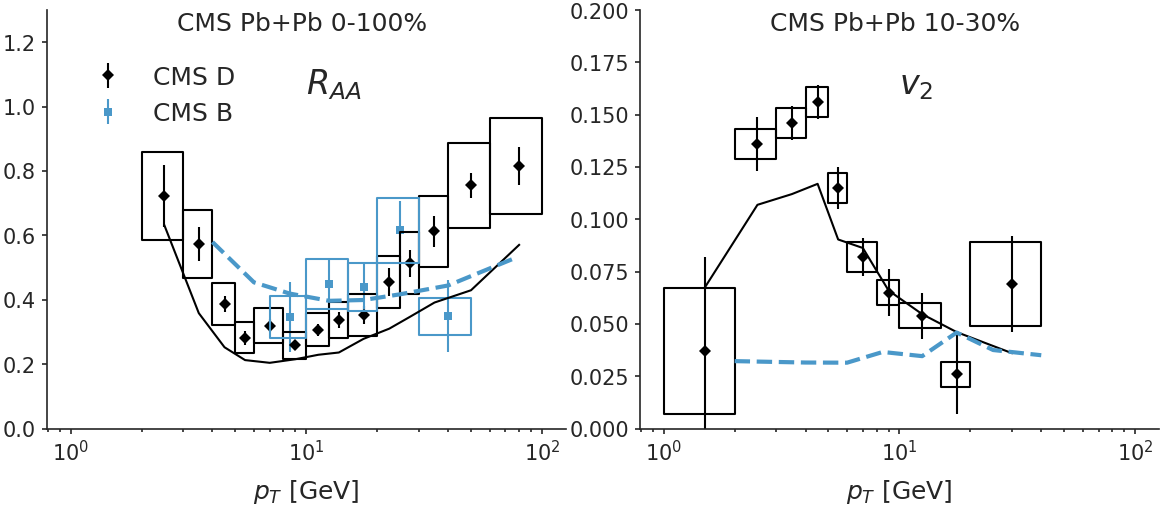
\includegraphics[width=\textwidth]{run_alphas_DB.png}
\caption{Demonstrating the mass dependence of the observables using $\alpha_s = 0.4$. 
The D meson and B meson results are labeled by color black and blue respectively.
Left plot: $R_{AA}$ for 0-100\% centrality. Right plot: $v_2$ for 10-30\% centrality.}
\label{fig:new:fix-DB}
\end{figure}

In figure \ref{fig:new:charm-bottom}, we compared the calculation with $\alpha_s = 0.4$ for charmed meson $R_{AA}^D$ and bottom meson $R_{AA}^B$ at $0-100\%$ centrality and D meson and B meson flow at $10-30\%$ centrality.
The mass effect of bottom quark is much stronger than charm quark, therefore, $R_{AA}^B$ at intermediate $p_T$ is higher than $R_{AA}^D$. 
At very high $p_T$, the ``Dead-Cone'' of bottom quark also becomes insignificant, and the B and D meson $R_{AA}$ converge.
Unlike the sudden increase of $v_2^D$ at low $p_T$, $v_2^B$ is always small, meaning that the bottom quark does not catch up the medium flow as the charm does and remains far from equilibrium.

\begin{figure}
\centering
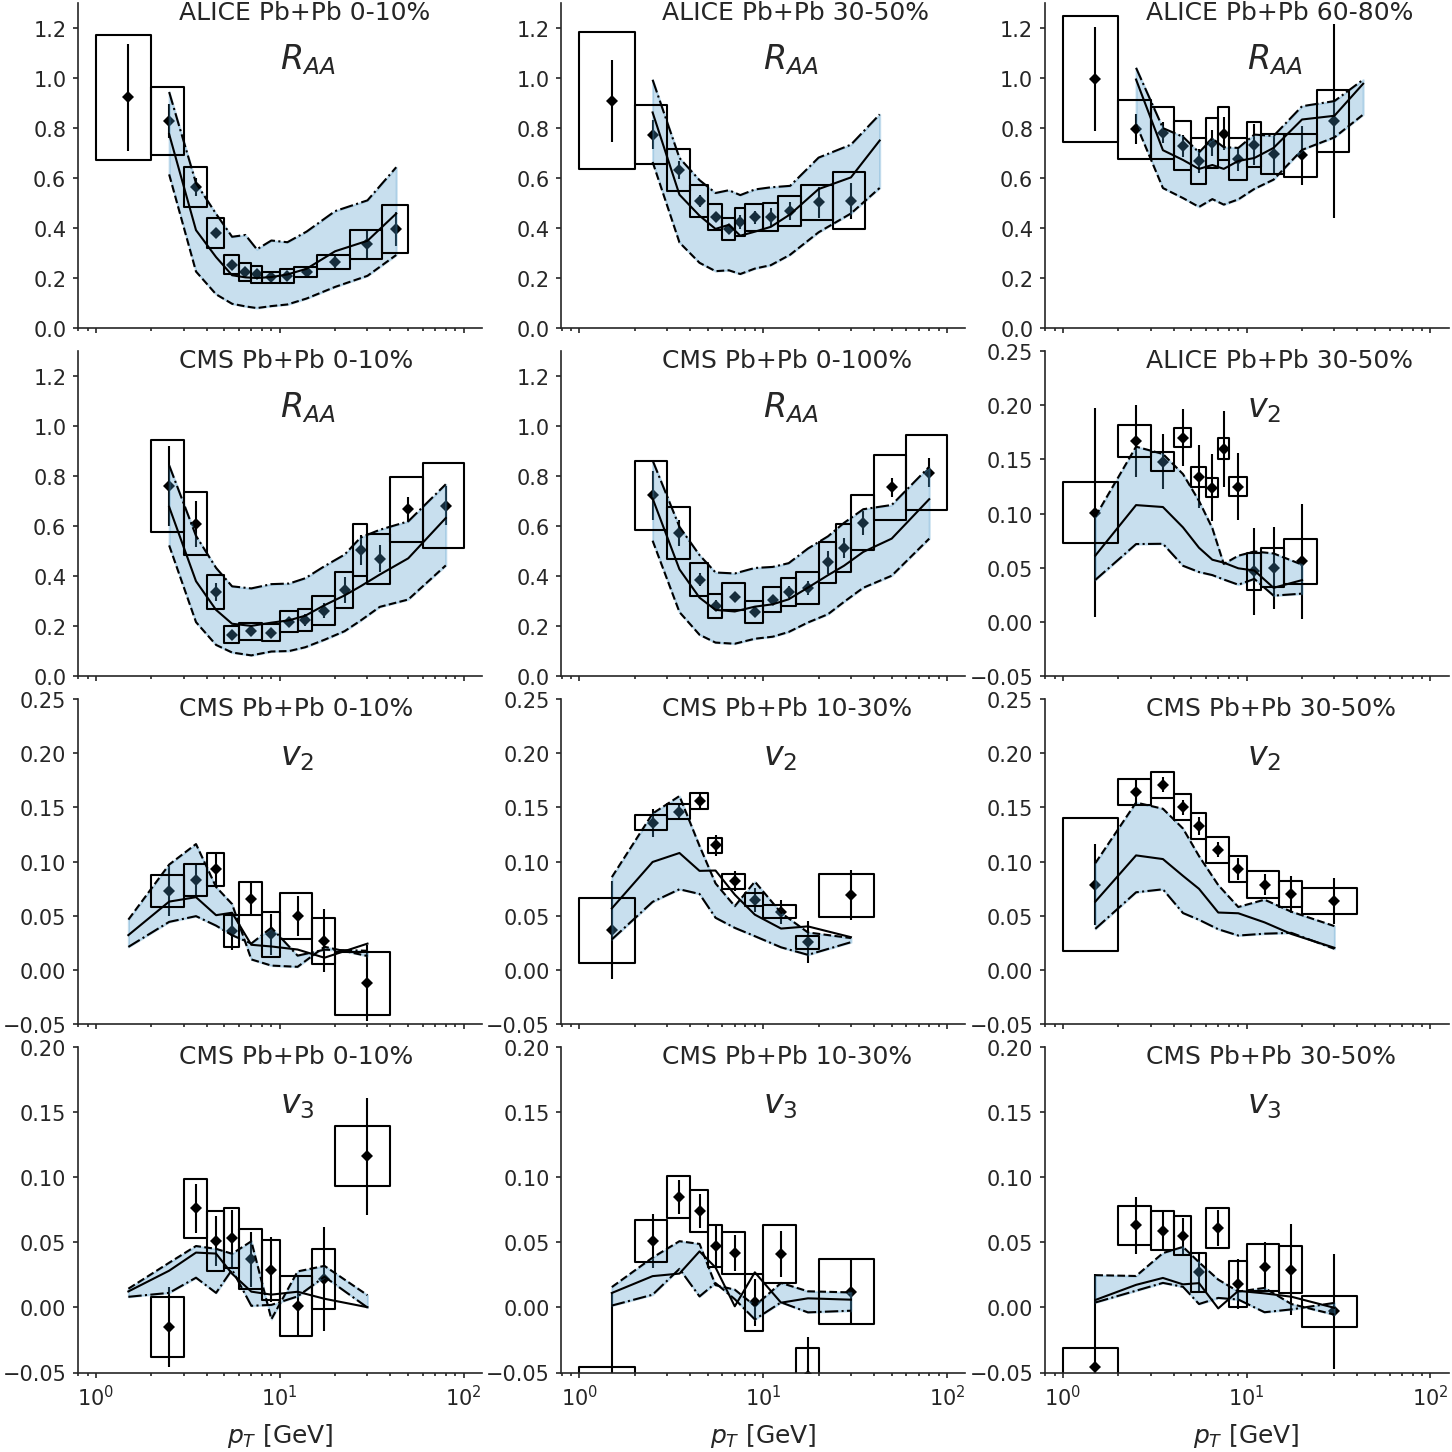
\includegraphics[width=\textwidth]{run_alphas.png}
\caption{Benchmark results using running coupling constant. The medium scale that stops the low-$Q$ running is chosen at $Q_{\textrm{med}} = \mu\pi T = \pi T$ (dashed), $2\pi T$ (solid), and $4\pi T$ (dash-dotted). They are compared to the experimental data (black symbols) obtained by the ALICE Collaboration and the CMS Collaboration.}
\label{fig:new:run-a}
\end{figure}

\paragraph{Running coupling} Moving to a running coupling constant, the uncertainty of the in-medium coupling strength is transferred to the uncertainty of the medium scale in the running $\alpha_s$,
\begin{eqnarray}
\alpha_s(Q) = \frac{2\pi}{9}\frac{1}{\ln \left( \max\{Q, \mu\pi T\} / \Lambda\right)}.
\end{eqnarray}
Due to the running, heavy quark radiation at high energy will be reduced compared to low energy and the interaction strength with the medium is enhanced at low temperature relative to high temperature.

In the comparison in figure \ref{fig:new:run-a}, we choose $\mu = 1, 2, 4$, terminating the low-$Q$ running of $\alpha_s$ at $Q = \pi T$ (dashed), $2\pi T$ (solid), $4\pi T$ (dash-dotted).
We use $\pi T$ as a natural unit because the it is the typical thermal scale in the finite-temperature field theory calculations.
Given that this entire heavy-flavor coupled-to hydrodynamic model is only an approximation, one should not think of the appearance of $\pi$ so seriously.
The $\mu=2\pi T$ choice explains the nuclear modification factor for all centralities very well, but underestimates $v_2$ by 50\%.
The $\mu=\pi T$ case achieves a better agreement with $v_n$, but $R_{AA}$ is systematically off.
Therefore, going from fixed coupling to running coupling, the $v_2$ puzzle still exists.

\begin{figure}
\centering
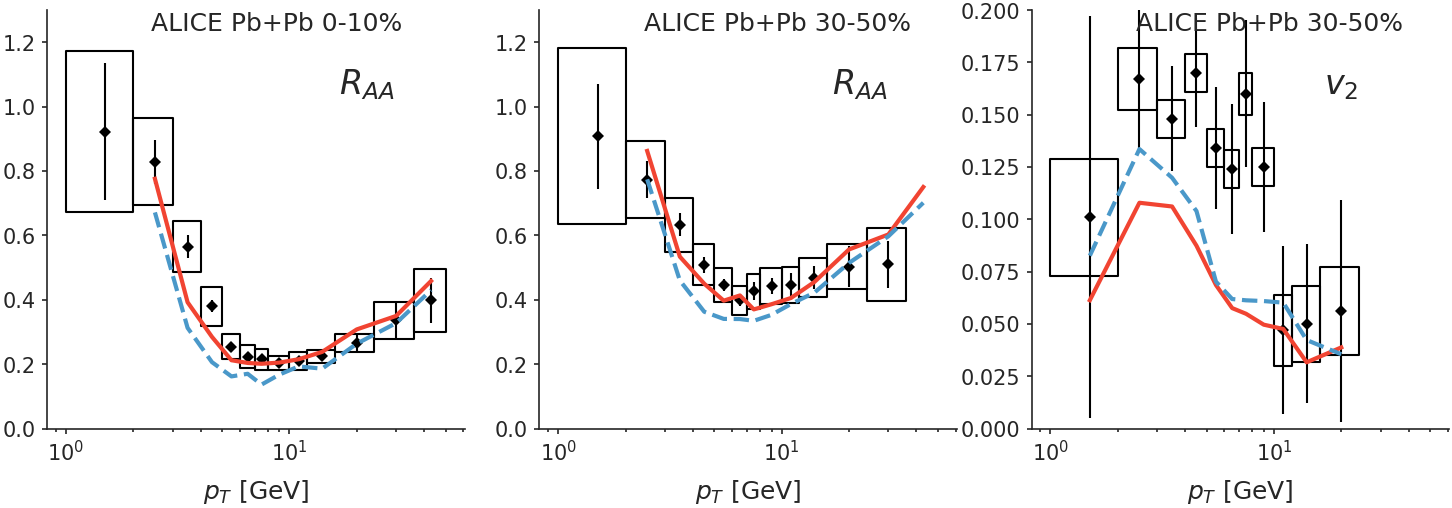
\includegraphics[width=\textwidth]{run_alphas_cut.png}
\caption{Effect of changing the switch scale between small-$Q$ diffusion modeling and large-$Q$ scattering modeling. $\mu=2$ is used. The red solid lines used a switching scale at $Q_{\textrm{switch}}^2 = 4 m_D^2$, and the blue dashed lines uses $16 m_D^2$.}
\label{fig:new:run-cut}
\end{figure}
\paragraph{Switching scale dependence} By construction, the energy loss should be insensitive to the switching scale between the small-$Q$ diffusion and the large-$Q$ scattering in the high energy, weakly coupled limit.
We check if this arguments holds for phenomenology application.
In figure \ref{fig:new:run-cut}, in additional to the default $Q_\textrm{cut}^2 = 4 m_D^2$ (red solid lines), we also uses $Q_\textrm{cut}^2 = 16 m_D^2$ (blue dashed lines) to model more probe-medium interaction by diffusion than scattering.
We found that the effect on high-$p_T$ observable is small.
Because the high-$p_T$ dynamics is dominated by the radiation energy loss, whose $Q_\textrm{cut}$ is indeed small as checked in chapter \ref{chapter:transport}.
Larger differences of $R_{AA}$ and $v_2$ is observed at low-$p_T$.
One reason for this is that the $Q_\textrm{cut}$ independence argument obtained for high energy partons does not work very well for low velocity partons.
Another reason is that despite the scattering dynamics and the diffusion dynamics has a matched diffusion constant (second moment of the momentum transfer), they are differed in all other momentum higher moment, in particular the drag (first moment).
Remember that the drag coefficient in the diffusion dynamics is not a direct input from the weakly coupled theory, but is determined by the Einstein relation.
The Einstein relation only guarantees that the diffusion dynamics eolves the system to the same equilibrium as the scattering dynamics, but the non-equilibrium path it takes can be very different from the scattering dynamics.

This $Q_\textrm{cut}$ dependence may be bad at first sight, but one knows that the weakly coupled scattering picture does not necessarily work for the phenomenological coupling regime ($g\sim 2$), while the diffusion dynamics can be extended to strongly coupled regime.
The $Q_\textrm{cut}$ actually parameters an important source of theoretical uncertainty in our modeling.

\begin{figure}
\centering
\includegraphics[width=\textwidth]{run_alphas_match.png}
\caption{Effect of changing the matching scale parameter $R_v$ ($\Delta k_\perp^2 = R_v Q^2$) between the vacuum-like shower and the medium-induced shower. $\mu=2$ is used. The red solid lines use $R_v =1$, while the blue dashed lines use $R_v = 1000$, which left the vacuum-like shower largely unmodified.}
\label{fig:new:run-match}
\end{figure}

\paragraph{Vacuum / medium-induced radiation matching scale dependence}
As explained, there is a separation treatment of radiation that lives in different regions of phase-space on the lund-diagram.
Accordingly, we need to subtract the vacuum radiation that overlapped with the medium-induced region in the Pythia event generator.
In our earlier transport study of heavy flavor \cite{Ke:2018tsh}, this subtraction is not included, therefore, we would like to demonstrate the impact of this mistreatment here.

In figure \ref{fig:new:run-match}, two calculations are shown. 
The red dashed lines stands the case where we removed vacuum-like radiations that satisfy $\Delta k_\perp^2 > Q^2$.
The blue solid lines are calculations without this subtraction.
The two calculations for $R_{AA}$ only differs for $p_T\gtrsim 20$ GeV, because only high-$p_T$ heavy quarks can undergo splittings that take long enough time to receive large medium corrections.
Also the difference is large for central collisions than for peripheral collisions, because medium effect for the latter is weaker.
No significant difference is observed for $v_n$.

\begin{figure}
\centering
\includegraphics[width=\textwidth]{run_alphas_local.png}
\caption{The impact of using ``local rate'' approximation. The red solid lines uses the default implementation; while the blue dashed line performs the rescatterings in an imaginary infinite box using locally defined temperatures to mimic the ``local rate'' approximation.}
\label{fig:new:run-local}
\end{figure}

\paragraph{Performance of the ``local rate'' approximation}
Finally, it is interesting to examine the effect of an ``local rate'' approximation of the radiative processes on the observables.
It approximates the radiation probability in a medium with slowly varying temperature by the integration of radiation rates defined in an infinite static box with the local temperature at each point.
One can also refers to it as the ``adiabatic'' approximation, because it really assumes the temperature variation is slow compared to the formation  time.

We know this approximation can be broken by the fast expansion of the QGP fireball, and would like to quantify the impact.
It is convenient to mimic the ``local'' approximation in our model, one can simply let the preformed-gluon rescattering procedure be done in an imaginary medium with the same temperature and flow velocity as those at the point of its production, instead of those in the evolving medium.
The results comparison are shown in figure \ref{fig:new:run-local}.
The local approximation is good except at very high-$p_T$ ($p_T > 30$ GeV).


\chapter{Bayesian model-to-data comparison}
\label{chapter:bayes}
We have discussed the modeling details of the heavy flavor transport in relativistic heavy-ion collisions, and have shown a comparison to data with rather a ``na\"ive'' guess of multiple parameters.
Till now, we have only varied a small subset of them to understand the model qualitatively.
In this section, we introduce the advanced statistical tool known as Bayesian analysis that can calibrate all parameters simultaneously to the experimental data.
For the full details of such an analysis, we refer the readers to this excellent dissertation on this subject \cite{Bernhard:2018hnz} in the context of heavy-ion collisions.

To facilitate the discussion, I define the problem for this chapter and introduce a few notations and terminologies.
We formulate the general task of a model-to-data comparison into the following form,
\begin{itemize}
\item A complex model $M$ with $n$ input parameters organized as a $n$-dimensional vector $\mathbf{p}$.
\item There exists a prior belief on the reasonable range of each parameter, known as the prior probability distribution, and for short ``$\mathrm{Prior}$''.
\item $n$ experimental measurements are organized as an observation vector $\mathbf{y}_{\exp}$ of dimension $m$, with given statistical and systematic uncertainties $\delta\mathbf{y}_{stat}$,$\delta\mathbf{y}_{sys}$.
\item The task is to infer the posterior probability distribution of $p$ ($\mathrm{Posterior}$), given the model $M$, the measurements $\delta\mathbf{y}_{\exp}\pm \delta \mathbf{y}$, and the $\mathrm{Prior}$.
\end{itemize}
The analysis proceeds in the following steps that are explained in each section.

\section{Model evaluation}
A prerequisite for this analysis is the ability to fast evaluate model $M$ at any point in the considered region of parameter space.
It is achieved by interpolating model calculations obtained at $N$ carefully designed parameter points.
This $N$ set of parameter vectors of length $n$ forms a so-called design matrix $\mathbf{D}$,
\begin{eqnarray}
\mathbf{D}_{N\times n} = 
\begin{bmatrix}
p_{11} & p_{12} & \cdots & p_{1n}\\
p_{21} & p_{22} & \cdots & p_{2n}\\
\vdots & \vdots & \ddots & \vdots \\
p_{N1} & p_{N2} & \cdots & p_{Nn}
\end{bmatrix}
\end{eqnarray}
where the first index is the label of different parameter set, and the second index labels different parameters.

We use an existing software \cite{lhs-r} of so-called Latin-Hyper-Cube design method \cite{MORRIS1995381} to determine the location of these points in parameter space.
It generates a semi-random design subject to the following constraints:
\begin{itemize}
\item The marginalized distribution on any parameter is a uniform distribution.
This is different from a grid design, where the marginalized distribution are spiky delta functions on the grid points.
\item The minimum distance between any two points in the parameter space is maximized.
This is different from a completely random design in which points may form tight clusters or leave sparsely occupied regions.
\end{itemize}
Usually, for a well-behaved model, the number of design points needed for a good interpolation increases linearly with the number of parameters $n$, in contrast to an exponential increasing with $n$ in a grid design.

The actually model evaluation on these points is the most time-consuming part of this analysis.
The outputs are organized into the observation matrix,
\begin{eqnarray}
\mathbf{Y}_{N\times m} = 
\begin{bmatrix}
y_{11} & y_{12} & \cdots & y_{1m}\\
y_{21} & y_{22} & \cdots & y_{2m}\\
\vdots & \vdots & \ddots & \vdots \\
y_{N1} & y_{N2} & \cdots & y_{Nm}
\end{bmatrix}
\end{eqnarray}
where the first index is the label of different parameter set, and the second index labels different observables.
The design matrix $\mathbf{D}$ and the observations matrix $\mathbf{Y}$ help to train a general interpolator to infer the calculated observables at any given parameter value.

\section{Data reduction}
The model $M$ is a mapping of an $n$-dimensional vector to an $m$-dimensional vector. 
One can certainly construct an array of independent $m$ scalar mappings, and interpolate each of them.
However, this na\"ive construction does not make use of the intrinsic correlations/structures in the training data, and can be very inefficient for practice usage.
Considering an observation with two values of $R_{AA}$ and $v_2$. Usually, the larger the $R_{AA}$ the model predicts, the smaller the $v_2$ is, and thus an anti-correlation is expected.
If one build interpolators for them independently, the interpolation uncertainties are also going to be independent, which does not reflect the correlation information.
However, if one interpolates the linear combinations $a R_{AA} \pm b v_2$; then a wise choice of $a, b$ significantly reduces the correlation between these two ``newly'' constructed observables.

The principal component analysis (PCA) is a systematic way to implement this idea.
The original vectors of observables are transformed into the principal-component (PC) space, with each PC a specific linear combination of the original observables, so that the covariances between the newly defined observables (the PCs) vanish.
Mathematically, this is the same as finding the singular value decomposition (SVD) of $\mathbf{\tilde{Y}}$. 
$\mathbf{\tilde{Y}}$ is the standardized observation matrix $\mathbf{Y}$,
\begin{eqnarray}
\tilde{y}_{ij} = \frac{y_{ij} - \mu_j}{\sigma_j}
\end{eqnarray}
with $\mu_j$ and $\sigma_j$ the mean and the standard deviation of column $j$.
Then the SVD proceeds as,
\begin{eqnarray}
\tilde{\mathbf{Y}}_{N\times m} = \mathbf{U}_{N\times N} \mathbf{\Sigma}_{N\times m} \mathbf{V}_{m\times m}.
\end{eqnarray}
Here $\mathbf{\Sigma}$ only contains the variance of each PCs on its diagonal.
The PCs are defined as the components after the $V$ transformation.
\begin{eqnarray}
z = \mathbf{V}y
\end{eqnarray}
It is evident that the covariance matrix of the $z$ observables is diagonalized,
\begin{eqnarray}
\mathrm{Var}(z_i, z_j) = \frac{1}{N}V_{ii'}\tilde{Y}_{ki'}V_{jj'}\tilde{Y}_{kj'} = \frac{1}{N}V\tilde{Y}^T\tilde{Y}V^T = \frac{1}{N}\mathbf{\Sigma}.
\end{eqnarray}
So different PCs are orthogonalized.

A data reduction is another benefit of using PCA.
Suppose we have sorted the variance in $\mathbf{\Sigma}$ from maximum to minimum.
For data with pronounced structures, often the first few PCs take into account the majority of the data variance.
Practically, a truncated set of PCs already gives a good representation of the original data, and this dramatically reduces the computations necessary for interpolating a large number of observables.
Finally, one can always go back from the PC space to the original space by the inverse transformation $y = V^{-1} z$.
The PCA software is provided by \cite{sklearn_api}.

\section{Model emulator}
With limited information on a finite number of design points contained in the matrices $D$ and $M$, the original mapping is approximated by a model emulator (a surrogate model) using a Gaussian Process (GP).
The Gaussian Process provides a non-parametric interpolation for scalar function with one or high dimensional input.
We shall let the readers refer to \cite{rasmussen2006gaussian} for the technical details and only summarize the basics of the Gaussian Process.

\paragraph{Gaussian Process} Take a uni-variate case as an example. Given an array of input and an array of output, polynomial interpolation is a common way to interpolate the data.
However, polynomial interpolation only uses local information of the grid, and its performance can be sensitive to the error of the output, e.g., statistical fluctuation in the simulation.
Moreover, it is hard to work with a Lain-hypercube design because the design points are not arranged on a regular grid.
In contrary, a GP does not make any assumption on the functional form of the interpolation but infers the output at a particular input based on how its output correlates with given outputs at other input points.
Mathematically, one assumes that elements of the predicted output $\mathbf{y}^*$ at input $\mathbf{x^*}$ and the known outputs $\mathbf{y}_{\textrm{train}}$ at the training points $\mathbf{x}_{\textrm{train}}$ form a multi-variate normal distribution,
\begin{eqnarray}
\begin{bmatrix}
\mathbf{y}^* \\
\mathbf{y}_{\textrm{train}}
\end{bmatrix}
\sim
\mathcal{N}\left(
\begin{bmatrix}
\mathbf{\mu}^* \\
\mathbf{\mu}_{\textrm{train}}
\end{bmatrix},
\begin{bmatrix}
\mathbf{\Sigma}(\mathbf{x}^*, \mathbf{x}^*)& \mathbf{\Sigma}(\mathbf{x}^*, \mathbf{x}_{\textrm{train}}) \\
\mathbf{\Sigma}(\mathbf{x}_{\textrm{train}}, \mathbf{x}^*)& \mathbf{\Sigma}(\mathbf{x}_{\textrm{train}}, \mathbf{x}_{\textrm{train}})
\end{bmatrix}
\right)
\end{eqnarray}
Without a loss of generality, one often standardizes the training data so that the mean values $\mathbf{\mu}^*$ and $\mathbf{\mu}_{\textrm{train}}$ are zero.
The $\mathbf{\Sigma}$s form the covariance matrix, and each of them has the same shape of the outer product of its two arguments.
Its matrix-element (the kernel function) are parametric, and one often takes a squared exponential form,
\begin{eqnarray}
\Sigma_{ij} = k(x_i, x_j) = \sigma^2 \exp\left(-\frac{(x_i-x_j)^2}{2l^2}\right).
\end{eqnarray}
$\sigma^2$ is the auto correlation and $l$ is the correlation length.
The covariance decays exponentially with the squared separation of the two input points.
In such a way, points that are close in inputs will also be close in outputs, and points that are far apart are effectively uncorrelated.
The squared exponential form is not the only possible kernel function; people have designed more sophisticated choices with more parameters for various problems. 

\paragraph{Conditioning a Gaussian Process} The outputs at training points are known.
Therefore, the probability distribution of $\mathbf{y}^*$ is obtained by conditioning the training outputs on their actual values,
\begin{eqnarray}
\mathbf{y}^* \sim &&\mathcal{N}\left(
\mathbf{\Sigma}(\mathbf{x}^*, \mathbf{x}_{\textrm{train}} )
\mathbf{\Sigma}^{-1}(\mathbf{x}_{\textrm{train}}, \mathbf{x}_{\textrm{train}} )\mathbf{y}_{\textrm{train}},\right.\\\nonumber
&&\left.
\mathbf{\Sigma}(\mathbf{x}^*, \mathbf{x}^*) - 
\mathbf{\Sigma}(\mathbf{x}^*, \mathbf{x}_{\textrm{train}} )
\mathbf{\Sigma}^{-1}(\mathbf{x}_{\textrm{train}}, \mathbf{x}_{\textrm{train}} )
\mathbf{\Sigma}(\mathbf{x}_{\textrm{train}},\mathbf{x}^*)
\right)
\end{eqnarray}
Note that the conditional multivariate normal distribution is still a normal distribution, with modified mean and covariance matrix.
One can check that if the predicted input approaches one of the training inputs, the distribution of the output approaches a $\delta$-function (as the limit of a narrow Gaussian) at the training output.

\paragraph{Hyperparameters and training} We have not discussed the parameters in the kernel function $k(x, x')$ too much yet.
For now, they are the auto-correlation $\sigma^2$ and the correlation length $l$. 
They are known as hyper-parameters (denoted as a vector $\mathbf{\theta}$), and should in principle, be treated as unknown parameters in the calibration.
But a common practice to reduce the complexity is to fix the hyper-parameters at a set of ``optimal values'' by minimizing the loss function $\mathcal{L}$,
\begin{eqnarray}
\mathcal{L} = -\ln p(\mathbf{y}|\mathbf{\theta}) = \frac{1}{2}\ln \det \mathbf{\Sigma}(\mathbf{\theta})  + \frac{1}{2}\mathbf{y}^T \mathbf{\Sigma}(\mathbf{\theta})^{-1} \mathbf{y} + \frac{N}{2}\ln(2\pi)
\end{eqnarray}
where $\mathbf{y}$ is the (PCA transformed) training data, and $N$ is the number of training points.
The minimization process is referred as ``training'' a Gaussian Process emulator.

\paragraph{Inference with uncertainty quantification} Unlike the polynomial interpolation, a GP does not provide a single estimation of the output but infers the probability distribution of the predicted outputs by predicting both the mean and the covariance matrix.
It is a huge advantage of the Gaussian Process to quantify its interpolation uncertainty.

\paragraph{Validation} Though the training process includes a penalty for over-fitting the data, whether the trained GP has an over-fitting problem can only be checked by validation.
In a validation procedure, one performs model calculations at novel points in the parameter space that is not used to train the GP; then, compare the GP's prediction $y_i \pm \sigma_i$ to the model calculation $y_{\textrm{validate}, i}$.
If an emulator is trained to work properly, then the standardized deviation $(y_i - y_{\textrm{validate}, i})/\sigma_i$ should follow approximately a standard normal distribution.

\paragraph{Multivariate inputs and outputs} The GP formulation can be easily generalized to higher-dimensional inputs by specifying a multidimensional kernel function.
For high dimensional outputs, one first applies the PCA analysis introduced in the previous section and the build individual GPs for each of the first $N_{PC}$ principal components that take most of the data variance.

\section{Bayes' theorem and Markov chain Monte Carlo}
With the model emulator $M$ (we are using the same symbol as the model, but one should always remember that the emulator is only a fast surrogate of the original model and comes with uncertainty), we apply Bayes' theorem, the essence of the statistical analysis.
Bayes' theorem provides a quantitative way to update the knowledge of model parameters with empirical observations,
\begin{eqnarray}
\mathrm{Posterior}(\mathbf{p}|M, \mathbf{y}_{\textrm{exp}}) \propto \mathrm{Likelihood}(\mathbf{y}_{\textrm{exp}}|M, \mathbf{p})\times\mathrm{Prior}(\mathbf{p}).
\end{eqnarray}
It states that the posterior probability distribution of parameters, given the model and experimental measurements, is proportional to the likelihood of describing the experiments with the model using this set of parameters, times the prior belief of the distribution of the parameters.
The likelihood function is often assumed to be a multivariate Gaussian,
\begin{eqnarray}
\mathrm{Likelihood}(\mathbf{p}) &=& (2\pi)^{-\frac{m}{2}} (\det|\Sigma|)^{-\frac{1}{2}} \exp\left\{-\frac{1}{2}\Delta \mathbf{y}^T \mathbf{\Sigma}^{-1} \Delta \mathbf{y}\right\}, \\ 
\Delta \mathbf{y} &=& \mathbf{y}(\mathbf{p}) - \mathbf{y}_{\textrm{exp}}
\end{eqnarray}
where the $\mathbf{y}(\mathbf{p})$ is the model emulators' prediction at parameter point $\mathbf{p}$, $m$ is the number of observables.
The prior distribution is often a multi-dimensional uniform distribution within a reasonable range. 
The covariance matrix contains various sources of uncertainties from both theory and experimental side.

\paragraph{A model dependent statement}One always defines a posterior with a given model; therefore, even the extraction of theoretically well-defined quantities can be affected by different dynamical modeling assumptions/approximations.
On the one hand, the ultimate solution is, of course, to improve the physical accuracy of the model.
On the other hand, one could use a flexible model or models with different (but reasonable) assumptions to extract the same quantity to establish a level of theoretical uncertainty.

\paragraph{The covariance matrix} covariance matrix is decomposed into different contributions,
\begin{eqnarray}
\mathbf{\Sigma} = \mathbf{\Sigma}_{\textrm{stat}} + \mathbf{\Sigma}_{\textrm{sys}} + \mathbf{\Sigma}_{\textrm{emulator}} + \mathbf{\Sigma}_{\textrm{truncation}} + \mathbf{\Sigma}_{\textrm{model, sys}}
\end{eqnarray}
\begin{itemize}
\item The statistical co-variance takes the diagonal form, $\mathbf{\Sigma}_{\textrm{stat}} = \delta_{ij}\delta\mathbf{y}_{\textrm{stat}, i}^2$. 
$\delta\mathbf{y}_{\textrm{stat}, i}$ is the experimental statistical uncertainty.
\item The experimental systematic uncertainties $\mathbf{\Sigma}_{\textrm{sys}}$ can be correlated for different observations, so generally its off-diagonal elements are non-zero,
\item The emulator covariance $\mathbf{\Sigma}_{\textrm{emulator}}$ is the prediction covariance of the GPs in the PC space and then transformed into the physical space.
\item The truncation covariance $\mathbf{\Sigma}_{\textrm{truncation}}$ take those less important principal components that are not being emulated by GPs into account. 
Its variance is first computed in the PC space and then transformed back to the physical space.
\item Finally, $\mathbf{\Sigma}_{\textrm{model, sys}}$ stands for the model uncertainty. 
It is always present but is hard to quantify using the model itself.
Therefore, the previous study \cite{Bernhard:2018hnz} assign a variable model systematic uncertainty parameter $\sigma$, and this parameter will be treated as uncertainty in the calibration as well.
The $\sigma$ stands for a uniform model uncertainty fraction on each principal component and is added to the emulator prediction covariance.
The $\sigma$ parameter is given an information prior distribution $P(\sigma) \propto \sigma^2 e^{-\sigma/0.05}$. Meaning an expectation of $15\%$ model uncertainty.
The exact origin of this model uncertainty is unknown, but it plays a row as a ``regulator'' in the fitting process to prevent the model trying to explain features that can never be described better than a $\sigma$ level precision.
\end{itemize}

\paragraph{Marginalize the posterior distribution} The resultant posterior distribution is a function of $n$ parameters.
To answer what is the probability distribution of one parameter folded with the uncertainty from other parameters, one looks at the marginalized distribution with the other $n-1$ parameters integrated out.
A Markov chain Monte Carlo (MCMC) sampling of the posterior function performs the marginalization.
The MCMC evolves an ensemble of $n$-dimensional walkers to thermalize to the target posterior distribution.
Then, one obtains the one-parameter marginalization by projecting the ensemble onto one dimension.
Similarly, a marginalization of the joint-distribution of two or more parameters can be obtained similarly.
The MCMC software is developed by \cite{emcee}.

\chapter{Results}
\label{chapter:results}
In this chapter, we apply the advanced statistical tools to the heavy-flavor transport model and extract the heavy quark transport coefficients.
I would like to present this in a two step processes to show the improvements of the lastest extraction.



\paragraph{A list of experimental data}
\section{Lessons from earlier extractions of $\hat{q}_Q$}
In an earlier publication [], we used a linearized Boltzmann model with the coherence factor approach to implement the LPM effect.
The heavy quark initial momentum dsitribution is obtained from the FONLL calculation.
We have already commented on the advantages and disadvantages of these choices.
Two different set of nuclear PDF $EPPS$ and $nCTEQ15$ are used to represent the uncertainty from the cold nuclear matter effect in the $\hat{q}$ extraction.

Regarding model parameters, the one parameter for the perturbative elastic and inelastic scatterings is controlled by $1/3 < \mu < 4$ in the running coupling. 
There is an additional pure diffusion process with a diffusion constant $\kappa_{NP}$ parametized to peak at low temperature and low energy, in order to mimic certain non-perturbative coupling between a low energy probe and the medium near $T_c$,
\begin{eqnarray}
\kappa_{NP} = T^3 \kappa_D \left(x_D + (1-x_D)\frac{1\textrm{ GeV}{}^2}{ET}\right).
\end{eqnarray}
The $0<\kappa_D<8$ parameter is the overall strength of the diffusion, and the $0<x_D<1$ controls the degree of energy-temperature dependence.
One can see that in the heavy quark limit $M\rightarrow \infty$, this parametrization becomes independent of mass.
An additional parameter is the in-medium energy loss starting time $\tau_0$ that is allowed to be tuned between $0.1$ fm/$c$ to $1.0$ fm/$c$ (before the onset of hydrodynamics).
The reason is we lack a quantitative description of the production of color charge in the initial stages.
This starting time is a simple approximation that interactions is only turned on after $\tau_0$ when the color carries is assumed to approach a Boltzmann distribution.


The design of the four dimensional parameter space  $(\tau_0, \mu, \kappa_D, x_D)$ has 80 design points.
The computation is carried on the distributed computing system Open Science Grid [] using about a million CPU hours.
The observabes on which we calibrated are listed in tables \ref{table:ALICE-obs} and \ref{table:CMS-obs}. 
Including, $p_T$ dependent $D$-meson nuclear modification factor $R_{AA}$ and $p_T$ dependent (event-shape-engineered) azimuthal anisotropy $v_2$.
CMS measurements of the $B^{\pm}$-meson $R_{AA}$ is also included to constrain the mass dependence of the transport coefficients.

\begin{figure*}
\includegraphics[width=.49\textwidth]{observables_design.pdf}
\includegraphics[width=.49\textwidth]{observables_posterior.pdf}
\caption{Left: the prior, i.e. the full range of calculations in parameter space. Right: the posterior, i.e. observables sampled from model emulators after calibration. In both figures, blue (green) lines are calculations with {\tt EPPS} ({\tt nCTEQ15np}) nuclear PDF.}\label{plots:deisgn_posterior_obs}
\end{figure*}

The prior and the posterior of the observables before and after the calibration is shwon in figure \ref{plots:deisgn_posterior_obs}.
blue stands for using {\tt EPPS} nuclear PDF and green stands for using the {\tt nCTEQnp}  nuclear PDF.
We found that the model after the calibration provide a good description of $R_{AA}$ and $v_2$ at the intermediate $p_T$ of the ALICE experiments.
But it does not reproduce the fast uprising shape of $R_{AA}$ at high-$p_T$ of the CMS experiment.
In addition, the model seem to under estimate the high-$p_T$ $v_2$ of the $30-50\%$ centrality bin measured by CMS.
The model is able to explain the correlation between the D-meson $v_2$ and the event-shape, though there are still large fluctuation in the data.
The use of different nuclear PDFs has a negligible effect on $v_2$, but does affect the $R_{AA}$ at small and large $p_T$.
Another thing worth noting that is that the $D$ and $B$ meson $R_{AA}$ are described at the same time.

\begin{figure}
\centering
\includegraphics[width=.7\textwidth]{posterior.pdf}
\caption{Marginalized postrior probability distribution of model parameters. Diagonal plots show the marginalization on a single parameter. Off diagonal plots show the pair correlation between parameters. Blue (Geen) lines and lower (upper) off diagonal plots correspond to the extraction using EPPS (nCTEQ15np) nuclear PDF.}\label{plots:posterior}
\end{figure}

The inferred posterior probability distribution of the parameters is shown in the figure \ref{plots:posterior}.
The diagonal plots show single parameterized distributions, and the off-diagonal ones displays the two-parameter correlations.
We split the results that use different nuclear PDFs into the upper (EPPS, green heat map and lines) and lower (nCTEQ15np, blue heat maps and lines) triangles.
One notices that results from different nuclear PDF are consistent within the uncertainty; therefore, from now on I shall not stress on any differences between these two set of results, but combine them into a single distribution to fold in the PDF uncertainty.
The favored parameters are $\mu \sim 0.6$ and $\kappa_D \sim 0.4$, indicating a large in-medium $\alpha_s$ and a small additional diffusion.
The typical value of the $\alpha_s$ is, in fact, so large that let one worried about the use of weakly-couple based approaches.
For example, $\alpha_s(0.6\pi T)$ at $T=300$ MeV is 0.67, corresponding to $g \approx 3$. 
And the screening mass $m_D \sim 3.6 T$ is even larger than the average energy of the thermal partons $3T$. 
In the discussion of the next section, we will see that this problem can be slightly alleviated, once we use the improved implementation of the LPM effect and implement a separation of soft-modes into the diffusion constant, though $g$ is still large.

\begin{figure}
\includegraphics[width=\columnwidth]{qhat_p_T.pdf}
\caption{Posterior range of the heavy quark transverse momentum broadening parameter $\hat{q}$ from Equation \ref{eq:qhat}. The results include the uncertainty from using different nuclear PDFs. Blue boxed region is for bottom quarks and red slashed region for charm quarks.}\label{fig:posterior_qhat}
\end{figure}

\paragraph{Transport coefficients} In this analysis, the heavy quark transport coefficient $\hat{q}$ is computed from adding up the momentum broadening from both the scattering and the parametric diffusion,
\begin{eqnarray}\label{eq:qhat}
\hat{q} &=& 2T^3\kappa_D\left(x_D + (1-x_D)\frac{\textrm{GeV}^2}{ET}\right) + \hat{q}_{\textrm{el}}.
\end{eqnarray}
In a perturbative definition of the transport coefficients, the inelastic process does not contribute to heavy quark transport coefficient at leading order. 
In figure \ref{plots:posterior_qhat}, the 90\% credible region of $\hat{q}$ is shown as a function of temperature at a fixed energy (left), and as function of energy at a fixed temperature (right).
Results for charm (red) and bottom (blue) quarks are labeled by different colors.
The mass difference only causes a small difference in $\hat{q}$.

\begin{figure}
\includegraphics[width=\columnwidth]{qhat_compare.pdf}
\caption{Posterior range of the heavy quark transverse momentum broadening parameter $\hat{q}$. The shaded region indicates a previous extraction using the improved-Langevin model [].}\label{fig:compare_qhat}
\end{figure}

\paragraph{Comparison to results from an improved-Langevin model}
The same transport coefficient is also extracted using the improved-Langevin model [].
It includes a diffusion modeling of the elastic interacton, a high-twist single gluon emission rate, and a similar routine to implement multiple radiations.
This model is then coupled to the same medium as the one used here and compared to the same set of observables as this work does.
The resultant posterior (for charm quark only) is shown as the shaded region in figure \ref{fig:compare_qhat}.
We see that the $\hat{q}$ extracted using the two models only overlap at the boundary of the credible region.
Their difference is comparable to the uncertainty band of either model, while both models provide a reasonable description of the data.
This suggests the theoretical uncertainty that comes from the assumption between the probe and the medium is a significant one.
The ability to tune a switching scale parameter in the new model intends to include this type of theoretical uncertainty.

\section{Calibration using the improved transport model}
Finally, we apply the improved model to the extraction of the heavy quark transport coefficients.
As a summary of the improvements:
\begin{itemize}
\item A more sophisticated implementation of the LPM effect to reduce modeling uncertainty of the radiative process;
\item An interpolation of the diffusion picture and the scattering picture to take into account modeling uncertainty.
\item Separating the high-virtuality evolution and the low-virtuality transport equation at a medium scale.
\end{itemize}

\paragraph{Model parameters}
In the new analysis, we try to include as many theoretical uncertainty as possible, so we have much more parameters than the two previous studies.
They are listed in table \ref{table:new:prior}.
\begin{itemize}
\item The first parameter is again the energy loss starting time $\tau_i$.
In this analysis, we are comparing to data at two collision energies and the hydrodynamic starting time $\tau_0$ varies from $1.2$ fm/$c$ to $0.6$ fm/$c$.
To account for this differences, we use the ratio $\xi = \tau_i/\tau_0$ as the single parameter for both energies.
It means that after $\xi$ fraction of the hydrodynamization time, the color density is assumed to be large enough to apply the linearized transport  model.
\item The second parameter is switching scale parameter $1.0 < c < 10.0$ in $Q_{\textrm{cut}}^2 = c m_D^2$. For a typical coupling $g\sim 2$, $Q_{\textrm{cut}}$ is then varied from about $2T$ to $7T$.
\item The third parameter $0<R_v<7$ controls the matching condition between the vacuum-like radiation and the medium-induce radiation $\Delta k_\perp^2 = R_v Q^2$.
At $R_v = 0$, the vacuum-like radiation is completely forbidden once it interacts with the medium; for $R_v \gg 1$, the vacuum-like radiation is effectively unmodified.
\item The $0.6 < \mu < 10$ parameter controls the in-medium strong coupling $\alpha_s(\max\{Q, \mu\pi T\})$.
\item The rest of the six numbers $K,a,b,p,q, \gamma$ parametrizes a correction to the weakly coupled transport coefficient $\hat{q} + \Delta\hat{q}$, $\hat{q}_L + \Delta\hat{q}_L$,
\begin{eqnarray}
\Delta\hat{q} &=& \frac{K T^3}{\left[1+\left(a\frac{T}{T_c}\right)^p\right]\left[1+\left(b\frac{E}{T}\right)^q\right]}, \\
\Delta\hat{q}_L &=& \left(\frac{E}{M}\right)^\gamma \frac{\Delta\hat{q}}{2}
\end{eqnarray}
$0 < K < 15$ is the overall magnitude of the correction. 
The deviation from the $T^3$ dependence and the energy dependence are parametrized using two dimensionless combinations $T/T_c$, and $E/T$.
The $\gamma$ parameter varied from $-1$ to $1$ allows the correction to be anisotropic.
Note that such a construction goes back to an isotropic diffusion when velocity approaches zero ($E\rightarrow M$).
\end{itemize}
\begin{table}
\centering
\caption{Prior range of parameters}\label{table:new:prior}
\begin{tabular}{ccc}
\hline
Symbol & Description & Range \\
\hline
$\xi = \frac{\tau_0}{\tau_{\textrm{hydro}}}$ & Energy loss starting time & (.1, .9) \\
$c = \frac{Q_{\textrm{cut}}^2}{m_D^2}$ & Soft / hard switching scale & $(.1, 10.)$ \\
$R_v$ & Vacuum / Medium mathcing scale & $(0,7)$\\
$\mu$ & Running $\alpha_s$ stops at $Q = \mu\pi T$ & $(.6, 10)$ \\
$K$ & Magnitude of $\Delta \hat{q}/T^3$ & $(0, 15)$\\ 
$p$ & \multirow{2}{*}{$E$-dependence of $\Delta \hat{q}/T^3$} & $(-2, 2)$\\ 
$a$ &  & $(-1, 1)$\\ 
$q$ & \multirow{2}{*}{$T$-dependence of $\Delta \hat{q}/T^3$}  & $(-.5, 3)$\\ 
$b$ &   & $(-.5, 3)$\\ 
$\gamma$ & $\Delta \hat{q}_L = (E/M)^\gamma\Delta \hat{q}_L$  & (-1, 1)\\ 
\hline
\end{tabular}
\end{table}

\paragraph{Design and prior} 
We chosoe to give $\ln c, \ln R_v, \ln \mu, \ln a$ and $\ln b$ an uniform design and a uniform prior.
Therefore, the original parameter will have a non-uniform design and prior distribution.
The reason is that these parameters either causes a logarithmic slow change in the model and its prior uncertainty is large that it is allowed vary by orders of magnitude.
For example, the $\mu$ parameter enters the logarithmic running of $\alpha_s$ and we can rewrite the maximum possible $\alpha_s$ as,
\begin{eqnarray}
\alpha_{s,\max}(T) = \frac{2\pi}{9}\frac{1}{\ln(\mu) + \ln(\pi T/\Lambda_{\textrm{QCD}})}
\end{eqnarray}
Therefore, we assign a uniform prior to $\ln(\mu)$ so that $\alpha_s$ also varies notable within the prior range.
For the $c$ and $R_v$ parameter, we have seen in the previous benchmark calculation that the $R_{AA}$ and $v_2$ predictions depends fairly weak on the choice of these parameter, therefore they are also given a logarithm prior.
For the $a$ and $b$ parameters, one notice that asymptotically largeness or smallness of these numbers do not change the value of $\Delta \hat{q}$ notably.
By applying the logarithmic prior and design, we can explore both the large and small limits of these numbers while still have enough design points to control the interpolation uncertainty in the physical interesting regions ($a$ and $b$ are of order one). 

\begin{figure}
\centering
\includegraphics[width=.4\textwidth]{qhat_prior.png}\includegraphics[width=.4\textwidth]{ER_prior.png}
\caption{•}
\label{fig:new:design-qhat}
\end{figure}

We sampled 250 design points and 50 validation points. 
Combining $\mu, K, p, q, a, b$ and $\gamma$, the prior region of the heavy quark transport parameters are plotted function of temperature and energy in figure \ref{fig:new:design-qhat}. 
On the left, 250 design's $\hat{q}$ as function of temperatures are shown  (using charm mass for demonstration).
Each subplot shows quark energy at $1.4$ GeV, $11.4$ GeV and $101.3$ GeV.
The prior range of $\hat{q}$ varies over an order of magnitude.
On the right of the figure, we show the ratio $2\hat{q}_L/\hat{q}$ to indicated the degree of anisotropy of the transport parameters.

The computations of the model on both the design points and the validation points are performed on the NERSC super-computing system using over two million CPU hours.
The prior observables are shown in figure \ref{fig:new:obs_prior_LHC} at LHC energy $\sqrt{s}$ = 5.02 TeV and in figure \ref{fig:new:obs_prior_RHIC} at RHIC energy $\sqrt{s} = 200$ GeV.
In additional to LHC dataset used in the last calibration, we also include a dataset at RHIC energy measured by the STAR Collaboration [].
We choose two observables at RHIC, namely D meson $R_{CP}$ and $v_2$. 
The new one, $R_{CP}$, is defined as the $N_{\textrm{bin}}$ normalized ratio between the D meson yield in a smaller centrality class $C$ to a larger centrality class $P$,
\begin{eqnarray}
R_{\textrm{CP}} = \frac{dN_\textrm{C}/dp_T N_{\textrm{bin,P}}}{dN_\textrm{P}/dp_T N_{\textrm{bin,C}}}.
\end{eqnarray}
Using the nuclear data as a reference has the advantage of canceling certain theoretical uncertainties, such as the nuclear PDF (if its impact-parameter dependence is neglected) and possible modifications to the initial production mechanism in the nuclear environment.
A problem we found at RHIC energy is that even varying wildly the parameters, the very low-$p_T$ $R_{CP}$ is not well covered by the calculation. 
This indicates the model will have to be improved in this region of $p_T$, possible a more up-to-date dynamical hadronization model.
Our temporary solution is to only include the STAR $R_{CP}$ data above $5$ GeV in the calibration.

\begin{figure}
\centering
\includegraphics[width=\textwidth]{obs_prior_LHC.png}
\caption{•}
\label{fig:new:obs_prior_LHC}
\end{figure}

\begin{figure}
\centering
\includegraphics[width=\textwidth]{obs_prior_RHIC.png}
\caption{•}
\label{fig:new:obs_prior_RHIC}
\end{figure}

\paragraph{Emulator validation} 
The validation is performed by comparing the emulator trained on the 250 design points to the actual calculation on the 50 validation points.
We visualize the validation in figure \ref{fig:new:validation}.
In the top row, the emulated $v_2$ (left) and emulated $R_{AA}$ (right) are compared with the model calculations, and the data from different experiments and centrality has been labeled by different colors.
The emulated values strongly correlates with the true calculations around the the $y=x$ line.
Most points hit off the line, meaning the emulator is not 100\% accurate.
To see if the uncertainty is accounted for, we scatter plot the emulator's prediction uncertainty ($1\sigma$, $y$ axis) versus the absolute deviation between the prediction and the calculation (the $x$ axis).
The dashed line defines the shaded region where the true deviation is large than $\pm 3\sigma$.
We found that over $99\%$ of the prediction are within the $3\sigma$ region.
Therefore, for most cases the emulator correctly estimates its uncertainty  and therefore prevents over-fitting.

\begin{figure}
\centering
\includegraphics[width=.8\textwidth]{validation.png}
\caption{•}
\label{fig:new:validation}
\end{figure}

\paragraph{Co-variance matrix} 
From chapter \ref{chapter:bayes}, the co-variance matrix has the structure
\begin{eqnarray}
\Sigma = \Sigma_{\textrm{emulator}} + \Sigma_{\textrm{truncation}} + \Sigma_{\textrm{stat}} + \Sigma_{\textrm{sys}} + \Sigma_{\textrm{model, sys}} 
\end{eqnarray}
The construction of these terms are straight forward, except for the systematic covariance $\Sigma_{\textrm{sys}}$ of the experimental data.
Usually, experiments publish the marginalized uncertainty on each observable point $\delta y_{sys}$ (for example, $R_{AA}$ of a certain centrality at a single $p_T$ bin), and may specify the nature of the uncertainty as ``correlated'' or ``uncorrelated''.
The correlation among uncertainties is important as it directly affects the interpretation of the quality of fit.
For instance: a fit with $+5\%$ deviations on each of the $N$ data points will be penalized by a factor $e^{-N(0.05 y)^2/\delta y^2}$, assuming uncorrelated uncertainty; while it will only be penalized by $e^{-(0.05 y)^2/\delta y^2}$ if one assumes fully correlated uncertainty.
This is because fully correlated uncertainty allows data to be systematically deviation from a trend.

However, we the lack the information to construct the full covariance matrix from $\delta y_{sys}$.
In this study, we simply parametrize the correlation as function of observables (labeled by $\alpha, \beta \in \{R_{AA}, v_2, R_{CP}\}$), centrality labeled by $m,n$ and transverse momentum (labeled by $i,j$),
\begin{eqnarray}
\mathbf{\Sigma}_{\textrm{sys}} = \delta_{\alpha\beta} C_{mn}  \exp\left\{-\frac{1}{2 L_{\textrm{corr}}^2} \left(\ln\frac{p_{T, i}}{p_{T, j}}\right)^2 \right\} \times \sigma^{\alpha m}_{\textrm{sys}, i}\sigma^{\beta n}_{\textrm{sys}, j}.
\end{eqnarray}
So, the covariance is zero if there are different observables or measurements from different experiments or different particle species.
The centrality correlation $C_{mn}$ is only applied to $R_{AA}$ and $R_{CP}$ as these quantities across different centrality shares the same baseline reference, so a fraction of their uncertainty must be correlated across-centrality. 
By default, $C_{m=n}=1$ and $C_{m\neq n}=0.3$.
The correlation in the $p_T$ dimension is assumed to be a Gaussian in the $\ln p_T$ space with correlation length $L_{\textrm{corr}}$.
We use $\ln p_T$ based on the consideration that the original of these uncertainty should not be sensitive to the linear change of $p_T$ as the there is no other scale present.
The default correlation length is $1$, meaning the uncertainty is effectively uncorrelated with measurements at a $p_T$ $2.7$ times larger or smaller.
Finally, this correlation modulation is applied to the completely correlation case of the systematic uncertainty $\sigma^{\alpha m}_{\textrm{sys}, i}\sigma^{\beta n}_{\textrm{sys}, j}$.

This construction is entirely parametric, except for the direct experimental inputs $\sigma^{\alpha m}_{\textrm{sys}, i}$.
We hope that future measurements will provide more information on the co-variance structure of the published systematic uncertainties.
In the actually calibration, we will also change a few default parameters to see if the extracted physical parameters are sensitive to the detailed construction of $\Sigma_{\textrm{sys}}$.

\begin{figure}
\centering
\includegraphics[width=\textwidth]{obs_posterior_LHC.png}
\caption{•}
\label{fig:new:obs_posterior_LHC}
\end{figure}

\paragraph{Posterior observables} The global level of agreement between the calibrated model and the data is shown in figure \ref{fig:new:obs_posterior_LHC} at the LHC energy, and figure \ref{fig:new:obs_posterior_RHIC} at the RHIC energy.
The black dashed lines show the median prediction, while the blue bands stands for $90\%$ credible region.
We remind the reader that because of the model predicts anti-correlation between $R_{AA}$ and $v_2$, the lower and upper bounds of the uncertainty bands are also anti-correlated.
For example, a line that is close to the higher bounds in $R_{AA}$ is likely to be lose to the lower bounds in $v_2$.

Both the $D$-meson and the $B$-meson $R_{AA}$ at the LHC energy are well described by the calibrated model, while $v_2$ is systematically below the data.
Large separation between the event-engineered $v_2$ is observed, 
At the RHIC energy, $v_2$ has a better agreement. 
The magnitude of $R_{CP}$ at $p_T> 5$ GeV \footnote{Remember that the model is calibrated on the three data points above $p_T=5$ GeV} and its centrality dependences is correctly reflected, though the shape is too flat compared to the data.

\begin{figure}
\centering
\includegraphics[width=\textwidth]{obs_posterior_RHIC.png}
\caption{•}
\label{fig:new:obs_posterior_RHIC}
\end{figure}

\begin{figure*}
\centering
\includegraphics[width=\textwidth]{posterior.png}
\caption{•}
\label{fig:new:posterior}
\end{figure*}

\paragraph{Posterior distribution of parameters} Figure \ref{fig:new:posterior} shows the single parameter posterior (diagonal plots) and two-parameter-joint posterior distributions (off-diagonal plots) of the 10 model parameters, plus the model systematic uncertainty parameter ($\sigma_m$).

The $\ln\mu$ parameter has an evident peak around $1.3$, which correspond to $\mu \approx 3.5$.
The resulting posterior of $\alpha_s$ is plotted in figure \ref{fig:new:posterior-alphas}, the median value of $\alpha_s$ at $Q=\mu\pi T$ varies from 0.3 to 0.22 for the relevant temperature trange $0.15 < T < 0.5$ GeV, corresponding to $g\sim 2$.
Note that this $\alpha_s$ does not stands for the strength of all the probe-medium interaction, recalling that there is a significant parametric diffusion contribution to the elastic energy loss.
For radiative process, though the $1\rightarrow 2$ splitting vertex explicitly uses this $\alpha_s$, the strength of the LPM effect is again controlled by the elastic broadening.

Compared to the previous extraction, the preferred in-medium coupling strength is smaller and is closer to the phenomenological values used by other studies [].
However, the coupling is still large compared to the weakly coupled assumption $g\ll 1$.

\begin{figure}
\centering
\includegraphics[width=.7\textwidth]{alpha_s_posterior.png}
\caption{•}
\label{fig:new:posterior-alphas}
\end{figure}

The energy loss starting is preferred to be after about half of the hydrodynamic starting time.
The switching scale parameter do not have a strong preference as long as it is not too large, which is consistent with our model construction that physical processes should be weakly depends on this switching scale between diffusion and scattering modeling.
The matching parameter $R_v$ is not very well constrained with a weak preference at $2$.


\begin{figure}
\centering
\includegraphics[width=.5\textwidth]{qhat_posterior.png}\includegraphics[width=.5\textwidth]{ER_posterior.png}
\caption{•}
\label{fig:new:posterior-qhat}
\end{figure}

We plotted the 90\% credible range (red bands) of the posterior transport parameters $\hat{q}, \hat{q}_L$ on top of their prior range (gray band) in figure \ref{fig:new:posterior-qhat}.
The transport parameters is nicely constrained and is comparable to the earlier extraction by the JET Collaboration \footnote{Note that the JET Collaboration extracts the light quark $\hat{q}$. However, at $p_T = 10$ GeV, the mass effect of the charm is small and these two numbers should be comparable.}.
We also present a first extraction of the longitudinal transport parameter $\hat{q}_L$. 
The longitudinal transport is quite anisotropic when compared to $\hat{q}$.
First, its perturbative contribution already introduces

For the heavy quark spatial diffusion constant, since it is related to $\hat{q}$ in the zero momentum limit. 
Such an extraction is essentially an extrapolation of our parametrization, and can be sensitive to the detailed choice of the ansatz.
Nevertheless, the extraction is (red band for 90\% credible region) is compared to varies lattice calculations [] in  figure \ref{fig:new:posterior-Ds}.
Our extraction for both charm and bottom quark spatial diffusion constants is similar, and is consistent with lattice calculations in the static / infinitely heavy limit of the heavy quark.
While the lattice calculation of dynamical charm quark gives a much lower value of $D_s$.
One may expect that our phenomenological extraction should give a similar separation between bottom and charm flavor, as the bottom is more than three times heavier.
However, we found that the mass dependence in the elastic part of our model is relatively weak. 
First, the mass only affects the phase-space integration of $t$-channel exchange perturbative scattering.
Second, the diffusion parameter of the weakly coupled theory, we are using explicitly heavy-quark limit that it does not depend on mass.
Finally, mass only enters the parametric diffusion part through a combination $E/T$, which is approximately $M/T$ at low momentum, since both charm and bottom mass are already much higher than the typical temperature, the parametric part also introduces a weak flavor dependence.
In the future, one may seek for more physically motivated flavor dependence parametrization of the transport parameters.

\begin{figure}
\centering
\includegraphics[width=.7\textwidth]{Ds_posterior.png}
\caption{•}
\label{fig:new:posterior-Ds}
\end{figure}

\paragraph{Prediction with high-likelihood parameter set}


\chapter{Conclusion}
\label{chapter:conclusion}
In this dissertation, I have focused on understanding the transport properties of heavy flavor in the strongly coupled quark-gluon plasma applying model-to-data comparison methodology, aiming for model improvements and uncertainty quantification.

A prerequisite for the study is an ``accurate'' modeling of the physical ingredients to be tested.
It is not so trivial to model the heavy quark transport that is coupled to an event-by-event fluctuating and evolving medium.
On the one hand, this is because the finite medium-induced radiation formation time at high energy is much greater than the mean-free-path in semi-classical transport equations, and can be comparable to the medium evolution time scales.
On the other hand, there are two competing pictures regarding the heavy-quark-to-medium coupling: a weakly coupled picture modeled by scatterings, and a strongly coupled picture whose dynamics is often modeled by diffusion equations.
We developed a transport model for hard parton propagation in a near equilibrium plasma. 
An improved treatment of the LPM effect is implemented and it is shown to reduce to theoretical baseline calculations in idealized infinite static medium limit, and capture qualitative features in a finite and evolving medium.
The model also treats the large and small momentum transfer processes with different strategies of few-body scattering and diffusion (plus diffusion-induced radiation), which grants a flexible parametrization of diffusion-like deviations from the leading order weakly coupled approach.

The transport in a hot QGP stage is embedded in a more general ``transport'' picture including the initial production and high-virtuality evolution, hadronization near the transition temperature and hadronic dynamics and decay.
We identity a matching problem between the high-virtuality evolution and medium-induced evolution.
Currently, a unified formulation that smoothly connects the virtuality shower and the in-medium shower is still missing, and we use a separation of phase-space to terminate vacuum showers at a scale ($Q^2$) where they are likely to receive similar amounts of medium modification to the transverse momentum ($\Delta k_\perp^2 \sim Q^2$).
The exact location of the separation scale is then treated as an uncertainty of the model.

Finally, we apply a Bayesian analysis to infer the model parameter distribution by comparing to heavy flavor measurements at both RHIC and the LHC.
The model parameters include uncertainties such as the in-medium coupling strength, energy loss starting time, matching scale between vacuum and medium-induced shower, diffusion versus scattering model, as well as parametrized deviations from weakly coupled calculations.

\begin{figure}
\centering
\includegraphics[width=.8\textwidth]{qhat_posterior_3D.png}
\caption[This figure shows the main result of this dissertation. The 90\%]{This figure shows the main result of this dissertation. The 90\% credible transport coefficient $\hat{q}/T^3$ extracted for the charm flavor is displayed on the two dimensional landscape of energy and temperature. The JET Collaboraton extraction of light quark transport coefficients at $p=10$ GeV \cite{Burke:2013yra} (blue diamonds) and two lattice calculations of the momentum diffusion coefficient $\kappa$ ($\hat{q}=2\kappa$) \cite{Ding:2012sp,Banerjee:2011ra} are plotted for comparison.}
\label{fig:conlusion}
\end{figure}

We highlight the progress of this work in the conclusion figure \ref{fig:conlusion}.
It visualizes the $90\%$ credible region of the energy and momentum dependence of the heavy quark momentum diffusion transport parameter $\hat{q}$ scaled by $T^3$.
We found $\hat{q}/T^3$ gradually increases with $\ln E$ and displays an enhancement near the critical temperature.
Studying heavy flavor helps to connect the knowledge of in-medium transport properties at very high momentum (light quark limit) and very low momentum (static sources limit).
At relatively high momentum $p\sim 10$ GeV, it is consistent with the light quark transport parameter extracted by the JET Collaboration (blue).
At low momentum, it is consistent with lattice calculations in the heavy quark limit (black).
Future study with improved flavor dependence may be needed to understand the impact of using the ``heavy' limit in a dynamical model.
In the present calibration, the effective in-medium strong coupling constant is about $0.3$, and only contributes to a small fraction of the extracted $\hat{q}$ parameter.
The rest comes from the parametric contribution whose origin can be either perturbative or non-perturbative; either way, it suggests the necessity to model beyond leading order physics.

In conclusion, a transport model with perturbative parton evolution with a parametric probe-medium interaction term provides reasonable description to the open-heavy flavor observables measured at RHIC and LHC, while the level of accuracy needs to be improved.
Extracted heavy quark transport coefficients as function of energy and temperature are consistent with early phenomenological studies and lattice calculations.

The present model accuracy is still not enough to make the best use of future high-precision hard probe measurements in heavy-ion collisions.
We therefore list a few necessary points of improvements which may help to reduce or estimate the theoretical and modeling uncertainties.
\begin{itemize}
\item An interpolation formula between vacuum and medium-induced radiation: a calculation that connects virtuality evolution with in-medium time evolution will help to eliminated the matching scale uncertainty. Even though its effect is not strong for the present observables and $p_T$ range, it may impact more delicate jet observables.
\item Correlations among multiple emissions in the presence of a medium. We have been neglecting the correlation among subsequent emissions in the ``modified transport model''. In the infinite medium limit, this is because the probability of overlapping emissions scales as $\tau_{1,f} R(\omega_2) \sim \tau_{1,f} \alpha_s/\tau_{2,f}$ which is suppressed by $\alpha_s$. But this higher order effect can be important since the phenomenological $\alpha_s$ is not small. There are ongoing studies on this topic \cite{Arnold:2015qya,Arnold:2016kek,Arnold:2016mth,Arnold:2016jnq}.
\item Off equilibrium corrections to the linearized transport equation. One essential assumption in the linearized transport model is that medium partons follow a local thermal distributions, even though the hydrodynamics used includes viscous corrections. 
In fact, the viscous correction and the momentum space anisotropy can be very large at early times of the hydrodynamic evolution. 
One needs to understand how these off-equilibrium effects change the interpretation of the transport coefficients one extracts assuming full thermal equilibrium of partons.
\item Dynamical hadronization model and improved treatment of energy loss in the hadronic stage.
Our current hadronization model has the problem of pinching long distance physics into a sudden process. 
At low-$p_T$, the sudden recombination model breaks the detailed balance of the transport model and treating the recombination model in a dynamical way would be desirable.
At high-$p_T$, the problem is more severe, as the hadronization time scale is dilated by the large boost. 
Moreover, the hadronic system near $T_c$ is still very dense, and it is inconsistent to apply the vacuum fragmentation function at $T\sim T_c$.
One possible solution for those high-$p_T$ heavy quarks (the recombination process is negligible) is to continue their partonic transport into the hadronic phase, and finally apply the vacuum fragmentation function when the system is dilute enough.
Meanwhile, one can also study the energy loss in the dense hadronic system to extend the extracted transport parameter to the region below $T_c$.
\item A calibration with simultaneous tuning of the bulk and hard sectors. The bulk medium calibration is performed by a separate analysis. With future high precision hard probe measurements, a simultaneous calibration of of both soft and hard sector would be interesting.
For example, we found that the number of binary collision as a function of centrality is quite sensitive to the proton shape modeling in the Monte-Carlo Glauber model. 
The sensitivity of hard probe production to the number of binary collision may help to improve the proton shape modeling in the soft sector. 
In turn, a better calibrated medium may help to reduce the uncertainty in the hard parton energy loss study.
\end{itemize}
\begin{appendices}
\chapter{Few-body matrix-elements}
\label{app:ME}
This section provides the detailed $2\leftrightarrow 2$ and $2\leftrightarrow 3$ matrix-elements we used in the transport model.
The $2\leftrightarrow 2$ results are standard, and we do not re-derive them here.
A detailed derivation for the $2\leftrightarrow 3$ cross-sections is attached.

\subsection{$2\leftrightarrow 2$ processes}
The two-body scatterings between quarks, antiquarks, and gluons are standard, and we quote the results from existing references \cite{RevModPhys.59.465}.
For a light parton scattering, we keep only $\hat{t}$-channel contribution, the $\hat{s}$ and $\hat{u}$ channel contribution are suppressed at high energy.
\begin{eqnarray}
\overline{|M_{q_1q_2\rightarrow q_1q_2}|^2} &=& \frac{64\pi^2 \alpha_s^2}{9} \frac{s^2+u^2}{t^2} \\
\overline{|M_{gg\rightarrow gg}|^2} &\approx& 72\pi^2 \alpha_s^2 \frac{-su}{t^2}
 \\
\overline{|M_{qg\rightarrow qg}|^2} &\approx& 16\pi^2 \alpha_s^2 \frac{s^2+u^2}{t^2}
\end{eqnarray}
For the heavy quark, since we are interested in its diffusion dynamics at low $p_T$, we uses the exact leading order matrix-element in the vacuum.
\begin{eqnarray}
\overline{|M_{Qq\rightarrow Qq}|^2} &=& \frac{64\pi^2\alpha_s^2}{9} \frac{(M^2-u)^2 + (s-M^2)^2 + 2 M^2 t}{t^2}
\nonumber
\\
\overline{|M_{Qq\rightarrow Qq}|^2} &=& \pi^2 \left\{
32\alpha_s^2 \frac{(s-M^2)(M^2-u)}{t^2} \right.
\nonumber
\\
&+&\frac{64}{9}\alpha_s^2 \frac{(s-M^2)(M^2-u)+2M^2(s+M^2)}{(s-M^2)^2} \nonumber
\\
&+&\frac{64}{9}\alpha_s^2 \frac{(s-M^2)(M^2-u)+2M^2(u+M^2)}{(M^2-u)^2} \nonumber
\\
&+& \frac{16}{9}\alpha_s^2 \frac{M^2(4M^2 - t)}{(M^2-u)(s-M^2)} 
\nonumber
\\
&+& 16 \alpha_s^2 \frac{(s-M^2)(M^2-u)+M^2(s-u)}{t(s-M^2)}
\nonumber
\\
&-& \left. 16 \alpha_s^2 \frac{(s-M^2)(M^2-u)-M^2(s-u)}{t(M^2-u)}\right\}
\end{eqnarray}

\begin{figure}
\singlespacing
\includegraphics[width=\textwidth]{feynman.pdf}
\caption[Elastic processes: The first diagram corresponds to heavy quark]{Elastic processes: The first diagram corresponds to heavy quark ($Q$) - light quark ($q$, $\bar{q}$) scattering. The last three diagrams contribute to heavy quark ($Q$) - gluon ($g$) scattering.}\label{plots:feyn-elastic}
\end{figure}

\subsection{$2\rightarrow 3$ matrix-elements}
Large-Q $2\rightarrow 3$ inelastic processes are $g + i \rightarrow q+\bar{q} + i$, $q+i\rightarrow q+g+i$ and $g+i\rightarrow g+g+i$, where $i$ stands for a medium parton, and the other symbols stands for hard partons.
In the medium frame, the hard parton has an energy $E\gg T$, while the medium thermal parton has $E\sim T$, and the typical center-of-mass energy is $\sqrt{6ET}$.
We perform the calculation in the center-of-mass frame of the two incoming partons and let the hard parton move towards the $+z$ direction with momentum $p_1$, and the medium parton moving to the $-z$ direction with $p_2$.
The hard parton then splits into two daughter partons with momenta $k$ and $p_1 + q - k$.
The momentum transfer $q$ between the hard parton and the medium parton is thought to be large enough $|q| > Q_{\textrm{cut}}$ so we neglect the thermal correction to its propagator.

Our derivation largely follows the work of \cite{Fochler:2013epa} while relaxing the soft approximation $xq_\perp \ll k_\perp$ in \cite{Fochler:2013epa}, and we only use the collinear approximation $k_\perp^2, q_\perp^2 \ll x(1-x) \hat{s}$ with $x = k^+/\sqrt{s} = k_\perp e^y_k /\sqrt{s}$.
Also, we only include the contributions with a $\hat{t}$-channel momentum exchange between the medium and the hard partons.
The collinear approximation requires $y_k \gg \ln(k_\perp/\sqrt{s})$ so that $y_k$ cannot be arbitrarily small and $y_k>0>\gg -\ln(\sqrt{s}/k_\perp)$ is a reasonable range of application.
Because $\hat{s}\sim 6 ET$, we expect this approximation to break down when either the typical values of $q_\perp^2$ becomes comparable to $x(1-x)6ET$ or when $y_k<0$ ($x < k_\perp/\sqrt{s} \sim k_\perp/\sqrt{6ET}$).
We shall briefly mention the treatment of the $y_k<0$ region in the end.

The light-cone momentum for $p_1$ , $p_2$ and $k$ can written down directly using $\sqrt{s}$, $x$ and $k_\perp$, then applying the above collinear condition, the expression for $q$ (and therefore $p_3$ and $p_4$) is obtained by kinematic constraint up to corrections of order $\{k_\perp, q_\perp^2\}/x(1-x)\hat{s}$.
\begin{eqnarray}
p_1 &=& (\sqrt{s}, 0, \vec{0})\\
p_2 &=& (0, \sqrt{s}, \vec{0})\\
k &=& (x\sqrt{s}, \frac{k_\perp^2}{x\sqrt{s}}, \vec{k}_\perp)\\
q &\sim& (-\frac{q_\perp^2}{\sqrt{s}}, \frac{q_\perp^2 + k_\perp^2/x - 
2\vec{q}_\perp \cdot \vec{k}_\perp}{(1-x)\sqrt{s}}, \vec{k}_\perp)
\end{eqnarray}
Using the light-cone gauge with a light-like vector $n = (0, 1, 0)$, the gauge fixing condition $n\cdot A =0$ eliminates the ``+" component in the gluon (with momentum $p$) polarization vector, and is obtained by applying the transverse condition $\epsilon \cdot p = 0$ (up to a higher order correction to its normalization)
\begin{eqnarray}
\epsilon(p) &\sim& (0, \frac{2\vec{\epsilon}_\perp\cdot\vec{p}_\perp}{p^+}, \vec{\epsilon}_\perp).
\end{eqnarray}
With these preparations, the matrix-element is factorized into an amplitude for the splitting process (approximated in the collinear limit) times the amplitude for two-body collision with the medium parton.
We shall only derive explicitly the cases where the medium parton is a quark, for colliding with medium anti-quark and gluon, it is sufficient to replace the $H+q\xrightarrow{\hat{t}} H+q$ amplitude by $H+\bar{q}\xrightarrow{\hat{t}} H+\bar{q}$ and $H+g\xrightarrow{\hat{t}} H+g$.
In the end, we elucidate the connection of these results and the Bethe-Heitler limit of the solution to the AMY integral equation.

\paragraph*{Gluon splitting to quark-anti-quark pair}
\begin{figure}
\singlespacing
\centering
\includegraphics[width=.5\textwidth]{Large-Q-g2qqbar-A.pdf}\\
\vspace{1em}
\includegraphics[width=.49\textwidth]{Large-Q-g2qqbar-B.pdf}\hfill
\includegraphics[width=.49\textwidth]{Large-Q-g2qqbar-C.pdf}
\caption[Three diagrams $A$ (Top), $B$ (Bottom left), $C$ (Bottom right) that]{Three diagrams $A$ (Top), $B$ (Bottom left), $C$ (Bottom right) that contribute to the large angle scattering induced gluon splitting into quark-anti-quark pair in the forward region of the center-of-mass frame.}
\label{fig:feyn-g2qqbar}
\end{figure}

Three Feynman diagrams contribute to the kinematic region $y_k >0$ in the current approximation, as shown in figure \ref{fig:feyn-g2qqbar}.
We start from the amplitude for diagram $A$.
\begin{eqnarray}
i M_A &=& (-ig)^2(-g)f^{abc}(t^b)_{j'j}(t^c)_{i'i} \epsilon_\lambda^\mu(p_1) \\\nonumber
&&\frac{-i}{(p_1+q)^2}\left(g^{\rho\rho'}-\frac{n^{\rho}(p_1+q)^{\rho'}+n^{\rho'}(p_1+q)^\rho}{n\cdot (p_1+q)}\right) \bar{u}^s(p_1+q-k)\gamma_{\rho'}v^{s'}(k) \\ \nonumber
&&\frac{-i}{q^2}\left(g^{\nu\nu'}-\frac{n^{\nu}q^{\nu'}+n^{\nu'}q^\nu}{n\cdot q}\right) \bar{u}^{\sigma}(p_4)\gamma_{\nu'}u^{\sigma'}(p_2) \\ \nonumber
&& \left[g_{\mu\nu}(p_1-q)_\rho + g_{\nu\rho}(2q+p_1)_\rho + g_{\rho\mu}(-2p_1 -q)_\nu \right]
\end{eqnarray}
Next, express the projection matrix of the gluon propagator with momentum $p_1+q$ by the sum of tensor products of its polarization vectors, and identify the amplitude $iP_{A,\lambda'}^{ss'}$ for a gluon with polarization $\lambda'$ to split into the quark and anti-quark pair with spin $s$ and $s'$.
Also, use the high energy approximation to replace $\bar{u}^i(a)\gamma^\alpha u^j(b)$ by $(a+b)^\alpha \delta^{ij}$, then
\begin{eqnarray}
i M_A &\approx& -g^3 f^{abc}(t^b)_{j'j}(t^c)_{i'i} \delta^{\sigma\sigma'} \epsilon^\mu(p_1) \\\nonumber
&&\frac{1}{(p_1+q)^2} \sum_{\lambda'=\pm}\epsilon_{\lambda'}^{\rho}(p_1+q)\underbrace{\epsilon_{\lambda'}^{*,\rho'}(p_1+q) \bar{u}^s(p_1+q-k)\gamma_{\rho'}v^{s'}(k)}_{iP_{A,\lambda'}^{ss'}} \\ \nonumber
&&\frac{1}{q_\perp^2}\left(g^{\nu\nu'}-\frac{n^{\nu}q^{\nu'}+n^{\nu'}q^\nu}{n\cdot q}\right) (2p_2-q)_{\nu'} \\ \nonumber
&& \left[g_{\mu\nu}(p_1-q)_\rho + g_{\nu\rho}(2q+p_1)_\rho + g_{\rho\mu}(-2p_1 -q)_\nu \right] \\
&=& -g^3 f^{abc}(t^b)_{j'j}(t^c)_{i'i} \frac{1}{(p_1+q)^2}\frac{1}{q_\perp^2} \sum_{\lambda'=\pm}iP_{A,\lambda}^{ss'} \delta^{\sigma\sigma'}  \\ \nonumber
&& \epsilon_\lambda^\mu(p_1)2p_2^{\nu} \epsilon_{\lambda'}^{\rho}(p_1+q) \left[g_{\mu\nu}(p_1-q)_\rho + g_{\nu\rho}(2q+p_1)_\rho + g_{\rho\mu}(-2p_1 -q)_\nu \right].
\end{eqnarray}
Finally, we evaluate the contraction in the second line using the expression for $p_1, q$ and $\epsilon$, and keep only terms that are leading in $q_\perp^2/s$ to get,
\begin{eqnarray}
i M_A \approx -g^3 f^{abc}(t^b)_{j'j}(t^c)_{i'i}\delta^{\sigma\sigma'}\frac{2s}{q_\perp^2} \frac{x(1-x)}{(\vec{k}_\perp-x \vec{q}_\perp)^2} iP_{A,\lambda}^{ss'}.
\end{eqnarray}

Diagram B and C are similar, so we only write down diagram B in detail.
\begin{eqnarray}
i M_B &=& (-ig)^3 (t^bt^a)_{i'i}(t^b)_{j'j} \epsilon_\lambda^\mu(p_1) \\\nonumber
&&\frac{-i}{q^2}\left(g^{\nu\nu'}-\frac{n^{\nu}q^{\nu'}+n^{\nu'}q^\nu}{n\cdot q}\right) \\\nonumber
&&\bar{u}^s(p_1+q-k)\gamma_{\nu}\frac{i(\slashed{p_1}-\slashed{k})}{(p_1-k)^2}\gamma^{\mu}v^{s'}(k) \\ \nonumber
&&\bar{u}^{\sigma}(p_4)\gamma_{\nu'}u^{\sigma'}(p_2)
\end{eqnarray}
Again, we represent the tensor structure of the fermion propagator by the sum of tensor products of the spinors, identify the splitting amplitude $iP_{B,\lambda'}^{ss'}$ and use the high energy limit of the current,
\begin{eqnarray}
i M_B &\approx& ig^3 (t^bt^a)_{i'i}(t^b)_{j'j}  \\\nonumber
&&\frac{-i}{q_\perp^2}\left(g^{\nu\nu'}-\frac{n^{\nu}q^{\nu'}+n^{\nu'}q^\nu}{n\cdot q}\right) (2p_2-q)_\nu' \\\nonumber
&&\frac{1}{2p_1\cdot k} \sum_\sigma \bar{u}^s(p_1+q-k)\gamma_{\nu} u^{\sigma}(p_1-k) \underbrace{\epsilon_\lambda^\mu(p_1)\bar{u}^{\sigma}(p_1-k) \gamma^{\mu}v^{s'}(k)}_{iP_{B,\lambda}^{\sigma s'}}\\
&\approx& ig^3 (t^bt^a)_{i'i}(t^b)_{j'j} \frac{-i}{q_\perp^2}\frac{1}{2p_1\cdot k} iP_{B,\lambda}^{ss'}\\\nonumber
&&\left(g^{\nu\nu'}-\frac{n^{\nu}q^{\nu'}+n^{\nu'}q^\nu}{n\cdot q}\right) (2p_2-q)_{\nu'} (2p_1-q+2k)_\nu 
\end{eqnarray}
Note that $iP_{B}$ is different from $iP_{A}$ as the initial splitting parton has a different transverse momentum from diagram $A$.
Finally, we evaluate the contraction and get,
\begin{eqnarray}
i M_B &=& i g^3 (t^b t^a)){i'i} t^b{j'j} \delta^{\sigma\sigma'} \frac{2s}{q_\perp^2} \frac{x(1-x)}{k_\perp^2}  iP_{B,\lambda}^{ss'}
\end{eqnarray}
Diagram C can be obtained similarly,
\begin{eqnarray}
i M_C &=& -i g^3 (t^a t^b)){i'i} t^b{j'j} \delta^{\sigma\sigma'} \frac{2s}{q_\perp^2} \frac{x(1-x)}{(\vec{k}_\perp-\vec{q}_\perp)^2}  iP_{C,\lambda}^{ss'} 
\end{eqnarray}
To sum the contributions from all three diagrams, apply $f^{abc}t^c = -i[t^a, t^b]$ to $iM_A$, and the result is,
\begin{eqnarray}
i (M_A+M_B+M_C) &=& ig^3 \frac{2s}{q_\perp^2} (t^b)_{j'j} x(1-x)\\\nonumber
&&\left\{(t^a t^b)_{i'i} \left(\frac{iP_{A,\lambda}^{ss'} }{(\vec{k}_\perp-x \vec{q}_\perp)^2} - \frac{iP_{C,\lambda}^{ss'}}{(\vec{k}_\perp-\vec{q}_\perp)^2}\right) \right. \\\nonumber
&&\left.-(t^a t^b)_{i'i}\left(\frac{iP_{A,\lambda}^{ss'} }{(\vec{k}_\perp-x \vec{q}_\perp)^2} - \frac{iP_{B,\lambda}^{ss'}}{k_\perp^2}\right) \right\}
\end{eqnarray}

Now we have to address what those splitting amplitudes are.
Label the four momenta as $p_g = c$, $p_q = a$, $p_{\bar{q}} = b$, then use the following representation for the spinors,
\begin{eqnarray}
u^s(p) = (\sqrt{p\cdot \sigma} \xi^s, \sqrt{p\cdot \bar{\sigma}} \xi^s)^T
v^s(p) = (\sqrt{p\cdot \sigma} \eta^s, -\sqrt{p\cdot \bar{\sigma}} \eta^s)^T.
\end{eqnarray}
$\sigma_{i=\{1,2,3\}}$ are Pauli matrices, $\sigma = (1_{2\times 2}, \vec{\sigma})$, and $\bar{\sigma} = (1_{2\times 2}, -\vec{\sigma})$.
The square root of the matrix is,
\begin{eqnarray}
\sqrt{p\cdot \sigma} =
\left.
\begin{bmatrix}
p^- & -p_L^\perp \\
-p_R^\perp & p^+
\end{bmatrix}\right.^{1/2} 
= \frac{1}{\sqrt{2(E\pm M)}}(p\cdot\sigma \pm \mathbf{1}M)\\
\sqrt{p\cdot \bar{\sigma}} =
\left.
\begin{bmatrix}
p^+ & p_\perp^- \\
p_R^\perp & p^-
\end{bmatrix}\right.^{1/2} 
= \frac{1}{\sqrt{2(E\pm M)}}(p\cdot\bar{\sigma} \pm \mathbf{1}M)\\
\end{eqnarray}
where $M$ is the mass of the particle, $p^\pm = E\pm p_z$, and $p_{R,L}^\perp = p_x \pm  i p_y$.
Currently, we only consider the massless case, and the splitting amplitude is,
\begin{eqnarray}
&&\epsilon_{\lambda, \mu}(c) \bar{u}_s(a)\gamma^\mu v_{s'}(b)\\
&=&\frac{1}{\sqrt{2a}\sqrt{2b}}(\xi^T_s a\cdot\sigma, \xi^T_{s} a\cdot \bar{\sigma})
\begin{bmatrix}
\epsilon\cdot\bar{\sigma} & 0 \\
0 & \epsilon\cdot\sigma
\end{bmatrix}
\begin{bmatrix}
b\cdot\sigma \eta_{s'}\\
b\cdot\bar{\sigma} \eta_{s'}
\end{bmatrix}
\\
&=&\frac{1}{2\sqrt{ab}}
\xi_s^T
\begin{bmatrix}
a^- & -a^\perp_L \\
-a^\perp_R & a^+
\end{bmatrix}
\begin{bmatrix}
0 & \sqrt{2}\delta_{\lambda R}\\
\sqrt{2}\delta_{\lambda L} & \frac{\sqrt{2}c^\perp_\lambda}{c^+}
\end{bmatrix}
\begin{bmatrix}
b^- & -b^\perp_L \\
-b^\perp_R & b^-
\end{bmatrix}
\eta_{s'}\\\nonumber
&-&
\frac{1}{2\sqrt{ab}}
\xi_s^T
\begin{bmatrix}
a^+ & a^\perp_L \\
a^\perp_R & a^-
\end{bmatrix}
\begin{bmatrix}
\frac{\sqrt{2}c^\perp_\lambda}{c^+} & -\sqrt{2}\delta_{\lambda R}\\
-\sqrt{2}\delta_{\lambda L} & 0
\end{bmatrix}
\begin{bmatrix}
b^+ & b^\perp_L \\
b^\perp_R & b^-
\end{bmatrix}
\eta_{s'}
\\
&=&\frac{1}{\sqrt{2ab}}
\xi_s^T
\begin{bmatrix}
-a^\perp_L b^- \delta_{\lambda L} - a^- b^\perp_L \delta_{\lambda R} + a^\perp_L b^\perp_R\frac{c^\perp_\lambda}{c^+} &
a^\perp_L b^\perp_L \delta_{\lambda L} + a^- b^+ \delta_{\lambda R} - a^\perp_L b^+\frac{c^\perp_\lambda}{c^+}
\\
a^+ b^- \delta_{\lambda L} + a^\perp_R b^\perp_R \delta_{\lambda R} - a^+ b^\perp_R\frac{c^\perp_\lambda}{c^+} &
-a^+ b^\perp_L \delta_{\lambda L} - a^\perp_R b^+ \delta_{\lambda R} + a^+ b^+\frac{c^\perp_\lambda}{c^+}
\end{bmatrix}
\eta_{s'}\\\nonumber
&-&\frac{1}{\sqrt{2ab}}
\xi_s^T
\begin{bmatrix}
-a^\perp_L b^+ \delta_{\lambda L} - a^+ b^\perp_R \delta_{\lambda R} + a^+ b^+\frac{c^\perp_\lambda}{c^+} &
-a^\perp_L b^\perp_L \delta_{\lambda L} - a^+ b^- \delta_{\lambda R} + a^+ b^\perp_L\frac{c^\perp_\lambda}{c^+}
\\
-a^- b^+ \delta_{\lambda L} - a^\perp_R b^\perp_R \delta_{\lambda R} + a^\perp_+ b^+\frac{c^\perp_\lambda}{c^+} &
-a^- b^\perp_L \delta_{\lambda L} - a^\perp_R b^- \delta_{\lambda R} + a^\perp_R b^\perp_L\frac{c^\perp_\lambda}{c^+}
\end{bmatrix}
\eta_{s'}
\end{eqnarray}
Keep the leading terms in the collinear limit which are products of $(+)(+)$ or $(+)(\perp)$ components of the momenta, and drop terms that are of order $(+)(-)$, $(\perp)(\perp)$ and $(\perp)(-)$,
\begin{eqnarray}
&&\epsilon_{\lambda, \mu} \bar{u}_s(a)\gamma^\mu v_{s'}(b)\\
&=& \frac{1}{\sqrt{2ab}}
\xi_s^T
\begin{bmatrix}
a^\perp_L b^+ \delta_{\lambda L} + a^+ b^\perp_R \delta_{\lambda R} - a^+ b^+\frac{c^\perp_\lambda}{c^+} & 0\\
0 & -a^+ b^\perp_L \delta_{\lambda L} - a^\perp_R b^+ \delta_{\lambda R} + a^+ b^+\frac{c^\perp_\lambda}{c^+}
\end{bmatrix}
\eta_{s'}
\end{eqnarray}
There are four combinations for the possible initial state polarization and final state spins:
\begin{eqnarray}
\epsilon_{\lambda, \mu} \bar{u}_s(a)\gamma^\mu v_{s'}(b) = \frac{x\vec{a} - (1-x)\vec{b}}{\sqrt{2x(1-x)}}
\begin{cases}
x, \hfill \lambda=L, s=\uparrow\\
-(1-x), \hfill \lambda=L, s=\downarrow\\
(1-x), \hfill \lambda=R, s=\uparrow\\
-x, \hfill \lambda=R, s=\downarrow\\
\end{cases}
\end{eqnarray}
Where we have used $a^+ = (1-x)c^+, b^+ = xc^+$ and $c_\perp = a_\perp+b_\perp$.
Sum over the spins and average over polarization for the squared amplitude,
\begin{eqnarray}
\frac{1}{2}\sum_\pm |P|^2 = \frac{2(x^2 + (1-x)^2)}{x(1-x)} \left((1-x)\vec{a}_\perp-x\vec{b}_\perp\right)^2.
\end{eqnarray}
This result goes back to the standard splitting function if we compute it in the frame where $a_\perp = -b_\perp$. 
However, there is no such frame that $a_\perp = -b_\perp$ satisfies simultaneously for the splitting in diagram A, B, and C.
Therefore different amplitude needs to be inserted for each diagram, and we find
\begin{eqnarray}
\label{eq:gq2qqbarq}
\frac{\sum_{\lambda, s, s', \sigma, \sigma', a, b}|M^2|_{g+q\rightarrow q+\bar{q}+q}}{2d_F 2d_A} &=& g^4 \frac{2C_F}{d_A}\frac{4s^2 x(1-x)}{q_\perp^4}  \\\nonumber
&\times& g^2\frac{(x^2+(1-x)^2)}{2} \left(C_F \vec{A}^2 + C_F \vec{B}^2 - (2C_F- C_A)\vec{A}\cdot\vec{B}\right).
\end{eqnarray}
The vectors $\vec{A}$ and $\vec{B}$ are,
\begin{eqnarray}
\vec{A} &=& \frac{\vec{k}_\perp - x\vec{q}_\perp}{(\vec{k}_\perp - x\vec{q}_\perp)^2} -  \frac{\vec{k}_\perp - \vec{q}_\perp}{(\vec{k}_\perp - \vec{q}_\perp)^2}, \\
\vec{B} &=& \frac{\vec{k}_\perp - x\vec{q}_\perp}{(\vec{k}_\perp - x\vec{q}_\perp)^2} -  \frac{\vec{k}_\perp}{\vec{k}_\perp^2}.
\end{eqnarray}
The final squared matrix-element has been factorized into the two-body scattering part (first line) and the collinear splitting part (second line) with the desired leading order QCD splitting function. 

\paragraph*{Quark splits to quark and gluon}
\begin{figure}
\singlespacing
\centering
\includegraphics[width=.5\textwidth]{Large-Q-q2qg-A.pdf}\\
\vspace{1em}
\includegraphics[width=.49\textwidth]{Large-Q-q2qg-B.pdf}\hfill
\includegraphics[width=.49\textwidth]{Large-Q-q2qg-C.pdf}
\caption[Three diagrams $A$ (Top), $B$ (Bottom left), $C$ (Bottom right) that]{Three diagrams $A$ (Top), $B$ (Bottom left), $C$ (Bottom right) that contribute to the large angle scattering induced a quark splitting into a quark and a gluon in the forward region of the center-of-mass frame.}
\label{fig:feyn-q2qg}
\end{figure}

The Feynman diagrams to be included for $q+q\rightarrow q+g+q$ are shown in Figure \ref{fig:feyn-q2qg}.
The calculation uses precisely the same technique we used for the gluon splitting channel, and we present the result directly,
\begin{eqnarray}
\label{eq:qq2qgq}
\overline{|M^2|}_{g+q\rightarrow g+g+q} &=& 
 g^4 \frac{C_F}{d_F}\frac{4s^2}{q_\perp^4}x(1-x) \\\nonumber
&\times&g^2\frac{1+(1-x)^2}{x}  
\left(C_F\vec{A}^2 + C_F\vec{B}^2 - \left(2C_F-C_A\right)\vec{A}\cdot\vec{B}\right)\\
\vec{A} &=& \frac{\vec{k}_\perp - \vec{q}_\perp}{(\vec{k}_\perp - \vec{q}_\perp)^2} -  \frac{\vec{k}_\perp - x\vec{q}_\perp}{(\vec{k}_\perp - x\vec{q}_\perp)^2} \\
\vec{B} &=& \frac{\vec{k}_\perp - \vec{q}_\perp}{(\vec{k}_\perp - \vec{q}_\perp)^2} -  \frac{\vec{k}_\perp}{\vec{k}_\perp^2}
\end{eqnarray}


\paragraph*{Gluon splitting to two gluons}
\begin{figure}
\singlespacing
\centering
\includegraphics[width=.5\textwidth]{Large-Q-g2gg-A.pdf}\\
\vspace{1em}
\includegraphics[width=.49\textwidth]{Large-Q-g2gg-B.pdf}\hfill
\includegraphics[width=.49\textwidth]{Large-Q-g2gg-C.pdf}
\caption[Three diagrams $A$ (Top), $B$ (Bottom left), $C$ (Bottom right) that]{Three diagrams $A$ (Top), $B$ (Bottom left), $C$ (Bottom right) that contribute to the large angle scattering induced gluon splitting into two gluons in the forward region of the center-of-mass frame.}
\label{fig:feyn-g2gg}
\end{figure}

Finally, for $g+q\rightarrow g+q+g$, the Feynman diagrams are shown in Figure \ref{fig:feyn-g2gg}. 
The simplification of the two-body collision amplitude can be done similarly as the previous two channels. 
We only write down the splitting amplitude $g\rightarrow g+ g$ in detail.
Suppressing the color index, we label the initial gluon with $\epsilon_1^\mu(p)$, and the two daughter gluons with $\epsilon_2^\nu(k)$ and $\epsilon_3^\rho(q)$.
The splitting amplitudes are then (omitting the factor $-gf^{abc}$)
\begin{eqnarray}
iP &=& \epsilon^\mu_1\epsilon^\nu_2\epsilon^\rho_3
\left[
g_{\mu\nu} (p+k)_{\rho} +  g_{\nu\rho} (p+k)_{\mu} + g_{\rho\mu} (-q-p)_{\nu}
\right]\\
&=& -\vec{\epsilon}_{1,\perp}\cdot \vec{\epsilon}_{2,\perp} \left[(p+k)^+\frac{\vec{\epsilon}_{3,\perp}\cdot \vec{q}_\perp}{q^+} - \vec{\epsilon}_{3,\perp}\cdot (\vec{p}_\perp+\vec{k}_\perp)\right] \\\nonumber
&&-\vec{\epsilon}_{2,\perp}\cdot \vec{\epsilon}_{3,\perp} \left[(-k+q)^+\frac{\vec{\epsilon}_{1,\perp}\cdot \vec{p}_\perp}{p^+} - \vec{\epsilon}_{1,\perp}\cdot (-\vec{k}_\perp+\vec{q}_\perp)\right]
\\\nonumber
&&-\vec{\epsilon}_{3,\perp}\cdot \vec{\epsilon}_{1,\perp} \left[(-q-p)^+\frac{\vec{\epsilon}_{2,\perp}\cdot \vec{k}_\perp}{k^+} - \vec{\epsilon}_{2,\perp}\cdot (-\vec{q}_\perp-\vec{p}_\perp)\right]
\end{eqnarray}
There are four possible combinations of the polarization vectors, and their respective amplitudes are,
\begin{eqnarray}
iP = \sqrt{2}\left[x\vec{q}_\perp - (1-x)\vec{k}_\perp\right]\times 
\begin{cases}
\frac{1-x+x^2}{x(1-x)}, \hfill \lambda_1=\lambda_2=\lambda_3\\
-1, \hfill \lambda_1\neq\lambda_2=\lambda_3 \\
\frac{1}{x}, \hfill \lambda_1=\lambda_3\neq\lambda_2\\
\frac{1}{1-x}, \hfill \lambda_1=\lambda_2\neq\lambda_3
\end{cases}
\end{eqnarray}
Summing over the squared amplitude of all four cases and averaging over the initial gluon polarization, one gets the desired leading order QCD splitting function,
\begin{eqnarray}
2\frac{1+x^2+(1-x)^4}{x^2(1-x)^2} \left[x\vec{q}_\perp - (1-x)\vec{k}_\perp\right]^2.
\end{eqnarray}
Substituting the amplitude in each diagram, the final squared matrix-element is 
\begin{eqnarray}
\label{eq:gq2ggq}
\overline{|M^2|}_{g+q\rightarrow g+g+q} &=&
g^4 \frac{C_A}{d_F}\frac{4s^2x(1-x)}{q_\perp^4} \\\nonumber
&\times&g^2\frac{1+x^4+(1-x)^4}{x(1-x)}   
\left(C_A\vec{A}^2 + C_A\vec{B}^2 - C_A\vec{A}\cdot\vec{B}\right)\\
\vec{A} &=& \frac{\vec{k}_\perp - x\vec{q}_\perp}{(\vec{k}_\perp - x\vec{q}_\perp)^2} -  \frac{\vec{k}_\perp - \vec{q}_\perp}{(\vec{k}_\perp - \vec{q}_\perp)^2} \\
\vec{B} &=& \frac{\vec{k}_\perp - x\vec{q}_\perp}{(\vec{k}_\perp - x\vec{q}_\perp)^2} -  \frac{\vec{k}_\perp}{\vec{k}_\perp^2}
\end{eqnarray}

\paragraph{Regulating the $2\rightarrow 3$ squared matrix-elements}
The requirement that the few-body matrix-elements only apply to processes with $q>Q_{\textrm{cut}}$ removes the divergence in the $q$ integration.
The collinear divergence when $k$ approaches $q$ or $xq$ is regulated by including a gluon thermal mass. 
In practice, the collinear divergence is further regulated by the LPM effect.
The cross-section is obtained by integrating over the final-state phase-space, parameterized by $k_\perp^2$, the rapidity of $k$ in the center-of-mass frame $y_k$, and the solid angle of the recoil medium particle.

\paragraph{Soft limit: the Gunion-Bertsch approximation}
The result we obtained for the $g\rightarrow g+g$ and $q\rightarrow q+g$ channel have a soft limit that goes back to the well known Gunion-Bertsch form. 
In the soft limit, we require the radiated gluon energy to be small enough such that $xq_\perp \ll k_\perp$.
Then, the splitting amplitudes for both $g\rightarrow g+g$ and  $q\rightarrow q+g$ are simplified into the same form,
\begin{eqnarray}
\overline{|M|}^2_{22} x(1-x)g^2 \frac{2(1-x+O(x^2))}{x} C_A \left(\frac{\vec{k}_\perp}{k_\perp^2}-\frac{\vec{k}_\perp-\vec{q}_\perp}{(\vec{k}_\perp-\vec{q}_\perp)^2}\right)^2
\end{eqnarray}
Neglecting the $O(x^2)$ terms in the splitting function, the result is the same as the improved version of the Gunion-Bertsch cross-section \cite{Fochler:2013epa} used in the full Boltzmann partonic transport model BAMPS \cite{Xu:2004mz},
\begin{eqnarray}
\overline{|M|}^2_{22} 8\pi C_A\alpha_s (1-x)^2 \left(\frac{\vec{k}_\perp}{k_\perp^2}-\frac{\vec{k}_\perp-\vec{q}_\perp}{(\vec{k}_\perp-\vec{q}_\perp)^2}\right)^2
\end{eqnarray}

\paragraph{The backward ($y_k < 0$) region}
We have mentioned at the beginning of the derivation that the condition $k_\perp^2 < x(1-x)\hat{s}$ restricts the splitting to happen only for the parton moving in the $+z$ direction in the center-of-mass frame ($y_k > 0$).
For splittings that happen in the backward region, another set of diagrams contribute, where the splitting comes from the parton that moves in the $-z$ direction in the center-of-mass frame.
Also one needs a different gauge $A^- = 0$.
The derivation is similar to the previous ones, but with the definition of $x$ and $q$ changed to $x = k^-/\sqrt{s}$, and $q = p_1-p_3$.

To combine the results that are obtained in different regions of phase space ($y_k > 0$ and $y_k < 0$), we follow \cite{Fochler:2013epa} and defines,
\begin{eqnarray}
\bar{x} &=& \frac{(k + |k_z|)}{\sqrt{s}} = \frac{k_\perp e^{|y_k|}}{\sqrt{s}}\\ 
\bar{q} &=& \Theta(y_k)(p_2-p_4) + \Theta(-y_k)(p_1-p_3)
\end{eqnarray}
which replaces the original $x$ and $q$ in our formula, and the resultant matrix-elements can be used for both forward and backward regions.



\paragraph{Relation to the Bethe-Heitler limit of the AMY formalism}
Now we show the connection between the $2\rightarrow 3$ cross-section obtained here and the Bethe-Heitler limit of the AMY equation.
In the Bethe-Heitler limit, the AMY integral equation can be solved approximately by treating $1/\tau_f$ as the leading factor. 
One obtains the splitting rate for each different channels (denoting $\vec{a}/a^2$ as $\vec{\phi}_{a}$), 
\begin{eqnarray}
R_{q\rightarrow q+g}^{BH} &\propto& g^2 P_{qg}^{q(0)}(x) \int d k^2 d q^2 \mathcal{A}(q^2) \left\{
C_A\vec{\phi}_k\cdot\left(\vec{\phi}_k-\vec{\phi}_{k-q}\right) \right.\\\nonumber
&&+\left. (2C_F-C_A) \vec{\phi}_k\cdot\left(\vec{\phi}_k-\vec{\phi}_{k+xq}\right)
+ C_A \vec{\phi}_k\cdot\left(\vec{\phi}_k - \vec{\phi}_{k+(1-x)q}\right)
\right\}
\\
R_{g\rightarrow g+g}^{BH} &\propto& g^2 P_{gg}^{g(0)}(x) \int d k^2 d q^2 \mathcal{A}(q^2) \left\{
C_A\vec{\phi}_k\cdot\left(\vec{\phi}_k-\vec{\phi}_{k-q}\right) \right.\\\nonumber
&&+\left. C_A \vec{\phi}_k\cdot\left(\vec{\phi}_k-\vec{\phi}_{k+xq}\right)
+ C_A \vec{\phi}_k\cdot\left(\vec{\phi}_k - \vec{\phi}_{k+(1-x)q}\right)
\right\}
\\
R_{g\rightarrow q+\bar{q}}^{BH} &\propto& g^2 P_{q\bar{q}}^{g(0)}(x) \int d k^2  d q^2 \mathcal{A}(q^2) \left\{
(2C_F-C_A)\vec{\phi}_k\cdot\left(\vec{\phi}_k-\vec{\phi}_{k-q}\right) \right.\\\nonumber
&&+\left. C_A \vec{\phi}_k\cdot\left(\vec{\phi}_k-\vec{\phi}_{k+xq}\right)
+ C_A \vec{\phi}_k\cdot\left(\vec{\phi}_k - \vec{\phi}_{k+(1-x)q}\right)
\right\}
\end{eqnarray}
with the collision kernel $\mathcal{A} = g^2 T m_D^2/q^2(q^2+m_D^2)$. These expressions look different from the incoherent rate computed using the cross-section derived in the previous section; however, we would like to show that they are equivalent once integration over $dk^2$ is performed.
Therefore, the incoherent rate we used in the Boltzmann equation indeed recovers the Bethe-Heitler limit of the AMY integral equation.

To show this, we start from the $2\rightarrow 3$ rate formula using the matrix-elements from equations \ref{eq:gq2qqbarq}, \ref{eq:qq2qgq} and \ref{eq:gq2ggq}. 
For the $q\rightarrow q+g$ channel, the rate in the Boltzmann equation is,
\begin{eqnarray}
R_{q\rightarrow q+g} &\propto& g^2 P_{qg}^{q(0)}(x) \int  \frac{f(p_2)dp_2^3}{2E_2(2\pi)^3} d q^2 \frac{g^4}{q^4}\\\nonumber
&&  \int d k^2\left\{
C_F\left( \vec{\phi}_{k-q}-\vec{\phi}_{k-xq} \right)^2
+ C_F\left( \vec{\phi}_{k-q}-\vec{\phi}_{k} \right)^2\right.\\\nonumber
&&\left.
- (2C_F-C_A)\left( \vec{\phi}_{k-q}-\vec{\phi}_{k-xq} \right)\cdot \left( \vec{\phi}_{k-q}-\vec{\phi}_{k} \right)
\right\}
\end{eqnarray}
Focusing on the three products (squares) of $\vec{\phi}$s under the $dk^2$ integration, we are going to expand the first term in each product and then shift the argument of the first $\vec{\phi}$ to $k$, 
\begin{eqnarray}
R_{q\rightarrow q+g} &\propto& g^2 P_{qg}^{q(0)}(x) \int  \frac{f(p_2)dp_2^3}{2E_2(2\pi)^3} d q^2 \frac{g^4}{q^4}\\\nonumber
&&  \int d k^2\left\{
C_F\vec{\phi}_{k}\left( \vec{\phi}_{k}-\vec{\phi}_{k+(1-x)q} \right)
- C_F\vec{\phi}_{k}\left( \vec{\phi}_{k-(1-x)q}-\vec{\phi}_{k} \right)\right.
\\\nonumber
&&+ C_F\vec{\phi}_{k}\left( \vec{\phi}_{k}-\vec{\phi}_{k+q} \right)
- C_F\vec{\phi}_{k}\left( \vec{\phi}_{k-q}-\vec{\phi}_{k} \right)
\\\nonumber
&&\left.
- (2C_F-C_A)\vec{\phi}_{k}\cdot \left( \vec{\phi}_{k}-\vec{\phi}_{k+q} \right)
+(2C_F-C_A)\vec{\phi}_{k} \cdot \left( \vec{\phi}_{k-(1-x)q}-\vec{\phi}_{k+xq} \right)
\right\}
\end{eqnarray}
Next, flip the sign of $q$ under the integration.
Meanwhile, insert a $-\vec{\phi}_k +\vec{\phi}_k$ in the brackets of the last term,
\begin{eqnarray}
R_{q\rightarrow q+g} &\propto& g^2 P_{qg}^{q(0)}(x) \int  \frac{f(p_2)dp_2^3}{2E_2(2\pi)^3} d q^2 \frac{g^4}{q^4}\\\nonumber
&&  \int d k^2\left\{
2C_F\vec{\phi}_{k}\left( \vec{\phi}_{k}-\vec{\phi}_{k+(1-x)q} \right)
+ 2C_F\vec{\phi}_{k}\left( \vec{\phi}_{k}-\vec{\phi}_{k+q} \right)
\right.
\\\nonumber
&&
- (2C_F-C_A)\vec{\phi}_{k}\cdot \left( \vec{\phi}_{k}-\vec{\phi}_{k+q} \right)
+(2C_F-C_A)\vec{\phi}_{k} \cdot \left( \vec{\phi}_{k+(1-x)q} -\vec{\phi}_k \right) \\\nonumber
&&\left.+(2C_F-C_A)\vec{\phi}_{k} \cdot \left(\vec{\phi}_k-\vec{\phi}_{k+xq} \right)
\right\}
\end{eqnarray}
After this manipulation, the first (second) term cancels the $C_F$ part of the fourth (third) term, 
\begin{eqnarray}
R_{q\rightarrow q+g} &\propto& g^2 P_{qg}^{q(0)}(x) \int  \frac{f(p_2)dp_2^3}{2E_2(2\pi)^3} d q^2 \frac{g^4}{q^4}\\\nonumber
&&  \int d k^2\left\{
C_A\vec{\phi}_{k}\cdot \left( \vec{\phi}_{k}-\vec{\phi}_{k+q} \right)
+C_A\vec{\phi}_{k} \cdot \left( \vec{\phi}_k - \vec{\phi}_{k+(1-x)q}\right) \right.\\\nonumber
&&\left.+(2C_F-C_A)\vec{\phi}_{k} \cdot \left(\vec{\phi}_k-\vec{\phi}_{k+xq} \right)
\right\}
\end{eqnarray}
which is the same integration as the one obtained from the Bethe-Heitler limit of the AMY equation (neglecting the screen mass in $\mathcal{A}$ when $q^2 \gg m_D^2$)
Similarly, the equivalence also exists for the $g\rightarrow g+g$ channel and the $g\rightarrow q+\bar{q}$ channel.

%\paragraph*{Mass effect in the $2\rightarrow 3$ squared matrix-elements}
%For completeness, we briefly outline the derivation of $2\rightarrow 3$ cross-section with mass effect.
%As a remark, putting the heavy flavor mass directly into the these matrix-elements is certainly legitimate if one only focus on $2\rightarrow 3$ processes.
%But once we want to approximate the effect of multiple scatterings:
%$(n \rightarrow n+1) \approx (2 \rightarrow 3)(2 \rightarrow 2)\cdots(2 \rightarrow 2)\times \textrm{corrections}$, it is not advantageous to put the mass effect into the $(2 \rightarrow 3)$ part, but better to be included into the last step of corrections, which is the approach we used.


%First, we still work under the assumption that $M \ll E$, and will only keep terms when $M$ is making direct comparison to $k_\perp, q_\perp$.
%The kinematics are now changed to,
%\begin{eqnarray}
%p_1 &=& (\sqrt{s}, 0, \vec{0})\\
%p_2 &=& (0, \sqrt{s}, \vec{0})\\
%k &=& (x\sqrt{s}, \frac{k_\perp^2}{x\sqrt{s}}, \vec{k}_\perp)\\
%q &\sim& (-\frac{q_\perp^2\sqrt{s}}{s-M^2}, \frac{x(\vec{q}_\perp-\vec{k}_\perp)^2 + (1-x)k_\perp^2 + x^2M^2}{x(1-x)\sqrt{s}}, \vec{k}_\perp)
%\end{eqnarray}
%For the splitting amplitude, off diagonal elements of $\epsilon_{\lambda, \mu}(c) \bar{u}_s(a) \gamma^\mu v_{s'} (b)$ also need to be included for helicity flipping process. 
%Moreover,
%\begin{eqnarray}
%\sqrt{p\cdot \sigma} &=& \frac{p\cdot \sigma + M}{\sqrt{2(E+M)}} \approx \frac{p\cdot \sigma + M}{\sqrt{2E}} \\
%\sqrt{p\cdot \bar{\sigma}} &=& \frac{p\cdot \bar{\sigma} + M}{\sqrt{2(E+M)}} \approx \frac{p\cdot \bar{\sigma} + M}{\sqrt{2E}}
%\end{eqnarray}
%where we have omitted the mass in the denominator since it only involves corrections of order $M/E$.
%From this one can see that the previous calculation can be used for the massive case with the substitution  $a^\pm \rightarrow a^\pm +M$ and $b^\pm \rightarrow b^\pm +M$.
%Then, the splitting amplitude becomes,
%\begin{eqnarray}
%\epsilon_{\lambda, \mu} \bar{u}_s(a)\gamma^\mu v_{s'}(b)&=& \frac{1}{\sqrt{2ab}}
%\xi_s^T A_{ss'} \eta_{s'}\\
%A_{\uparrow\uparrow} &=&
%\delta_{\lambda L} 2b_z a^\perp_L + \delta_{\lambda R} 2a_z b^\perp_R + \frac{c^\perp_\lambda}{c^+} (a^\perp_L b^\perp_R - a^+ b^+) \\
%A_{\downarrow\downarrow} &=&
%-\delta_{\lambda L}2a_z b^\perp_L - \delta_{\lambda R}2b_z a^\perp_R - \frac{c^\perp_\lambda}{c^+} (a^\perp_R b^\perp_L - a^+ b^+) \\
%A_{\uparrow\downarrow} &=&
%\delta_{\lambda L} 2a^\perp_L b^\perp_L + \delta_{\lambda R} (a^+b^-+a^-b^+) - \frac{c^\perp_\lambda}{c^+} (a^+b^\perp + a^\perp b^+) \\
%A_{\downarrow\uparrow} &=&
% \delta_{\lambda L} (a^+b^-+a^-b^+) + \delta_{\lambda L} 2a^\perp_R b^\perp_R - \frac{c^\perp_\lambda}{c^+} (a^+b^\perp + a^\perp b^+) 
%\end{eqnarray}
\end{appendices}


\nocite{*}
\singlespacing
\bibliographystyle{unsrt}
\begingroup
    \setlength{\bibsep}{10pt}
    \bibliography{lit}
\endgroup


\biography
\doublespacing
Weiyao Ke received a B.S. in Physics from Peking University in 2014. His published or currently in preparation works during his PhD include:

\begin{itemize}
\singlespacing
\item Weiyao Ke, Yingru Xu, and Steffen A. Bass Modeling of quantum-coherence effects in parton radiative energy loss. arXiv:1810.08177.
\item Weiyao Ke, Yingru Xu, and Steffen A. Bass A linearized Boltzmann-Langevin transport model for heavy quark transport in hot and dense QCD matter. Phys. Rev. C {\bf 98}, 064901 (2018).
\item Weiyao Ke, J. Scott Moreland, Jonah E. Bernhard, and Steffen A. Bass Constraints on rapidity-dependent initial conditions from charged-particle pseudorapidity densities and two-particle correlations. Phys. Rev. C {\bf 96}, 044912 (2017).
\end{itemize}
\end{document}
